
\documentclass [PhD] {uclathes}

% Packages
\usepackage{xspace}
\usepackage{amsmath}
\usepackage{graphicx}
\usepackage{hyperref}
\hypersetup{
  colorlinks=true,
  citecolor=blue,
  linkcolor=blue,
  urlcolor=magenta
}
\usepackage{topcapt}
\usepackage{multirow}

% Words
\newcommand {\etal}{\mbox{et al.}\xspace}
\newcommand {\ie}{\mbox{i.e.}\xspace}
\newcommand {\eg}{\mbox{e.g.}\xspace}
\newcommand {\etc}{\mbox{etc.}\xspace}
\newcommand {\vs}{\mbox{vs.}\xspace}

% Particles
\newcommand{\Pp}{\ensuremath{\mathrm{p}}}
\newcommand{\PZ}{\ensuremath{\mathrm{Z}}}
\newcommand{\Pgm}{\ensuremath{\mathrm{\mu}}}

% Units
\newcommand{\unit}[1]{\ensuremath{\text{\,#1}}\xspace}
%% Energy
\newcommand{\keV}{\ensuremath{\,\text{ke\hspace{-.08em}V}}\xspace}
\newcommand{\keVns}{\ensuremath{\text{ke\hspace{-.08em}V}}\xspace}
\newcommand{\GeV}{\ensuremath{\,\text{Ge\hspace{-.08em}V}}\xspace}
\newcommand{\GeVns}{\ensuremath{\text{Ge\hspace{-.08em}V}}\xspace}
\newcommand{\MeV}{\ensuremath{\,\text{Me\hspace{-.08em}V}}\xspace}
\newcommand{\MeVns}{\ensuremath{\text{Me\hspace{-.08em}V}}\xspace}
\newcommand{\TeV}{\ensuremath{\,\text{Te\hspace{-.08em}V}}\xspace}
\newcommand{\TeVns}{\ensuremath{\text{Te\hspace{-.08em}V}}\xspace}
%% Length
\newcommand{\cm}{\ensuremath{\,\text{cm}}\xspace}
\newcommand{\mm}{\ensuremath{\,\text{mm}}\xspace}
%% Time
\newcommand{\mus}{\ensuremath{\,\mu\text{s}}\xspace}
%% Other
\newcommand{\fbinv} {\mbox{\ensuremath{\,\text{fb}^{-1}}}\xspace}
\newcommand{\percms}{\ensuremath{\,\text{cm}^{-2}\,\text{s}^{-1}}\xspace}
\newcommand{\muA}{\ensuremath{\,\mu}A\xspace}

% Names
\newcommand{\GEANTfour}{{\textsc{Geant4}}\xspace}
\newcommand {\Lone}{Level-1\xspace}

% Symbols
\newcommand{\pt}{\ensuremath{p_{\mathrm{T}}}\xspace}

% Combo symbols
\newcommand{\pp}{\Pp\Pp\xspace}
\newcommand{\ZMM}{\PZ$\to$\Pgm\Pgm\xspace}
\newcommand{\chem}[2]{$^{#1}$#2}

% Constants
\newcommand{\reflumi}{\ensuremath{10^{34}}\percms}

% Formatting
\newcommand{\posstyle}[1]{#1}

% CMS formatting wants Fig. in the middle of a sentence,
% and Eq. and Eqs. always, but I don't
%\newcommand{\Eq}{Eq.}
%\newcommand{\Eqs}{Eqs.}
%\newcommand{\Fig}{Figure}
%\newcommand{\FigDot}{Fig.}
%\newcommand{\Figs}{Figures}
%\newcommand{\FigsDot}{Figs.}
%\newcommand{\Sec}{Section}
%\newcommand{\Secs}{Sections}
%\newcommand{\Tab}{Table}
%\newcommand{\Tabs}{Tables}
\newcommand{\Eq}{Equation}
\newcommand{\Eqs}{Equations}
\newcommand{\Fig}{Figure}
\newcommand{\FigDot}{Figure}
\newcommand{\Figs}{Figures}
\newcommand{\FigsDot}{Figures}
\newcommand{\Sec}{Section}
\newcommand{\Secs}{Sections}
\newcommand{\Tab}{Table}
\newcommand{\Tabs}{Tables}

% Math
\newcommand{\dd}[1]{\ensuremath{\mathop{}\!\mathrm{d}#1}}
\newcommand{\vc}[1]{\ensuremath{\mathbf{#1}}}

\newlength\dummyFigWidth
\setlength\dummyFigWidth{0.85\textwidth}
\newlength\halfFigWidth
\setlength\halfFigWidth{0.6\dummyFigWidth}
\newlength\twoThirdsFigWidth
\setlength\twoThirdsFigWidth{0.77\dummyFigWidth}
\newlength\fullFigWidth
\setlength\fullFigWidth{1.17\dummyFigWidth}

\clubpenalty=9999
\widowpenalty=9999
\newcommand{\ExtraClearPage}{\clearpage}
                         % personal LaTeX macros

%%%%%%%%%%%%%%%%%%%%%%%%%%%%%%%%%%%%%%%%%%%%%%%%%%%%%%%%%%%%%%%%%%%%%%
%
% Usually things live in separate flies.
%
% \input {prelim}                           % preliminary page info

%%%%%%%%%%%%%%%%%%%%%%%%%%%%%%%%%%%%%%%%%%%%%%%%%%%%%%%%%%%%%%%%%%%%%%%%
%                                                                      %
%                          PRELIMINARY PAGES                           %
%                                                                      %
%%%%%%%%%%%%%%%%%%%%%%%%%%%%%%%%%%%%%%%%%%%%%%%%%%%%%%%%%%%%%%%%%%%%%%%%

\title          {\large
                 Search for Long-Lived Particles Decaying to Displaced Dimuons at 13 TeV
                 and
                 Study of Neutron-Induced Background Hits\\
                 in the Muon System of the Compact Muon Solenoid}
\author         {Abhigyan Dasgupta}
\department     {Physics}
% Note:  degreeyear should be optional, but as of  5-Feb-96
% it seems required or you get a year of ``2''.   -johnh
\degreeyear     {2019}

%%%%%%%%%%%%%%%%%%%%%%%%%%%%%%%%%%%%%%%%%%%%%%%%%%%%%%%%%%%%%%%%%%%%%%%%

\chair          {Robert Cousins}
\member         {Zvi Bern}
\member         {Jay Hauser}
\member         {David Saltzberg}

%%%%%%%%%%%%%%%%%%%%%%%%%%%%%%%%%%%%%%%%%%%%%%%%%%%%%%%%%%%%%%%%%%%%%%%%

\dedication     {\textsl{To my parents, who lit the way}}

%%%%%%%%%%%%%%%%%%%%%%%%%%%%%%%%%%%%%%%%%%%%%%%%%%%%%%%%%%%%%%%%%%%%%%%%

\acknowledgments {(Acknowledgments to be written)}

%%%%%%%%%%%%%%%%%%%%%%%%%%%%%%%%%%%%%%%%%%%%%%%%%%%%%%%%%%%%%%%%%%%%%%%%

\vitaitem   {2009--2013}
            {Undergraduate Research Assistant, CONCEPT Laboratory, UC Berkeley.}
\vitaitem   {2013}
            {B.A.~(Physics) and B.A.~(Mathematics), UC Berkeley.}
\vitaitem   {2013--2015}
            {Teaching Assistant, Physics Department, UCLA.}
\vitaitem   {2014}
            {M.S.~(Physics), UCLA.}
\vitaitem   {2015--present}
            {Graduate Student Researcher, Physics Department, UCLA.}

%%%%%%%%%%%%%%%%%%%%%%%%%%%%%%%%%%%%%%%%%%%%%%%%%%%%%%%%%%%%%%%%%%%%%%%%

%\publication    {\textsl{Title} Info}

%%%%%%%%%%%%%%%%%%%%%%%%%%%%%%%%%%%%%%%%%%%%%%%%%%%%%%%%%%%%%%%%%%%%%%%%

\abstract       {This thesis presents a search for new long-lived particles decaying to two muons
                 in the CMS detector with \pp collision data taken at $\sqrt{s} = 13\TeV$ corresponding
                 to 36.3\fbinv of integrated luminosity during Run~2 of the LHC.
                 Such decays would appear as dimuon vertices displaced with respect to the \pp interaction point.
                 The search presented in this thesis uses only the muon system in order to probe
                 the longest lifetimes to which the LHC experiments are sensitive.
                 The results are interpreted in terms of a benchmark model consisting of exotic Higgs bosons
                 decaying to long-lived scalar bosons, but are presented in an approximately model-independent
                 way suitable for reinterpretation.
                 No excess is observed.
                 The appendix describes a study of neutron-induced background in CMS endcap muon chambers.}

%%%%%%%%%%%%%%%%%%%%%%%%%%%%%%%%%%%%%%%%%%%%%%%%%%%%%%%%%%%%%%%%%%%%%%%%

\begin {document}
\phantomsection
\makeintropages

%%%%%%%%%%%%%%%%%%%%%%%%%%%%%%%%%%%%%%%%%%%%%%%%%%%%%%%%%%%%%%%%%%%%%%

\chapter{Introduction}
\PretentiousQuote{Quantum field theory arose out of our need to describe the ephemeral nature of life.}{A. Zee}{Quantum Field Theory in a Nutshell}

Elementary particle physics is a field of scientific inquiry that attempts to answer one of humanity's deepest and most fundamental questions: what are we made of?
The unifying power of its underlying theory has been nothing short of spectacular, describing three of the four fundamental forces of nature and all known fundamental particles in a single breath of elegant mathematics.
This theory is known as the Standard Model, one of the crown jewels of twentieth century particle physics, and so successful has it been in fact that to date, nearly all measurements performed by four decades of ever increasingly sophisticated experiments have been harmonious with its predictions.

Nevertheless, the Standard Model is believed to be incomplete for a number of reasons, ranging from unfulfilled aesthetic guiding principles to unexplained experimentally observed phenomena such as gravity, dark matter, and neutrino mass.
A renowned achievement of the field is the discovery of the Higgs boson in 2012, and its subsequent confirmation (as predicted by the Standard Model) as the particle formed from interactions giving all known particles their mass.
Yet since then, no new particles, heralds of an exciting landscape of unexplored phenomena, have been confirmed.
The quest continues.

High-energy proton-proton (\pp) collisions surrounded by a network of particle detectors provide a lens with which to study the Standard Model and to search for hints of what lies beyond.
This thesis presents a search for new particles with long lifetimes, in a parameter space not yet fully explored by the large, general-purpose experiments based at the Large Hadron Collider (LHC) at CERN.
The analysis is performed using Compact Muon Solenoid (CMS) data taken during Run 2 of the LHC, and is heir to two CMS analyses \cite{EXO-12-037,CMS-PAS-EXO-14-012} performed with data taken during Run 1 of the LHC.
A similar analysis was performed by the ATLAS collaboration using data taken during Run 2 of the LHC \cite{ATLAS}.

No analysis searching for a faint hint of new physics over a sea of background effects could be performed without a keen understanding of the behavior of the experimental apparatus, and so this thesis also presents a contribution to that understanding: a measurement of background hits induced by neutrons in the cathode strip chamber muon detectors found in the endcaps of CMS, with data taken both by the CMS experiment and at the CERN Gamma Irradiation Facility (GIF++) located near the CERN Super Proton Synchrotron.
Potential implications of this background for the performance of the High-Luminosity LHC (HL-LHC) are also discussed.

The thesis is organized as follows.
Chapter~\ref{chap:theory} presents theoretical motivations for the existence of these particles, as well as arguing for the discovery sensitivity of these experiments.
Chapter~\ref{chap:cms} is an overview of the CMS experimental apparatus within the accelerator complex of the LHC.
Chapter~\ref{chap:displaced} describes the search for new long-lived particles decaying to two muons, using CMS data taken in 2016 at a center-of-mass energy of 13\TeV corresponding to 36.3\fbinv of integrated luminosity.
This analysis searches for vertices characteristically displaced from the proton-proton collision point, signaling the potential decay of a long-lived particle.
Chapter~\ref{chap:conclusion} summarizes the analysis and proposes extensions to it for further study.
Appendix~\ref{chap:neutron} presents the study of neutron-induced background hits in the endcap muon system of CMS, and studies performed with muon test beam data taken by similar muon chambers at GIF++.


\newcommand{\mtworow}[1]{\multirow{2}{*}{#1}}

\chapter{Theoretical Motivations for Long-Lived Particles}
\label{chap:theory}
\PretentiousQuote{What is the pattern, or the meaning, or the why? It does not do harm to the mystery to know a little about it. For far more marvelous is the truth\ldots}{R. Feynman}{The Feynman Lectures on Physics, Volume I}

This chapter begins with a brief overview of the Standard Model (SM), a highly successful theory of the electromagnetic, weak, and strong fundamental forces describing the kinematics of and interactions between all known elementary particles.
Despite its success, the SM is believed to be incomplete, both because there exist experimentally observed phenomena not explained by the SM, and because there are a few theoretical loose ends and unfulfilled guiding aesthetic principles. 
This chapter then continues with a brief motivation for the existence of as-of-yet unobserved long-lived particles, illustrating models in which they can arise and showing the existence of experimental sensitivity for detecting such new particles.
In this chapter and throughout the rest of this thesis, units are used in which $\hbar = c = 1$, except when using the quantity \cTau, \ie $c$ times the mean proper lifetime of a particle.

\section{Overview of the Standard Model}
\subsection{Particles, Interactions, and the Brout-Englert-Higgs Mechanism}
The SM is (mathematically) formalized as a gauge quantum field theory described by a Lagrangian density composed of quantum fields \cite{Griffiths, Srednicki, SMLag, PDG:Electroweak, PDG:Higgs}.
The defining characteristic of this Lagrangian is its invariance under local transformations of the fields under the gauge group

\begin{equation}
  \mathrm{SU}(3)_C\times\mathrm{SU}(2)_L\times\mathrm{U}(1)_Y
  \label{eq:sm:gaugegroup}
\end{equation}
By virtue of Noether's theorem, continuous symmetries of the Lagrangian correspond to conserved currents; here, $\mathrm{SU}(3)_C$ corresponds to conservation of color charge; $\mathrm{SU}(2)_L$ corresponds to weak isospin; and $\mathrm{U}(1)_Y$ corresponds to weak hypercharge.
\Tabs~\ref{tab:sm:fermions}--\ref{tab:sm:bosons} enumerate the fundamental fermions and bosons of the SM, along with their quantum numbers and gauge symmetries.

\begin{table}[p]
  \centering
  \begin{tabular}{cccc|ccccc}
    \hline 
    & \multicolumn{3}{c|}{Generation} & \mtworow{$C$} & \mtworow{$T$} & \mtworow{$T_3$} & \mtworow{$Y$} & \mtworow{$Q$}\\
    & I & II & III & & & & &\\
    \hline
    & & & & & & & &\\[-1em]
    \multirow{4}{*}{Quarks} &
    \mtworow{$\begin{pmatrix*}[c]\;u\;\\d'\end{pmatrix*}_L$} &
    \mtworow{$\begin{pmatrix*}[c]\;c\;\\s'\end{pmatrix*}_L$} &
    \mtworow{$\begin{pmatrix*}[c]\;t\;\\b'\end{pmatrix*}_L$} &
            \mtworow{r, g, b} & \mtworow{$1/2$} & $+1/2$      & \mtworow{$+1/3$} & $+2/3$\\
    & & & &                   &                 & $-1/2$      &                  & $-1/3$\\

                     &
    \mtworow{$\begin{matrix*}[c]\;u_R\;\\d_R\end{matrix*}$} &
    \mtworow{$\begin{matrix*}[c]\;c_R\;\\s_R\end{matrix*}$} &
    \mtworow{$\begin{matrix*}[c]\;t_R\;\\b_R\end{matrix*}$} &
            \mtworow{r, g, b} & \mtworow{0}     & \mtworow{0} &          $+4/3$  & $+2/3$\\
    & & & &                   &                 &             &          $-1/3$  & $-1/3$\\

    & & & & & & & &\\[-.2em]

    \multirow{3}{*}{Leptons} &
    \mtworow{$\begin{pmatrix*}[c]\nu_e   \\e   \end{pmatrix*}_L$} &
    \mtworow{$\begin{pmatrix*}[c]\nu_\mu \\\mu \end{pmatrix*}_L$} &
    \mtworow{$\begin{pmatrix*}[c]\nu_\tau\\\tau\end{pmatrix*}_L$} & 
             \mtworow{0}      & \mtworow{$1/2$} & $+1/2$      & \mtworow{$-1  $} & $0$  \\
    & & & &                   &                 & $-1/2$      &                  & $-1$ \\

                      &
    $e_R$    &
    $\mu_R$  &
    $\tau_R$ &
    0 & 0 & 0 & $-2$ & $-1$ \\[.2em]
    \hline
  \end{tabular}
%    \mtworow{$\begin{matrix*}[c]\nu_{e R}   \\e_R   \end{matrix*}$} &
%    \mtworow{$\begin{matrix*}[c]\nu_{\mu R} \\\mu_R \end{matrix*}$} &
%    \mtworow{$\begin{matrix*}[c]\nu_{\tau R}\\\tau_R\end{matrix*}$} &
%             \mtworow{0}      & \mtworow{0}     & \mtworow{0} &          $0   $  & $0$  \\
%    & & & &                   &                 &             &          $-2  $  & $-1$ \\
  \caption[Fermion (spin-1/2) content of the Standard Model.]{Fermion (spin-1/2) content of the Standard Model. Fermions are presented in their \mbox{Cabbibo-Kobayashi-Maskawa}-rotated flavor eigenstates, linear combinations of their mass eigenstates. Fermions are also presented decomposed into their chiral components; subscripts $L$ and $R$ refer to the handedness of the chiral component. Quantum numbers given are color charge $C$, weak isospin $T$, the third component of weak isospin $T_3$, the weak hypercharge $Y = 2(Q-T_3)$, and the electric charge $Q$ \cite{Srednicki, PDG:Electroweak}.}
  \label{tab:sm:fermions}
\end{table}

\begin{table}[p]
  \centering
  \begin{tabular}{ccccc}
    \hline
    Field & Gauge Group & Number \\
    \hline
    $G$    & $\mathrm{SU}(3)_C$ & 8 \\
    $W$    & $\mathrm{SU}(2)_L$ & 3 \\
    & & & \\
    $B$    & $\mathrm{U}(1)_Y$  & 1 \\
    $\phi$ &                    & 4 \\
    \hline
  \end{tabular}
  \hspace{1em}
  \begin{tabular}{ccccc}
    \hline
    Name & Symbol & Gauge Group & Number \\
    \hline
    Gluon  & $g$      & $\mathrm{SU}(3)_C$           & 8 \\
    W      & $W^\pm$  &                              & 2 \\
    Z      & $Z$      &                              & 1 \\
    Photon & $\gamma$ & $\mathrm{U}(1)_\mathrm{em}$  & 1 \\
    Higgs  & $h$      &                              & 1 \\
    \hline
  \end{tabular}
  \caption[Boson (spin-1 and spin-0) content of the Standard Model.]{Boson (spin-1 and spin-0) content of the Standard Model \figpos{left} before and \figpos{right} after electroweak symmetry breaking, along with their number and their associated gauge group. Interactions with the field $\phi$ break the $\mathrm{SU}(3)_C\times\mathrm{SU}(2)_L\times\mathrm{U}(1)_Y$ gauge symmetry into $\mathrm{SU}(3)_C\times\mathrm{U}(1)_\mathrm{em}$, with three of the four bosons generated by $\mathrm{SU}(2)_L\times\mathrm{U}(1)_Y$ acquiring a mass by having absorbed three of the four Goldstone bosons associated with $\phi$ \cite{Griffiths, Srednicki, PDG:Higgs}.}
  \label{tab:sm:bosons}
\end{table}

Terms of the Lagrangian generally fall into one of three categories: kinetic terms involving derivatives, mass terms that are second-order in the fields, and interaction terms that are third-order and higher in the fields describing interactions between fields.
The kinetic and mass terms together are called the free Lagrangian, since they describe a free field not interacting with anything else.

The SM Lagrangian begins with free terms for the fermions described by Dirac Lagrangians and free terms for the bosons associated with gauge groups described by Proca Lagrangians, all initially without any mass terms.
Interaction terms between fermions and bosons are generated from the free SM Lagrangian by requiring that it be invariant under local gauge transformations, a requirement achieved by replacing all derivatives in the fermion kinetic terms with an appropriate ``covariant derivative'' that varies with choice of gauge.
The terms of the covariant derivatives are such that the experimentally observed interactions between fermions and bosons and their strengths are reproduced and incorporated into the theory; for this reason the fundamental bosons are also referred to as gauge bosons.

All SM fermions and the \PW\ and \PZ\ gauge bosons are observed to have a mass, but the previous treatment assumes all particles to be massless.
Adding appropriate mass terms would result in the Lagrangian losing its local gauge invariance.
Therefore, in the SM, particles acquire mass terms by interacting with a scalar $\mathrm{SU}(2)_L$ doublet $\phi$ \cite{PDG:Higgs}.
Below an energy threshold (the electroweak symmetry breaking scale), its potential,
\begin{equation}
  V = -\mu^2 \phi^2 + \lambda \phi^4
  \label{eq:sm:higgspotential}
\end{equation}
exhibits a nonzero vacuum expectation value, resulting in the continuous symmetry associated with gauge transformations of $\phi$ to be spontaneously broken.
The electroweak symmetry breaking scale sets the scale of the masses of the \PW\ and \PZ\ bosons.

Spontaneous electroweak symmetry breaking results in a reshuffling of fundamental bosons; the mechanism by which it is accomplished is known as the Brout-Englert-Higgs (BEH) mechanism.
After symmetry breaking and the BEH mechanism, the massless gauge bosons have mixed to form the experimentally observed mass eigenstates (the massive \PW\ and \PZ\ bosons and the massless photon), the massless fermions have acquired masses, and a new scalar particle, the spin-0 Higgs boson, remains.

\subsection{Fermi's Golden Rule for Particle Lifetimes}
A Lagrangian in a quantum field theory prescribes a set of Feynman rules for performing perturbative calculations of scattering and decay amplitudes and hence of the experimentally measurable physical quantities of cross sections and decay rates.
A fundamental result of quantum field theory, then, is the relativistic version of Fermi's Golden Rule for particle decays \cite{Griffiths, PDG:Kinematics}.
The partial decay rate $\dd\Gamma$ of a particle of mass $M$ into some number of particles is
\begin{equation}
  \dd\Gamma = \frac{(2\pi)^4}{2M}\left|\mathcal{M}\right|^2\dd \Phi
  \label{eq:sm:fgr}
\end{equation}
which is a product of two factors that are functions of the outgoing momenta: the matrix element (or amplitude) for the process $\mathcal{M}$, which describes the dynamics of the interactions, is computed from the appropriate Feynman calculus, and thus depends on gauge couplings; and the phase space factor (or density of final states) $\dd\Phi$, which describes the kinematics of the interactions, subject to momentum and energy conservation, and thus depends on the masses.

For a two-body decay, the integral over the phase space is kinematically determined, independent of the functional form of the amplitude.
\begin{equation}
  \Gamma = \frac{|\mathbf{p}|}{16\pi M^2}\left|\mathcal{M}\right|^2 
  \label{eq:sm:fermi}
\end{equation}
where $|\mathbf{p}|$ is the outgoing three-momentum of one of the decay products; if they have the same mass $m$,
\begin{equation}
  |\mathbf{p}| = \frac{1}{2M}\sqrt{M^4 - 4M^2m^2}
  \label{eq:sm:p}
\end{equation}
Then the lifetime of the particle is the reciprocal of the decay rate:
\begin{equation}
  \tau = \frac{1}{\Gamma}
  \label{eq:sm:lifetime}
\end{equation}

\section{Beyond the Standard Model}
\subsection{Exotic Long-Lived Particles}
\label{sec:sm:llp}
Although the SM has been highly successful in providing accurate, precise, and experimentally verified predictions of measurements of all known phenomena related to the strong and electroweak forces, it nonetheless is believed to be incomplete.
One set of reasons for this belief is unexplained experimentally observed phenomena: renormalizable and locally gauge invariant quantum field theories incorporating gravity (via reconciliation with general relativity), neutrino oscillations (via neutrino masses), and dark matter (via new, massive, weakly interacting particles) all require extensions to the SM.
As none of the many such extensions to the SM (detailed discussions of which are beyond the scope of this thesis) have as of yet found experimental support, searches for new particles beyond the SM (BSM) continue.

Comprehensive searches at the Large Hadron Collider (LHC) considering a wide variety of experimentally observable final states have yielded no observations of new particles with short lifetimes consistent with decays to electrons, muons, or jets of hadrons appearing to originate from the collision point of two proton beams.
However, new particles with longer lifetimes may still exist.
Such particles are not predicted by the SM, but from \Eq~\ref{eq:sm:fermi}, they may find a theoretical grounding: with appropriate choices of values for the particle masses and their gauge couplings, the phase space factors or the amplitudes may be small.
This would result in low decay rate, translating into a long particle lifetime.
Such exotic long-lived particles could decay to SM particles, such as muons; this would allow their production cross sections to be probed at the LHC via a characteristic signature of a dimuon vertex formed at macroscopic distances from the proton-proton interaction point.

A possible production mechanism for these particles could be decays of the SM Higgs boson or exotic Higgs-like bosons \cite{STRASSLER2008263}.
Consider a (second) Higgs doublet \PHiggs\ and a scalar boson \PLLP, with the potential
\begin{equation}
  V = -\mu^2 H^2 + \lambda H^4 + M^2 X^2 + \kappa X^4 + \zeta X^2 H^2 + a X + b X^3 + c X H^2
  \label{eq:sm:extrapotential}
\end{equation}

It is assumed that after electroweak symmetry breaking, $\mH > 2\mX$, so that the decay $\PHiggs \to \PLLP\PLLP$ can occur.
For small values of $a$, $b$, and $c$, \PLLP\ and \PHiggs\ may mix slightly, so that the mass eigenstate is $\PLLP + \epsilon \PHiggs$ with $\epsilon$ small.
Then the \PLLP\ may decay via any of the \PHiggs\ decays, with $\Gamma_\PLLP = \epsilon^2 \Gamma_\PHiggs$; the \PLLP\ branching fractions are those of the \PHiggs, but its lifetime may be quite long.

This model is merely an example of a possible extension to the SM with kinematics that are possible to study at the LHC.
Other models -- such as a hidden abelian Higgs model (HAHM) with dark photons decaying to muons \cite{Curtin2015} -- yield similar kinematics.
The intent is simply to illustrate the existence of self-consistent, flexible models with free parameters that extend the SM and motivate searches for long-lived particles.

The results of the experimental search for displaced dimuon vertices presented in Chapter~\ref{chap:displaced} are interpreted in terms of a benchmark model approximating this BSM Higgs model (described in \Sec~\ref{sec:sm:pythia}) and is used for comparison with previous results.
Results are given as 95\% confidence level (CL) upper limits on the cross section for production of the long-lived scalar particles via BSM Higgs decays ($\sigma(\PHiggs\to \PLLP\PLLP)$) times the branching fraction of the long-lived scalar particles decaying to two muons ($B(\PLLP\to\Pgm\Pgm)$), for a variety of values of the BSM Higgs mass \mH and the long-lived particle mass \mX, as a function of $c$ times the long-lived particle mean proper lifetime, \cTau.
If \PHiggs\ is the SM Higgs boson with a mass of 125\GeV, then the 95\% CL upper limit on its branching fraction to BSM particles as computed by a combination of data taken at center-of-mass energy $\sqrt{s} = 7$ and 8\TeV in 2011 and 2012 by the CMS and ATLAS collaborations is 34\% \cite{Aad2016}, and the results can be used to exclude a range of long-lived particle lifetimes.
For non-SM Higgs bosons, the couplings are free and unknown.
Although the results are interpreted for this specific model, parametrizing them in terms of \mH, \mX, and \cTau presents the results in a manner that is approximately model independent, and the results can be reinterpreted to derive limits on a variety of other models.


\subsection{PYTHIA Configuration}
\label{sec:sm:pythia}
For the purposes of interpreting the results of the search presented in this thesis and to compare the results to other analyses, \PYTHIA8 \cite{Sjostrand:2014zea,Khachatryan:2015pea} is used to simulate high-energy collision events for a benchmark model with a BSM Higgs boson decaying to two long-lived scalar bosons, at least one of which decays to two muons.
This benchmark model approximates the BSM Higgs model described in \Sec~\ref{sec:sm:llp} as follows:
\begin{itemize}
  \item Two long-lived scalar bosons \PLLP\ and $\PLLP^\prime$ of various masses \mX are defined:
    \begin{itemize}
      \item Both particles have the same generated mass \mX, Breit-Wigner distribution width of 0.01\GeV, and nominal \cTau in millimeters.
      \item Both particles have zero spin, zero electric charge, and zero color charge.
      \item \PLLP\ decays exclusively via $\PLLP \to \mu^+\mu^-$.
      \item $\PLLP^\prime$ decays via $\PLLP^\prime \to q\overline{q}$ with 33\% branching fractions to each of the three light flavors: $u$, $d$, and $s$.
    \end{itemize}
  \item BSM Higgs bosons \PHiggs\ of various masses \mH are defined:
    \begin{itemize}
      \item They are produced (exclusively) via gluon-gluon fusion.
      \item They are produced with a Breit-Wigner distribution width of 2.7\% of \mH.
      \item They decay exclusively either via $\PHiggs \to \PLLP\PLLP^\prime$ (yielding a \twoMu final state) or via $\PHiggs \to \PLLP\PLLP$ (yielding a \fourMu final state). This is simply a means to produce two sets of signal events, one in which both long-lived particles decay to muons and another in which just one of them decays to muons.
    \end{itemize}
\end{itemize}

%\section{Old Stuff}
%\subsection{Notation of the SM Lagrangian}
%A Lagrangian can be generally described in three pieces: kinetic terms involving derivatives, mass terms that are second-order in the fields, and interaction terms that are third-order and higher in the fields describing interactions between fields.
%The kinetic and mass terms together are called the free Lagrangian, since they describe a free field not interacting with anything else.
%
%The free Lagrangian for a spin-1/2 spinor fermion field $\psi$ of mass $m$ is described by the Dirac Lagrangian:
%\begin{equation}
%  \mathcal{L}_\text{Dirac} = i\overline{\psi}\gamma^\mu\partial_\mu\psi - m\overline{\psi}\psi
%  \label{eq:sm:dirac}
%\end{equation}
%
%For a spin-1 vector boson field $A_\mu^i$ associated with a gauge group with gauge coupling $g$, define the field strength tensor
%\begin{equation}
%  F_{\mu\nu}^i = \partial_\mu A_\nu^i - \partial_\nu A_\mu^i + g f^{ijk} A_\mu^j A_\nu^k
%  \label{eq:sm:fieldstrength}
%\end{equation}
%where the structure constants $f^{ijk}$ are defined by commutators of the group generators $T_i$:
%\begin{equation}
%  [T_i, T_j] = if^{ijk}T_k
%  \label{eq:sm:structureconstants}
%\end{equation}
%where $i$ labels the group generators.
%For Abelian groups (such as $\mathrm{U}(1)$), the group generators (for $\mathrm{U}(1)$, complex phases of modulus 1) commute, and the structure constants vanish.
%For non-Abelian groups (such as $\mathrm{SU}(3)$ and $\mathrm{SU}(2)$), the group generators (for $\mathrm{SU}(2)$, the Pauli matrices; for $\mathrm{SU}(3)$, the Gell-Mann matrices) do not commute.
%The free Lagrangian for a spin-1 vector boson field $A_\mu$ of mass $m$ is described by the Proca Lagrangian:
%\begin{equation}
%  \mathcal{L}_\text{Proca} = -\frac14 F_{\mu\nu}F^{\mu\nu} + \frac12m^2A_{\nu}A^\nu
%  \label{eq:sm:proca}
%\end{equation}
%
%The free Lagrangian for a spin-0 scalar boson field $\phi$ of mass $m$ is described by the Klein-Gordon Lagrangian:
%\begin{equation}
%  \mathcal{L}_\text{Klein-Gordon} = (\partial_\mu\phi)^2 - m^2 \phi^2
%  \label{eq:sm:kg}
%\end{equation}
%
%Each fermion field $\psi$ can be decomposed into left and right-handed chiral components:
%\begin{equation}
%  \psi_L = \frac12\left(1-\gamma^\mu\right)\psi,\;\psi_R = \frac12\left(1+\gamma^\mu\right)\psi
%  \label{eq:sm:chiral}
%\end{equation}
%
%The SM Lagrangian begins with kinetic Proca terms for
%\begin{itemize}
%  \item 1 $\mathrm{U}(1)$ gauge boson $B_\mu$
%  \item 3 $\mathrm{SU}(2)$ gauge bosons $W_\mu^i$, $i = 1, 2, 3$
%  \item 8 $\mathrm{SU}(3)$ gauge bosons $G_\mu^i$, $i = 1 \ldots 8$
%\end{itemize}
%as well as kinetic Dirac terms for three ``generations'' of fermions, each consisting of
%\begin{itemize}
%  \item 1 charged lepton $\ell$ with electric charge $-1$
%  \item 1 neutrino $\nu_\ell$ with electric charge 0
%  \item 3 up-type quarks $u_i$ with electric charge $+2/3$ and color charges $i = r, g, b$
%  \item 3 down-type quarks $d_i$ with electric charge $-1/3$ and color charges $i = r, g, b$
%\end{itemize}
%and their antiparticles.
%All bosons and fermions begin initially massless.
%For convenience in the forthcoming description of their interactions with gauge bosons, all fermions are decomposed into their left and right-handed chiral components.
%The free SM Lagrangian thus has 12 terms of the form $-\frac14 F_{\mu\nu}F^{\mu\nu}$, and 48 terms of the form $i\overline{\psi}\gamma^\mu\partial_\mu\psi$, plus their Hermitian conjugates for the antiparticles, where each $\psi$ is two-component Weyl spinor.
%
%If the fields corresponding to the three colors of each quark are collected into a three-component vector,
%\begin{equation}
%  \psi_\text{color} = \begin{pmatrix}\psi_r\\\psi_g\\\psi_b\end{pmatrix}
%  \label{eq:sm:color}
%\end{equation}
%then three terms of the Dirac Lagrangian can be written $i\overline{\psi_\text{color}}\gamma^\mu\partial_\mu\psi_\text{color}$.
%Such a term is invariant under a global transformation
%\begin{equation}
%  \psi \to \psi' = U\psi,\; U = e^{i\mathbf{T}\cdot\bm{\theta}} \in G
%  \label{eq:sm:global}
%\end{equation}
%where as before $\mathbf{T} = T_i$ are the group generators of the group $G$, and here $G = \mathrm{SU}(3)$.
%The Lagrangian is thus said to be invariant under global $\mathrm{SU}(3)$ transformations.
%Similarly, if the fields corresponding to left-handed charged leptons and neutrinos, and left-handed up-type and down-type quarks, are collected into two-component vectors,
%\begin{equation}
%  \psi_{\ell\,\text{flavor}} = \begin{pmatrix}\nu_\ell\\\ell\end{pmatrix}_L,\; \psi_{q\,\text{flavor}} = \begin{pmatrix}u\\d\end{pmatrix}_L
%  \label{eq:sm:su2}
%\end{equation}
%then terms of the Dirac Lagrangian can be collected as above, and such terms are invariant under global $\mathrm{SU}(2)$ transformations.
%
%\begin{itemize}
%  \item The gluons interact with fermions with nonzero color charge $C$, i.e. quarks
%  \item The W bosons interact with fermions with nonzero weak isospin $T$, i.e. the left-handed chiral components of all fermions
%  \item The B boson interacts with fermions with nonzero weak hypercharge $Y$, i.e. all fermions except the right-handed chiral components of neutrinos
%\end{itemize}
%
%These interactions can be generated from the free SM Lagrangian by requiring it be invariant under local gauge transformations.
%The Lagrangian must be modified in a way so that the global transformation of \Eq~\ref{eq:sm:global} can hold locally:
%\begin{equation}
%  \psi \to \psi' = U\psi,\; U = e^{i\mathbf{T}\cdot\bm{\theta}(x)} \in G
%  \label{eq:sm:local}
%\end{equation}
%This is achieved by replacing all derivatives $\partial_\mu$ in the fermion kinetic terms with an appropriate ``covariant derivative'' $\mathcal{D}_\mu$, generating the interaction terms between fermions and gauge bosons.
%
%All SM fermions and the W and Z gauge bosons are observed to have a mass, but the previous treatment assumes all particles to be massless.
%Adding appropriate mass terms would result in the Lagrangian losing its local gauge invariance.
%In the SM, particles acquire mass terms by interacting with a massive scalar field (the spin-0 Higgs boson H), whose potential exhibits a nonzero vacuum expectation value.
%This phenomenon is known as spontaneous symmetry breaking, and the mechanism by which it is accomplished is known as the Higgs mechanism.
%After symmetry breaking, the B and W bosons mix to form the mass eigenstates that are experimentally observed: the W and Z bosons.
%
%\subsection{Fermi's Golden Rule}
%Lagrangian such as the one describing the SM outlined in the previous section prescribes a set of Feynman rules
%Section that mentions that Lagrangians prescribe Feynman rules, the result of which are terms for cross sections and lifetimes which are experimentally determinable.
%
%Discuss Fermi's golden rule, involving matrix element (depending on gauge couplings) and phase space factor (depending on mass splittings).
%
%\subsection{Beyond the SM}
%Section mentioning some of the motivations for extending the standard model: neutrino oscillations, hierarchy, gravity.
%
%Discuss how short lifetimes were not found at the LHC.
%
%Discuss motivations for long lifetimes: small mass splittings and small gauge couplings.
%
%Discuss benchmark models with free parameters that are not part of the SM.


\chapter{The CMS Detector at the CERN LHC}
\label{chap:cms}
\PretentiousQuote{The expectations of life depend upon diligence; the mechanic that would perfect his work must first sharpen his tools.}{Confucius}{Analects of Confucius}

The Compact Muon Solenoid (CMS) detector is a general-purpose detector for studying the physics of fundamental particles produced by proton-proton (\pp) and heavy ion collisions at the Large Hadron Collider (LHC) at CERN.
Two beams of protons circle the 27.6\unit{km} circumference of the LHC in opposite directions and collide at various locations along it; one of these locations is the CMS detector.

\section{The CERN LHC}
The LHC is a two-ring circular hadron collider designed to collide protons at a center-of-mass energy of $\sqrt{s} = 14\TeV$ and at a design instantaneous luminosity of $\lumi = 10^{34} \cm^{-2} \unit{s}^{-1}$ \cite{Evans:2008zzb}.
Run 2 of the LHC began in 2015 with its superconducting dipole magnets operating such that the corresponding center-of-mass energy is $\sqrt{s} = 13\TeV$ \cite{Todesco:2017tcj}.

\subsection{Accelerator Complex, Proton Injection Chain, and Bunch Structure}
\Fig~\ref{cms:lhc} is a diagram of the CERN accelerator complex.
The LHC tunnel has eight arcs and eight straight sections.
Each straight section can serve as a location for experiments, but only four are used as such.
Beam crossings occur at four of these points: the locations of the four largest experiments at the LHC.
The two high-luminosity, general-purpose experiments, CMS and ATLAS, are located at Point~5 and Point~1, respectively.
The two lower luminosity, more special purpose experiments, ALICE and LHCb, are located at Point~2 and Point~8, respectively.
Yellow dots indicate these four experiments in \Fig~\ref{cms:lhc}, each with their own large detectors in underground caverns receiving collisions from the LHC.

\begin{figure}[p]
  \centering
  \includegraphics[width=0.8\textwidth]{figures/cms/LHCAcceleratorComplex.pdf}
  \caption[Overview of the CERN accelerator complex.]{Overview of the CERN accelerator complex, reproduced from Reference~\cite{Mobs:2636343}.}
  \label{cms:lhc}
\end{figure}

\begin{figure}[p]
  \centering
  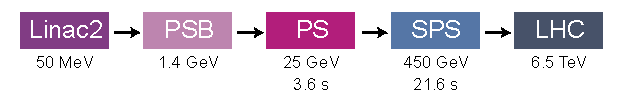
\includegraphics[width=0.8\textwidth]{figures/cms/InjectionChain.pdf}
  \caption[Summary of the injection chain of the LHC.]{Summary of the injection chain of the LHC, including the proton beam energy, which increases at each step, and (for the PS and SPS) the synchrotron cycle time. Multiple cycles of the PS and SPS are required to fill the LHC.}
  \label{cms:injectionchain}
\end{figure}

\Fig~\ref{cms:injectionchain} is a diagram summarizing the injection chain by which protons are accelerated in the LHC.
Protons begin at Linac2, a linear accelerator, and are subsequently injected into the Proton Synchrotron Booster (PSB), the Proton Synchrotron (PS), the Super Proton Synchrotron (SPS), and finally the LHC.
Filling the LHC requires 12 cycles of the SPS and 3--4 cycles of the PS, yielding a total LHC filling time of approximately 4 minutes per beam.

Proton beams at the LHC are not continuous streams of protons, but rather organized into high-intensity bunches spaced 25\unit{ns} apart, corresponding to a crossing frequency of 40\unit{MHz}.
The LHC has 3564 bunch places, of which up to 2808 are filled with protons in colliding bunches.
Consecutive bunches of protons occur in trains of filled bunches separated by gaps.
Proton-proton collisions occur when bunches of protons cross, called bunch crossings.
\Fig~\ref{cms:lhcbunchpattern} is a diagram showing the 3564 bunch places, each represented by a square, and the pattern of filled bunches, represented by squares filled in blue.

\begin{figure}[tpb]
  \centering
  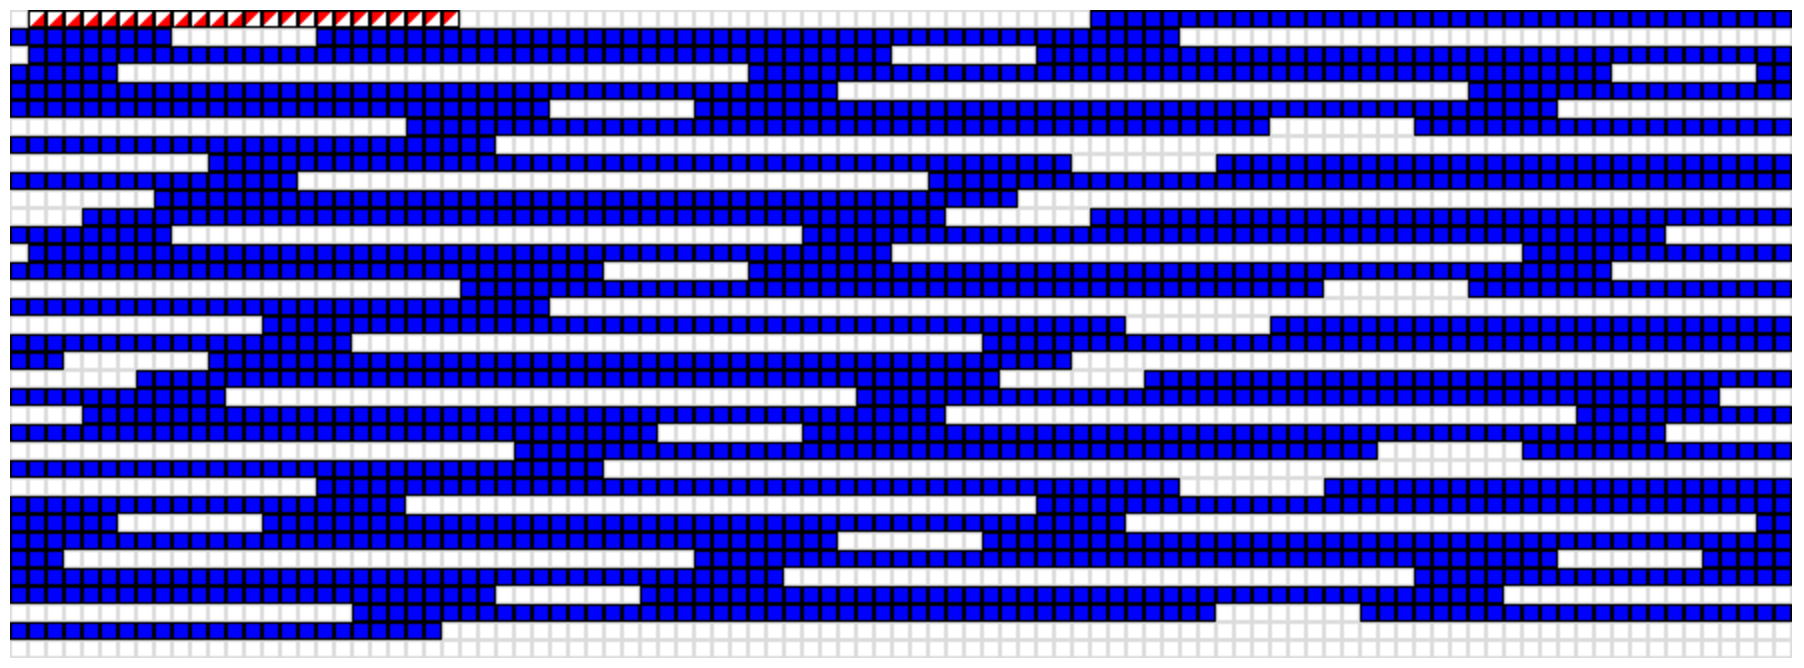
\includegraphics[width=0.8\textwidth]{figures/cms/Fill5423BunchPattern.png}
  \caption[Diagram of the bunch places of an LHC proton beam showing filled and empty places.]{Diagram of the bunch places of an LHC proton beam, showing filled bunches (blue) and empty places (gray). The grid is $99 \times 36 = 3564$ squares, \ie they wrap around. Reproduced from Reference~\cite{CMSWBM:Fill5423} for Fill 5423 of the LHC in October 2016.}
  \label{cms:lhcbunchpattern}
\end{figure}

\subsection{RF Cavities and Steering Magnets}
Protons are accelerated from the 450\GeV of the SPS to the 6.5\TeV of the LHC by a system of eight radio frequency (RF) cavities.
These RF cavities oscillate at 400\unit{MHz} at a maximum amplitude of 2\unit{MV}, for a total of 16\unit{MV} per beam, increasing the proton energy by about 0.5\MeV per revolution.

The phase of the RF waveform is carefully modulated to create and maintain bunches of protons, and to accelerate them to and maintain them at the desired energy.
The 3564 bunch places of the LHC are separated by 25\unit{ns}, meaning a bunch place passes through a particular RF cavity at a frequency of 40\unit{MHz}.
The RF cavity frequency is ten times that: 400\unit{MHz}.
This divides a bunch place into ten RF buckets, which are individual regions of space in which a bunch of protons can be confined, the shape and size of which are determined by the RF voltage amplitude and the number of bunch places.
When coasting (at collision energy), a (hypothetical) particle with energy such that the RF frequency is exactly an integer multiple of the orbit frequency, synchronized such that the particle passes through the RF cavity at exactly a time of zero voltage within the RF waveform is called a synchronous particle.
Particles with higher or lower energy or arriving early or late with respect to the synchronous particle will experience a non-zero voltage and therefore experience a restoring force.
These particles oscillate longitudinally around the synchronous particle.
The size of an RF bucket is given as an area in energy-time phase space, defined with respect to a synchronous particle: it is parametrized by the maximum energy deviation of a particle within the bunch from that of the synchronous particle (in \unit{eV}) and the maximum deviation in arrival time of a particle within the bunch from that of the synchronous particle (in seconds).
A proton bunch occupies a single RF bucket and is depicted by an ellipse within the bucket in energy-time phase space, representing the trajectory of particles within the bunch.
An LHC proton bunch has a 4$\sigma$ bunch length of 1.06\unit{ns} at collision energy.
\Fig~\ref{cms:rfbucket} depicts an RF bucket, football-shaped in energy-time phase space, as well as the ellipse contained within it that represents the proton bunch. The area of the bunch in this diagram is called the longitudinal emittance, with units of $\text{eV}\cdot\text{s}$.

\begin{figure}[p]
  \centering
  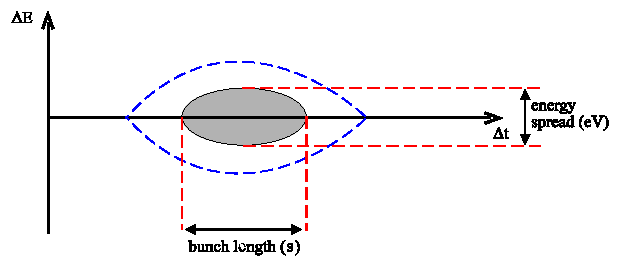
\includegraphics[width=0.8\textwidth]{figures/cms/RFBucket.pdf}
  \caption[Phase space diagram of an RF bucket and the elliptical boundary of a proton bunch within the bucket.]{Phase space diagram of an RF bucket and the elliptical boundary of a proton bunch within the bucket, reproduced from Reference~\cite{Baird:1017689} with minor typographical corrections.}
  \label{cms:rfbucket}
\end{figure}

Beams of particles in the LHC are steered by a network of 1232 superconducting dipole magnets, interspersed with quadrupole magnets for focusing.
The superconducting wire windings in these magnets are made of niobium-titanium, cooled by liquid helium to their operating temperature of 1.9\unit{K}, and producing a magnetic field of 8.33\unit{T}.
\Fig~\ref{cms:dipole} is a diagram of the cross section of an LHC dipole magnet as well as a visualization of the magnetic field lines within the beam pipe.

\begin{figure}[p]
  \centering
  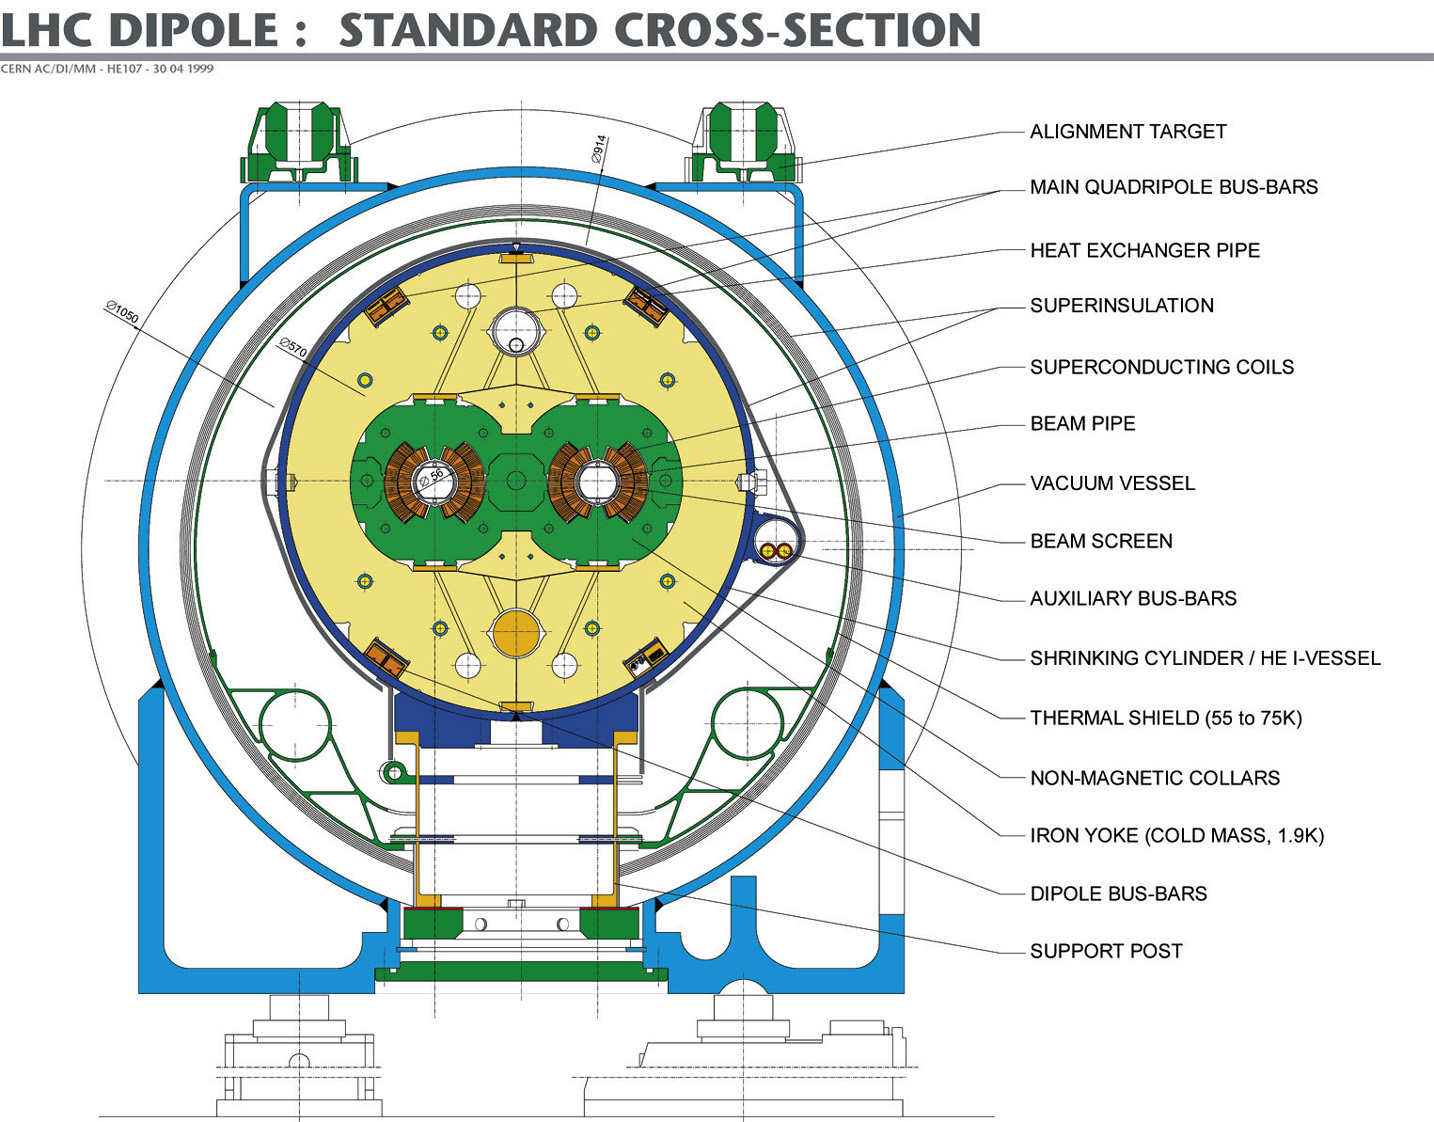
\includegraphics[width=0.55\textwidth]{figures/cms/DipoleCrossSection.jpeg}
  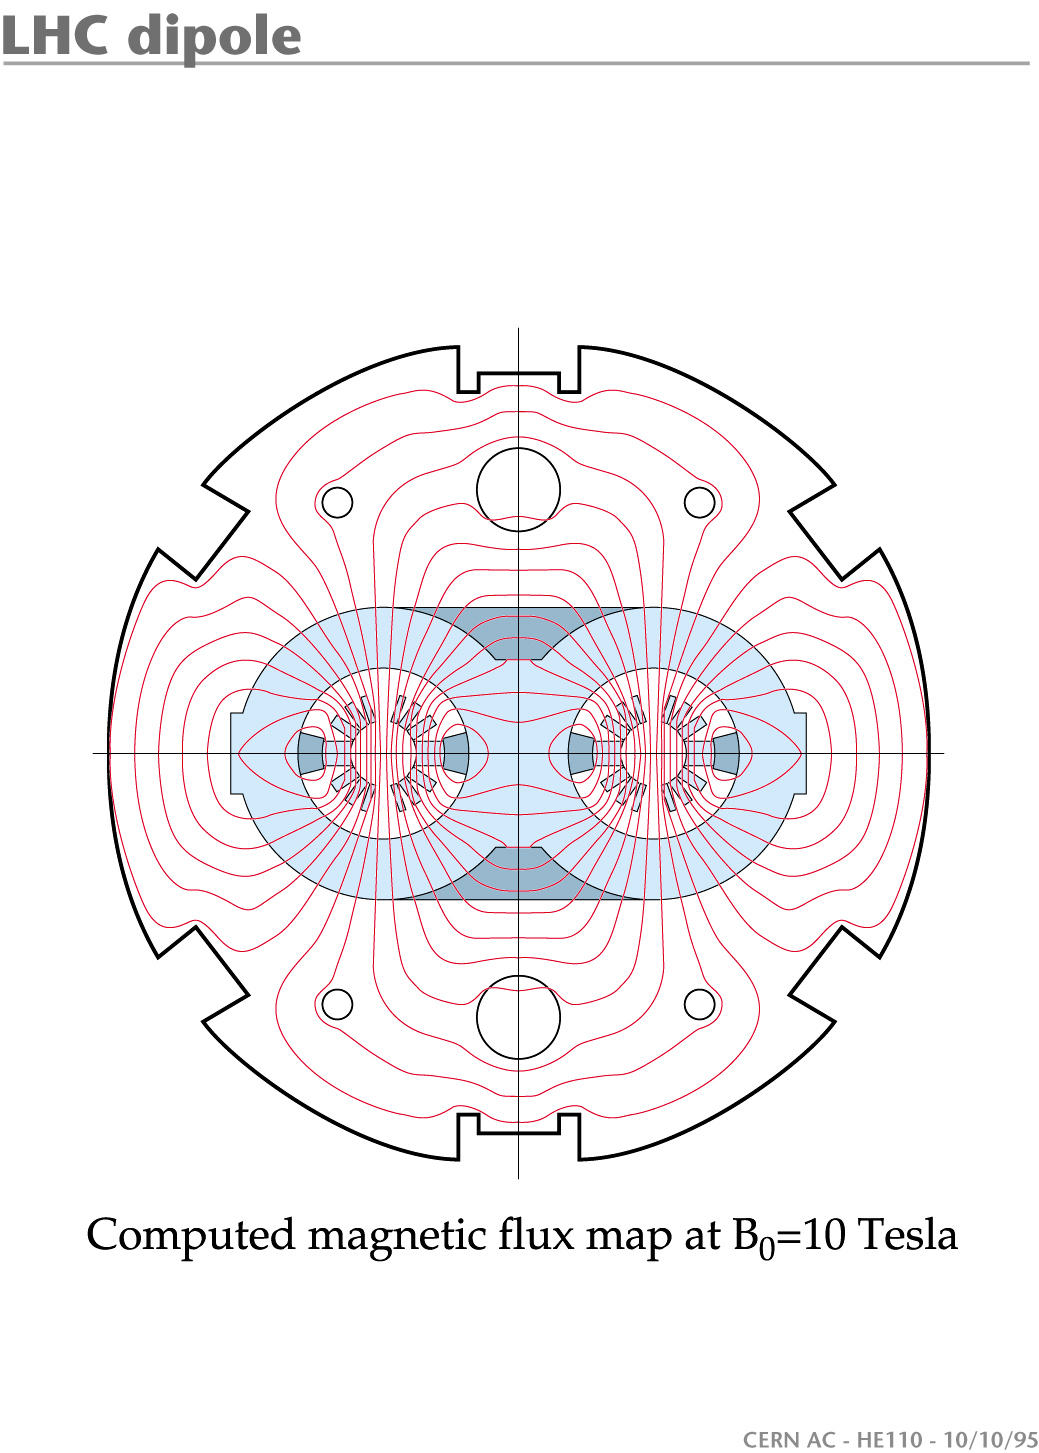
\includegraphics[width=0.35\textwidth]{figures/cms/FieldLines.jpg}
  \caption[Diagram of cross section of an LHC steering dipole magnet and depiction of the magnetic field lines in the magnets.]{(left) Diagram of cross section of an LHC steering dipole magnet, reproduced from Reference~\cite{Team:40524}, showing the two beam pipes and the windings. (right) Depiction of the magnetic field lines in the magnets, reproduced from Reference~\cite{Jean-Luc:841503}, showing them to point in the vertical direction within the beam pipe, as is required to circulate particles along the surface of the earth.}
  \label{cms:dipole}
\end{figure}

\subsection{Instantaneous and Integrated Luminosity}
The number of events per second generated by the LHC for a process of cross section $\sigma$ is
\begin{equation}
  \frac{\dd N}{\dd t} = \lumi \sigma
  \label{cms:nEvents}
\end{equation}
where $\lumi$ is the instantaneous luminosity, and depends only on machine parameters:
\begin{equation}
  \lumi = \frac{N_p^2 N_b f \gamma}{4 \pi \epsilon \beta^*} R 
  \label{cms:instlumi}
\end{equation}
where $R$ is a geometrical factor accounting for the beam crossing angle,
\begin{equation}
  \frac{1}{R} = \sqrt{1 + \left(\frac{\theta\sigma_z}{2\sigma^*}\right)^2}
  \label{cms:geo}
\end{equation}
The design LHC beam parameters in \Eqs~\ref{cms:instlumi}--\ref{cms:geo} are defined and summarized in \Tab~\ref{cms:beam} \cite{Baird:1017689, Bruning:782076}.
This yields a peak instantaneous luminosity of $\lumi = 10^{34} \,  \mathrm{cm}^{-1} \, \mathrm{s}^{-1}$.

\begin{table}
  \centering
  \begin{tabular}{lll}
    \hline
    Symbol     & Name                                                          & Value                 \\ \hline
    $N_p$      & protons per bunch                                             & $1.15 \times 10^{11}$ \\
    $N_b$      & bunches per beam                                              & 2808                  \\
    $f$        & revolution frequency (1/24.95\unit{ns}/3564)                  & 11.25\unit{kHz}       \\
    $\gamma$   & relativistic Lorentz factor for protons ($E_p/m_p$)           & 7461                  \\
    $\epsilon$ & normalized transverse beam emittance                          & 3.75\mum              \\
    $\beta^*$  & optical $\beta$ function (amplitude of betatron oscillations) & 55\unit{cm}           \\
    $\theta$   & beam crossing angle                                           & 285 $\mu\text{rad}$   \\
    $\sigma_z$ & longitudinal RMS bunch length                                 & 7.55\unit{cm}         \\
    $\sigma^*$ & transverse RMS beam size                                      & 16.7\mum              \\
    & & \\ \hline
  \end{tabular}
  \caption[LHC nominal design beam parameters.]{LHC nominal design beam parameters, reproduced from Reference~\cite{Bruning:782076}.}
  \label{cms:beam}
\end{table}

Proton collisions lead to a natural decrease in luminosity over time, with a luminosity lifetime of 15--25 hours.
The integral of the instantaneous luminosity over time is called the integrated luminosity, $\intlumi$.
The total number of events generated by the LHC for a process of cross section $\sigma$ is then given by the integrated luminosity times the cross section, so that
\begin{align}
  N = \sigma \int{\lumi\,\dd t} = \sigma \intlumi
  \label{cms:intlumi}
\end{align}
Since the \pp interaction cross section is a constant, the total integrated luminosity delivered to (and recorded by) an experiment is therefore also a measure of the number of events and hence the amount of data recorded by the experiment.
For convenience with handling large exponents, the integrated luminosity is given in inverse femtobarns: $1\unit{fb} = 10^{-39}\unit{cm}^2$.
\Fig~\ref{cms:totallumi} is a plot of the total \pp integrated luminosity over time, by year and calendar month, for the entirety of Run~1 and Run~2.
This thesis presents two analyses using data taken by the CMS experiment in 2016: a search for displaced dimuons using the full 2016 integrated luminosity of 35.9\fbinv, and a study of neutron-induced background in muon chambers using one era of 2016 data taking, corresponding to 8.73\fbinv.

\begin{figure}[tpb]
  \centering
  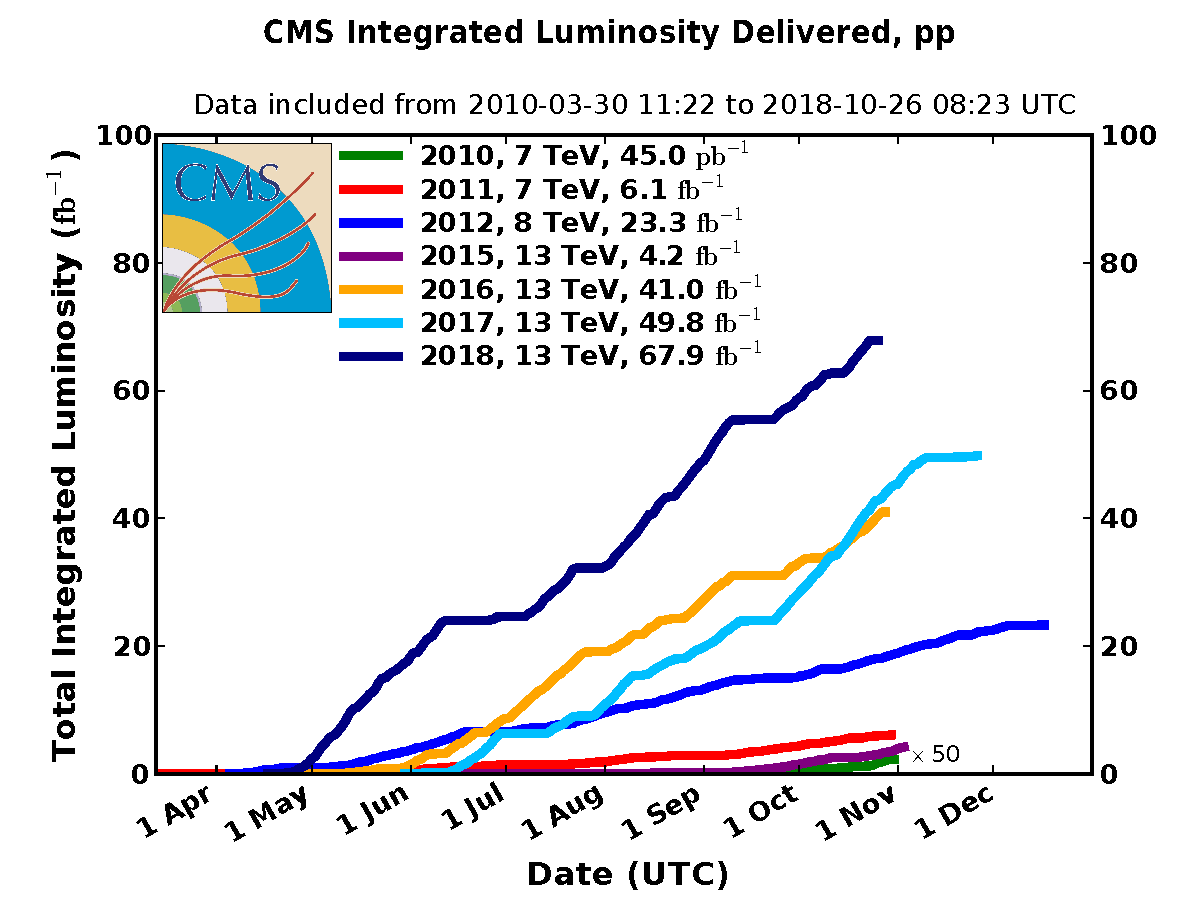
\includegraphics[width=0.8\textwidth]{figures/cms/CMSIntLumi.pdf}
  \caption[Total \pp integrated luminosity recorded by CMS during Run~1 and Run~2 by year and month.]{Total \pp integrated luminosity recorded by CMS during Run~1 and Run~2 by year and month, reproduced from Reference~\cite{LumiTwiki}.}
  \label{cms:totallumi}
\end{figure}

\section{The CMS Detector}
\subsection{Introduction}
\label{cms:intro}
CMS is located at Point~5 of the LHC in the commune of Cessy in eastern France, at the level of the LHC beam line, 100\unit{m} underground.
Its overall shape is a cylinder 15\unit{m} in diameter and 21.6\unit{m} in length, weighing 14,000 tons.
It is named for three of its distinguishing features: its \textbf{c}ompactness, its \textbf{m}uon system, and its \textbf{s}olenoid magnet.
A large magnetic field with high bending power is required to precisely measure the momentum of high-energy charged particles.
This informs a choice of superconducting technology, and so a superconducting solenoid magnet sits at the heart of the cylindrically symmetric CMS detector, producing a continuous magnetic field of 3.8\unit{T}.
CMS is quite compact for all the detector material it contains, especially compared to ATLAS.
Notably, the bulk of the CMS hadronic calorimeter is completely contained the solenoid magnet, with important consequences for its design.
The muon system, on the other hand, is outside the solenoid.
Muons are one of the five general categories of particles directly detected by CMS, and unique among them in that they typically neither stop nor decay within the boundaries of the detector.
They are less subject to energy losses when passing through detector material than electrons and so provide a powerful lens with which to study high-energy processes in the presence of high background.
The outermost bulk of CMS is thus a dedicated system for identifying and measuring muons, consisting of three kinds of gas ionization detectors \cite{Chatrchyan:2008zzk}.

The CMS detector is structured like an onion, in layers, consisting of the following basic subsystems, ordered from innermost to outermost:
\begin{itemize}
  \item silicon tracker
  \item electromagnetic calorimeter
  \item hadronic calorimeter
  \item superconducting solenoid magnet
  \item muon system
\end{itemize}

\Fig~\ref{cms:interactive} is a diagram of a slice of the CMS detector illustrating these layers.
\begin{figure}[tpb]
  \centering
  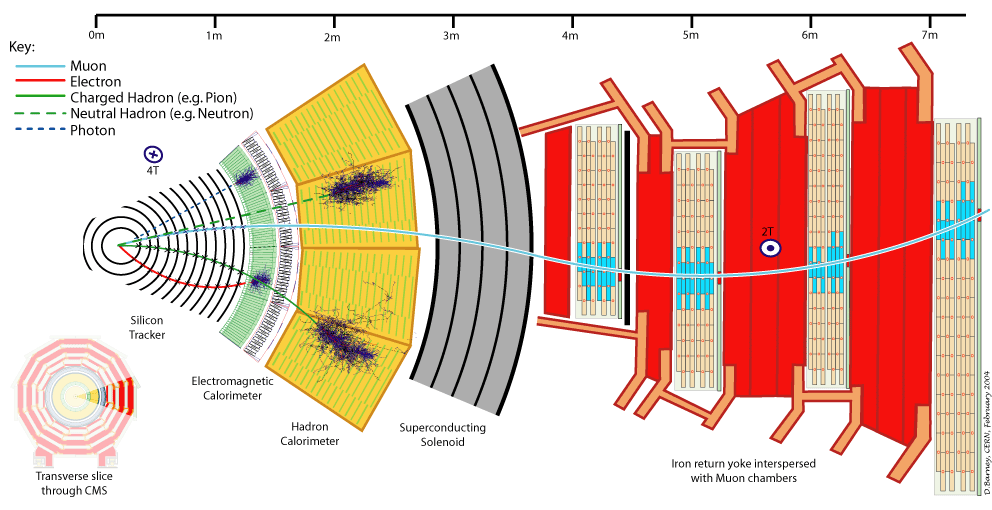
\includegraphics[width=\textwidth]{figures/cms/CMSSlice.png}
  \caption[Transverse slice of the CMS detector illustrating the basic structure of CMS and the shapes of the tracks and energy deposits formed by the five general categories of particles directly detected by CMS.]{Transverse slice of the CMS detector, reproduced from Reference~\cite{Davis:2205172}, illustrating the basic structure of CMS and the shapes of the tracks and energy deposits formed by the five general categories of particles directly detected by CMS by one or more of its subsystems.}
  \label{cms:interactive}
\end{figure}
It also shows the detector signatures of the general categories of particles directly detected by CMS:
\begin{itemize}
  \item electrons
  \item photons
  \item charged hadrons
  \item neutral hadrons
  \item muons
\end{itemize}
The charged particles---electrons, muons, and charged hadrons---are detected as they form curved, helical tracks in the silicon tracker (and in the case of muons, in the muon system as well).
Electrons, charged hadrons, and the neutral particles---photons and neutral hadrons---leave energy deposits in the electromagnetic and hadronic calorimeters.

\subsection{Coordinate System}
The origin of the coordinate system used by CMS is the nominal \pp collision point.
The $y$-axis points upwards, the $x$-axis points radially inwards towards the center of the LHC, approximately south, and thus the $z$-axis points approximately west.
The azimuthal angle $\phi$ about the $z$-axis is measured from the $x$-axis and the radial coordinate in the $xy$-plane is denoted $r$.
The polar angle measured from the $z$-axis is denoted $\theta$.
However, a more conventional coordinate used in hadron collider physics is the pseudorapidity $\eta$, defined as
\begin{equation}
  \eta = -\ln\tan\left(\frac{\theta}{2}\right)
  \label{eq:eta}
\end{equation}
For a particle of three-momentum $\vc{p}$ with $z$-component $p_z$, pseudorapidity can be written
\begin{equation}
  \eta = \frac12\ln\left(\frac{|\vc{p}|+p_z}{|\vc{p}|-p_z}\right)
  \label{eq:eta_p}
\end{equation}
This form elucidates its relationship to rapidity (along the $z$-axis),
\begin{equation}
  y = \frac12\ln\left(\frac{E+p_z}{E-p_z}\right),
  \label{eq:rap}
\end{equation}
which is a quantity Lorentz invariant under boosts in the $z$-direction \cite{Hama:1981}.
The pseudorapidity has the advantage that it converges to rapidity (along the $z$-axis) in the high-velocity, low-mass limit (as $|\vc{p}|\to E$), and is only dependent on the polar angle $\theta$ and not on the energy of the particle.
\Fig~\ref{cms:quadrant} is a schematic diagram of one quadrant of CMS, showing the placement of the components of CMS within the coordinate system.
\begin{figure}[tpb]
  \centering
  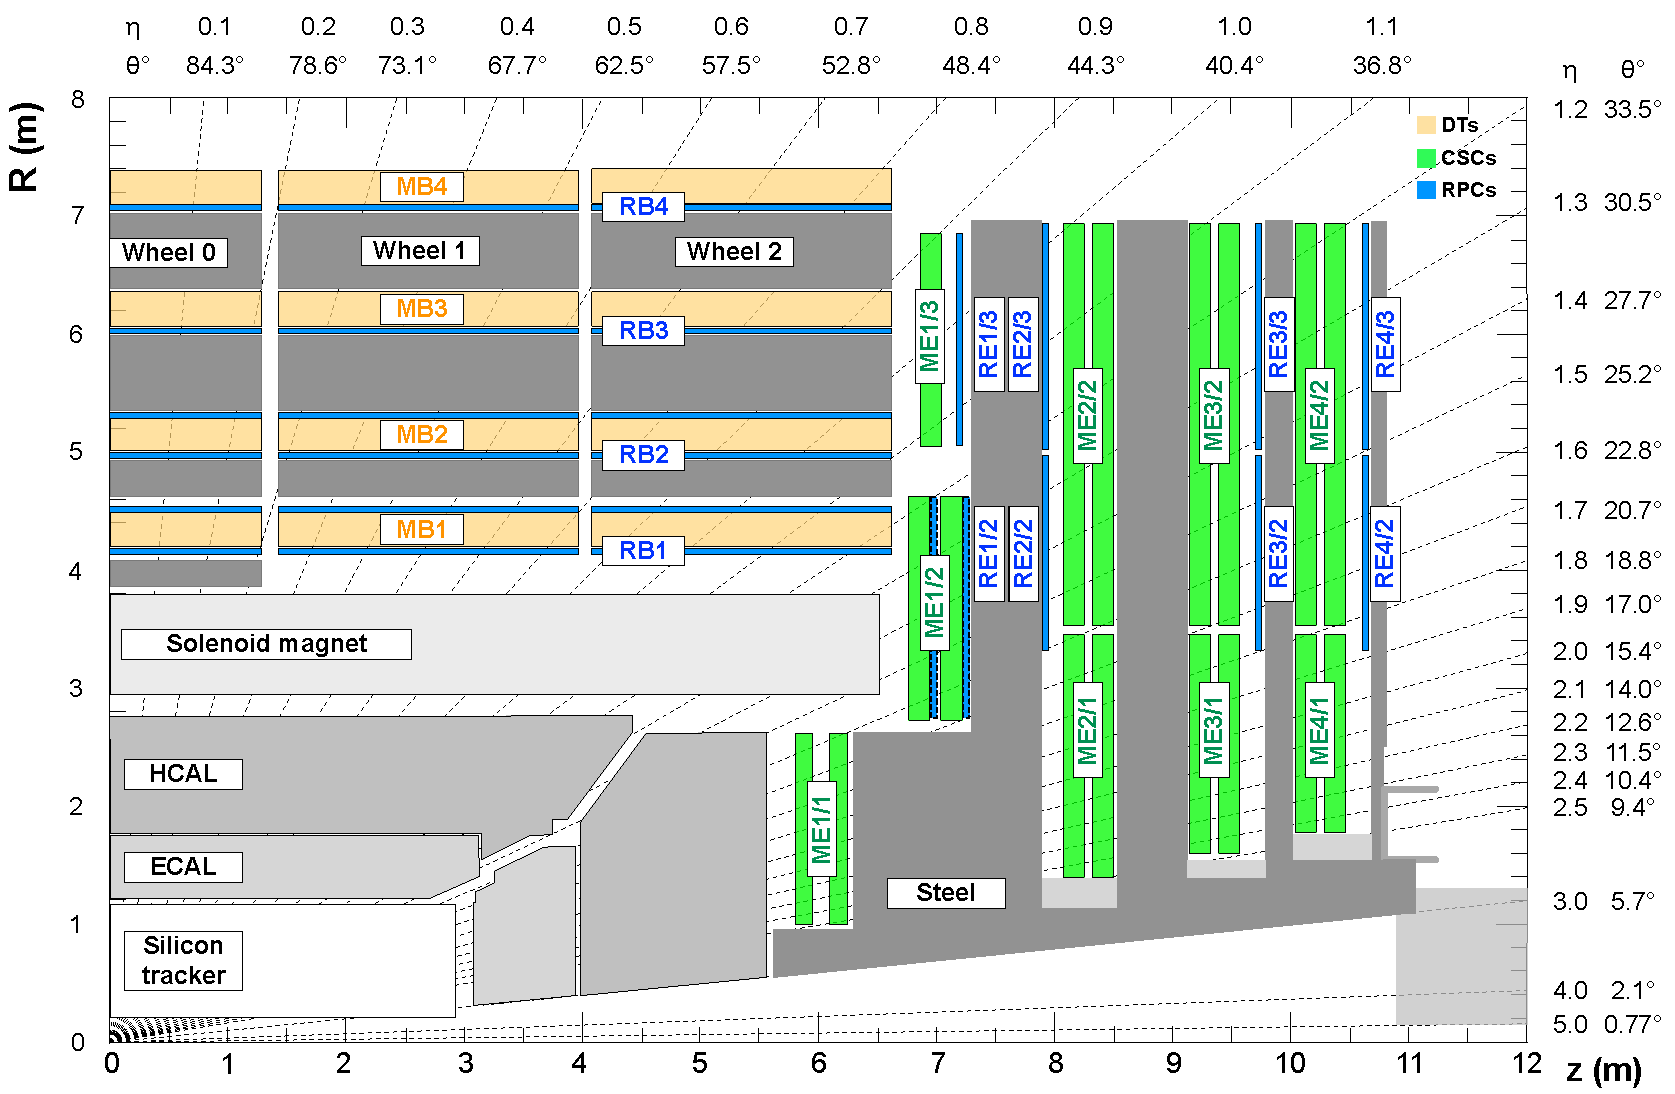
\includegraphics[width=\textwidth]{figures/cms/CMSGeometry.pdf}
  \caption[Schematic diagram of one quadrant of CMS in $r$-$z$.]{Schematic diagram of one quadrant of CMS in $r$-$z$, reproduced from Reference~\cite{Sirunyan:2018fpa}, illustrating the position of all the subsystems with respect to the coordinate system, in both the barrel and the endcap.}
  \label{cms:quadrant}
\end{figure}

The diagram illustrates that $\eta = 0$ points upwards, while $\eta \to \infty$ points along the $z$-axis.
For this reason the ``forward'' regions close to the beam line (which are also less instrumented) are referred to as ``high $\eta$.''
The diagram also illustrates two distinct loci within the CMS detector: the barrel, which covers approximately (depending on subsystem) the region $|\eta| < 1.2$, and the endcap, which covers approximately (depending on subsystem) the region $1.2 < |\eta| < 3$.

\subsection{Silicon Tracker}
The inner tracking system of CMS must provide precise measurements of charged particle trajectories and reconstructions of secondary vertices of (on average) a thousand particles every 25\unit{ns} bunch crossing, exposed to the full flux of the radiation of the LHC.
These requirements on precision, speed, and radiation hardness inform a choice of silicon detector technology.
The ionization induced by an energetic charged particle passing through produces electron-hole pairs, which are measured as current in the presence of an applied voltage.

The CMS tracker consists of two silicon detector technologies: pixels and strips.
The innermost component of the tracker, closest to the collision point, is the pixel detector, consisting of three barrel layers and two endcap disks on each side of the barrel.
The 66 million silicon pixel sensors are $n$-on-$n$ devices, measuring $100 \mum \times 150 \mum$, giving a spatial resolution of 15--20\mum.
Just outside the pixel detector is the strip detector, consisting of ten barrel layers and twelve endcap disks on each side of the barrel.
The 9.6 million silicon strip sensors are $p$-on-$n$ type microstrip sensors, manufactured on 6\unit{in} wafers, varying in width from 80--180\mum.
The CMS tracker measures transverse momentum ($\pT$) to a resolution of 1\% for 100\GeV particles.
Containing altogether 205~$\text{m}^2$ of silicon sensors with 75 million individual channels, the CMS tracker is the largest silicon detector in the world \cite{Chatrchyan:2008zzk, CERN-LHCC-98-006, HARTMANN201225}.


\subsection{Electromagnetic Calorimeter}
The electromagnetic calorimeter (ECAL) was designed to achieve the excellent energy resolution critical for observing the decay of the SM Higgs boson to two photons: $H \to \gamma\gamma$.
The ECAL is a homogeneous calorimeter consisting of about 76,000 scintillating lead tungstate (PbWO$_4$) crystals, a material chosen for its high density and short radiation length.
Electrons or photons passing through the detector material result in a cascade of electromagnetic interactions, producing a shower of particles culminating in a release of energy proportional to the energy of the incident particle.
The corresponding photons are then measured by photodetectors installed on each crystal \cite{Chatrchyan:2008zzk, CERN-LHCC-97-033, Fabjan:692252}.

\subsection{Hadronic Calorimeter}
The hadronic calorimeter (HCAL) is a sampling calorimeter: it consists of repeating, alternating layers of an absorber, which interacts with an incident particle to produce more particles of lower energy, and an active medium, which provides a detectable signal.
This is in contrast to a homogeneous calorimeter, like the ECAL, in which a single type of material performs both functions.

The HCAL consists of four parts: the barrel and endcap HCAL (HB and HE), the outer HCAL (HO), and the forward HCAL (HF).
In the HB and HE, the absorber material consists of thick tiles of brass, and the active medium consists of thinner tiles of scintillating plastic with wavelength-shifting readout fibers.
Brass is a dense material with many nuclei to interact strongly with incident hadron showers.
It is also non-magnetic, a necessary property of the absorber for the HB and HE, which lie within the solenoid and experience its full 3.8\unit{T} magnetic field.

As the HB and HE lie within the solenoid and hence are only about 6 interaction lengths thick, the first layer of the muon system is instrumented with scintillator tiles, treating the solenoid as an additional absorber.
This ``tail catcher'' is known as the outer calorimeter, or HO.

The HF is located 11\unit{m} from the interaction point, in the pseudorapidity range of approximately $3.0 < |\eta| < 5.0$.
This forward region experiences very high levels of LHC radiation and thus is constructed out of radiation-hard materials: steel for the absorber and quartz fiber for the active material, which detects the Cherenkov radiation produced by energetic jets \cite{Chatrchyan:2008zzk, CERN-LHCC-97-031, Penzo2009}.

\subsection{Solenoid Magnet}
The CMS magnet is a superconducting solenoid, 12.5\unit{m} long with an inner diameter of 6.3\unit{m}. Liquid helium cools the magnet to its superconducting operating temperature of 4\unit{K}. It draws 19\unit{kA} of current and is the largest magnet in the world in terms of its 2.6\unit{GJ} of stored energy.

A powerful magnetic field is crucial for precise momentum measurement of high-energy charged particles.
As an introduction to issues related to muon \pT measurement, consider a charged particle of charge $q$ and transverse momentum $\pT = \vc{p} \cdot \hat{\vc{r}}$ in a uniform magnetic field of strength $B$ pointing in the $z$-direction, which is a good model for a charged particle in the CMS tracker. Such a particle travels in a helix of (signed) radius
\begin{equation}
  R = \frac{\pT}{qB}
  \label{cms:radius}
\end{equation}
The radius of curvature of a charged particle in a magnetic field is thus proportional to its transverse momentum.
However, what is measured directly is not the radius of curvature, but rather the positions of the hits, whose resolution functions are Gaussian.
To illustrate an important consequence of this, consider \Fig~\ref{cms:sagitta}, which depicts the circular arc left by a charged particle in the tracker.
Let $L$ be the length of the chord joining the outermost points, which is also the radius of the tracker.
Let $s$ be the sagitta, \ie the distance between the midpoint of the chord and the center of the arc.
\begin{figure}[tpb]
  \centering
  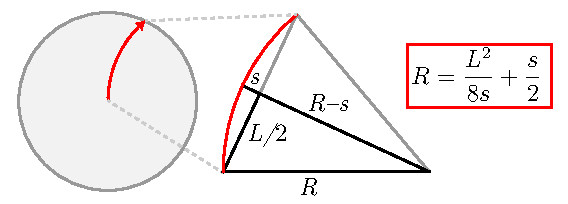
\includegraphics[width=0.8\textwidth]{figures/cms/Sagitta.pdf}
  \caption[Radius of curvature from sagitta.]{Radius of curvature from sagitta. On the left is a depiction of a charged particle leaving a circular arc (red) in the CMS tracker (gray). The length of the chord is $L$, which is also typically the radius of the tracker. The sagitta $s$ is approximately inversely proportional to the radius of curvature $R$, with important consequences for the uncertainty in the desired \pT measurement.}
  \label{cms:sagitta}
\end{figure}
Then $R$, the radius of curvature, can be computed from $L$ and $s$ as follows:
\begin{equation}
  R = \frac{L^2}{8s} + \frac{s}{2} \approx \frac{L^2}{8s}
  \label{cms:eqn_sagitta}
\end{equation}
Since $s$ is typically small compared to $L$, the $s/2$ term can be dropped.
Then $q/\pT$ is approximately proportional to $s$:
\begin{align}
  \frac{q}{\pT} = \frac{1}{BR} \approx \frac{8s}{BL^2}
  \label{cms:pTError}
\end{align}
Since $s$ is linear in the position measurements, its distribution is also Gaussian, and therefore it is the distribution of $q/\pT$, and not $\pT$, that is Gaussian.
The uncertainty on a measurement of \pT obtained from applying standard error propagation to $q/\pT$ must therefore be considered carefully, as it does not describe standard deviations of a variable distributed as a Gaussian.

\subsection{Muon System}
As mentioned in \Sec~\ref{cms:intro}, muon detection is a powerful tool for studying high-energy processes in the presence of high background.
Because of the amount of material in the inner subsystems, typically mostly muons travel through the solenoid.
A track in the muon system therefore is associated with a muon.
Hadronic ``punchthrough'' in the muon system is minimal.

The muon system has three tasks: triggering (\Sec~\ref{cms:trigger}), muon identification, and muon reconstruction.
As with the other subsystems, the shape of the solenoid informs a design of a cylindrical barrel section and an endcap disk section.
Both sections consist of four stations of muon detectors, concentric for the barrel and sequential for the endcap.
The muon system consists of three kinds of gaseous ionization detectors: drift tubes (DT), cathode strip chambers (CSC), and resistive plate chambers (RPC).

The chambers of the muon system are embedded within a set of steel disks in the endcap and concentric twelve-sided steel cylinders in the barrel, referred to as the return yoke.
The return magnetic flux of the solenoid is mostly contained within this return yoke \cite{Chatrchyan:2008zzk, CMS:1997dma}.

\subsubsection{Drift Tubes}
The barrel region of the muon system consists of four stations instrumented with 250 drift tube chambers.
Drift tubes were chosen to be the tracking detectors in the barrel region in light of the low expected rate and relatively low intensity of the local magnetic field.
\Fig~\ref{cms:dt} is a diagram showing the principle of operation of a drift tube cell.
A cathode tube with cross-sectional dimensions $42 \mm \times 13 \mm$ contains an anode wire (operating at 3600\unit{V}) under tension.
The tube is filled with a gas mixture of 85\% Ar and 15\% CO$_2$.
An energetic muon passing through this cell ionizes the gas, and the resulting electrons drift towards the wire.
Measuring the drift time (a maximum of 380\unit{ns}) yields a measurement of position within the cell.

The smallest independent unit of a DT is a superlayer (SL), consisting of four layers of drift cells staggered by a half cell.
A drift tube chamber consists of three (or two) SLs.
The wires in the two outer SLs are parallel to the beam line, and provide a track measurement in the $r$-$\phi$ (bending) plane.
The wires in the inner SL are orthogonal to the beam line, and measure the $z$-position along the beam.
This inner SL is not present in the fourth muon station, which consequently only measures the $\phi$ coordinate.

\begin{figure}[tpb]
  \centering
  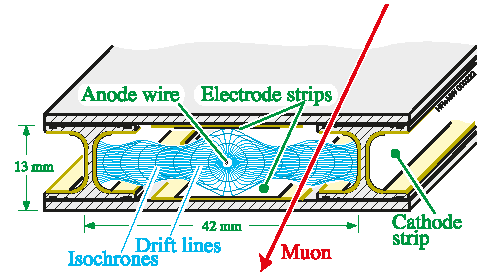
\includegraphics[width=0.8\textwidth]{figures/cms/DT.pdf}
  \caption[Principle of operation of a drift tube cell.]{Principle of operation of a drift tube cell, reproduced from Reference~\cite{Chatrchyan:2013sba}, showing the structure of a cell, as well as the drift lines and isochrones.}
  \label{cms:dt}
\end{figure}

\subsubsection{Cathode Strip Chambers}
The endcap region of the muon system consists of four stations instrumented with 540 cathode strip chambers.
Cathode strip chambers were chosen to be the tracking detectors in the endcap region for their excellent position resolution in the $\phi$ direction achieved by precision cathode charge readout and interpolation.
The CSCs are arranged in circular disks.
Each CSC consists of six layers, each layer lying in an $r$-$\phi$ plane of CMS, consisting of a gas mixture of 50\% CO$_2$, 40\% Ar, and 10\% CF$_4$ in between a plane of copper cathode strips and a plane of anode wires, operating at 2900--3600\unit{V}.
An energetic muon passing through a CSC ionizes the gas, and the resulting electrons drift towards the wires, causing an avalanche of charge that induces an opposite charge on the cathode strips.
Interpolating these charges yields a precise localization of the avalanche.
A more detailed overview of CSCs in the context of a study of neutron-induced background is given in \Sec~\ref{sec:csc_electronics}.

\subsubsection{Resistive Plate Chambers}
Interspersed throughout both the barrel and endcap muon system are 480 and 576 resistive plate chambers, respectively, whose purpose is a fast time response and resolution comparable to that of scintillators.
RPCs therefore are part of a dedicated muon trigger for identifying muon tracks and assigning the bunch crossing with high efficiency.
An RPC consists of two parallel plates of phenolic resin coated with conductive graphite, with a 2\mm gap filled with a gas mixture of 95.2\% freon (C$_2$H$_2$F$_4$, known as R134a), 3.5\% isobutane (i-C$_4$H$_{10}$), and 0.3\% sulfur hexafluoride (SF$_6$).
An energetic muon crossing the chamber ionizes the gas and induces an image charge, which is sampled and read out.
The RPCs have a time resolution of about 2\unit{ns}, a much shorter time than the 25\unit{ns} between LHC bunch crossings, but much coarser position resolution than DTs or CSCs.

\subsubsection{Muon Momentum Resolution}
An important consequence of a dedicated muon system for reconstructing muons is that it improves the \pT resolution for muons at high muon \pT.
\Fig~\ref{cms:muonpT} shows plots of the muon \pT resolution using the inner tracking system only, using the muon system only, and combining both, as a function of \pT.
At lower \pT values, the tracker is sufficient to precisely measure the curvature of the muon track, and the tracker-only resolution dominates.
But at higher \pT values, the tracker track is much straighter, and the additional information about muon position obtained from the muon system results in a \pT resolution superior to that obtained by using either system alone.

\begin{figure}[tpb]
  \centering
  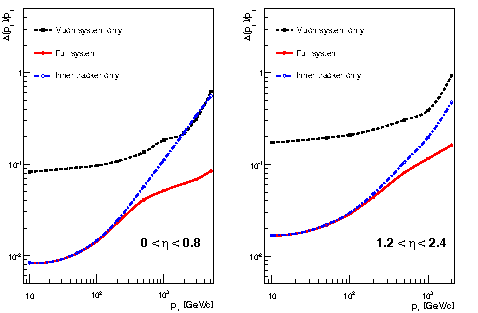
\includegraphics[width=\textwidth]{figures/cms/MuonMomentumResolution.pdf}
  \caption[Muon \pT resolution as a function of muon \pT for the barrel and endcap using the tracking system only, muon system only, and combining both.]{Muon \pT resolution as a function of muon \pT, for (left) the barrel and (right) the endcap, using the inner tracking system only, using the muon system only, and combining both. Reproduced from Reference~\cite{Chatrchyan:2008zzk}.}
  \label{cms:muonpT}
\end{figure}

\subsection{Trigger System}
\label{cms:trigger}
The LHC provides \pp collisions every 25\unit{ns}, corresponding to a crossing frequency of 40\unit{MHz}.
It is impossible to process and store this large amount of data synchronously with such a high rate, and so a rate reduction must be achieved, selecting a subset of the most interesting candidate events for physics analysis.
This rate reduction is performed by the CMS trigger system, an elaborate system of hardware and software that analyzes every bunch crossing and ``triggers'' on potentially interesting events.
The CMS trigger system operates in two steps.
The Level-1 (L1) trigger makes its decisions at the hardware level with custom-built programmable electronics, synchronously with the LHC, and is designed to reduce the rate from 40\unit{MHz} to 100\unit{kHz}.
The High-Level Trigger (HLT) makes its decisions at the software level, performing its computations in real time with respect to the full rate of the LHC, using a processor farm located on the surface at Point~5.
HLT processing operates more slowly than the L1 trigger, but faster than the full event readout, serving to reduce the rate from 100\unit{kHz} to the data acquisition rate of hundreds of Hz \cite{Chatrchyan:2008zzk, Adam:2005zf}.

The L1 trigger consists of a muon trigger and a calorimeter trigger, organized into local, regional, and global components.
Both the ECAL and all components of the HCAL participate in the calorimeter trigger, and all three muon chambers---DTs, CSCs, and RPCs---participate in the muon trigger, the first muon trigger to measure momentum at the hardware Level-1.
The local components are the lowest level, based on energy deposits in the calorimeters and hits and segments in the muon system.
Regional components combine the information from the local components using pattern recognition and track finding and rank trigger objects in small regions.
The global components determine the highest-rank objects and transfer them to the global trigger of the L1 system.
The global trigger then makes the decision to reject or accept the event at Level-1.
A Level-1 Accept (L1A) decision is communicated to the subsystems and the event is passed to the HLT for further evaluation.
The L1 trigger must analyze every bunch crossing, doing so with a maximum latency of 3.2\mus.
\Fig~\ref{cms:L1} depicts the architecture of the L1 trigger.

\begin{figure}[tb]
  \centering
  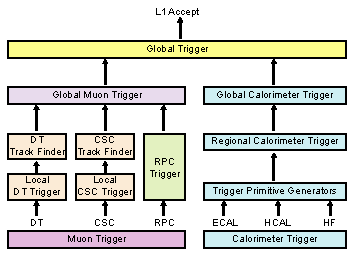
\includegraphics[width=0.8\textwidth]{figures/cms/L1Architecture.pdf}
  \caption[Architecture of the L1 trigger system, depicting the local, regional, and global components of the muon and calorimeter triggers.]{Architecture of the L1 trigger system, based on a figure from Reference~\cite{Chatrchyan:2008zzk}, depicting the local, regional, and global components of the muon and calorimeter triggers, the information from which is processed by the global L1 trigger for trigger decision at L1.}
  \label{cms:L1}
\end{figure}

\pagebreak
The L1 and HLT menus consists of paths that define criteria on which to trigger.
These criteria are the first step to any physics analysis, and so can include requirements on \pT, on numbers of muons or jets, on the geometry and angles between them, and much more.
The HLT uses information from the entire detector, with high-level algorithms that make a more precise decision than the coarser L1 trigger.
Each HLT path is seeded by one or more L1 paths and is designed to be inclusive and general while keeping the event rate in the data acquisition system within its maximum rate.


\chapter{Search for Long-Lived Particles Decaying to Displaced Dimuons in the CMS Muon System at \texorpdfstring{$\bm{\sqrt{s}}$}{\textbf{sqrt(s)}} = \texorpdfstring{13\TeV}{13~TeV}}
\label{chap:displaced}
\PretentiousQuoteWithAuthor{When you have eliminated the impossible, whatever remains, however improbable, must be the truth.}{Sherlock Holmes}{The Sign of the Four}{Sir Arthur Conan Doyle}

This chapter presents a search for long-lived particles decaying to two muons in the CMS detector with data taken in 2016 at center-of-mass energy $\sqrt{s} = 13\TeV$ corresponding to 36.3\fbinv of integrated luminosity during Run~2 of the LHC.
The reconstructed muons form dimuon vertices displaced with respect to the \pp collision interaction point, giving rise to a variety of interesting experimental challenges.
This analysis focuses on muons reconstructed using only the muon system of CMS, and is a continuation and extension of two CMS analyses \cite{EXO-12-037,CMS-PAS-EXO-14-012} performed with data taken at center-of-mass energy $\sqrt{s} = 8\TeV$ during Run~1 of the LHC.
The results are interpreted in the context of the BSM Higgs model introduced in Chapter~\ref{chap:theory}, but the search is meant to be inclusive and model-independent.

\section{Trigger, Data, and Simulation}
\subsection{Trigger}
\label{sec:dd:Trigger}
The choices of trigger paths determine which events in data are used in the analysis.
Typical CMS analyses using muons search for new particles produced in the hard interactions of \pp collisions that decay quickly into muons.
Such muons appear to originate directly from the point of interaction of the crossing beams, or beam spot.
For this reason, the reconstruction of muon tracks used by most trigger paths includes knowledge of the beam spot, referred to as a beam spot constraint.
But muons produced from the decay of a long-lived particle may not point towards the beam spot.
Therefore, dedicated triggers without beam spot constraints are necessary to collect data containing long-lived particles.

The HLT path that collected the 2016 data studied in this analysis was
$$\Code{HLT\_L2DoubleMu28\_NoVertex\_2Cha\_Angle2p5\_Mass10}$$
The abbreviations in this expression define the various criteria:
\begin{itemize}
  \item \texttt{\textbf{L2DoubleMu28}}: requirement that two muons be reconstructed using only the muon system, each with a $\pT$ of at least 28\GeV. The muon system requirement is the first step towards ensuring that the triggered objects are really muons, as well as allowing the analysis to be sensitive to a range of possible lifetimes. The \pT requirement keeps the rate of triggered events in the data acquisition system within its maximum rate and allows the analysis to focus on events in a regime with reduced contributions from complex QCD processes.
  \item \texttt{\textbf{NoVertex}}: requirement that no beam spot constraint be imposed in the muon reconstruction.
  \item \texttt{\textbf{2Cha}}: requirement that muon segments be present in at least two CSC or DT stations. This requirement selects muons with hits over multiple chambers, which is necessary to reconstruct them with high quality.
  \item \texttt{\textbf{Angle2p5}}: requirement that the 3D angle between the muons $\alpha$ be at least 2.5\unit{rad} (equivalent to $\cos{\alpha} > -0.8$). This requirement is intended to prevent cosmic muons from passing the trigger, as the reconstruction algorithms usually reconstruct cosmic muons as a pair of back-to-back muons, \ie $\alpha \approx \pi$ or $\cos{\alpha} \approx -1$.
  \item \texttt{\textbf{Mass10}}: requirement that the invariant mass of the two muon system \mMuMu be at least 10\GeV. As with the \pT requirement above, this requirement also serves to keep the event rate within acceptable thresholds and to reduce consideration of events dominated by complex QCD processes.
\end{itemize}

\subsection{Data Samples}
The analysis uses data taken from \pp collisions at the LHC center-of-mass energy of 13\TeV during the data taking period of 2016, corresponding to an integrated luminosity of 36.3\fbinv.
The CMS datasets used are reprocessed under the CMS software version \Code{CMSSW\_8\_0\_31} in August 2017, known as the ``re-reco'' data.
CMS data are organized into runs consisting of many individual lumi sections, which are time intervals of data taking at CMS corresponding to approximately 23\unit{s}.
A dedicated data quality management team certifies CMS data by producing lists of run numbers approved for physics analysis.
\Tab~\ref{tab:dd:datasamples} lists the names of the datasets used in this analysis, their certified run range, and their corresponding integrated luminosity for each of the data taking eras of 2016.

\begin{table}
  \centering
  \begin{tabular}{lcr}
    \hline
    Dataset & Run Range & \multicolumn{1}{c}{\intlumi} \\
    \hline
    \Code{DoubleMuon/Run2016B-07Aug17\_ver2-v1/AOD} & 273150--275376 &          5.81\fbinv  \\
    \Code{DoubleMuon/Run2016C-07Aug17-v1/AOD}       & 275656--276283 &          2.62\fbinv  \\
    \Code{DoubleMuon/Run2016D-07Aug17-v1/AOD}       & 276315--276811 &          4.28\fbinv  \\
    \Code{DoubleMuon/Run2016E-07Aug17-v1/AOD}       & 276831--277420 &          4.03\fbinv  \\
    \Code{DoubleMuon/Run2016F-07Aug17-v1/AOD}       & 277932--278808 &          3.12\fbinv  \\
    \Code{DoubleMuon/Run2016G-07Aug17-v1/AOD}       & 278820--280385 &          7.66\fbinv  \\
    \Code{DoubleMuon/Run2016H-07Aug17-v1/AOD}       & 281613--284044 &          8.77\fbinv  \\
    \hline
    \textbf{Total}                                  &                & \textbf{36.30\fbinv} \\
    \hline
  \end{tabular}
  \caption[CMS datasets used by the analysis, including dataset names, the ``Muon Physics'' run ranges as certified by CMS for physics analysis, and integrated luminosities.]{CMS datasets used by the analysis, including dataset names, the ``Muon Physics'' run ranges as certified by CMS for physics analysis, and integrated luminosities, taken from Reference~\cite{PdmV2016} and following embedded links. Integrated luminosity values were obtained from running the standard \Code{brilcalc} prescription found at Reference~\cite{BrilcalcQuickStart}.}
  \label{tab:dd:datasamples}
\end{table}

\subsection{Monte Carlo Simulation Samples of Signal and Background}
\label{sec:dd:mcsamples}
Comparing theoretical predictions to CMS data is a complex task that must connect scattering amplitudes of the hard process underlying the \pp collision computed via perturbative methods in quantum field theory, to the production of particles and their passage through the material of CMS, to the response and subsequent data obtained by the CMS detectors.
Numerical simulation is used to obtain these predictions.
Because Monte Carlo methods are used to model stochastic effects at each stage, this simulation is described as Monte Carlo (MC) simulation.
This analysis uses simulation of signal models as well as simulation of background processes in its studies.

\Tab~\ref{tab:dd:signalsamples} lists the MC simulation samples of the BSM Higgs $\PHiggs \to \PLLP\PLLP$ benchmark signal model described in Chapter~\ref{chap:theory}.
Both \fourMu final states, in which both long-lived particles decay to two muons, and \twoMu final states, in which one long-lived particle decays to two muons and the other does not, are simulated.
Samples were produced for several combinations of BSM Higgs masses (\mH), long-lived particle masses (\mX), and long-lived particle lifetimes (\cTau).
In order to study decays occurring everywhere from near the beam spot to the beginning of the muon system, the long-lived particle lifetimes were chosen such that the mean decay lengths in the transverse plane are 3\cm, 30\cm, and 250\cm in the laboratory frame.
These signal samples can be reweighted to study additional intermediate lifetimes.

\begin{table}
  \centering
  \begin{tabular}{ccccc}
    \hline
    \mH (\GeVns) & \mX (\GeVns) & \multicolumn{3}{c}{\cTau (\mm)} \\
    \hline
    \multirow{4}{*}{1000} & 350 & 35 & 350 & 3500 \\
                          & 150 & 10 & 100 & 1000 \\
                          &  50 &  4 &  40 &  400 \\
                          &  20 &  2 &  20 &  200 \\
    \hline
    \multirow{3}{*}{400}  & 150 & 40 & 400 & 4000 \\
                          &  50 &  8 &  80 &  800 \\
                          &  20 &  4 &  40 &  400 \\
    \hline
    \multirow{2}{*}{200}  &  50 & 20 & 200 & 2000 \\
                          &  20 &  7 &  70 & 7000 \\
    \hline
    \multirow{2}{*}{125}  &  50 & 50 & 500 & 5000 \\
                          &  20 & 13 & 130 & 1300 \\
    \hline
  \end{tabular}
  \caption{Simulated $\PHiggs \to \PLLP\PLLP$ signal samples used by the analysis, for several combinations of BSM Higgs mass (\mH), long-lived particle mass (\mX), and long-lived particle lifetime (\cTau).}
  \label{tab:dd:signalsamples}
\end{table}

The main backgrounds for this analysis are
\begin{itemize}
  \item the Drell-Yan process yielding dileptons ($\pp\to\PZ/\gamma^* \to \ell\ell$), especially from reconstruction mistakes;
  \item QCD processes yielding dileptons, especially from decays of bottom and charm quarks and hadron decays in flight; and
  \item cosmic muons reconstructed as dileptons
\end{itemize}
Other backgrounds from top quark production and diboson production with leptonic decays produce negligible contributions.
The CMS collaboration centrally produces MC simulation of background processes for physics analysis; this analysis uses the ``Summer16'' campaign produced for the winter conferences of 2017.
\Tab~\ref{tab:dd:bgsamples} lists the MC simulation samples of background processes used in this analysis, with the total production cross section and the number of generated events, and an ``equivalent luminosity'' (defined in \Sec~\ref{sec:dd:EqLumi}) that is important for understanding the statistical power of the simulation.
These MC background samples are useful for many studies, but have some important limitations:
\begin{itemize}
  \item The Drell-Yan and QCD processes are the dominant sources of background events in \pp collisions and are simulated. However, the reconstruction mistakes producing this background may not be well modeled, and the simulation of QCD events is known to not accurately reproduce data in the tails of some distributions.
  \item The Drell-Yan and QCD samples also have limited statistical power, as the number of generated events is fewer than the number of expected events in 2016 data.
  \item The available MC simulation of cosmic muons does not include simulation of multiple cosmic muons from a single atmospheric shower (showers of cosmic muons) or of cosmic muons mixed with \pp collisions.
\end{itemize}
For these reasons, MC simulation of background does not provide a good description of the expected background, so optimization of the analysis as well as evaluation of the expected background is consequently performed using data.
MC simulation of background is therefore primarily used to study general trends and to gain insights.

\begin{table}
  \centering
  \begin{tabular}{llD{.}{.}{6.3}rD{.}{.}{3.2}}
    \hline
    Process & Kinematic Cuts & \multicolumn{1}{c}{$\sigma$ (\unit{pb})} & Events & \multicolumn{1}{c}{$\intlumi^\text{eq}$ (\fbinv)} \\
    \hline
    \PZ/$\gamma^* \to \ell\ell$        & $10\GeV < m_{\ell\ell} < 50\GeV$ &  18810     &   30,935,823 &   1.20\\
    \PZ/$\gamma^* \to \ell\ell$        & $m_{\ell\ell} > 50\GeV$          &   6225     &  122,547,040 &  13.19\\
    QCD \Pgm-enriched                  & $\pT > 20\GeV$                   & 302672.16  &   22,094,081 &   0.07\\
    $\ttbar \to \ell\ell\nu\nu$        &                                  &     87.31  &   79,140,880 & 906.44\\
    \Ptop\PW, \Ptbar\PW                &                                  &     35.8   &   13,885,924 & 387.87\\
    \PW\PZ                             &                                  &     47.13  &    6,995,142 &  84.82\\
    \PZ\PZ                             &                                  &     16.523 &    2,986,132 & 120.32\\
    $\PW\PW\to \ell\ell\nu\nu$         &                                  &     12.178 &    1,999,000 & 164.15\\
    \PW+jets                           &                                  &  61526.7   &   29,804,825 &   0.48\\
    \hline
  \end{tabular}
  \caption[CMS simulation samples used by the analysis for each background process, along with the total production cross section and the number of generated events.]{CMS simulation samples used by the analysis for each background process, along with the total production cross section and the number of generated events. The equivalent luminosity in 2016 $\intlumi^\text{eq}$ is the proportionality factor that is used to scale simulated events to correspond to the total integrated luminosity in 2016 (36.3\fbinv).}
  \label{tab:dd:bgsamples}
\end{table}

Simulation of the hard process including matrix element computation is performed by \POWHEG2 \cite{Nason:2004rx,Frixione:2007vw,Alioli:2010xd} in all signal and background samples, except for the Drell-Yan ($\PZ/\gamma^* \to \ell\ell$) sample, whose hard process is simulated by \MGvATNLO 2.2.2 \cite{Alwall:2014hca}, and the \PW+jets sample, whose hard process is simulated by \MADGRAPH5 \cite{Alwall:2011uj}.
Simulation of parton showering and hadronization is performed by \PYTHIA8.212 using the CUETP8M1 tune \cite{Sjostrand:2014zea,Khachatryan:2015pea} in all signal and background samples except for the \PW\PW\ sample, whose parton showering is simulated by \HERWIGpp2.7.1 \cite{Bahr:2008pv}.
Simulation of the passage of particles through detector material and the induced response in detector electronics is performed by \GEANTfour \cite{Agostinelli:2002hh,Allison:2006ve,Allison:2016lfl}.

\subsection{Equivalent Luminosity and Event Weighting in MC Simulation}
\label{sec:dd:EqLumi}
Because the number of simulated events is not equal to the number of expected events in data, comparing simulation to data requires that the contribution of each event be scaled by a weight factor depending on the cross section and the number of events.
This weight factor can be understood in terms of an ``equivalent integrated luminosity.''
Given a number of generated events $N_\text{events}$ and a cross section of $\sigma$, the equivalent luminosity is
\begin{equation}
  \intlumi^\text{eq} = \frac{N_\text{events}}{\sigma}
  \label{eq:dd:eqlumi}
\end{equation}
Then, when comparing to \intlumi of data, the contribution of each simulated event is scaled by the weight factor
\begin{equation}
  w = \frac{\intlumi}{\intlumi^\text{eq}} = \frac{\sigma\intlumi}{N_\text{events}}
  \label{eq:dd:mcweightpre}
\end{equation}
In practice, two additional subtleties modify \Eqs~\ref{eq:dd:eqlumi}--\ref{eq:dd:mcweightpre}.
First, corrections the cross section $\sigma$ when passing from leading-order to next-to-leading-order are given as a scaling factor $k$.
This is accounted for by the substitution $\sigma \to \sigma \, k$.
Second, matrix element computations performed by \MGvATNLO assign a negative contribution to some events, according to the sign of the contributing diagrams.
In such samples (in the case of this analysis, the Drell-Yan samples), the real number of events $N_\text{events}$ is not the same as the number of generated events $N_\text{gen}$.
If the number of events with positive weights and negative weights are $N_+$ and $N_-$, respectively,
$$N_{\text{gen}} = N_+ + N_-,\quad\quad N_\text{events} = N_+ - N_-$$
Then let $f_\text{neg}$ be the fraction of generated events with a negative event weight, \ie $$N_- = f_\text{neg} \times N_\text{gen}$$
Then the real number of events
\begin{equation}
  N_\text{events} = N_+ - N_- = N_\text{gen}\left(1 - f_\text{neg}\right) - f_\text{neg}N_\text{gen} = N_\text{gen}\left( 1-2f_\text{neg} \right)
  \label{eq:dd:neventsfrac}
\end{equation}
Any sample, with or without negative event weights, can thus be accounted for by the substitution $N_\text{events} \to N_\text{events}\left( 1-2f_\text{neg} \right)$.
The expression for equivalent luminosity, \Eq~\ref{eq:dd:eqlumi}, is consequently modified, and the expression for the weight factor for simulated events, \Eq~\ref{eq:dd:mcweightpre} is thus given by
\begin{equation}
  w = \frac{\sigma\,k}{N_\text{events}\left( 1-2f_\text{neg} \right)} \times \intlumi
  \label{eq:dd:mcweight}
\end{equation}

\section{Transverse Decay Length and Transverse Collinearity Angle}
\label{sec:dd:keyvars}
Particles produced from the hard interaction of \pp collisions are usually associated with a vertex near the beam spot known as the primary vertex (PV).
A long-lived particle produced from the PV will travel some distance in the detector before decaying into muons; this is observed as a displaced vertex.
Consequently, a pair of reconstructed muon tracks are fit to a common vertex (CV), and the system of muons is referred to as a dimuon.

The transverse decay length, \Lxy, is the distance between the PV and the CV in the transverse plane.
Decays occurring at different \Lxy can have significantly different properties.
For example, decays with $\Lxy < 100\cm$ occurred within the tracker volume, and the constituent muons are likely to have left tracks in the high-precision tracker.
Such events are also subject to high rates of backgrounds from \pp collision processes.
On the other hand, decays with $\Lxy > 300\cm$ occurred within the muon system, far away from the interaction point.
Tracks reconstructed using the muon system have coarser resolution than tracks reconstructed with the tracker, but are also subject to fewer \pp collision backgrounds.

\begin{figure}[htpb]
  \centering
  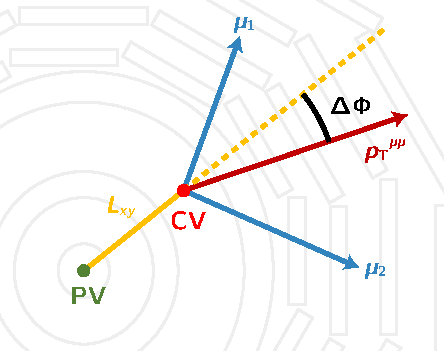
\includegraphics[width=.7\textwidth]{figures/displaced/LxyDef.pdf}
  \caption[Diagram of key variables (\Lxy and \DeltaPhi) used in the analysis.]{Diagram of the key variables used in this analysis. A long-lived particle is produced at the primary vertex (PV) and travels some distance in the detector before decaying into two muons ($\Pgm_1$ and $\Pgm_2$), forming a common vertex (CV). The distance between these two vertices in the transverse plane is referred to as \Lxy, the transverse decay length. The angle between the \Lxy vector and the \pT vector of the dimuon system is referred to as \DeltaPhi, the collinearity angle in the transverse plane.}
  \label{fig:dd:keyvars}
\end{figure}

The quantity \LxySig is referred as the \Lxy significance, as it is a measure of the significance of the fit compared to zero displacement.
For a well-reconstructed dimuon corresponding to a long-lived particle decaying a few tens of centimeters away from the PV, as in signal events, this quantity is large.
On the other hand, background events from reconstruction mistakes or promptly produced particles, such as can arise in Drell-Yan events, are expected to result in dimuons with small \Lxy significance.
A large \Lxy significance is therefore a strong indicator of consistency with the long-lived particle hypothesis.

The collinearity angle in the transverse plane between the dimuon \pT vector ($\pT^{\Pgm\Pgm}$) and the \Lxy vector is referred to as \DeltaPhi.
For a real pair of muons originating from a CV formed from the decay of a long-lived particle originating at the PV, the resulting dimuon momentum vector points towards the PV, and \DeltaPhi is small.
On the other hand, in most types of background events, this quantity is expected to be symmetric around $\pi/2$.
A small \DeltaPhi is therefore a strong indicator of consistency with the long-lived particle hypothesis.

\Fig~\ref{fig:dd:keyvars} illustrates these important quantities and their relationship to each other.

\section{Muon Reconstruction}
This analysis is a search for pairs of muons consistent with originating from a common vertex that is displaced with respect to the beam spot.
Such dimuon vertices can arise from decays of exotic long-lived particles, which are produced promptly (as a direct result of the hard interaction process and produced close to the beam spot) and travel for some distance before decaying.
As mentioned in \Sec~\ref{sec:dd:Trigger}, muons produced from such decays may not point towards the beam spot.
Most algorithms performing the offline reconstruction of muon tracks, however, include the beam spot; these reconstructions are described as being ``updated at the vertex.''
A search for displaced dimuons must therefore use a reconstruction algorithm that does not use this beam spot constraint.

Muons reconstructed using only hits in the muon system are known as standalone muons.
Standalone muons are independent of the more precise information from the silicon tracker, and so have poorer spatial and momentum resolution than muons reconstructed using the tracker.
However, the reconstruction efficiency for tracker tracks with transverse impact parameter $d_0$ (the closest distance between the track and the beam spot in the transverse plane) of more than a few tens of \cm is essentially zero, while the muon system gives non-vanishing reconstruction efficiency even a few meters away from the beam spot.
Therefore, standalone muons are the reconstructed object of choice for a displaced dimuon search sensitive to longer lifetimes.
Furthermore, standalone muon reconstruction is available with and without the beam spot constraint.
Standalone muons without this beam spot constraint are the starting point for choosing a muon reconstruction suitable for studying displaced dimuons.

The analyses performed using Run~1 data used refitted standalone muons (RSA muons) as their primary muon reconstruction \cite{CMS-PAS-EXO-14-012,CMS-AN-14-176}.
Compared to ordinary standalone muons without the beam spot constraint, the RSA muon algorithm computes a final refit (an additional iteration in the standalone muon trajectory builder) excluding the beam spot.
This reconstruction was intended to reduce the inherent bias towards the beam spot exhibited by the standard standalone muon reconstruction designed to study muons originating directly from the \pp collision.
RSA muons thus have improved $d_0$ and \pT resolution compared to standalone muons.

Another muon reconstruction algorithm is the displaced standalone muon (DSA muon) reconstruction.
Compared to ordinary standalone muons without the beam spot constraint, the DSA muon reconstruction is seeded with groups of segments in the muon chambers with criteria similar to those used for the reconstruction of cosmic muons, as opposed to seeds used for the reconstruction of muons originating from \pp collisions \cite{CMS-DP-2015-015}.
This reconstruction was intended to further improve the \pT resolution of muons produced from highly displaced decays.

\Fig~\ref{fig:dd:REFF} shows graphs of the efficiency as a function of generated \Lxy to reconstruct a generated muon as DSA or as RSA, with and without the trigger applied, with respect to \mbox{$\PHiggs\to2\PLLP\to2\Pgm$} signal events in which both generated muons are within a detector acceptance, defined as
\begin{itemize}
  \item both generated muon $\pT > 25\GeV$
  \item both generated muon $|\eta| < 2$
  \item generated \mbox{$\Lxy < 500\cm$}
\end{itemize}
In order to have a sufficient sample size, all 33 of the \twoMu signal samples are combined together for these graphs.
The reconstruction efficiency decreases steadily as a function of generated \Lxy, dropping off sharply at about 600\cm, corresponding roughly to the start of the third barrel muon station, and the DSA reconstruction is consistently higher than the RSA reconstruction.
With the trigger applied, the reconstruction efficiency is high for both DSA and RSA muons, up until about 300\cm at which point the trigger efficiency seriously limits the number of passing events.

\begin{figure}[p]
  \centering
  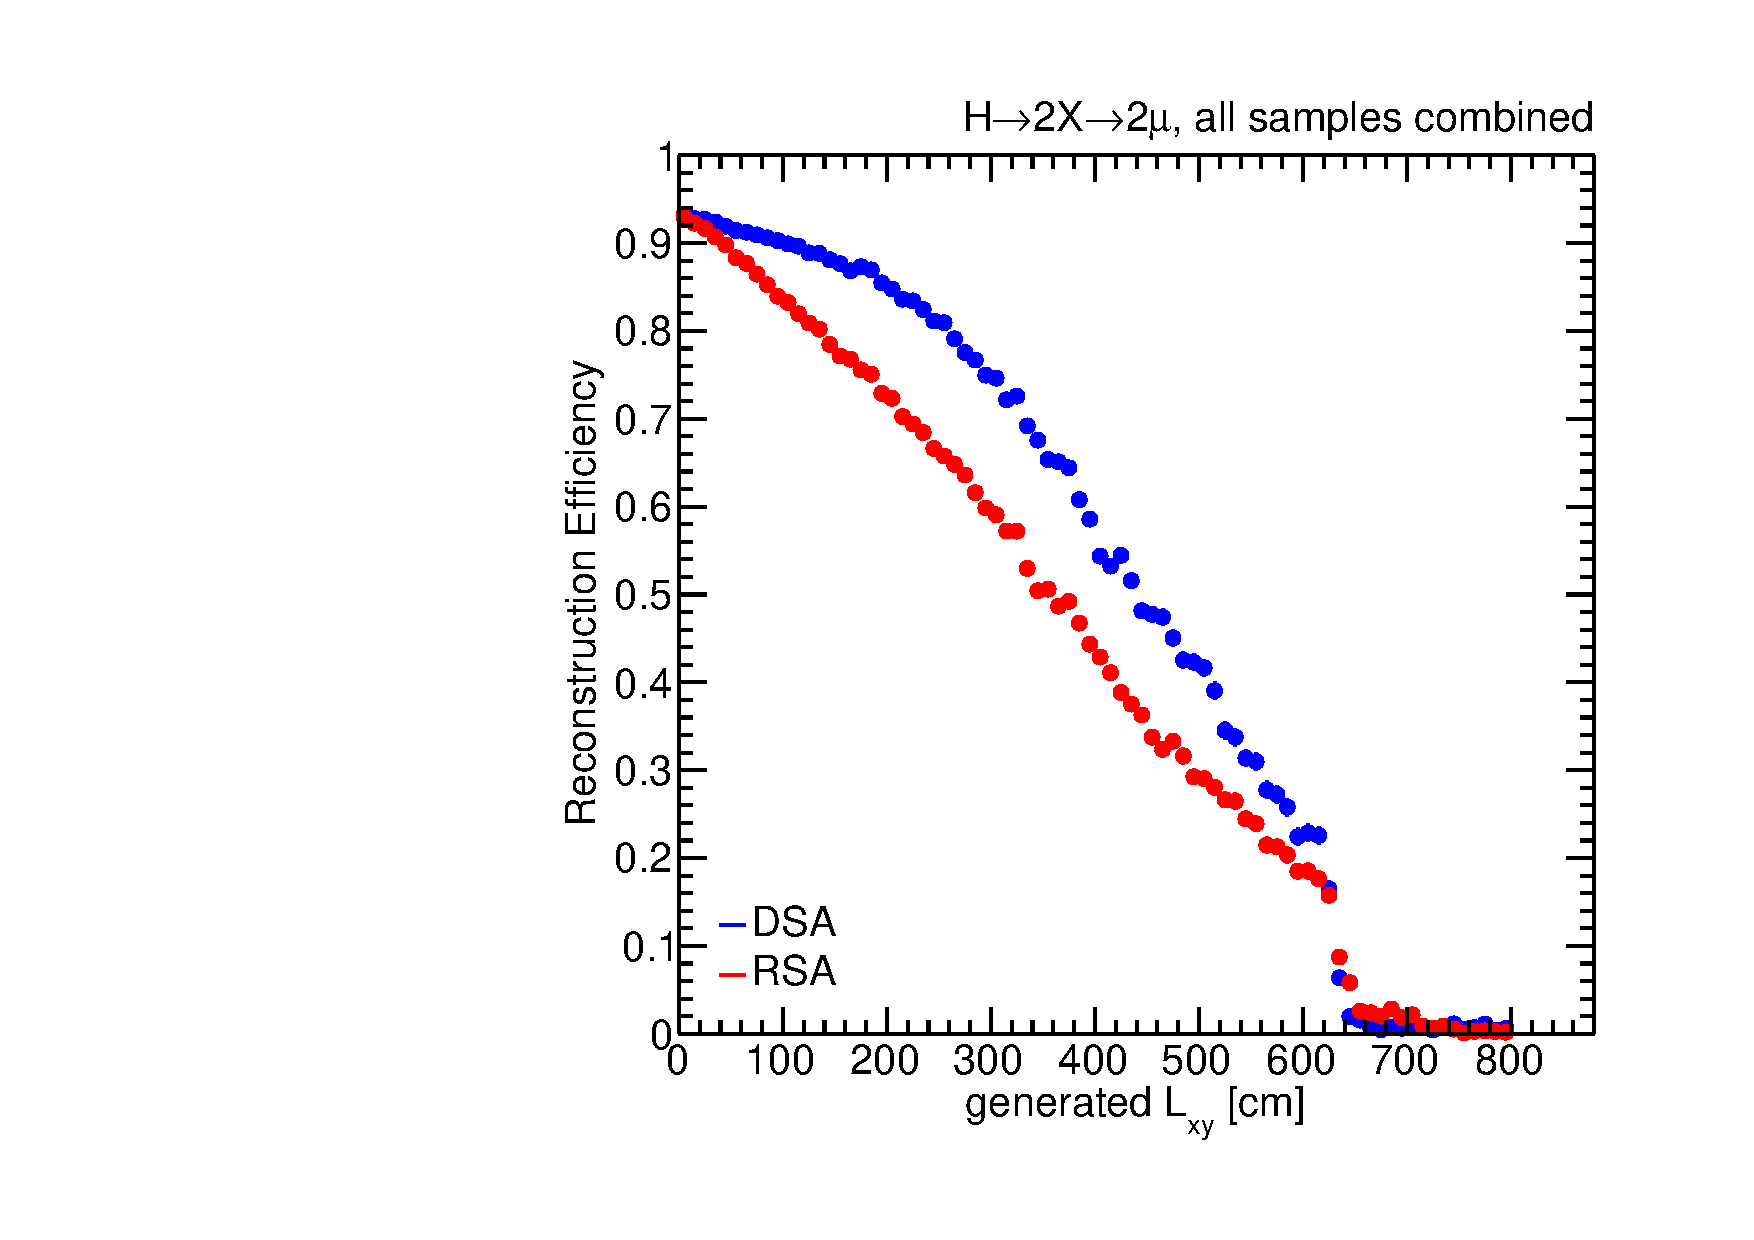
\includegraphics[width=\DSquareWidth]{figures/displaced/REFF_Lxy_2Mu2J_Global.pdf}
  \hspace*{-2em}
  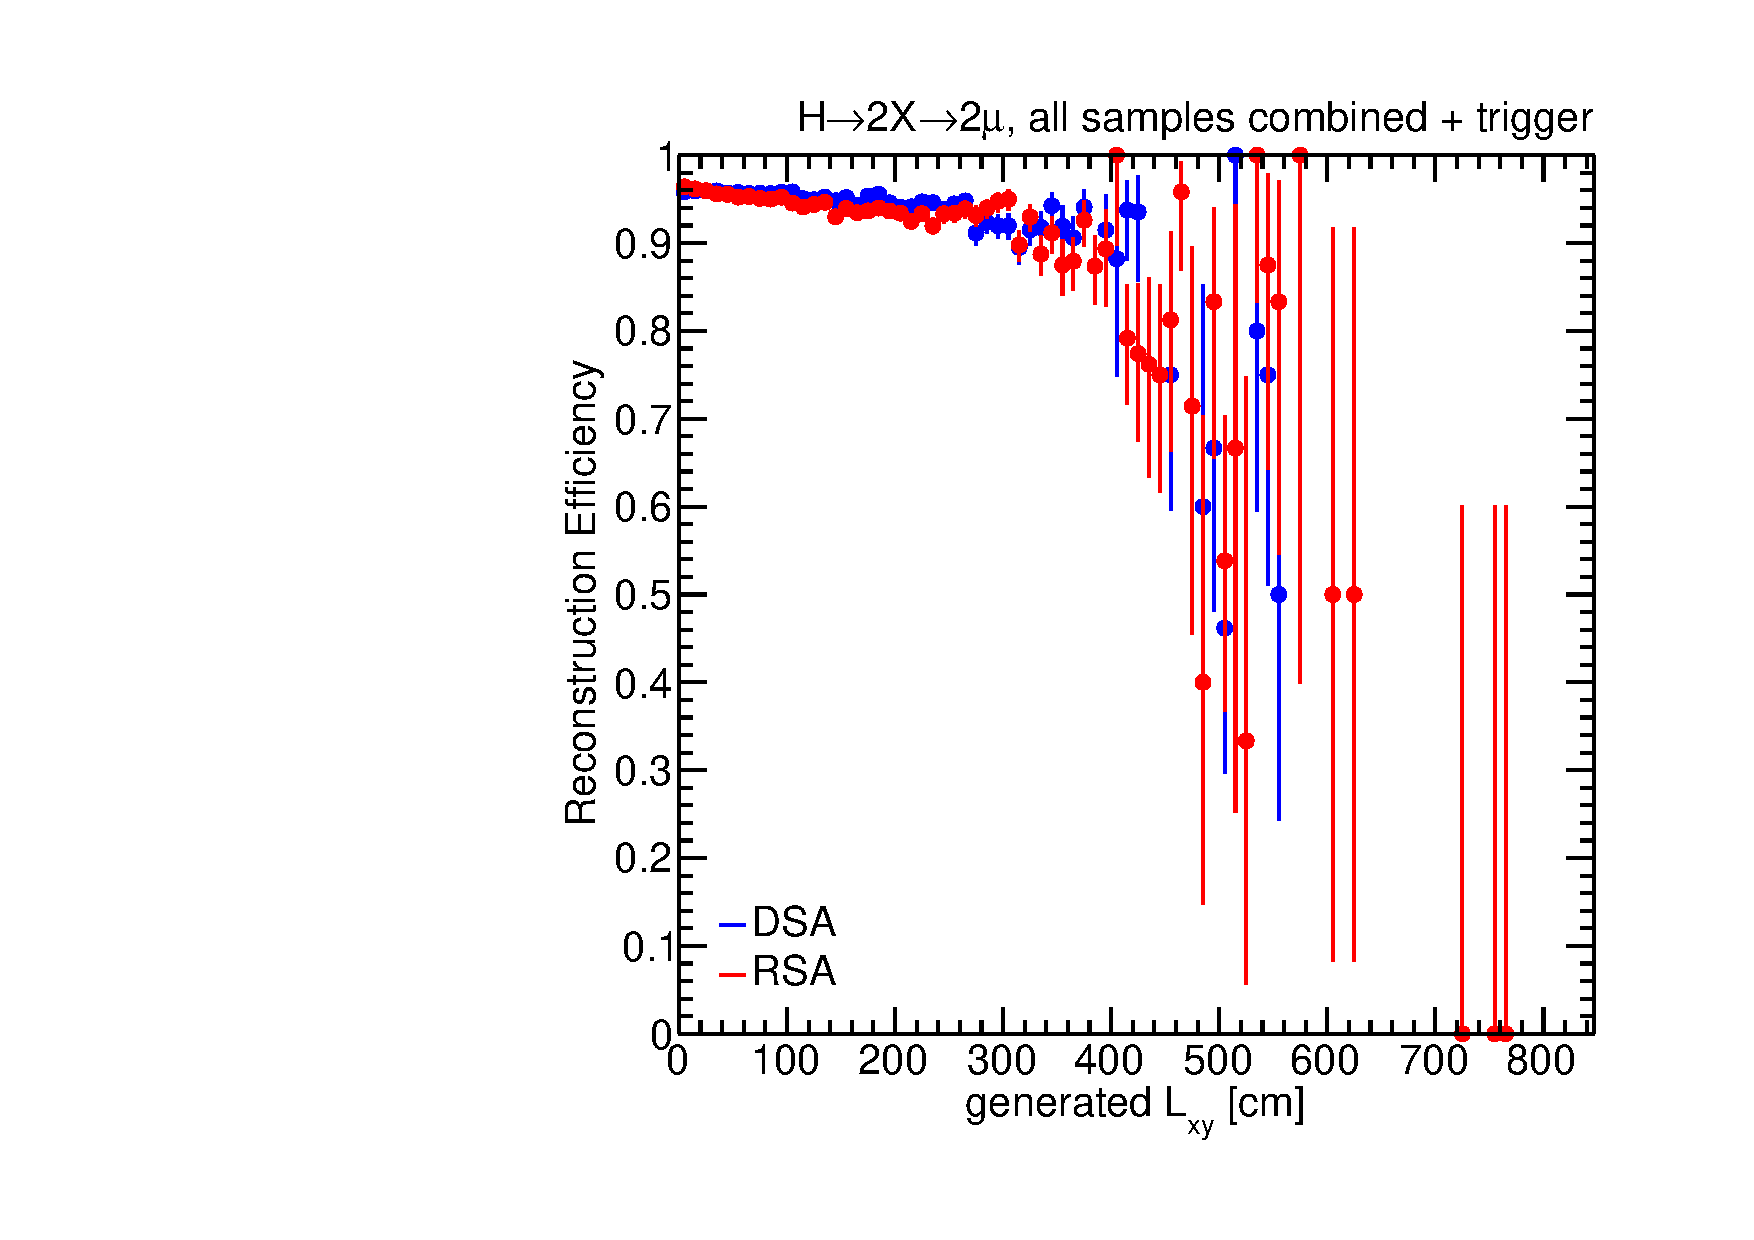
\includegraphics[width=\DSquareWidth]{figures/displaced/REFF_Lxy_Trig_2Mu2J_Global.pdf}
  \caption[DSA and RSA reconstruction efficiency as a function of generated \Lxy]{DSA and RSA reconstruction efficiency as a function of generated \Lxy for \twoMu signal events combining all 33 signal samples, with respect to events within acceptance, \figpos{left} without and \figpos{right} with the trigger applied. Error bars are for statistical uncertainty only.}
  \label{fig:dd:REFF}
\end{figure}
\begin{figure}[p]
  \centering
  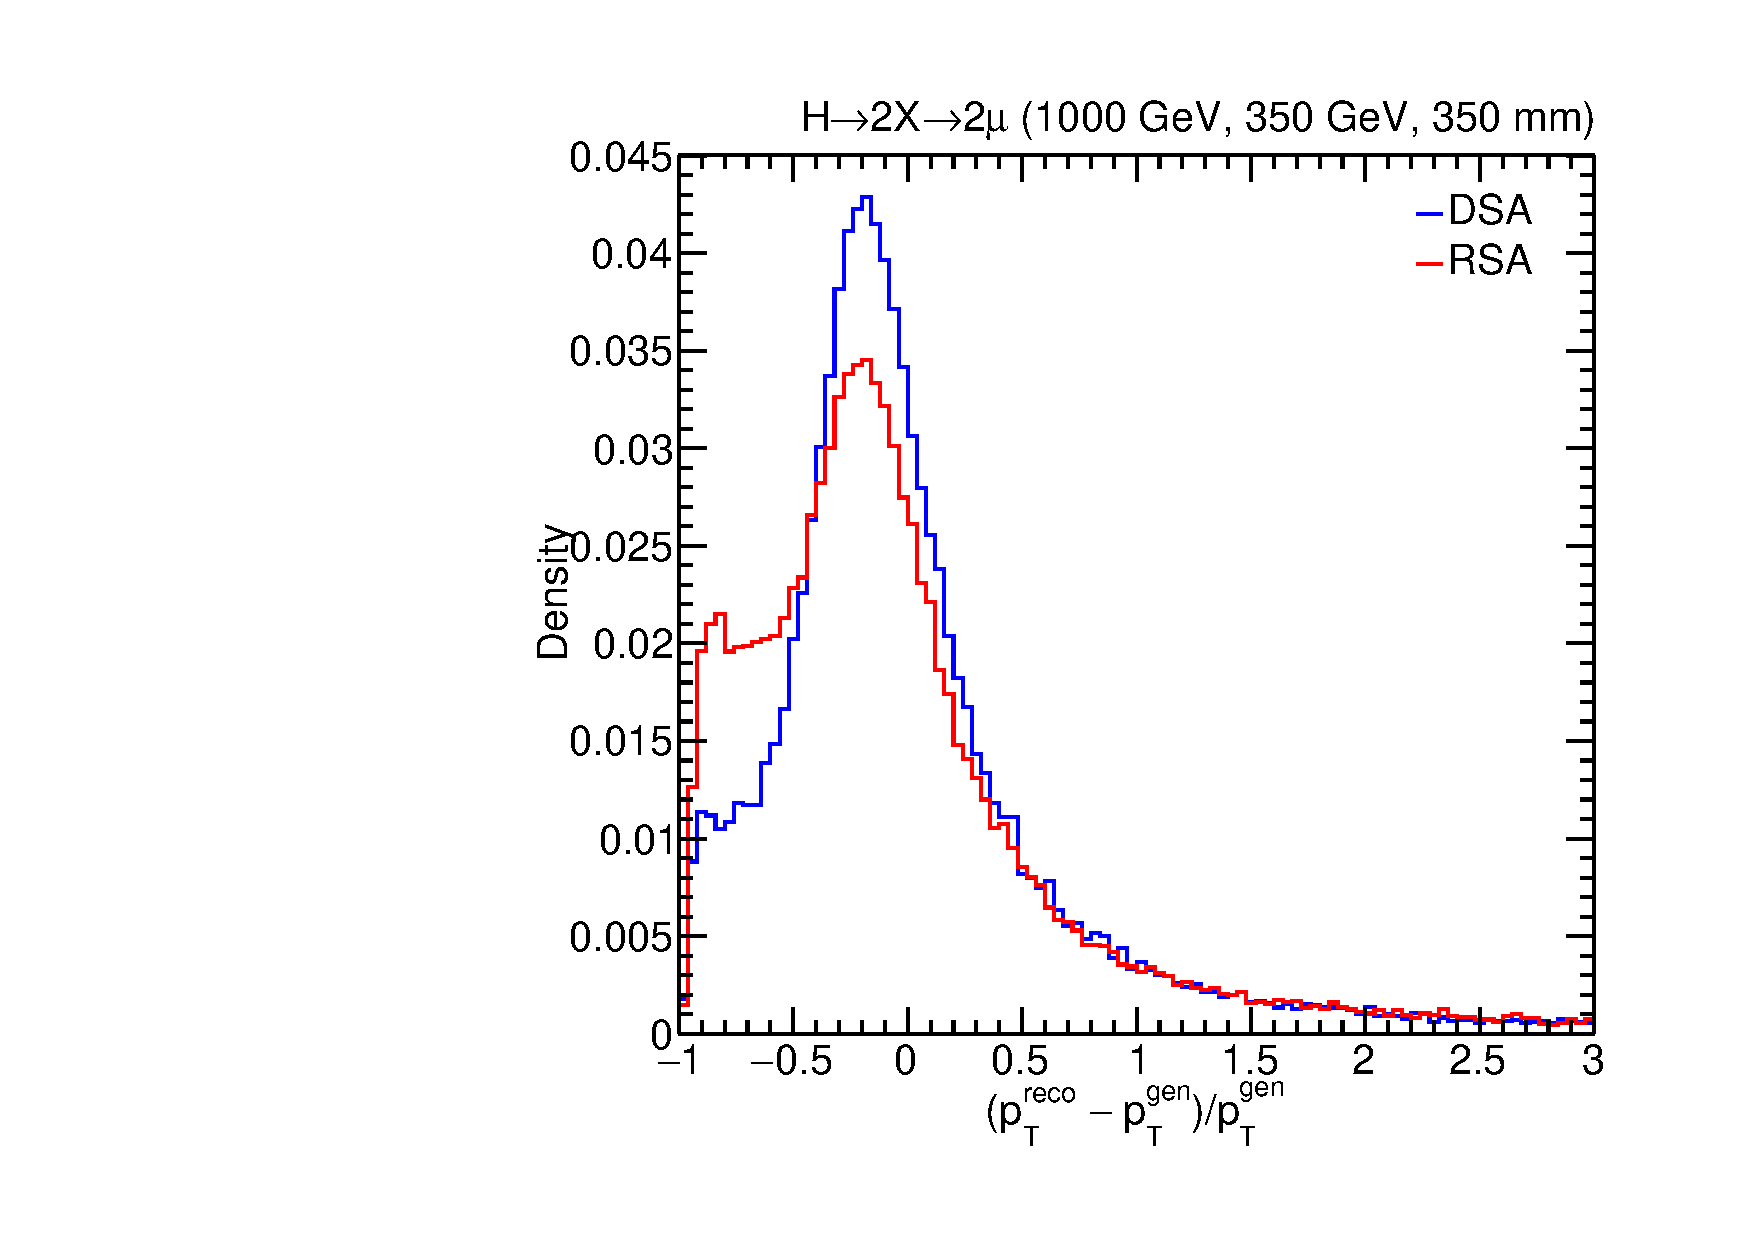
\includegraphics[width=\DSquareWidth]{figures/displaced/PTRES_2Mu2J_1000_350_350.pdf}
  \hspace*{-2em}
  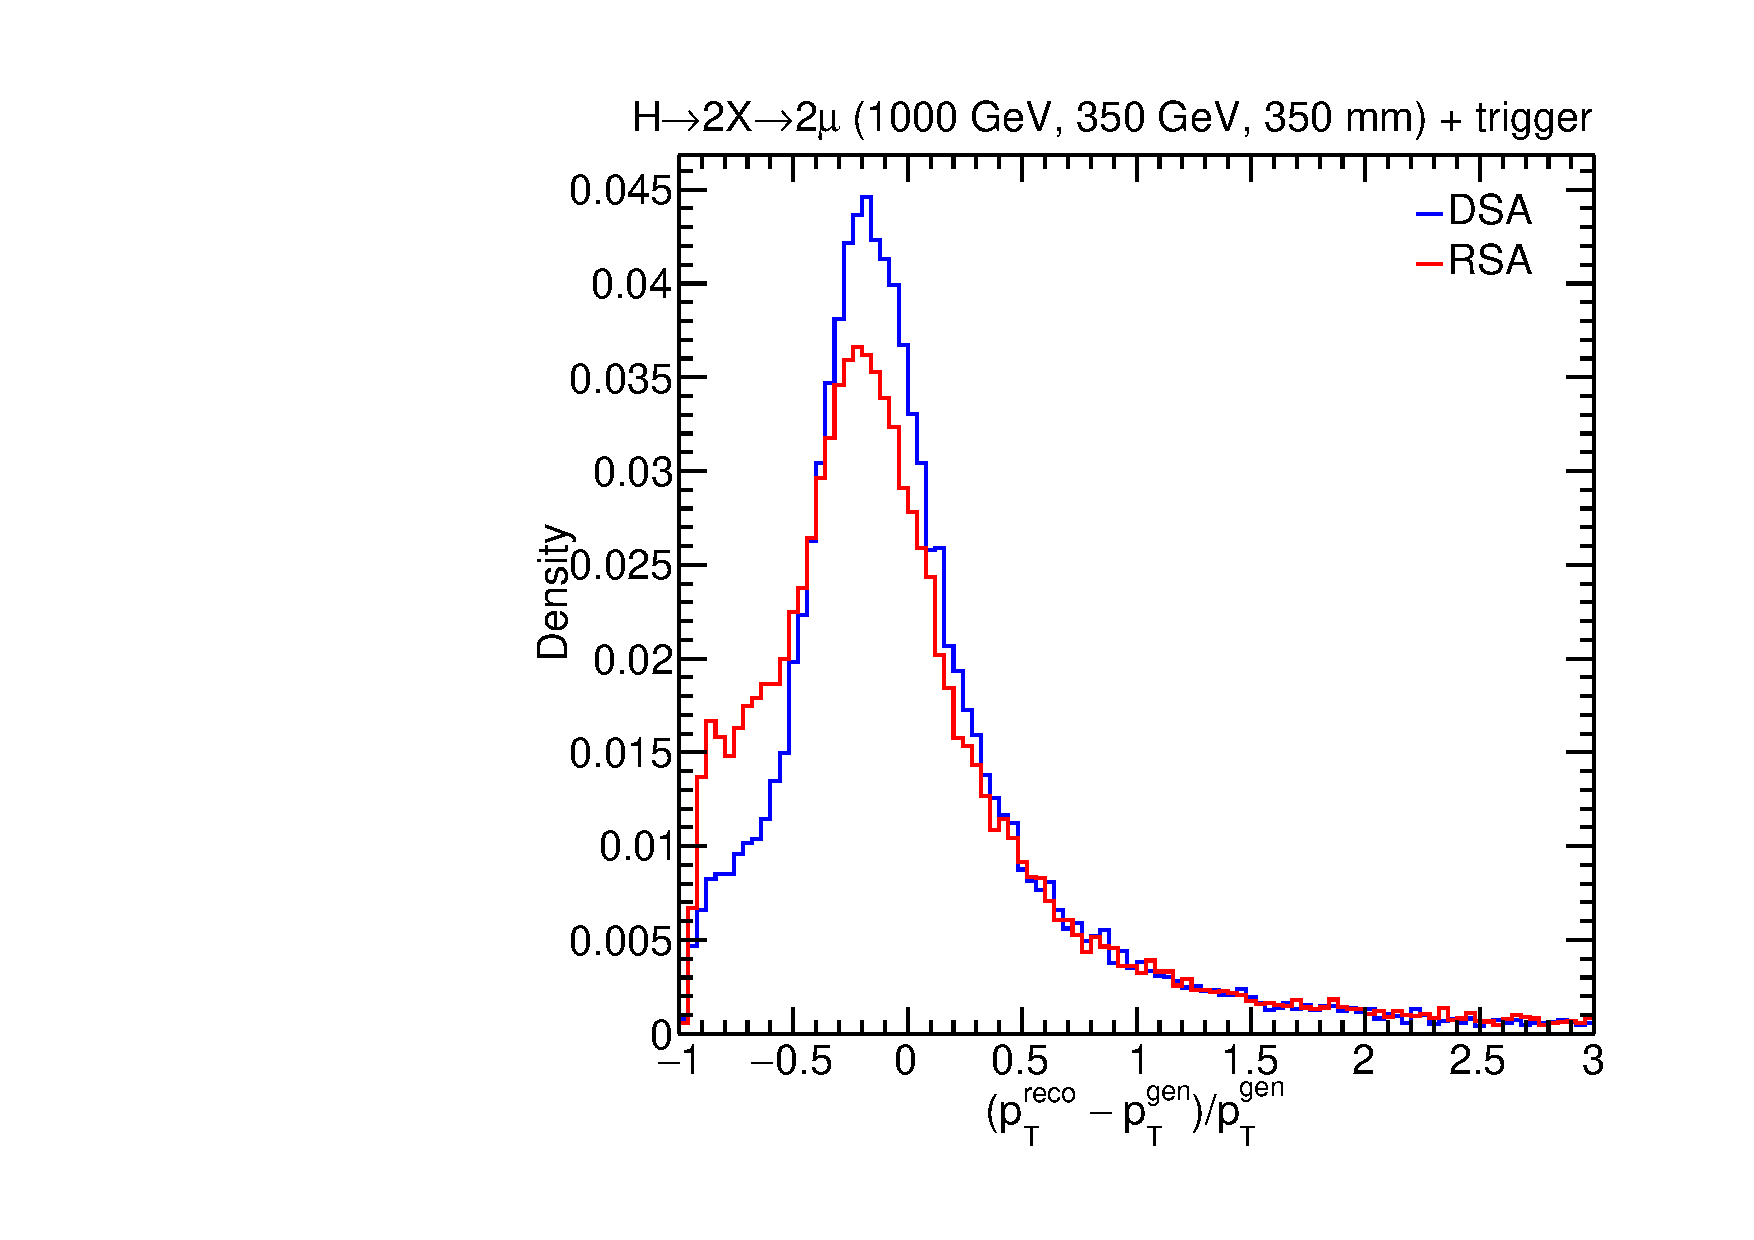
\includegraphics[width=\DSquareWidth]{figures/displaced/PTRES_Trig_2Mu2J_1000_350_350.pdf}
  \caption[DSA and RSA \pT resolution for generated events within acceptance]{DSA and RSA \pT resolution for generated events within acceptance, \figpos{left} without the trigger applied and \figpos{right} with the trigger applied, for the \twoMu signal sample with \FullSP{1000}{350}{350}.}
  \label{fig:dd:PTRES_DSA_RSA}
\end{figure}


\Fig~\ref{fig:dd:PTRES_DSA_RSA} shows distributions of the \pT resolution for the DSA and RSA reconstructions, normalized to unit area, for generated events within acceptance, with and without the trigger applied, for the \twoMu signal sample with \FullSP{1000}{350}{350}.
The RSA reconstruction gives a visibly worse \pT resolution, with a larger shoulder near $-1$, indicating that RSA muons tend to underestimate the muon \pT compared to DSA muons.

\Figs~\ref{fig:dd:REFF}--\ref{fig:dd:PTRES_DSA_RSA} show that DSA muons have both a higher reconstruction efficiency and an improved \pT resolution over RSA muons.
The analysis presented in this thesis therefore primarily uses DSA muons.

\section{Event and Object Selection}
\subsection{Overview}
\label{sec:dd:GeneralStrategy}
An overview of the general strategy for selecting reconstructed events and objects consistent with displaced dimuons is as follows.
\clearpage
\begin{enumerate}
  \item \textbf{DSA muon preselection}. Begin with DSA muons as seeds for searching for displaced dimuons and apply a set of quality criteria to select muons that are reasonably well reconstructed. (\Sec~\ref{sec:dd:DSAQuality})
  \item \textbf{HLT-RECO matching}. Keep only events that contain offline reconstructed muons that match the online trigger muons passing the HLT. (\Sec~\ref{sec:dd:HLTMatching})
  \item \textbf{\DSAToPAT muon association}. Attempt to associate DSA muons with global or arbitrated tracker muons (referred to as PAT muons, named after the \textbf{P}hysics \textbf{A}nalysis \textbf{T}ools in the CMS software that process them), and if they can be, replace the DSA muons with the associated PAT muons. This analysis focuses on the DSA muons that are \emph{not} associated with PAT muons, so this step essentially sets aside DSA muons that are consistent with muons reconstructed using the tracker. (\Sec~\ref{sec:dd:Association})
  \item \textbf{DSA muon object selection}. Apply additional selections to remaining DSA muons that identify DSA muons in signal-like events and ensure that they are of good quality. (\Sec~\ref{sec:dd:DSAObject})
  \item \textbf{Dimuon formation from common vertex fit}. Form dimuons by fitting two DSA muon tracks to a common vertex. (\Sec~\ref{sec:dd:DimVertex})
  \item \textbf{Pairing criteria}. Select the 1--2 dimuons most likely to be signal dimuons according to a set of muon pairing criteria. (\Sec~\ref{sec:dd:PC})
  \item \textbf{Dimuon object selection}. Apply additional selections to dimuons that identify dimuons in signal-like events and ensure they are of good quality. (\Sec~\ref{sec:dd:DimuonObject})
  \item \textbf{Dimuon signal selection}. Apply additional selections to dimuons that require the dimuon be displaced from the beam spot and have a form consistent with the signal hypothesis that the dimuon originates from the decay of a long-lived particle into two oppositely-charged muons. (\Sec~\ref{sec:dd:DimuonSignal})
  \item \textbf{Cosmic muon suppression}. Apply additional requirements to suppress background events from cosmic muons. (\Sec~\ref{sec:dd:CosmicCuts})
\end{enumerate}

\subsection{DSA Muon Preselection}
\label{sec:dd:DSAQuality}
Event and object preselection begins with DSA muons.
The HLT path described in \Sec~\ref{sec:dd:Trigger} reconstructs muons at Level~2 using a procedure similar to that used to reconstruct muons as refitted standalone (RSA) muons at the offline reconstructed level.
However, as discussed in the previous section, DSA muons are chosen as the starting point over RSA muons for their improved \pT resolution and higher reconstruction efficiency.
DSA muons are required to satisfy the following quality criteria:
\begin{itemize}
  \item reconstructed with hits in at least two muon stations, \ie $$N(\text{CSC stations}) + N(\text{DT stations}) > 1$$
  \item reconstructed with at least 13 hits in the muon stations, \ie $$N(\text{CSC hits}) + N(\text{DT hits}) > 12$$
  \item relative \pT uncertainty of less than 100\%, \ie $$\pTErr/\pT < 1$$
\end{itemize}

These quality criteria ensure that the DSA muons have acceptable \pT resolution and charge assignment.
\Fig~\ref{fig:dd:QCUT_PTRES} shows distributions of the DSA muon \pT resolution for the \twoMu signal sample with \FullSP{1000}{350}{350} for events split up by the $N_\text{hits}$ cut and for events split up by the $\pTErr/\pT$ cut, each population normalized to unit area.
The events satisfying the cut have reasonable \pT resolution, while the events failing the cut have rather poor \pT resolution.
\Fig~\ref{fig:dd:QCUT_QDIFF} shows distributions of the difference between reconstructed and generated charge for the same signal sample, for events split up by the $N_\text{hits}$ cut and for events split up by the $\pTErr/\pT$ cut, each population normalized to unit area.
The events satisfying the cut are assigned the correct charge in more than 90\% of events, while the events failing the cut are assigned the correct charge in only around 60\% of events.

\begin{figure}[htpb]
  \centering
  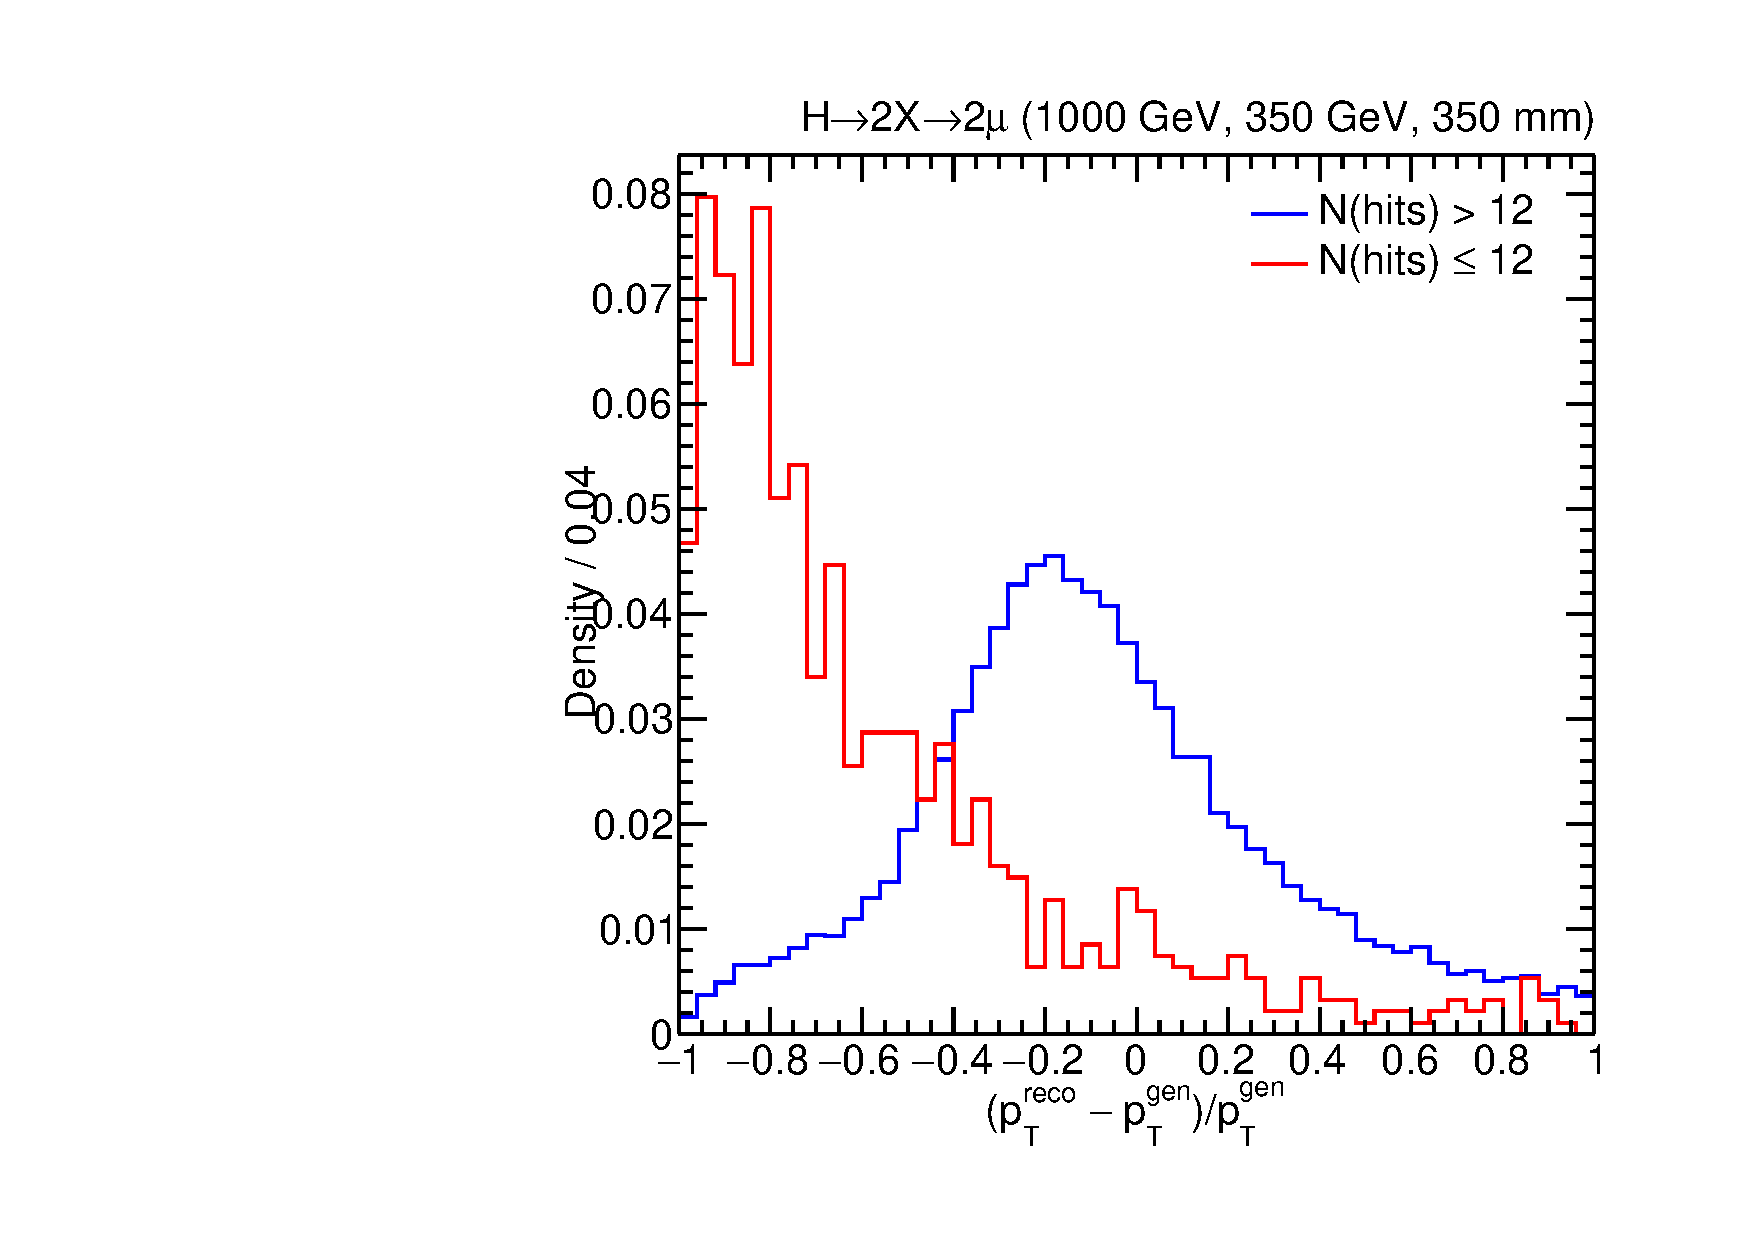
\includegraphics[width=\DSquareWidth]{figures/displaced/QCUTRES_Sig_pTRes_hits_1000_350_350.pdf}
  \hspace*{-2em}
  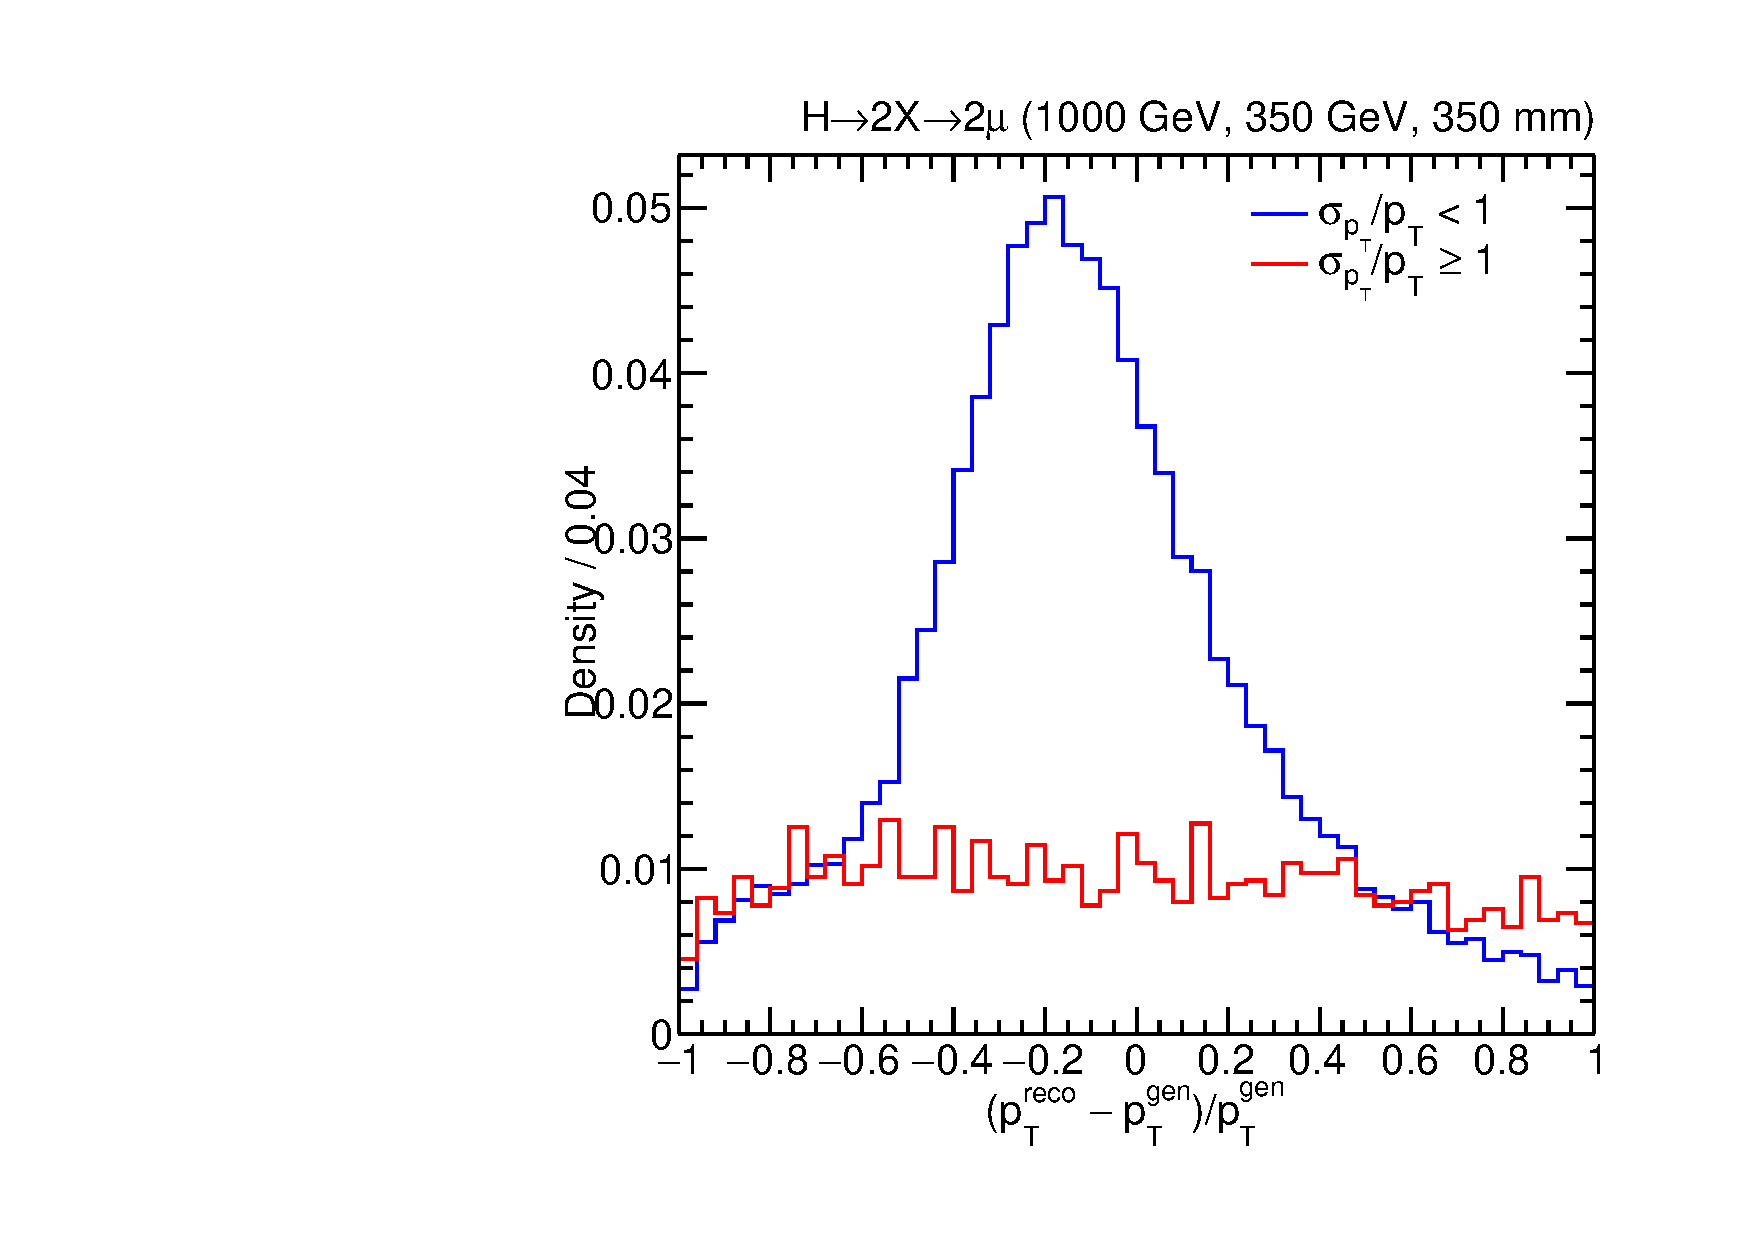
\includegraphics[width=\DSquareWidth]{figures/displaced/QCUTRES_Sig_pTRes_fpte_1000_350_350.pdf}
  \caption[DSA muon \pT resolution with and without selections on $N_\text{hits}$ and $\pTErr/\pT$.]{DSA muon \pT resolution, normalized to unit area, for the \twoMu signal sample with \FullSP{1000}{350}{350} for \figpos{left} events with $N_\text{hits} > 12$ and $N_\text{hits} \leq 12$ separately, and \figpos{right} events with $\pTErr/\pT \geq 1$ and $\pTErr/\pT < 1$ separately.}
  \label{fig:dd:QCUT_PTRES}
\end{figure}
\begin{figure}[htpb]
  \centering
  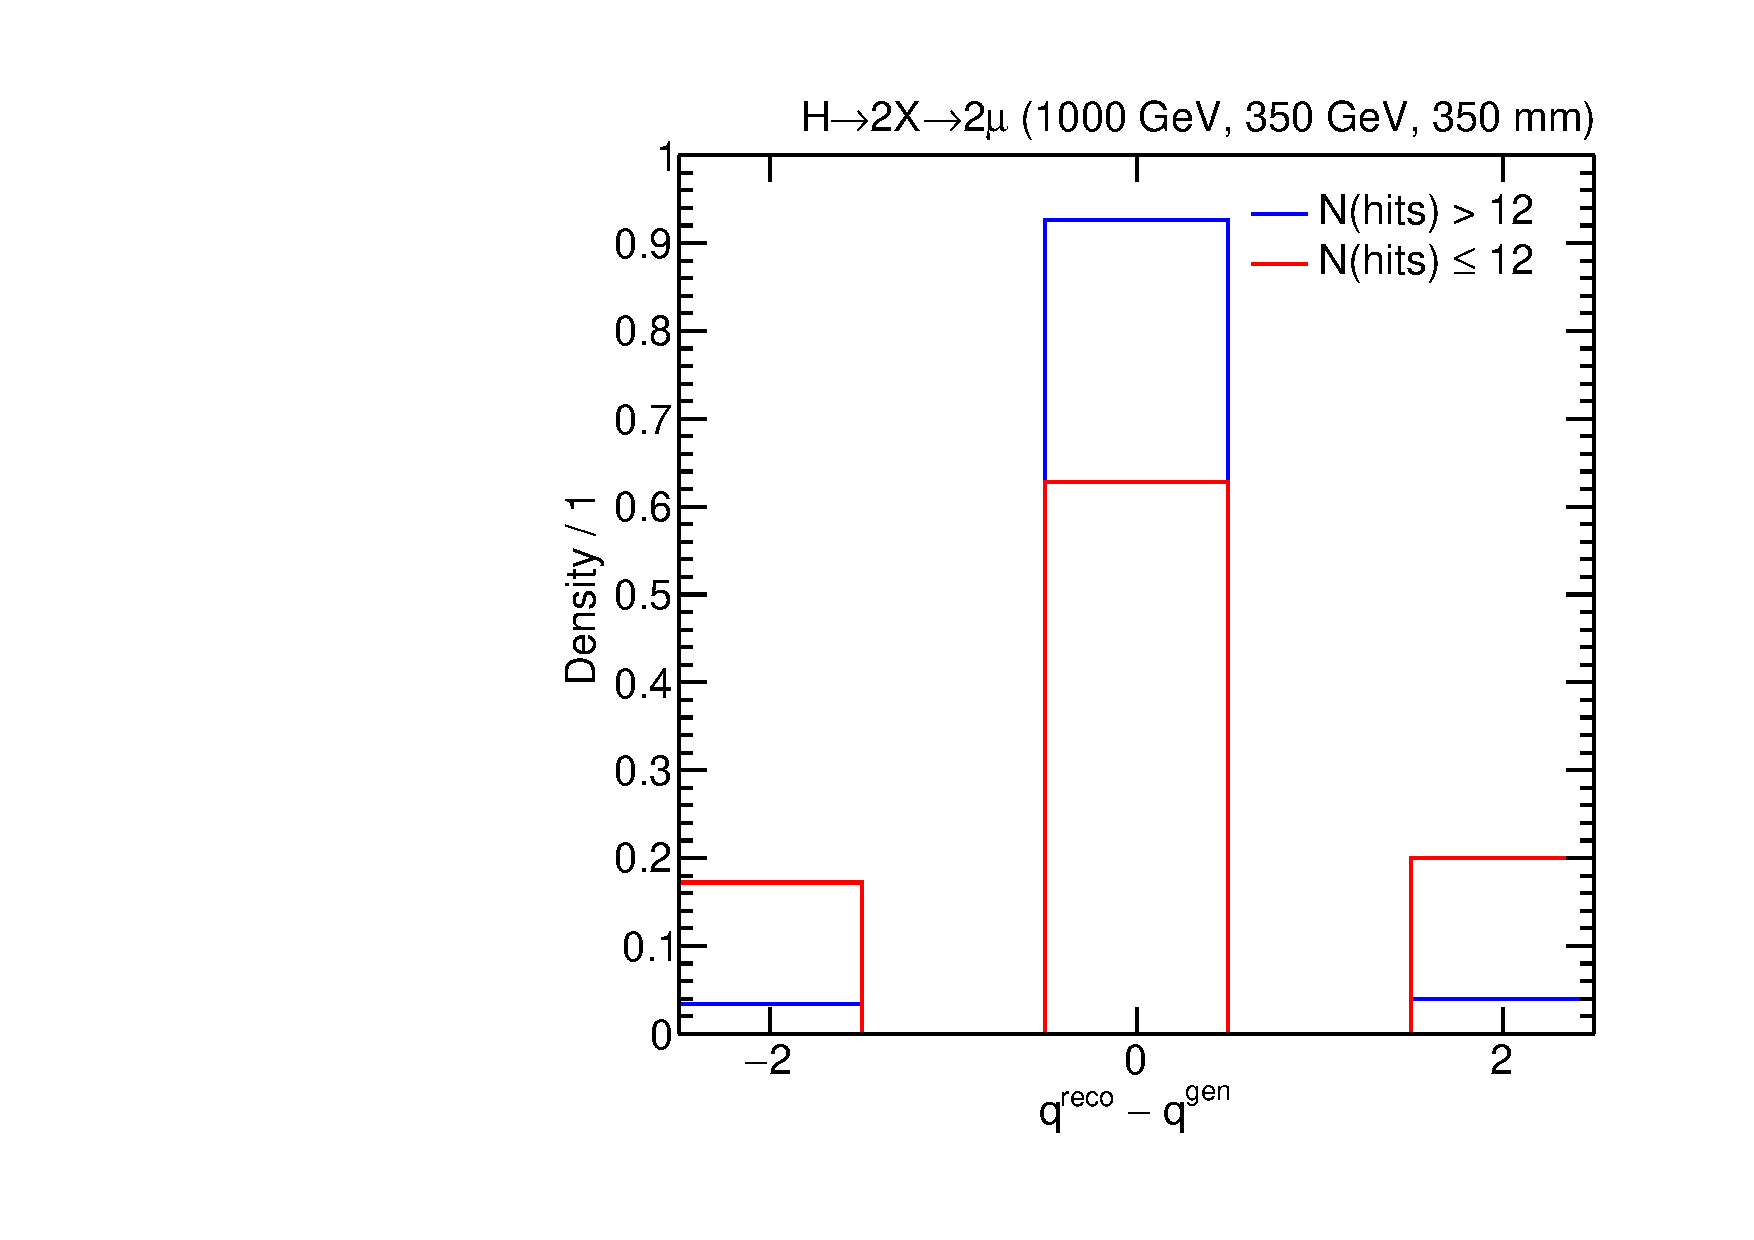
\includegraphics[width=\DSquareWidth]{figures/displaced/QCUTRES_Sig_qdiff_hits_1000_350_350.pdf}
  \hspace*{-2em}
  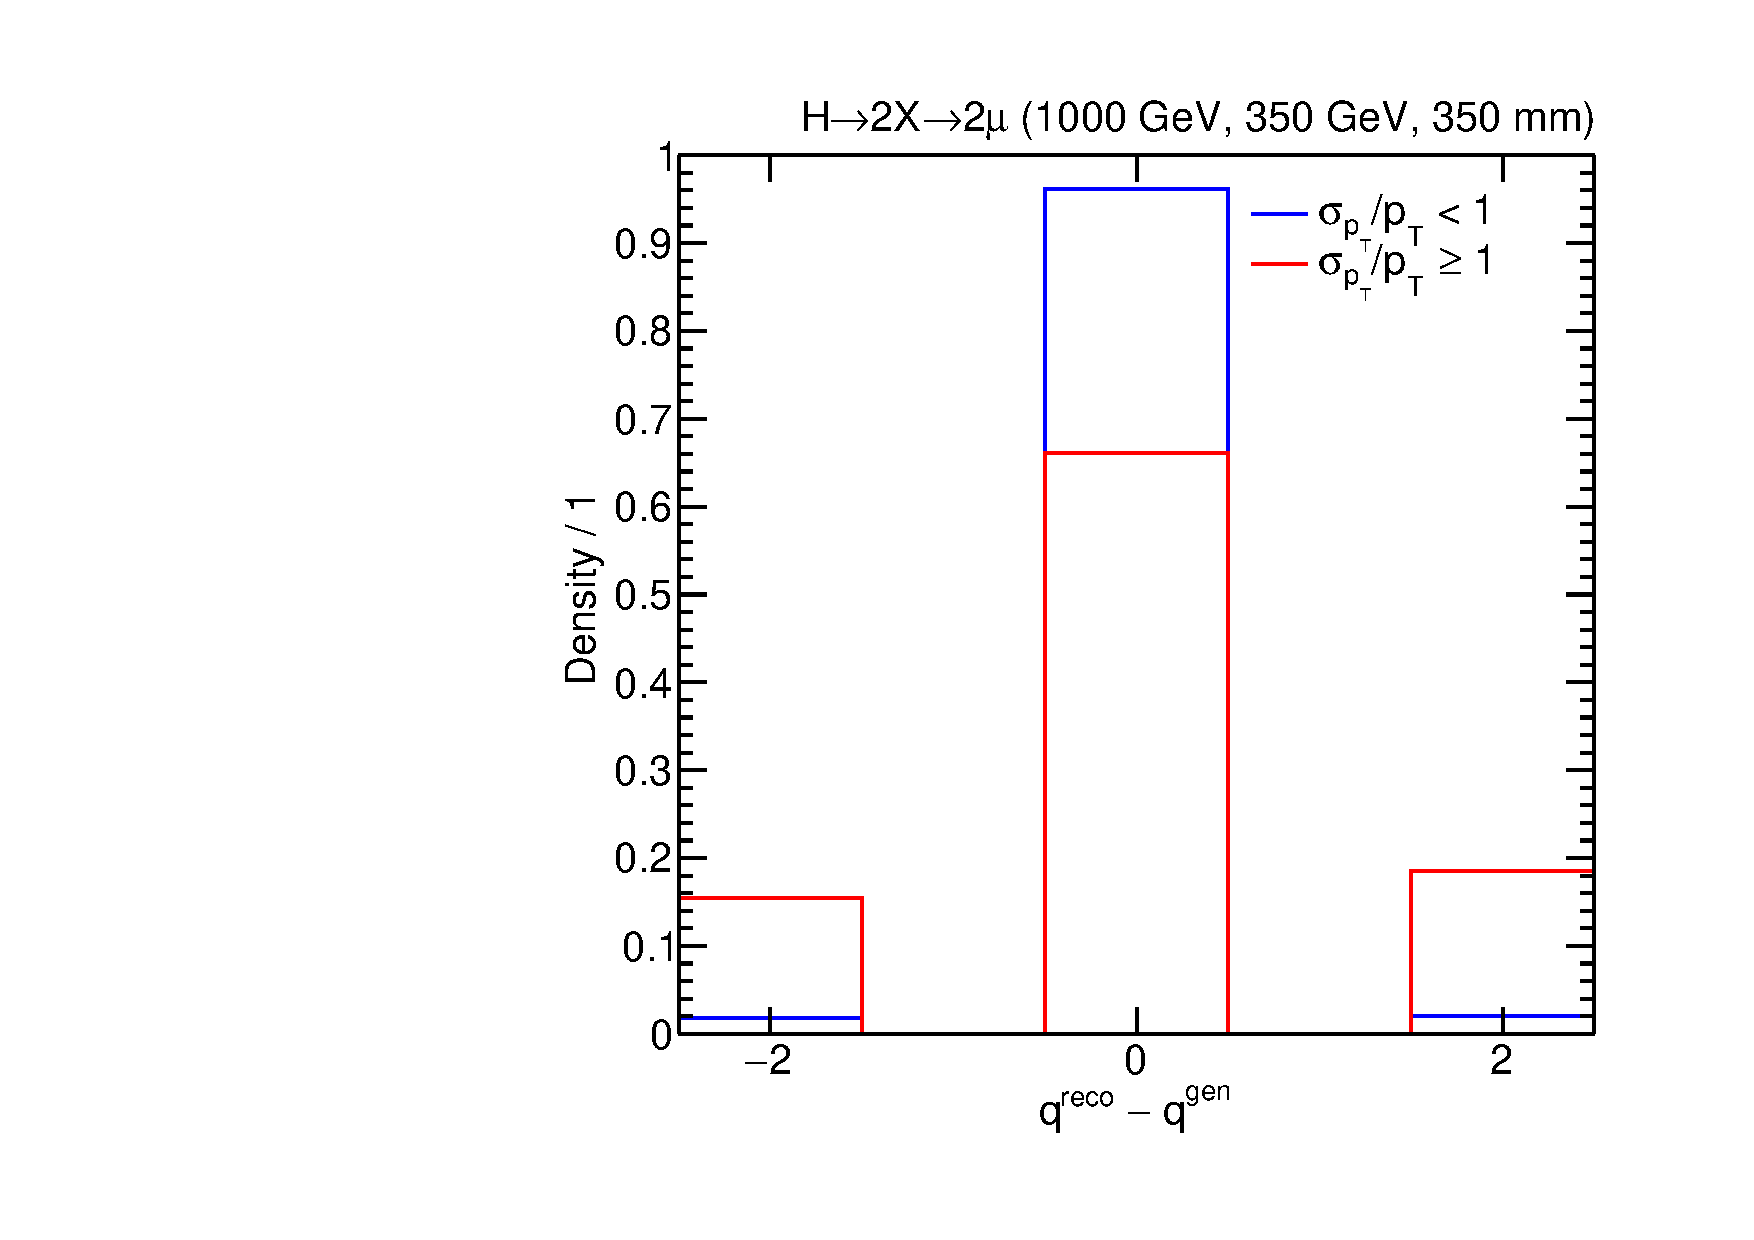
\includegraphics[width=\DSquareWidth]{figures/displaced/QCUTRES_Sig_qdiff_fpte_1000_350_350.pdf}
  \caption[DSA muon charge difference with and without selections on $N_\text{hits}$ and $\pTErr/\pT$.]{DSA muon charge difference, normalized to unit area, for the \twoMu signal sample with \FullSP{1000}{350}{350} for \figpos{left} events with $N_\text{hits} > 12$ and $N_\text{hits} \leq 12$ separately, and \figpos{right} events with $\pTErr/\pT \geq 1$ and $\pTErr/\pT < 1$ separately.}
  \label{fig:dd:QCUT_QDIFF}
\end{figure}

\subsection{HLT-RECO Matching}
\label{sec:dd:HLTMatching}
Next, only events in which the HLT decision is matched using the preselected DSA muons are kept, in a procedure referred to as HLT-RECO matching.
This ensures that the quickly-reconstructed, coarser-resolution muons reconstructed by the trigger system have counterparts among muons reconstructed offline using the higher-precision data of the full event.
For the purposes of HLT-RECO matching, DSA muons are required to pass loose \pT and $\eta$ requirements: $\pT > 10\GeV$ and $|\eta| < 2.0$.
These DSA muons are referred to as DSA muons for trigger matching.
Let \deltaR refer to the angular proximity in $\eta$-$\phi$ space between two three-vectors, defined as
\begin{equation}
  \Delta R = \sqrt{\left(\Delta\eta\right)^2 + \left(\Delta\phi\right)^2}
  \label{eq:dd:deltaR}
\end{equation}
Then HLT-RECO matching requires that each of the pair of distinct DSA muons for trigger matching lie within cones of $\deltaR < 0.4$ around each muon among pairs of muons reconstructed at Level~2 passing the trigger (HLT muons).

The \pT, $\eta$, and \deltaR requirements are all chosen to empirically optimize the trade-off between efficiency and purity, matching as many events as possible while keeping the frequency of accidental matches to poor quality muons low.
The HLT-RECO matching procedure retains more than 98\% of \twoMu signal events that passed the trigger and have at least two DSA muons for trigger matching.

The HLT-RECO matching requirement ensures, at the event level, that the trigger decision is confirmed using objects reconstructed offline.
The subsequent object selection, however, does not require that selected dimuons be formed from pairs of triggering HLT muons.
This allows the analysis to be sensitive to \fourMu final states, in which two of the four muons passed the trigger, but all four muons are signal muons.

\subsection{\DSAToPAT Muon Association}
\label{sec:dd:Association}
This analysis begins with DSA muons to identify potential displaced muon events, specifically focusing on highly displaced events in which the long-lived particle travels far enough before decaying that a track is not observed in the tracker.
Implementing this requirement necessitates development of a procedure to efficiently associate DSA muons with muons reconstructed using the tracker.
This association improves not only potential signal discrimination, but also background rejection.
Ensuring that this procedure is both highly efficient (\ie muons that should be associated, are) and highly pure (\ie muons that should not be associated, are not) requires some care.
This section describes the details of the association procedure.

\subsubsection{PAT Muons and Matching Criteria}
Offline reconstructed muons having either of the following properties are considered:
\begin{itemize}
  \item \textbf{Global muons}. Global muons are muons reconstructed by association a tracker track with a standalone muon by collecting all the hits from both and performing a full track fit, called a global muon fit. Global muons are the primary muon reconstruction used by most CMS analyses.
  \item \textbf{Arbitrated tracker muons}. In order to deal with cases in which global muon reconstruction is inefficient, tracker muons were developed. Tracker muons do not require a standalone muon; instead, a tracker track is extrapolated and associated with hits in the muon system. In the case of multiple tracker tracks associated with the same muon hits, an algorithm called arbitration chooses which association to prefer such that no two tracker muons share muon segments; these tracker muons are referred to as arbitrated tracker muons.
\end{itemize}
The muons considered in this analysis that are reconstructed offline using both the tracker and the muon system are referred to as PAT muons.
(PAT is an abbreviation for \textbf{P}hysics \textbf{A}nalysis \textbf{T}ools, a toolkit that is part of the CMS software and which is used to process event and object reconstruction.)
A PAT muon may be both a global muon and an arbitrated tracker muon, and good quality PAT muons are often both.

Candidate PAT muons are associated with DSA muons when they satisfy one of two matching criteria, which are applied in different contexts in a procedure described below. The two matching criteria are:
\begin{itemize}
  \item \textbf{Segment-matched}: A PAT muon is segment-matched to a DSA muon if the PAT muon shares all of its muon system segments with at least 2/3 of the muon system segments used to reconstruct the DSA muon. PAT muon segments and DSA muon segments are compared coordinate by coordinate for equality and are considered the same if their coordinates match.
  \item \textbf{Proximity-matched}: A PAT muon is proximity-matched to a DSA muon if the \deltaR between
    \begin{itemize}
      \item the position vector of the innermost hit of the DSA muon and
      \item the position vector of the point of closest approach of the PAT muon helically extrapolated (in the magnetic field) to the innermost hit of the DSA muon.
    \end{itemize}
    is less than 0.4, with tighter requirements applied in the procedure described below.
\end{itemize}

The proximity match is defined as it is above because DSA muons are sometimes reconstructed with an incorrect $\eta$ coordinate, and would not pass a more standard angular proximity match between the momentum directions of the DSA and PAT muons.
The helical extrapolation and comparison between the positions improved the efficiency of the proximity match.

\subsubsection{\DSAToPAT Association Procedure}
The general procedure is as follows: given a DSA muon, associate segment-matched PAT muons with the DSA muon, using additional criteria to disambiguate among multiple segment-matched PAT muons.
These additional disambiguation criteria include requiring that segment-matched PAT muons are also the PAT muon with the smallest proximity-match \deltaR (as defined above) and/or requiring that segment-matched muons be global and that they be reconstructed from hits in at least 7 tracker layers.
If no PAT muons segment-match the DSA muon, the smallest-\deltaR proximity-matched PAT muon is associated with the DSA muon if its proximity-match \deltaR is sufficiently small; the threshold is 0.4 if the proximity-matched PAT muon is global and has the same numbers of muon system hits as the DSA muon, and 0.1 otherwise.
The full technical details of the procedure are depicted in \Fig~\ref{fig:dd:repdiagram}.

\begin{figure}[p]
  \centering
  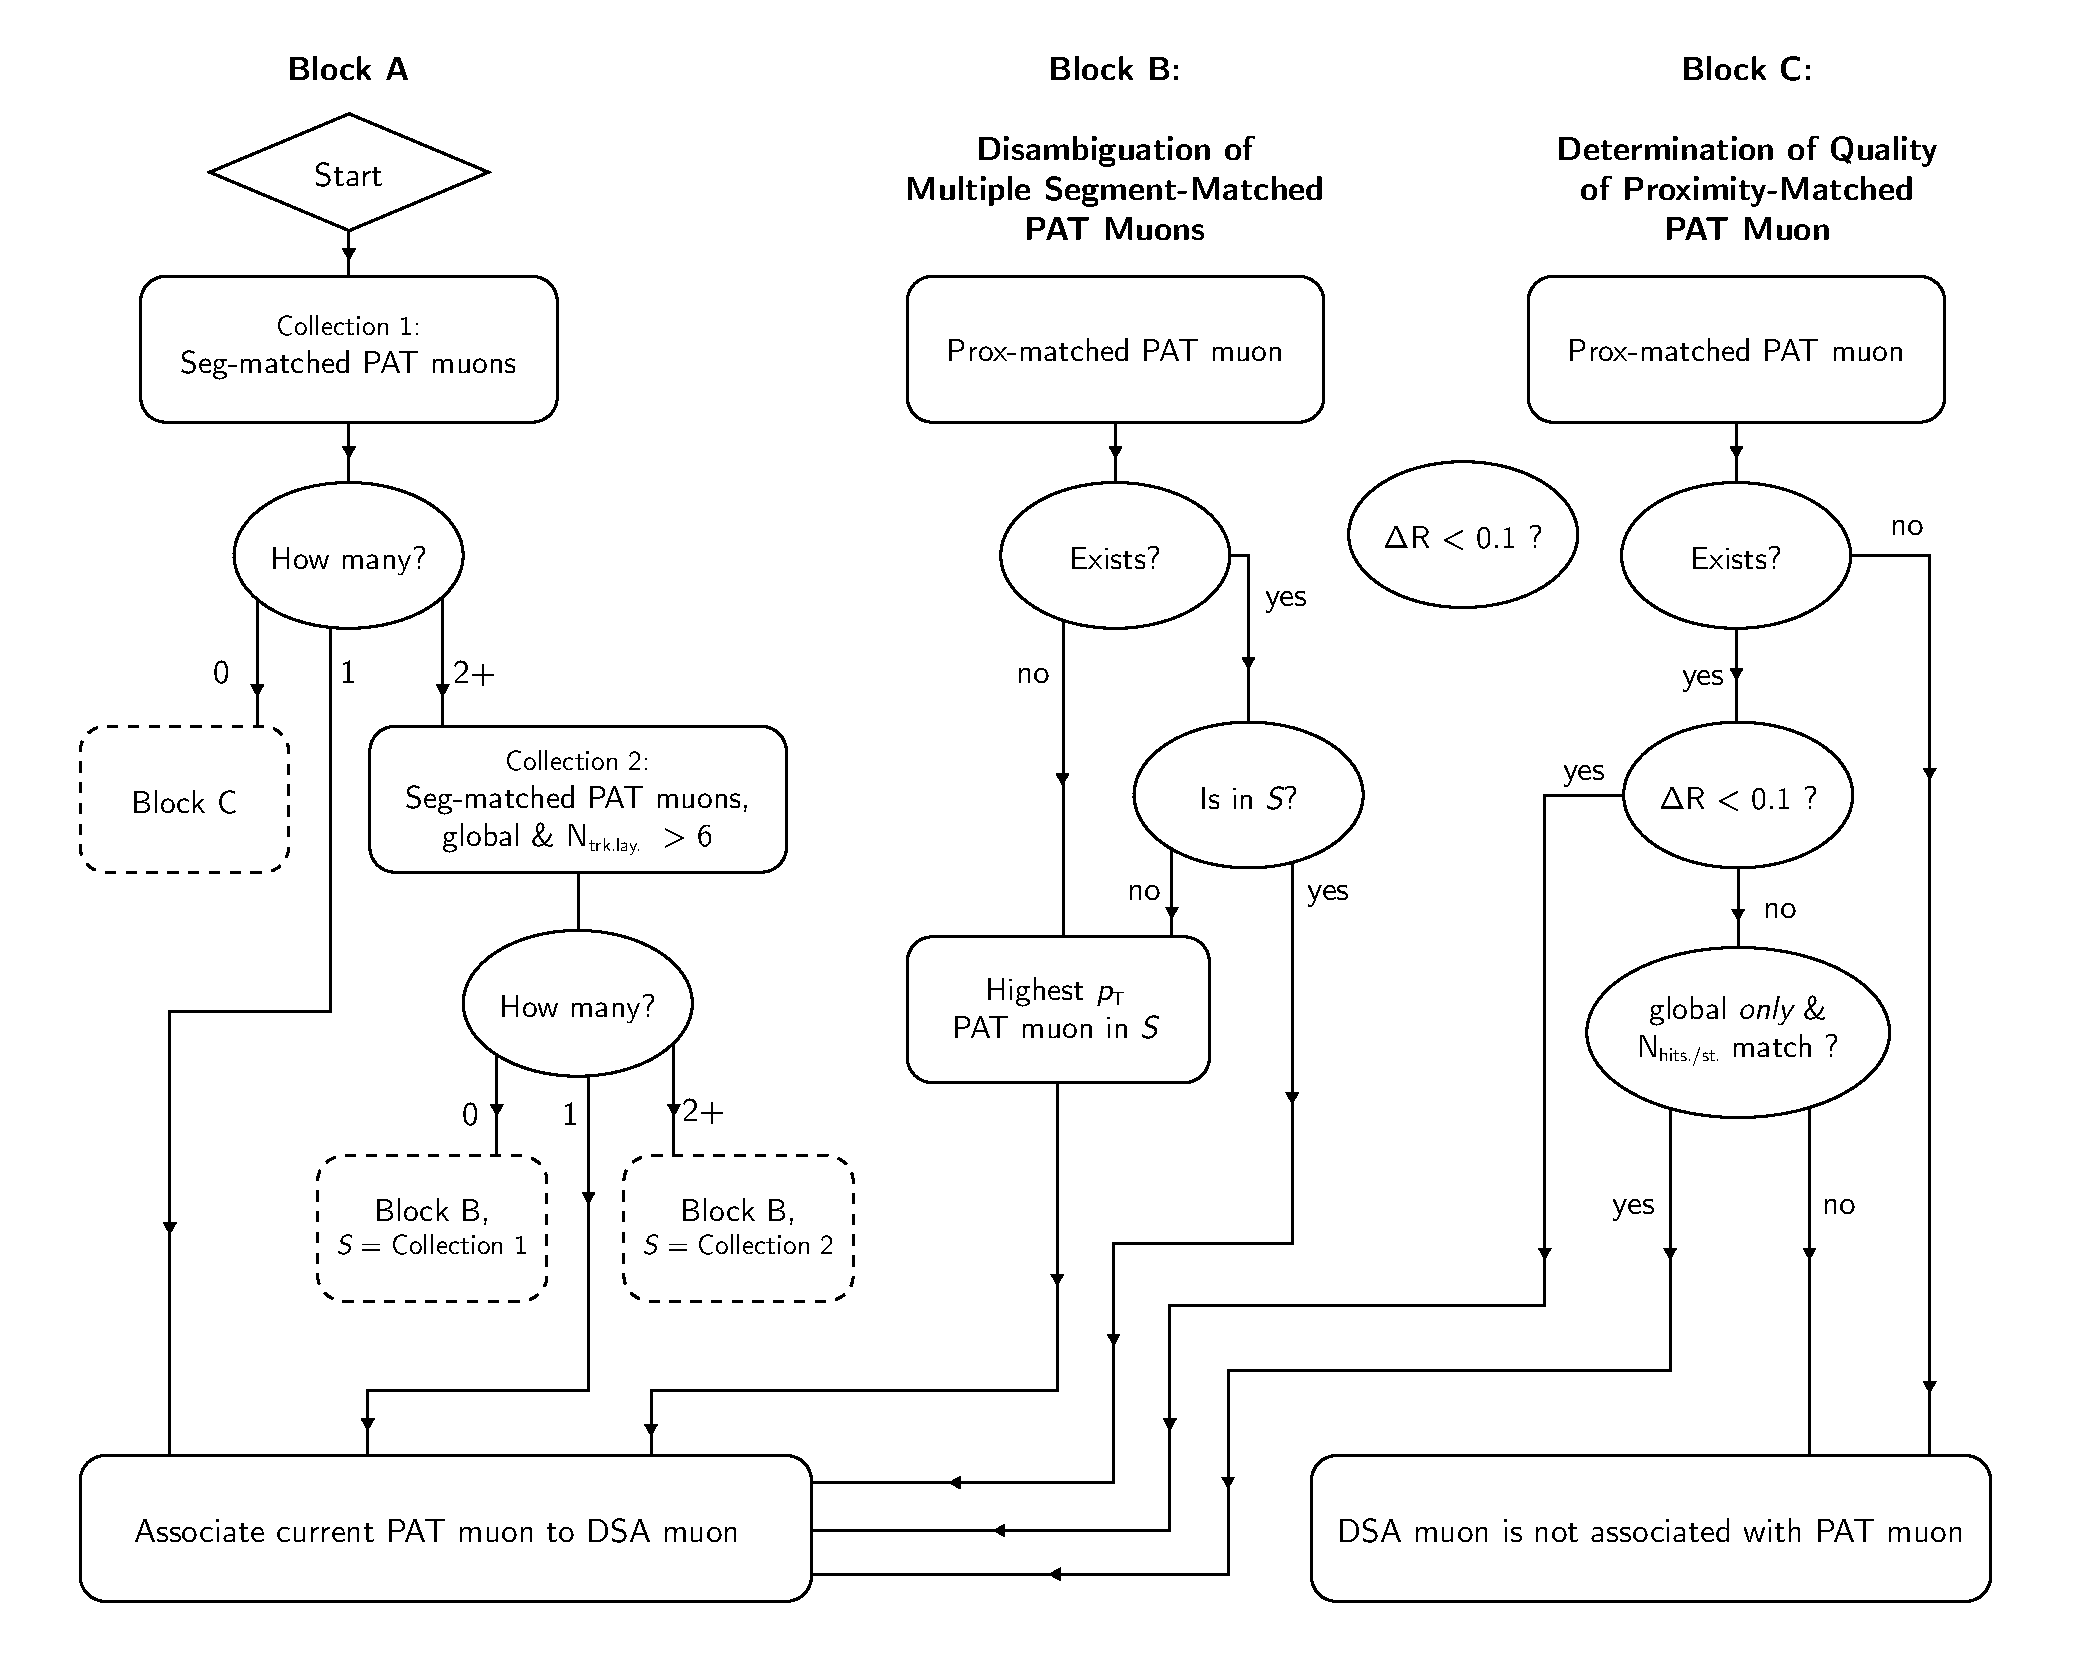
\includegraphics[width=\textwidth]{figures/displaced/ReplacementDiagram.pdf}
  \caption[Flowchart depicting the technical details of the \DSAToPAT association procedure]{Flowchart depicting the technical details of the \DSAToPAT association procedure. The procedure begins by considering segment-matched PAT muons. If there are multiple segment-matched PAT muons, then some temporary quality cuts are applied: the requirements that the muon be global and that it be reconstructed from at least 7 tracker layers (abbreviated $N_\text{trk. lay.}$). When there are multiple segment matches, the PAT muon that has the smallest proximity-match \deltaR is used to disambiguate between them, if possible. If there are no segment matches, then the proximity-matched PAT muon is taken as the match if its proximity \deltaR is sufficiently small. This threshold is 0.4 if the PAT muon is global only (not tracker) and its numbers of CSC and DT hits and stations (abbreviated $N_\text{hits./st.}$) matches those of the DSA muon exactly, and 0.1 otherwise.}
  \label{fig:dd:repdiagram}
\end{figure}

This procedure prioritizes segment-matched PAT muons over proximity-matched PAT muons.
Several combinations of criteria are used to determine the quality selection used to disambiguate segment-matched PAT muons; the combination used here (global and number of tracker layers) is found to be optimal in terms of increasing the efficiency to match to the correct PAT muon.
In principle, there exists the case that a proximity-matched PAT muon does not exist or is not among the segment-matched PAT muons.
In this case, we were prepared to fall back to associating to the highest-\pT PAT muon among the collection of segment-matched PAT muons.
However, this situation never actually occurs in practice.

The \deltaR threshold in the case that there are no segment-matched PAT muons is chosen empirically to increase the matching efficiency while keeping the rate of false, accidental matches low.
At the time of this writing, this analysis does not access the muon system segments used to reconstruct the standalone muons used to form global muons, and so a PAT muon that is global only cannot be segment-matched to a DSA muon.
This has little practical effect on the efficiency to correctly associate DSA muons with PAT muons in this analysis.
For the small fraction of PAT muons that are global only and should be associated with a DSA muon, the proximity-matched PAT muon is often the correct choice.
Therefore, the \deltaR threshold for proximity-matched global-only PAT muons is set at 0.4, if their numbers of CSC and DT hits and stations are identical to those of the DSA muon.
As missed matches can lead to a high rate of background events which are potentially dangerous, this association procedure is also designed to be liberal in order to reject background events: if a DSA muon can be reasonably associated with a PAT muon, it should be, even at the cost of a few accidental matches.
Therefore, in the case of no segment-matched PAT muons and a proximity-matched PAT muon that is a tracker muon, the procedure associates with the DSA muon the proximity-matched PAT muon if its proximity \deltaR is less than 0.1 as a final compromise between efficiency and purity.

As mentioned in \Sec~\ref{sec:dd:mcsamples}, the analysis presented in this thesis focuses only on the DSA muons that are not associated with PAT muons.
To this end, DSA muons are replaced with any associated PAT muons, and so the association step effectively functions as a rejection of DSA muons that can be associated with PAT muons.
The effect of this is that this analysis, using DSA muons, does not benefit from the improved resolution of PAT muons, but it benefits tremendously from the superior background rejection.
This is the analysis sensitive to the longest lifetimes, with long-lived particles decaying in the outer region of the tracker and outside the tracker through the muon system.

The PAT association procedure is highly effective in suppressing \pp collision backgrounds, such as those modeled by the simulated background samples.
\Figs~\ref{fig:dd:REPEFF_MC_LxySig}--\ref{fig:dd:REPEFF_MC_Lxy} are histograms of dimuon \LxySig and \Lxy in simulated background samples, with each process scaled to its equivalent luminosity as discussed in \Sec~\ref{sec:dd:EqLumi}, before and after the association procedure.
The PAT association suppresses events in simulated background by a factor of $10^5$, reducing the number of dimuons from 12.5 million to 204.
For these histograms, a \pT cut of 10\GeV is applied to DSA muons on top of the preselection criteria.
This is a requirement that is part of the muon object selection (see \Sec~\ref{sec:dd:DSAObject}), but is applied here to more clearly demonstrate the effect of the PAT association procedure by suppressing secondary, low-\pT muons not associated with PAT muons, such as those from other \pp collisions in the bunch crossing.

\begin{figure}[p]
  \centering
  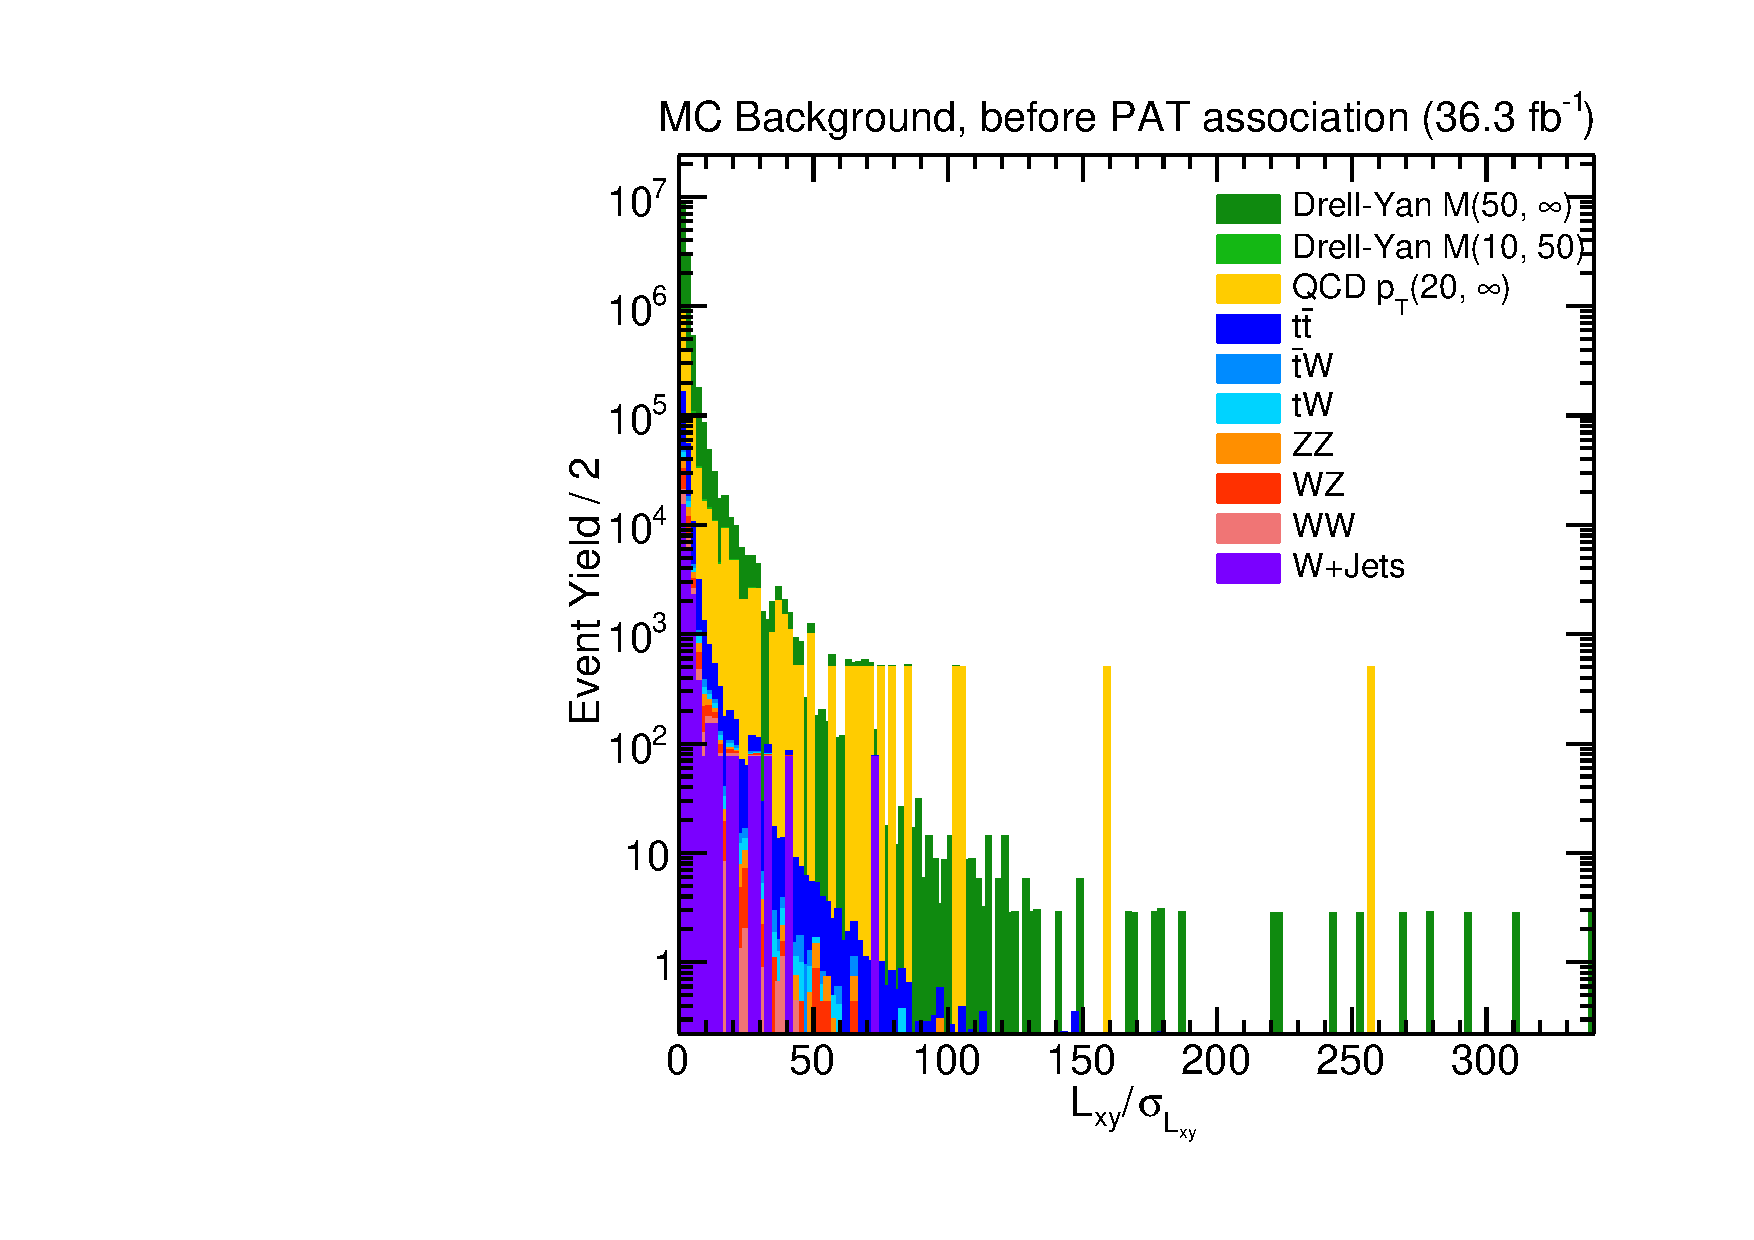
\includegraphics[width=\DSquareWidth]{figures/displaced/REPEFF_MC_LxySig-before.pdf}
  \hspace*{-2em}
  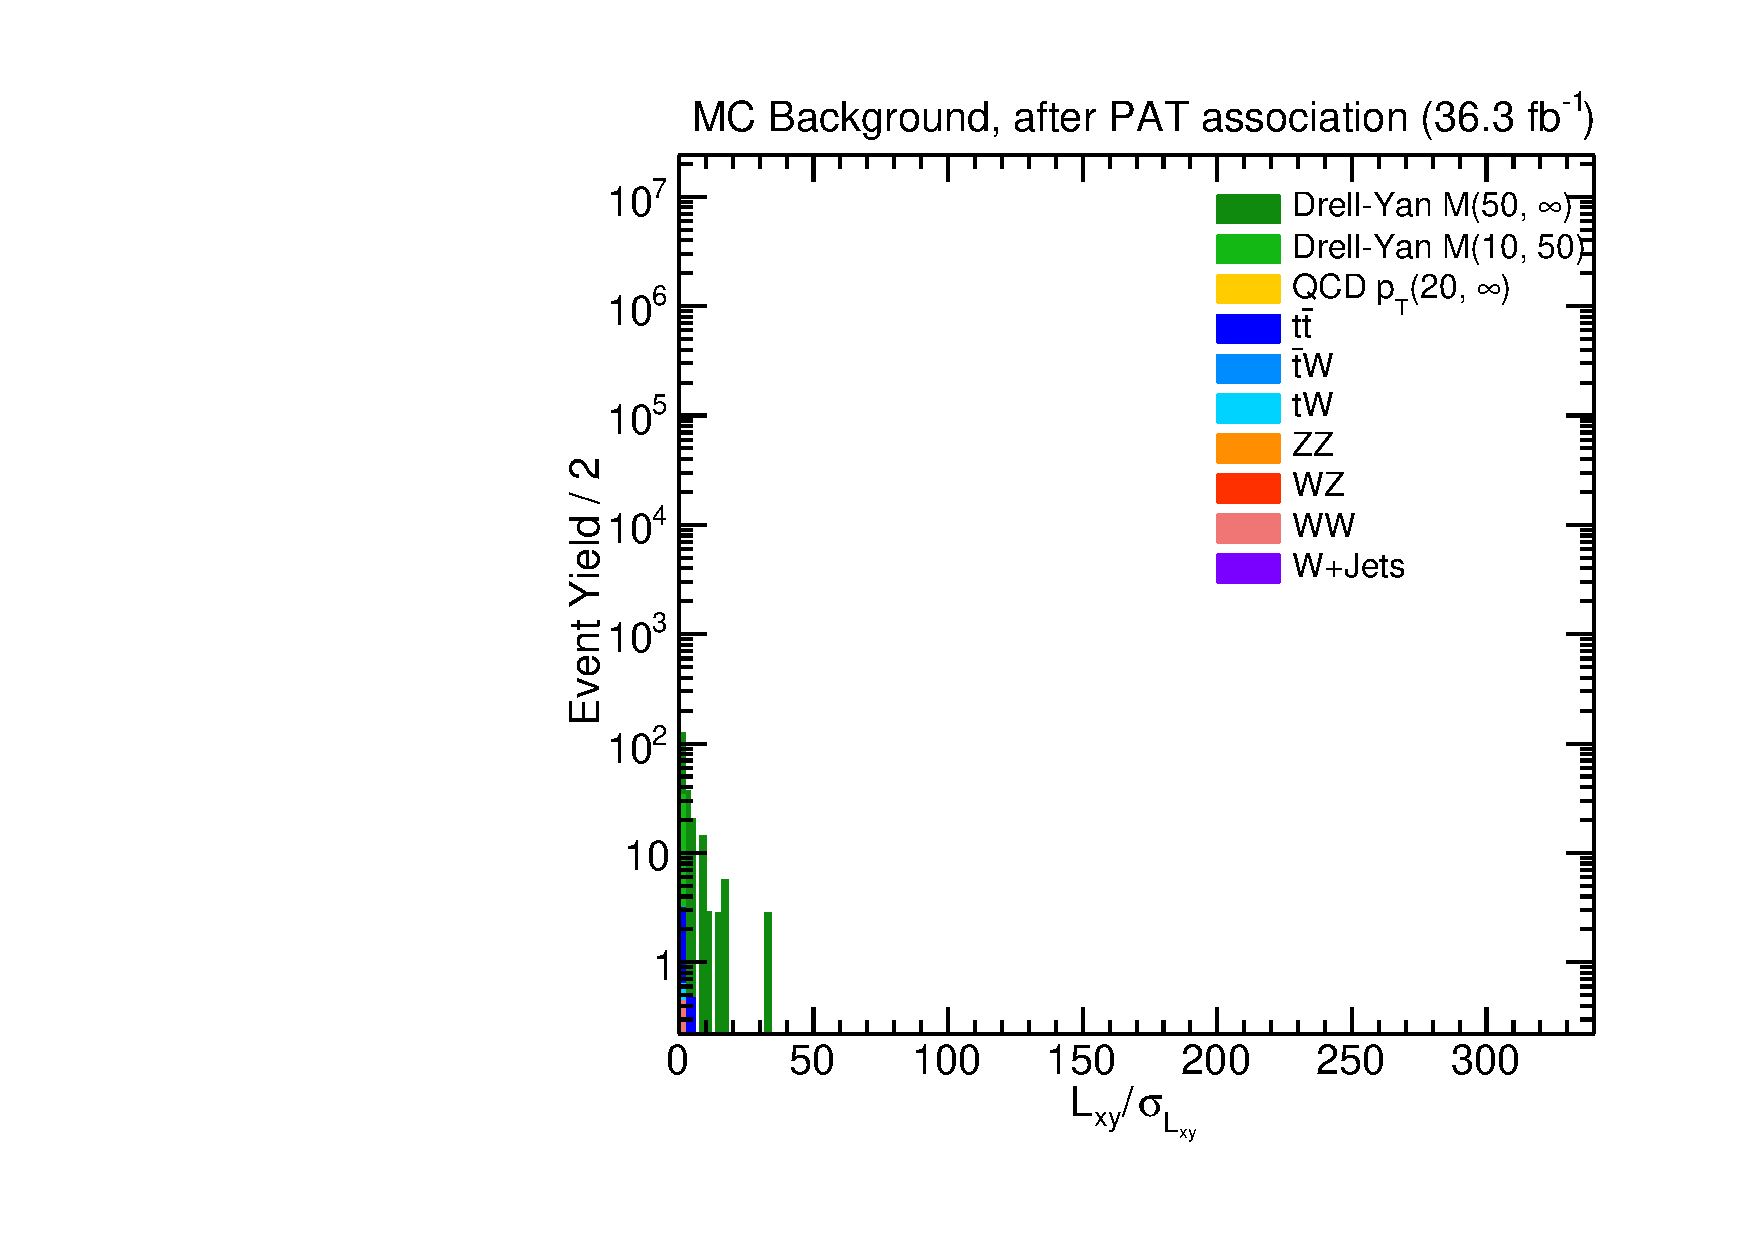
\includegraphics[width=\DSquareWidth]{figures/displaced/REPEFF_MC_LxySig-after.pdf}
  \caption[Histogram of dimuon \LxySig in simulated background samples before and after the PAT association procedure.]{Histogram of dimuon \LxySig in simulated background samples, scaled to 2016 integrated luminosity, \figpos{left} before and \figpos{right} after the PAT association procedure. The procedure suppresses the number of background events by a factor of $10^5$.}
  \label{fig:dd:REPEFF_MC_LxySig}
\end{figure}
\begin{figure}[p]
  \centering
  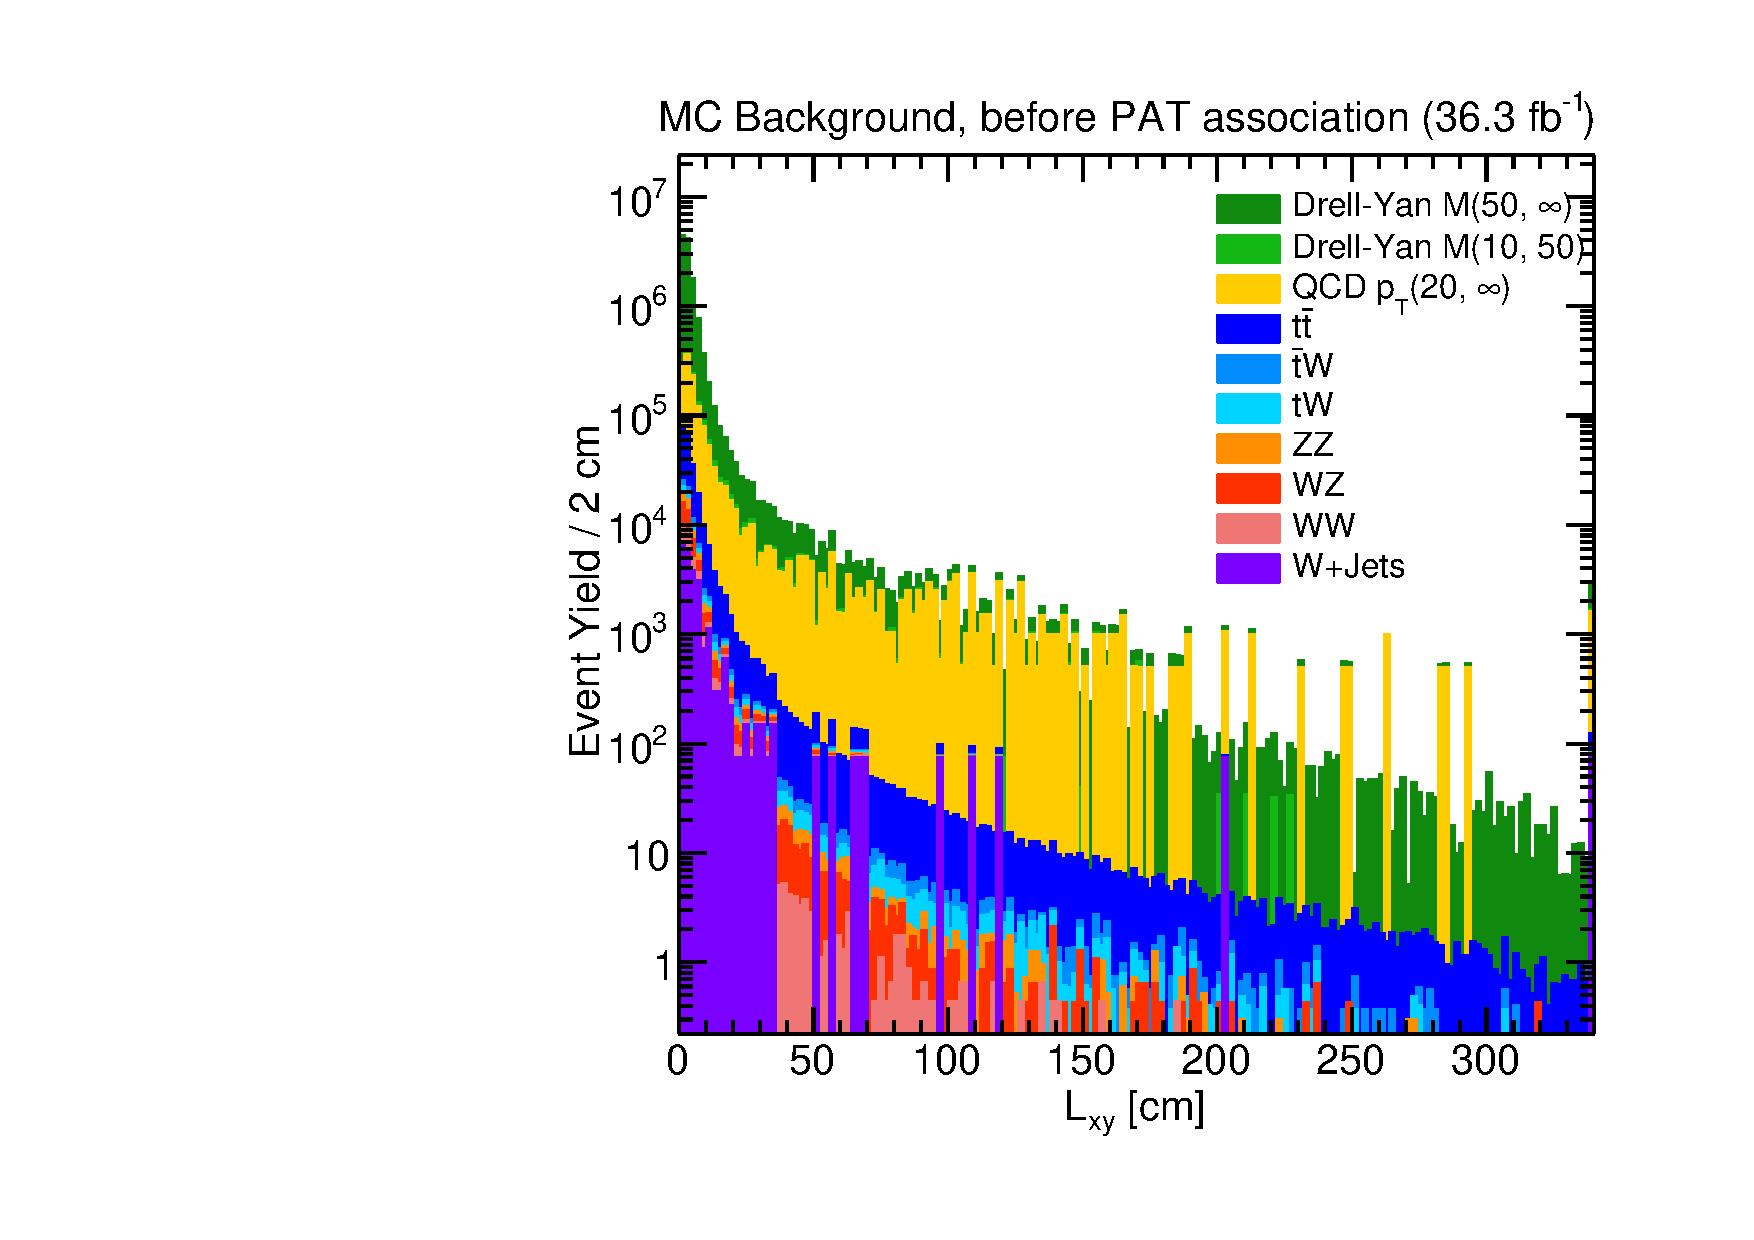
\includegraphics[width=\DSquareWidth]{figures/displaced/REPEFF_MC_Lxy-before.pdf}
  \hspace*{-2em}
  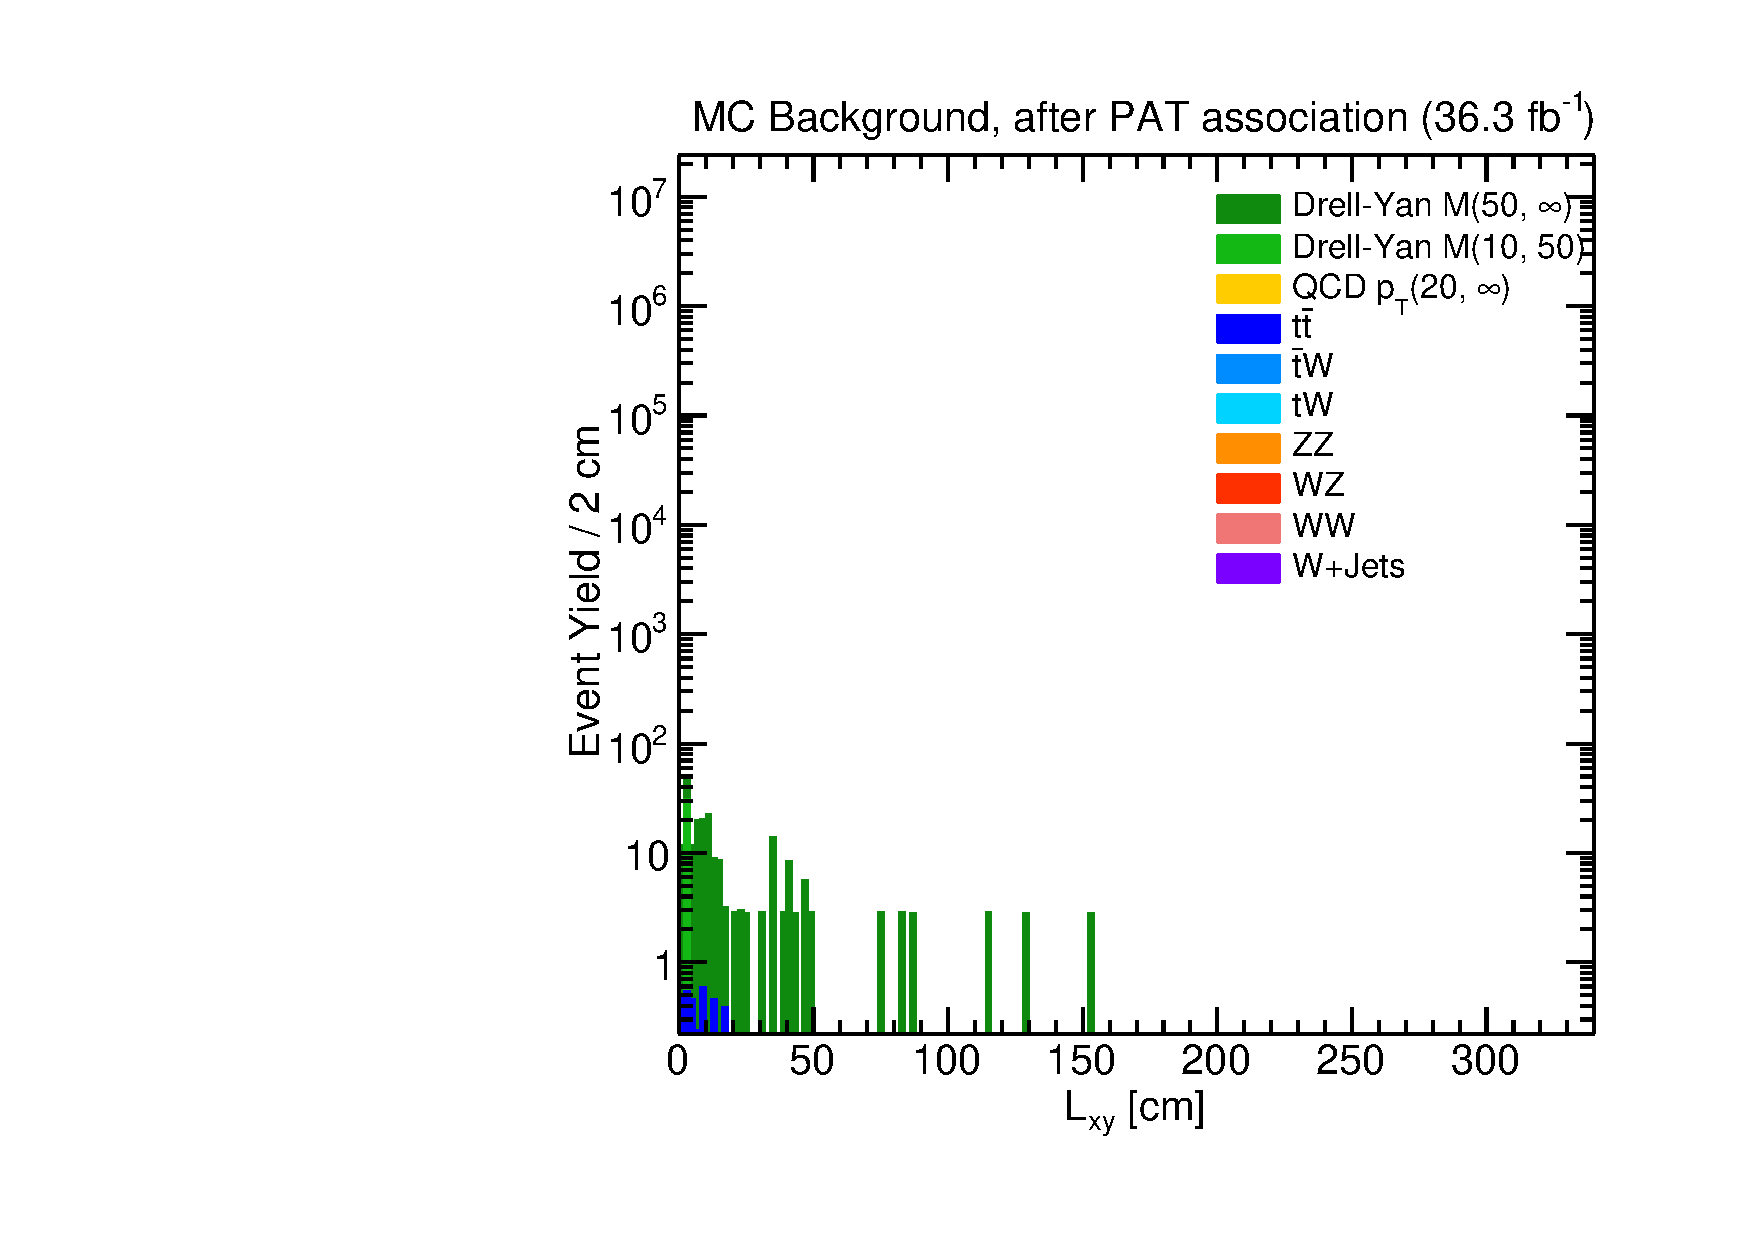
\includegraphics[width=\DSquareWidth]{figures/displaced/REPEFF_MC_Lxy-after.pdf}
  \caption[Histogram of dimuon \Lxy in simulated background samples before and after the PAT association procedure.]{Histogram of dimuon \Lxy in simulated background samples, scaled to 2016 integrated luminosity, \figpos{left} before and \figpos{right} after the PAT association procedure. The procedure suppresses the number of background events by a factor of $10^5$.}
  \label{fig:dd:REPEFF_MC_Lxy}
\end{figure}

In contrast, the association procedure essentially leaves true signal events with dimuon decays outside the tracker relatively untouched.
\Fig~\ref{fig:dd:REPEFF_Signal_Lxy} is a graph of the number of dimuons (matched to generated signal muons by choosing the closest DSA muons to each generated muon in a cone of $\deltaR < 0.2$ between their momentum directions) remaining after PAT association (\ie composed of DSA muons not associated with PAT muons), divided by the number of dimuons before PAT association, as a function of generated \Lxy.
In order to have a sufficient sample size, all 33 of the \twoMu signal samples are combined together for these graphs.
The association efficiently rejects signal events with decays inside the tracker volume, $\Lxy < 65\cm$, while rejecting no more than 10\% of signal events with decays outside the tracker volume, $\Lxy > 65\cm$.
\begin{figure}[htpb]
  \centering
  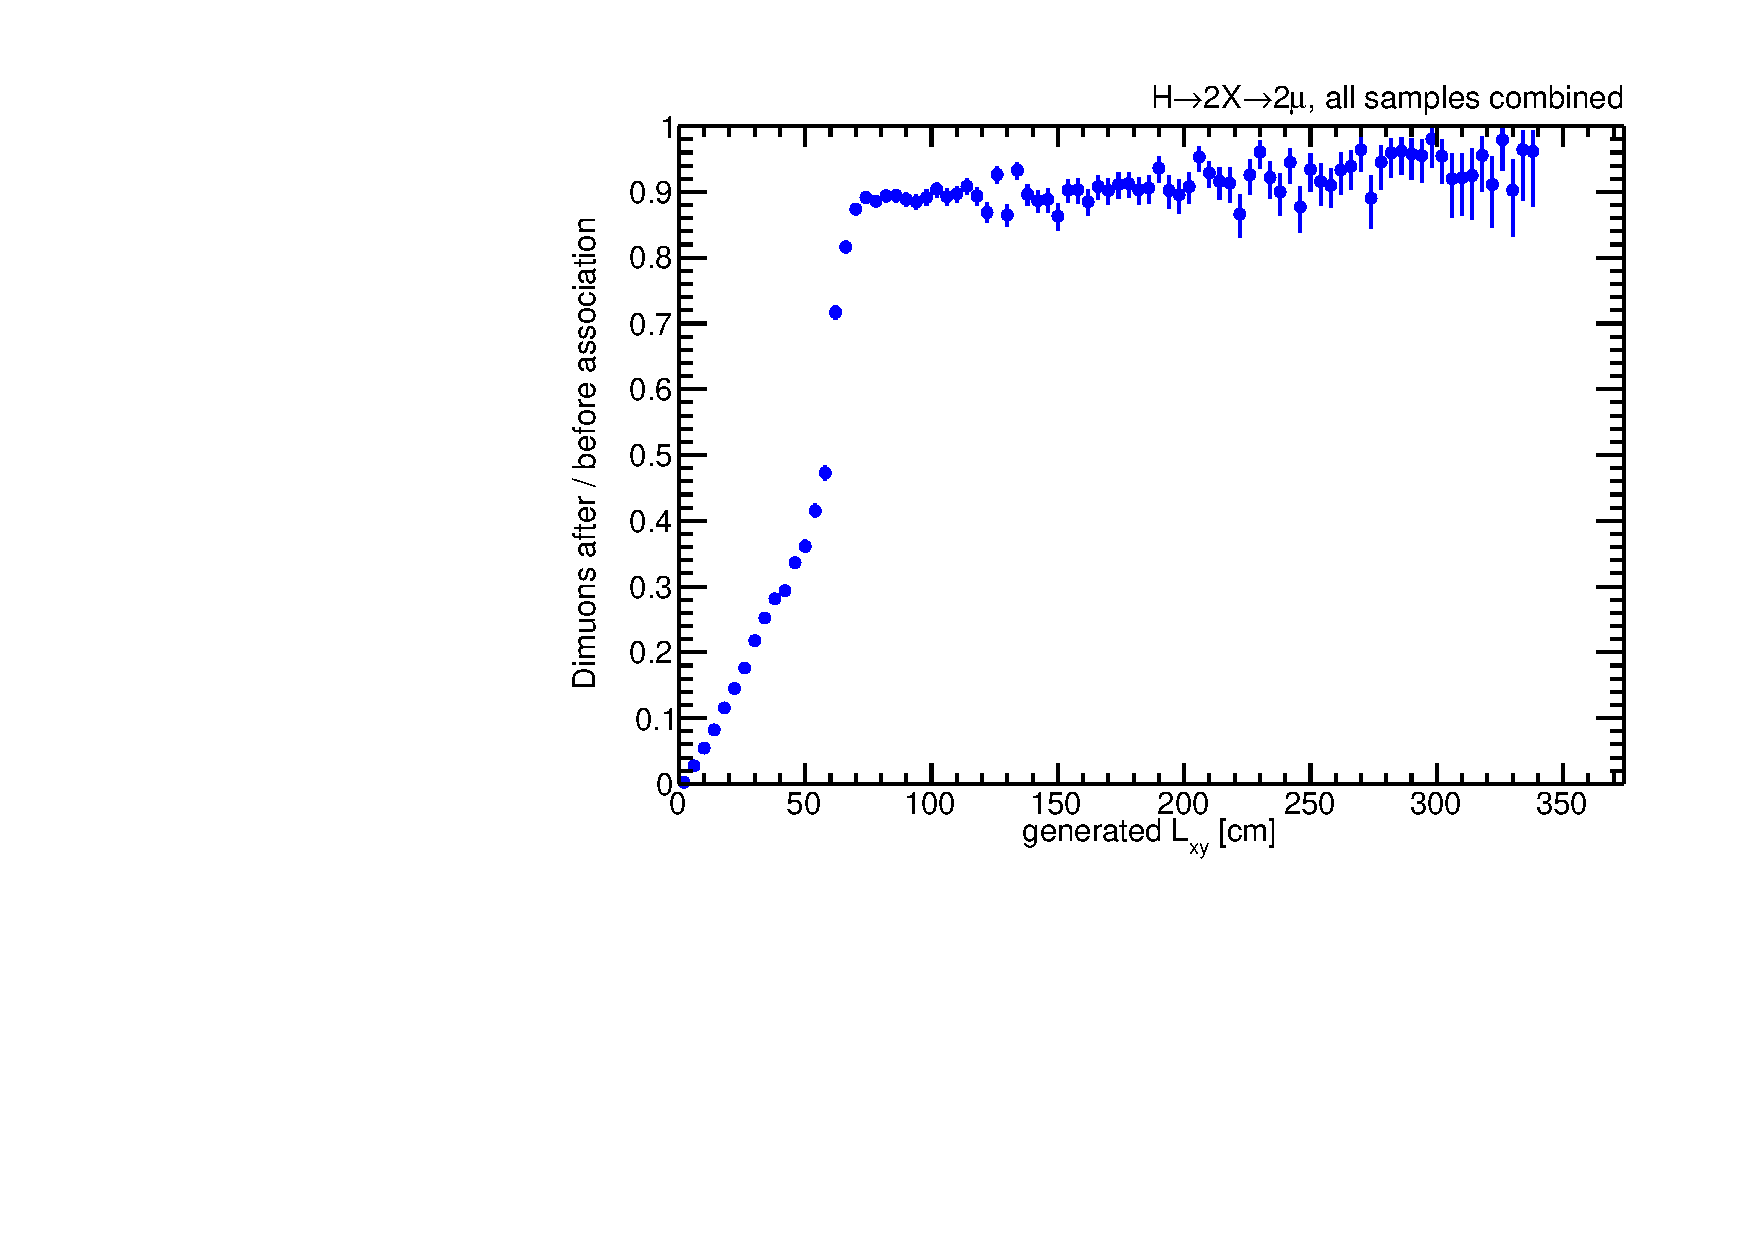
\includegraphics[width=\DFigWidth]{figures/displaced/REPEFF_Signal_Global.pdf}
  \caption[Graph of the number of dimuons after the PAT association divided by the number of dimuons before the PAT association, as a function of generated \Lxy, in all \twoMu signal samples combined.]{Graph of the number of dimuons after the PAT association divided by the number of dimuons before the PAT association, as a function of generated \Lxy, in all \twoMu signal samples combined. This graph shows that the association performs as expected, primarily rejecting signal events whose decays occurred within the tracker volume, while accidentally replacing no more than 10\% of events outside the tracker volume.}
  \label{fig:dd:REPEFF_Signal_Lxy}
\end{figure}


\subsection{DSA Muon Object Selection}
\label{sec:dd:DSAObject}
After the \DSAToPAT association step explained in the previous section, the analysis considers DSA muons not associated with any PAT muons.
As DSA muons are not used by many CMS analyses, a standard set of selections to identify DSA muons does not exist.
In order to further select high-quality DSA muons as well as to discriminate signal-like events from background-like events, the following requirements, along with the DSA muon preselection cuts explained in \Sec~\ref{sec:dd:DSAQuality}, serve as the DSA muon identification selection.
DSA muons are required to have
\begin{itemize}
  \item muon $\pT$ of at least 10\GeV, \ie $$\pT > 10\GeV$$
  \item \normchisq of the muon track fit of at most 2.5, \ie $$\chisq_\text{track}/\text{dof} < 2.5$$
  \item at least 19 hits in the DTs for muons reconstructed only in the barrel, \ie $$N(\text{CSC hits}) = 0 \implies N(\text{DT hits}) > 18$$
  \item time with respect to bunch crossing of at most 12\unit{ns}, \ie $$|t_\text{in-out}| < 12\unit{ns}$$
\end{itemize}

The \pT cut suppresses background events, which often have poor quality muons with low \pT, including background events arising from QCD processes.
The track \normchisq cut ensures that the muons are reasonably well reconstructed.
The $N(\text{DT hits})$ cut discriminates signal events from background events.
The timing cut is explained in \Sec~\ref{sec:dd:timing}.

\pagebreak
\subsubsection{In-Time with Triggering Bunch Crossing Requirement}
\label{sec:dd:timing}
A potentially pernicious class of events that can mimic displaced dimuon decays arises from a combination of technical features in the trigger and readout electronics of the muon chambers and the silicon tracker.
In a normal event with two muons, the timing of the trigger pulse from the two muons in the muon chambers is correctly aligned in time with the hit readout of the muon chambers and the tracker.
It can happen, however, that jitter in the muon trigger electronics creates a \Lone trigger signal that is 25\unit{ns} earlier than normal.
In the muon system readout, the muon hits are still recorded, but they have hit times that are 25\unit{ns} later than normal (since they are measured with respect to the \Lone trigger signal that is 25\unit{ns} too early).
When there is an early \Lone trigger signal, in contrast, the tracker hits associated with the triggering muons are \emph{not} recorded; tracker hits from unrelated \pp collisions 25\unit{ns} earlier are recorded instead.
The offline reconstruction code then finds the two triggering muons, but not the associated tracker tracks.
This mimics the main feature of displaced muons: tracks in the muon system with no associated tracker tracks.

Fortunately, the recorded times of the hits in the muon system provide a means to recognize such (very rare) events.
In practice, the time of the DSA muons is obtained from a precision timing algorithm that is implemented for standard standalone (SA) muons.
This algorithm provides a time that is centered on zero for normal muons, with jitter of a few nanoseconds, computed by extrapolating to the interaction point the times each constituent hit was formed with respect to the bunch crossing, under the hypothesis that the muon was produced in the detector and traveled outwards.
This time is referred to as $t_\text{in-out}$.

Matching DSA muons to SA muons is straightforward: DSA muons with an SA muon within a \deltaR cone of 0.2 are considered matched to the SA muon.
The time associated with the SA muon can be used to distinguish between normal muons and the pathological cases where the times are centered on non-zero multiples of 25\unit{ns} (the time between bunch crossings).
This requirement is implemented as the requirement $|t_\text{in-out}| < 12\unit{ns}$, and is more than 99\% efficient for simulated samples of the \twoMu signal.

\pagebreak
This class of background was understood only after unblinding the signal region, and so this selection criterion was added with the knowledge that it would eliminate some events.
However, we believe that this is a clear case that any bias due to adding this criterion is negligible, and that it would be foolish not to add this criterion, given our current understanding of this background.

\subsection{Dimuon Formation from Common Vertex Fit}
\label{sec:dd:DimVertex}
A decay of a long-lived particle to two muons is detected as a pair of muons originating from a common vertex, so at this stage, pairs of reconstructed muons are investigated together for consistency with originating from a common vertex and from the decay of a massive, long-lived particle.
A pair of DSA muon tracks fit to a common vertex, along with the four-momentum sum of the two muons, is referred to as a dimuon.
All $n(n-1)/2$ possible pairs of distinct DSA muons among $n$ selected DSA muons are initially considered when forming dimuons.
This set of pairs is immediately filtered by requiring that the distance of closest approach (DCA) of the two DSA tracks helically extrapolated in the magnetic field is less than 50\unit{cm}:
$$\text{DCA} < 50\unit{cm}$$
This is a loose requirement ensuring that the common vertex fit is not performed on a pair of tracks that never come close to approaching each other.

\subsubsection{Vertex Fitting}
\label{sec:dd:VertexFitting}
The common vertex fit is performed by an implementation of the Kalman filter algorithm in the CMS software, called the \Code{KalmanVertexFitter} \cite{Fruhwirth:1987fm,Speer:927395}.
The default implementation in the CMS software version used in this analysis restricts the range of the location of the fitted vertex to approximately within the boundary of the silicon tracker.
In this analysis, this restricted range is extended to the beginning of the muon system in order to efficiently reconstruct a common vertex for particles decaying outside the tracker.

The technical changes to the CMS software are documented here.
The following changes were made to \Code{RecoVertex/VertexTools/src/SequentialVertexFitter.cc}:
\begin{itemize}
  \item \Code{TrackerBoundsRadius} was changed from 112 to 500
  \item \Code{TrackerBoundsHalfLength} was changed from 273.5 to 1000
\end{itemize}

The results of the common vertex fit are used to define dimuon quantities such as transverse decay length.
As the existence of a common vertex fit is necessary to further study dimuon properties and consistency, the common vertex fit is required to converge.
The common vertex fit modifies the input tracks in order to be consistent with originating from a common vertex; these tracks are referred to as ``vertex-constrained'', and any of the muon properties (\pT, direction, \etc) may be different in the vertex-constrained version of the track than in the original version.
For many purposes, the vertex-constrained tracks are preferable because they represent a reconstruction performed with more information.
However, in a few situations, the vertex fitter fails or produces nonsensical results.
A few of the features of the fitter are documented here.

\begin{figure}[htpb]
  \centering
  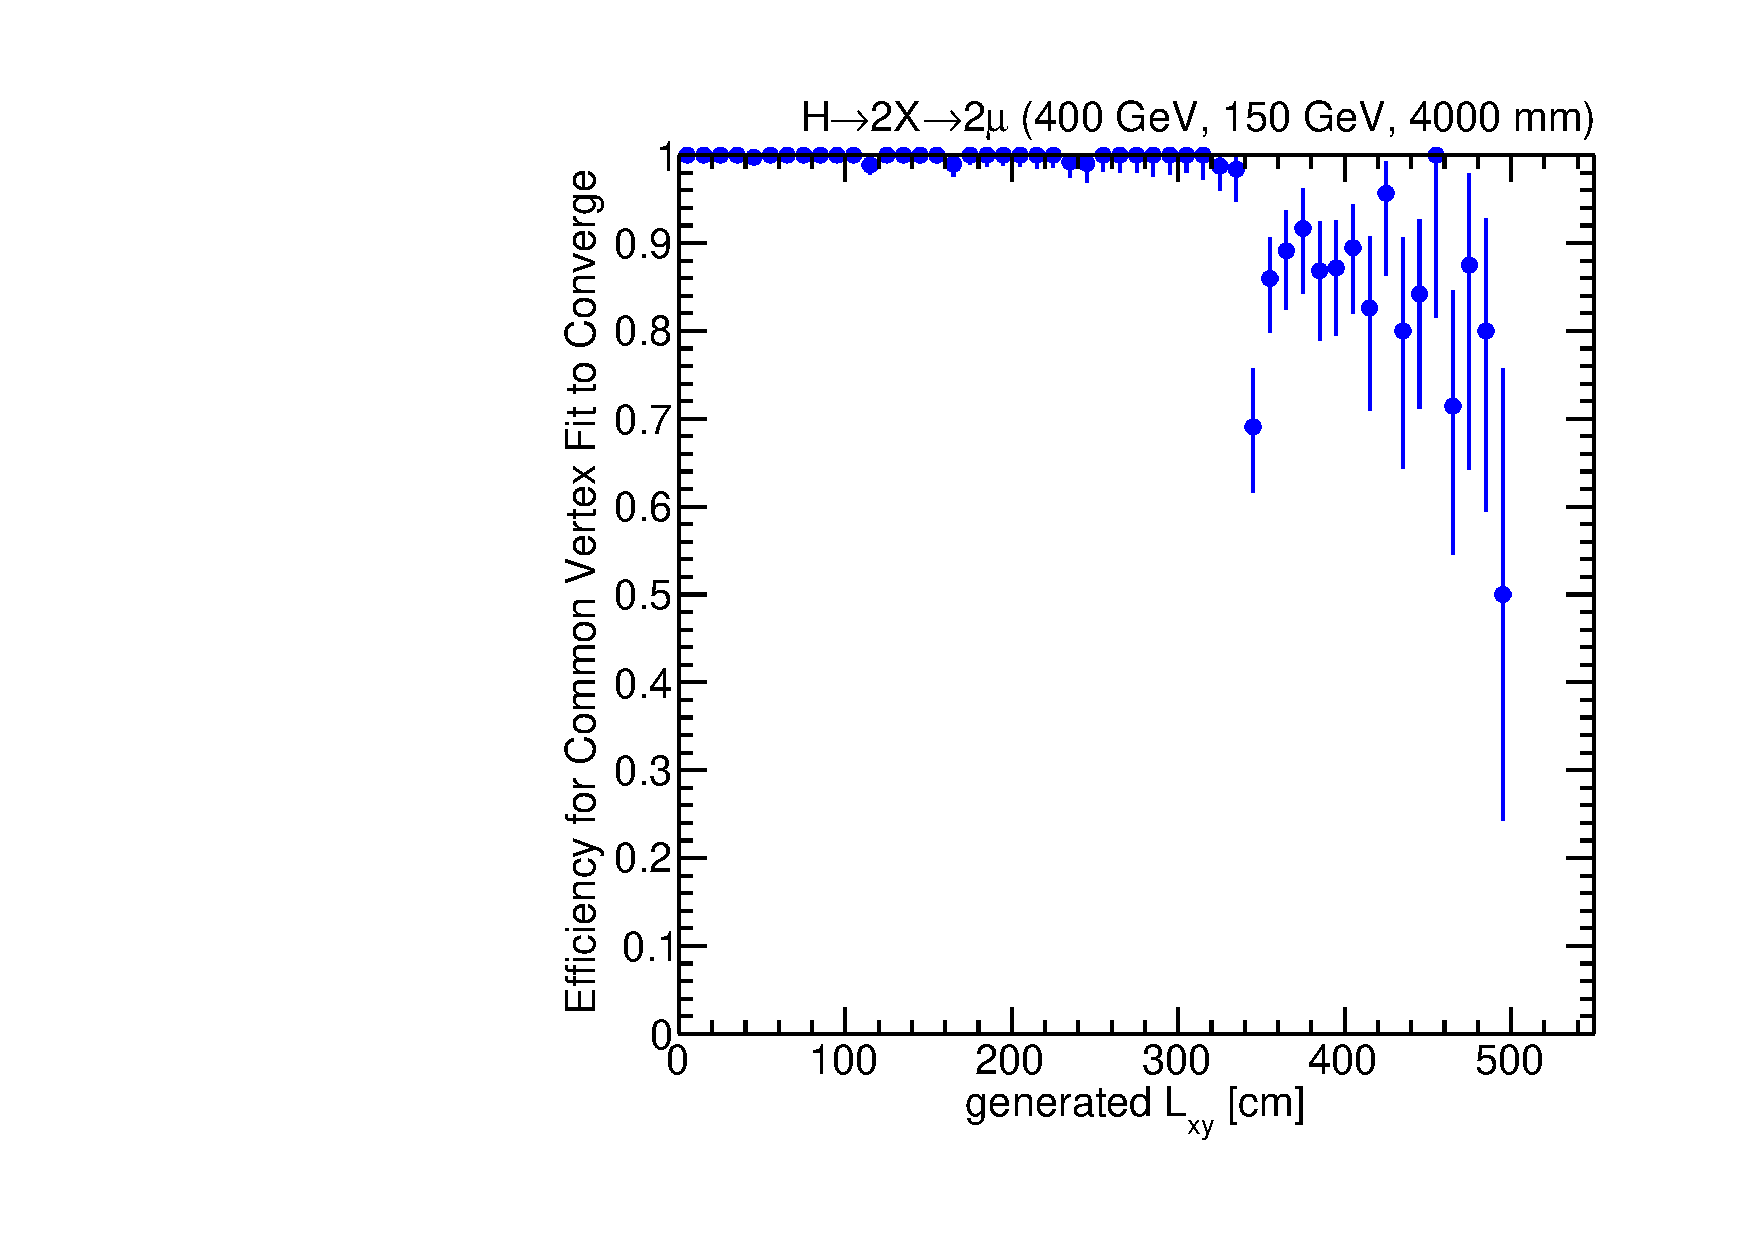
\includegraphics[width=\DSquareWidth]{figures/displaced/VFE_Lxy_2Mu2J_400_150_4000.pdf}
  \hspace*{-2em}
  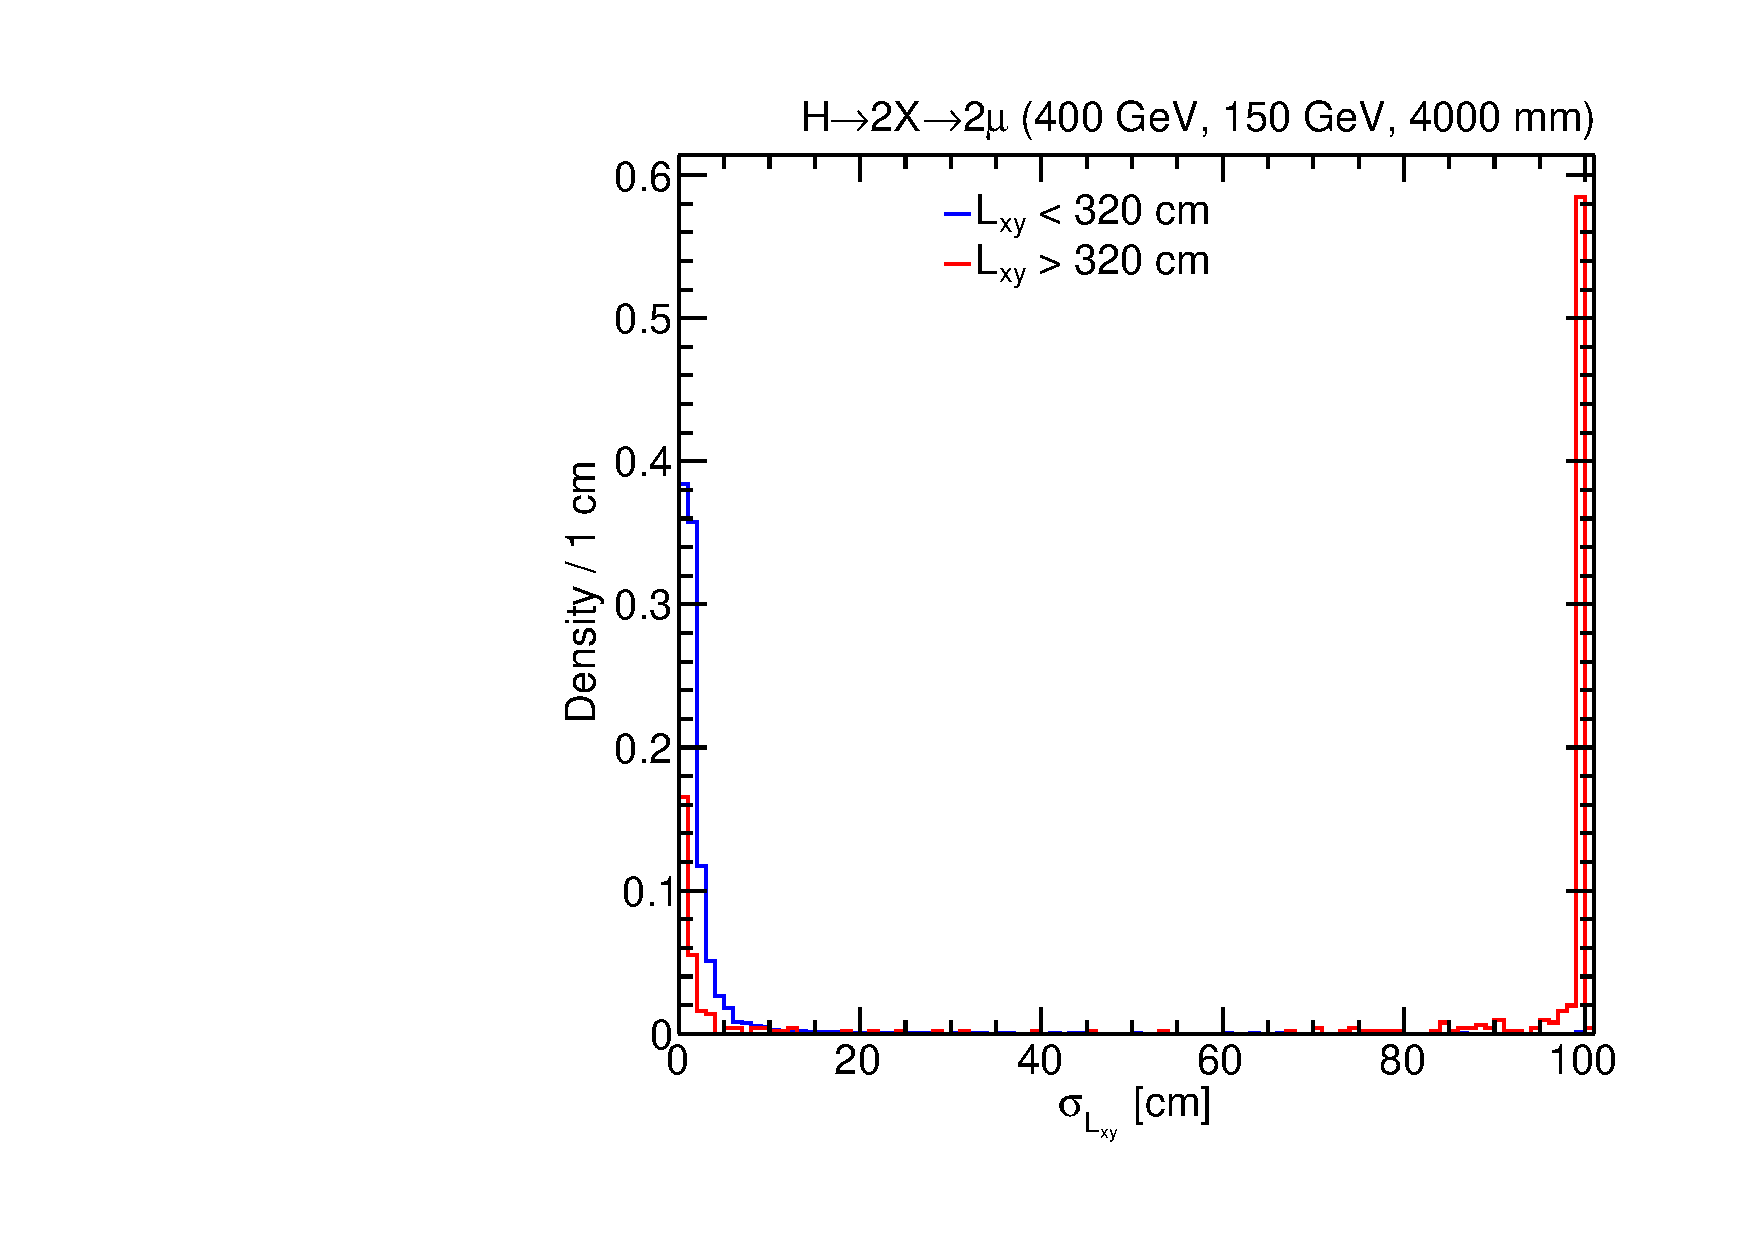
\includegraphics[width=\DSquareWidth]{figures/displaced/LESSMORE_LxyErr_2Mu2J_400_150_4000.pdf}
  \caption[Efficiency for the common vertex fit to converge as a function of generated \Lxy for generated events within acceptance and histograms of \LxyErr normalized to unit area for $\Lxy < 320\cm$ and $\Lxy > 320\cm$.]{\figpos{Left} Efficiency for the common vertex fit to converge for the \twoMu signal sample with \FullSP{400}{150}{4000} as a function of generated \Lxy, for generated events within acceptance. Both the preselection and object selection cuts are applied to DSA muons. In this graph, events are not required to pass the trigger, the HLT-RECO matching requirement was dropped, and the \DSAToPAT association procedure was not performed. Error bars are for the statistical uncertainty only. \figpos{Right} Histograms of \LxyErr normalized to unit area for the events in the numerator of the left plot, separately for $\Lxy < 320\cm$ and $\Lxy > 320\cm$, for the \twoMu signal sample with \FullSP{400}{150}{4000}, for generated events within acceptance. The distribution for $\Lxy > 320\cm$ has a large peak near 100\cm.}
  \label{fig:dd:VertexFitAnomalies}
\end{figure}

The vertex fit does not always converge for an arbitrary pair of tracks.
The left plot of \Fig~\ref{fig:dd:VertexFitAnomalies} is a graph of the efficiency for the common vertex fit to converge, with respect to signal events in which both generated muons are reconstructed as DSA muons, as a function of the generated \Lxy, for the \twoMu signal sample with \FullSP{400}{150}{4000}.

The denominator of this efficiency is the number of generated events within acceptance (both generated muon $\pT > 25\GeV$, both generated muon $|\eta| < 2$, and generated \mbox{$\Lxy < 500\cm$}) in which both generated muons had matching DSA muons.
That is, each generated muon has a DSA muon passing the muon preselection and the muon object selection within a cone of $\deltaR < 0.2$ between their momentum directions.
The numerator of this efficiency is the number of such events in which the dimuon common vertex fit converged for the two matched muons.
In order to observe the effect of the common vertex fit independently of the low trigger efficiency at large \Lxy, events are not required to pass the trigger and the HLT-RECO matching requirement was dropped.
In order to have a sufficient sample size, the \DSAToPAT association procedure was not performed.

Convergence of the vertex fit is highly efficient when fitting two DSA muon tracks that are matched to generated signal muons produced from long-lived particle decaying in the detector up to transverse displacements of 330\unit{cm}.
Beyond 330\unit{cm}, the efficiency for the common vertex fit to converge drops dramatically.

For those events beyond 330\unit{cm} that do converge, the fit quality is often quite poor, \eg the \pT resolutions of the vertex-constrained tracks are worse than before the fit.
Finally, many of these events retain an internal \Lxy uncertainty (\LxyErr) of a default value of 100\cm.
The right plot of \Fig~\ref{fig:dd:VertexFitAnomalies} shows distributions, normalized to unit area, of the events in the numerator of the left plot of \Fig~\ref{fig:dd:VertexFitAnomalies}, separately for $\Lxy < 320\cm$ and $\Lxy > 320\cm$.
A large fraction of the events with $\Lxy > 320\cm$ have \LxyErr near 100\cm.
Such events would have a small \Lxy significance (3 or less) and would not pass an analysis selection.
This type of common vertex fit failure would result in the loss of these events, even though the fit converged.

As in the Run~1 analyses, the trigger efficiency at such large \Lxy values is quite small, and the \LxySig selection discussed in \Sec~\ref{sec:dd:DimuonSignal} usually suppresses such events as well.
Therefore, further study of these events and attempts to rescue them from the behavior of the vertex fitter are of low priority for this analysis, and the underlying causes for this behavior remain a curiosity.

\subsection{Pairing Criteria}
\label{sec:dd:PC}
Considering all possible pairs of DSA muons results in many dimuons formed from DSA muons that are not related in any way.
It is therefore important to develop criteria that choose the correct reconstructed dimuons with high efficiency, consistent with signal.
Selections on individual dimuons (such as requiring the \vchisq to be small) impose some quality constraints that are useful for selecting such dimuons, but any set of criteria that determines which pairs of muons form the correct dimuons must consider the event as a whole.
Choosing such a set of pairing criteria is particularly subtle in, for example, decays of two long-lived particles into a final state with 4 muons.
The 4 muons can be nominally paired into 6 overlapping dimuons, which can be partitioned into three distinct sets of 2 dimuons with no shared muons; the criteria must choose between them.
This situation is made more complex when, among other things,
\begin{itemize}
  \setlength\itemsep{.2\baselineskip}
  \item one or more muons are not reconstructed
  \item duplicate muons are reconstructed from partial sets of hits
  \item muons are not all reconstructed with the correct charge
  \item pairs of muons are highly collimated and distinguishing them is difficult
  \item vertex fits of muons from different long-lived particle decays yield a good \vchisq
\end{itemize}
In developing this set of pairing criteria, several combinations of metrics were considered.
\begin{itemize}
  \setlength\itemsep{.2\baselineskip}
  \item Dimuon(s) formed from the highest \pT muons in the event
  \item Dimuon(s) with the least \vchisq in the event
  \item Dimuon(s) formed from muons with charges of opposite sign
  \item Pairs of dimuons with the least sum of \vchisq
  \item Pairs of dimuons with the least difference in reconstructed dimuon mass
\end{itemize}
\Fig~\ref{fig:dd:pc} is a diagram illustrating the application of the pairing criteria to the set of all possible dimuons in the case of four selected muons.
\begin{figure}[htpb]
  \centering
  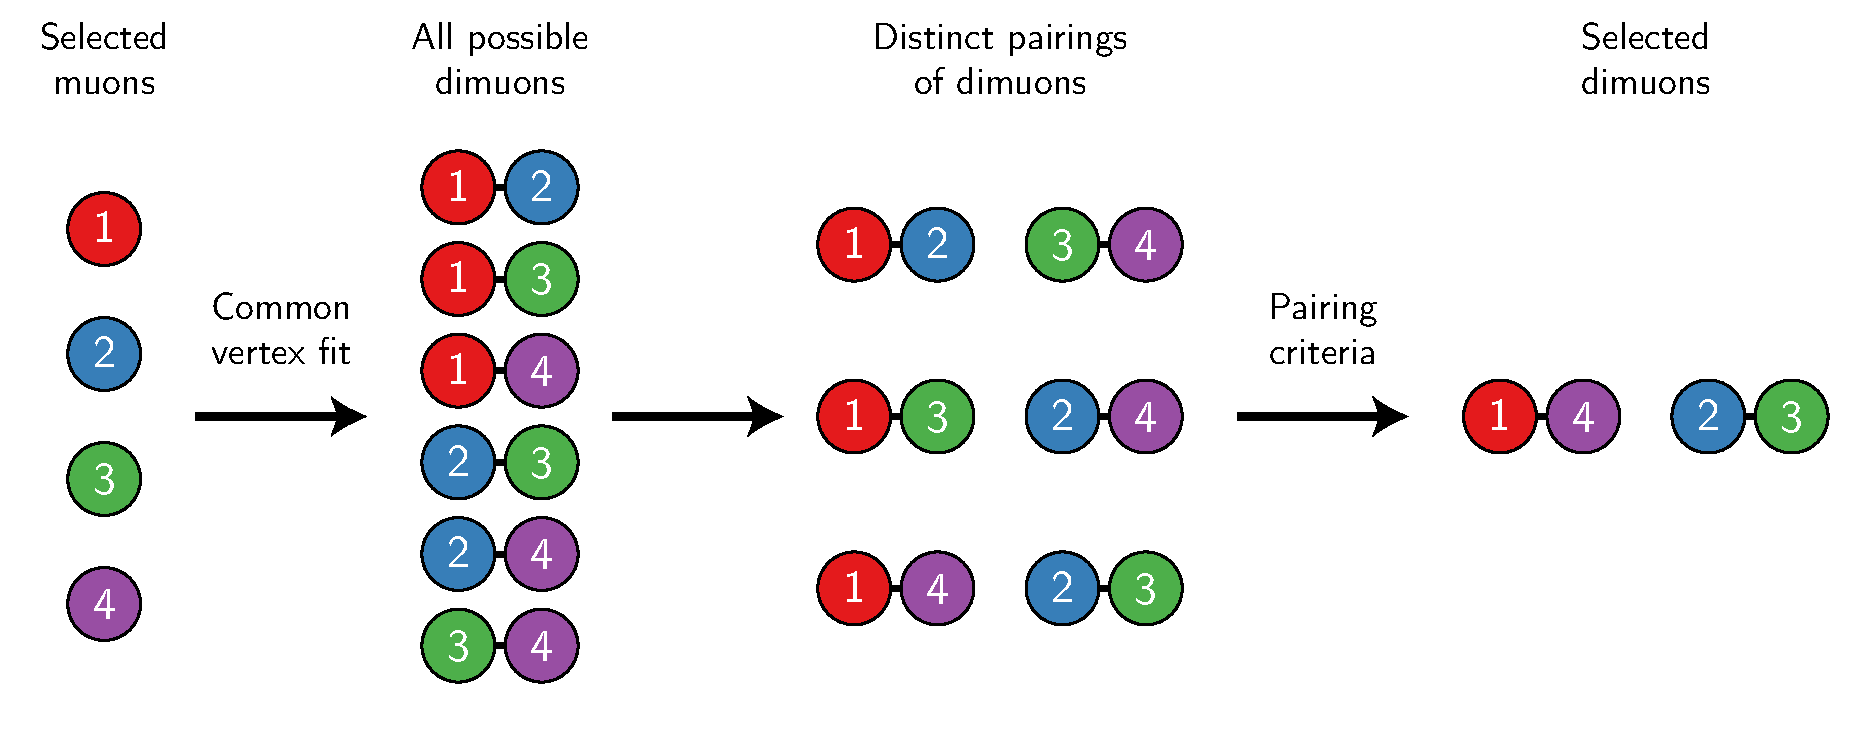
\includegraphics[width=\textwidth]{figures/displaced/PairingCriteriaDiagram.pdf}
  \caption[Diagram illustrating the application of pairing criteria to dimuons in the case of four selected muons.]{Diagram illustrating the application of pairing criteria to dimuons in the case of four selected muons. Four muons may be paired into six dimuons whose constituent muons overlap. These six dimuons may be partitioned into three distinct pairings of dimuons, in which no muons are shared between dimuons. Pairing criteria select the correct pair of dimuons consistent with a four muon signal event.}
  \label{fig:dd:pc}
\end{figure}

Potential pairing criteria were studied and optimized on both the \twoMu and \fourMu simulated signal samples.
Choosing the highest \pT muons in the event is highly correlated with choosing the signal muons, a fact that is robust across all signal sample parameters covering a wide range of long-lived particle lifetimes and muon \pT spectra.
Requiring that dimuons be formed from muons of opposite charge provides only modest efficiency gains with respect to choosing the signal dimuons, and is undesirable at this stage as it introduces dependence on a specific type of signal model.
In events with fewer than four muons, a simple ranking of all possible dimuons by \vchisq yielded the highest efficiency.

The combinatorial space is far richer in events with four or more muons.
For long-lived particles decaying outside the tracker leading to events with at least 4 muons, the criterion yielding the highest efficiency to select signal dimuons is to choose the pair of dimuons whose \vchisq sum is the smallest, among all distinct pairs of dimuons that can be formed from the 4 highest \pT muons in the event. 
An alternative criterion to the least sum of \vchisq is the least difference in reconstructed dimuon mass.
Due to the limited mass resolution of DSA muons, this criterion was found to be less efficient overall than the least sum of \vchisq, except in events with a generated transverse decay length of less than 30\unit{cm}, a region where this DSA muon-based analysis has low sensitivity.
Applying the pairing criteria to an event with any number of dimuons formed from any number of muons results in 2 or fewer selected dimuons for the event.
The full technical details of this procedure are depicted in \Fig~\ref{fig:dd:pca}.

\begin{figure}[htpb]
  \centering
  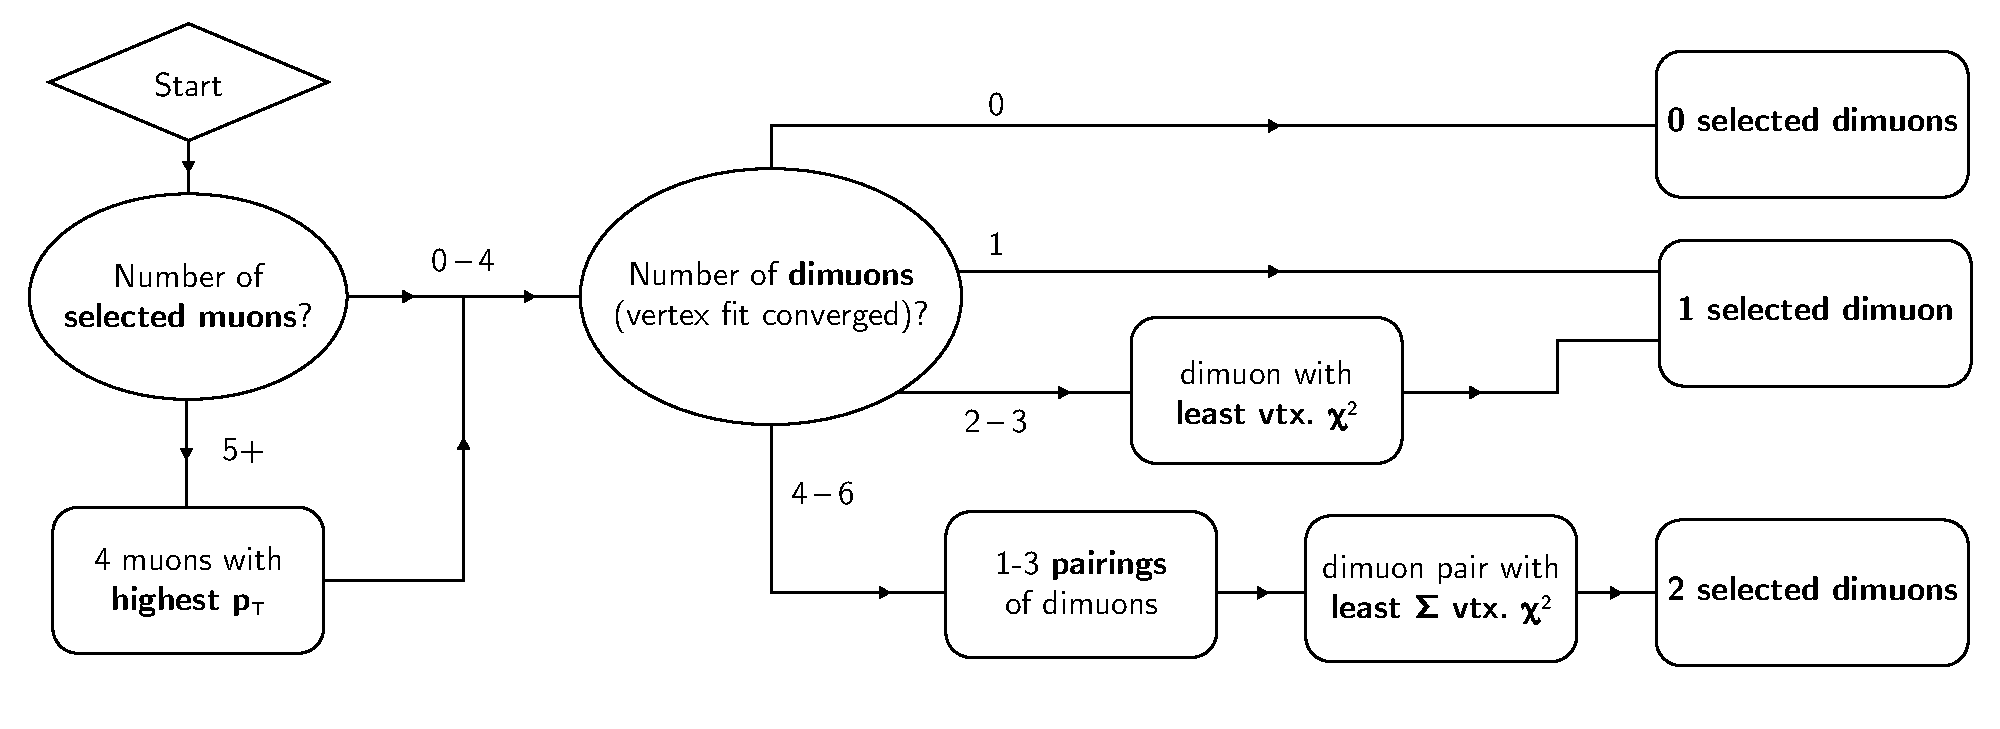
\includegraphics[width=\textwidth]{figures/displaced/PairingCriteriaAlgorithm.pdf}
  \caption[Flowchart depicting the technical details of the pairing criteria procedure.]{Flowchart depicting the technical details of the pairing criteria procedure. Up to 4 DSA muons are selected, ranked by \pT. With the DCA and vertex fit convergence requirements, these muons can be formed into up to 6 dimuons (0 for 0 or 1 muon, up to 1 for 2 muons, up to 3 for 3 muons, and up to 6 for 4 muons). The pairing criteria choose up to 2 dimuons among the possible dimuons.}
  \label{fig:dd:pca}
\end{figure}

\Fig~\ref{fig:dd:PC_Eff} shows graphs of the efficiency for the pairing criteria to correctly select reconstructed dimuons as a function of generated \Lxy, for a selection of \twoMu and \fourMu signal samples.
\Fig~\ref{fig:dd:PC_Eff_Global} shows the same graphs, but for all 33 signal samples combined together.
The denominator of this efficiency is the number of generated signal dimuons matching a reconstructed dimuon (using the closest DSA muons to each generated muon in a cone of $\deltaR < 0.2$ between their momentum directions).
The numerator of this efficiency is the number of reconstructed dimuons chosen by the pairing criteria that are the same as the reconstructed dimuon matched to generated signal.
This efficiency is 97--100\% for \twoMu and 80--98\% for \fourMu signal samples with medium and long lifetimes, for generated transverse decay lengths of $\Lxy > 100 \cm$.
The pairing criteria are less efficient for \fourMu samples with larger values of \mH and smaller values of \mX, because events in such samples consist of two pairs of highly collimated muons, which yield a greater uncertainty in the fitted vertex position in the dimuon momentum direction, and therefore less discriminating vertex \chisq values.

\begin{figure}[p]
  \centering
  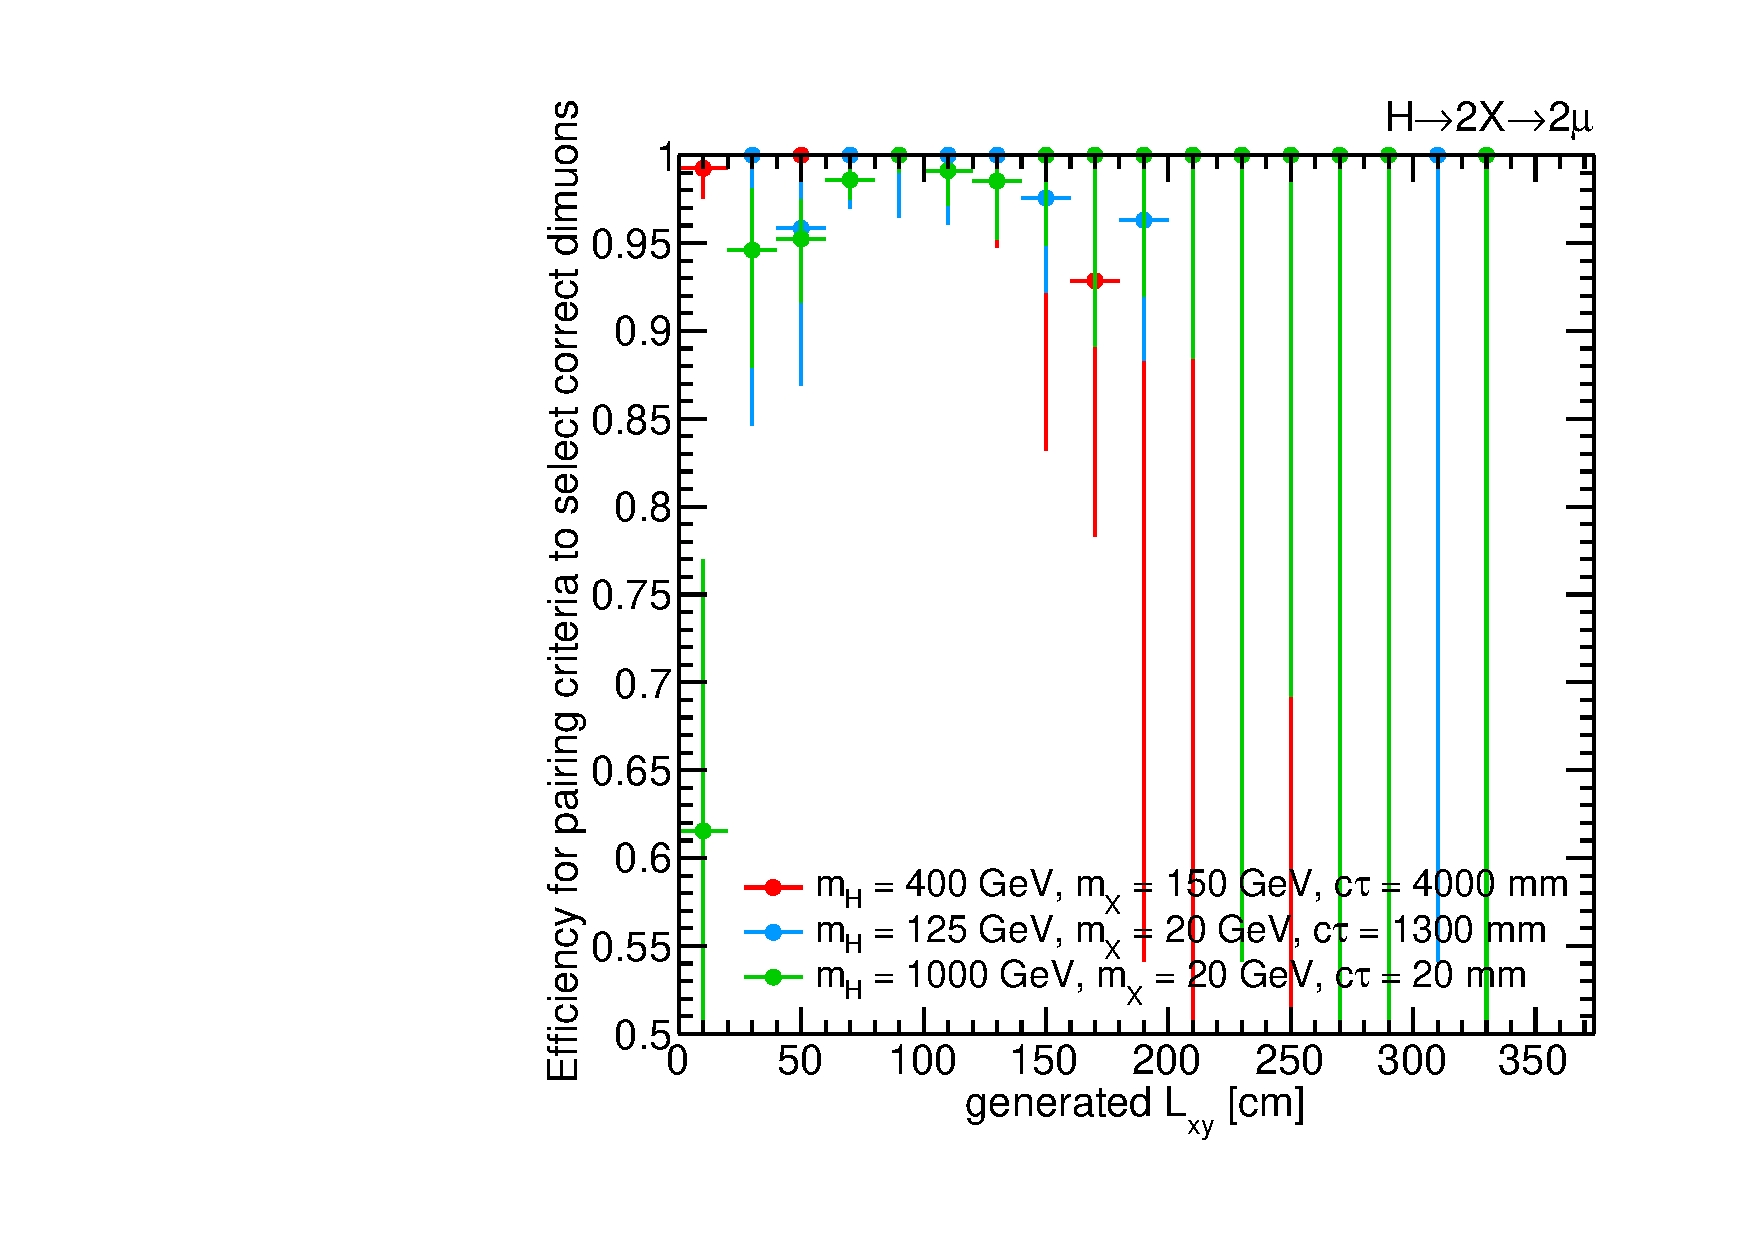
\includegraphics[width=\DSquareWidth]{figures/displaced/PC_Lxy_2Mu2J_Mul.pdf}
  \hspace*{-2em}
  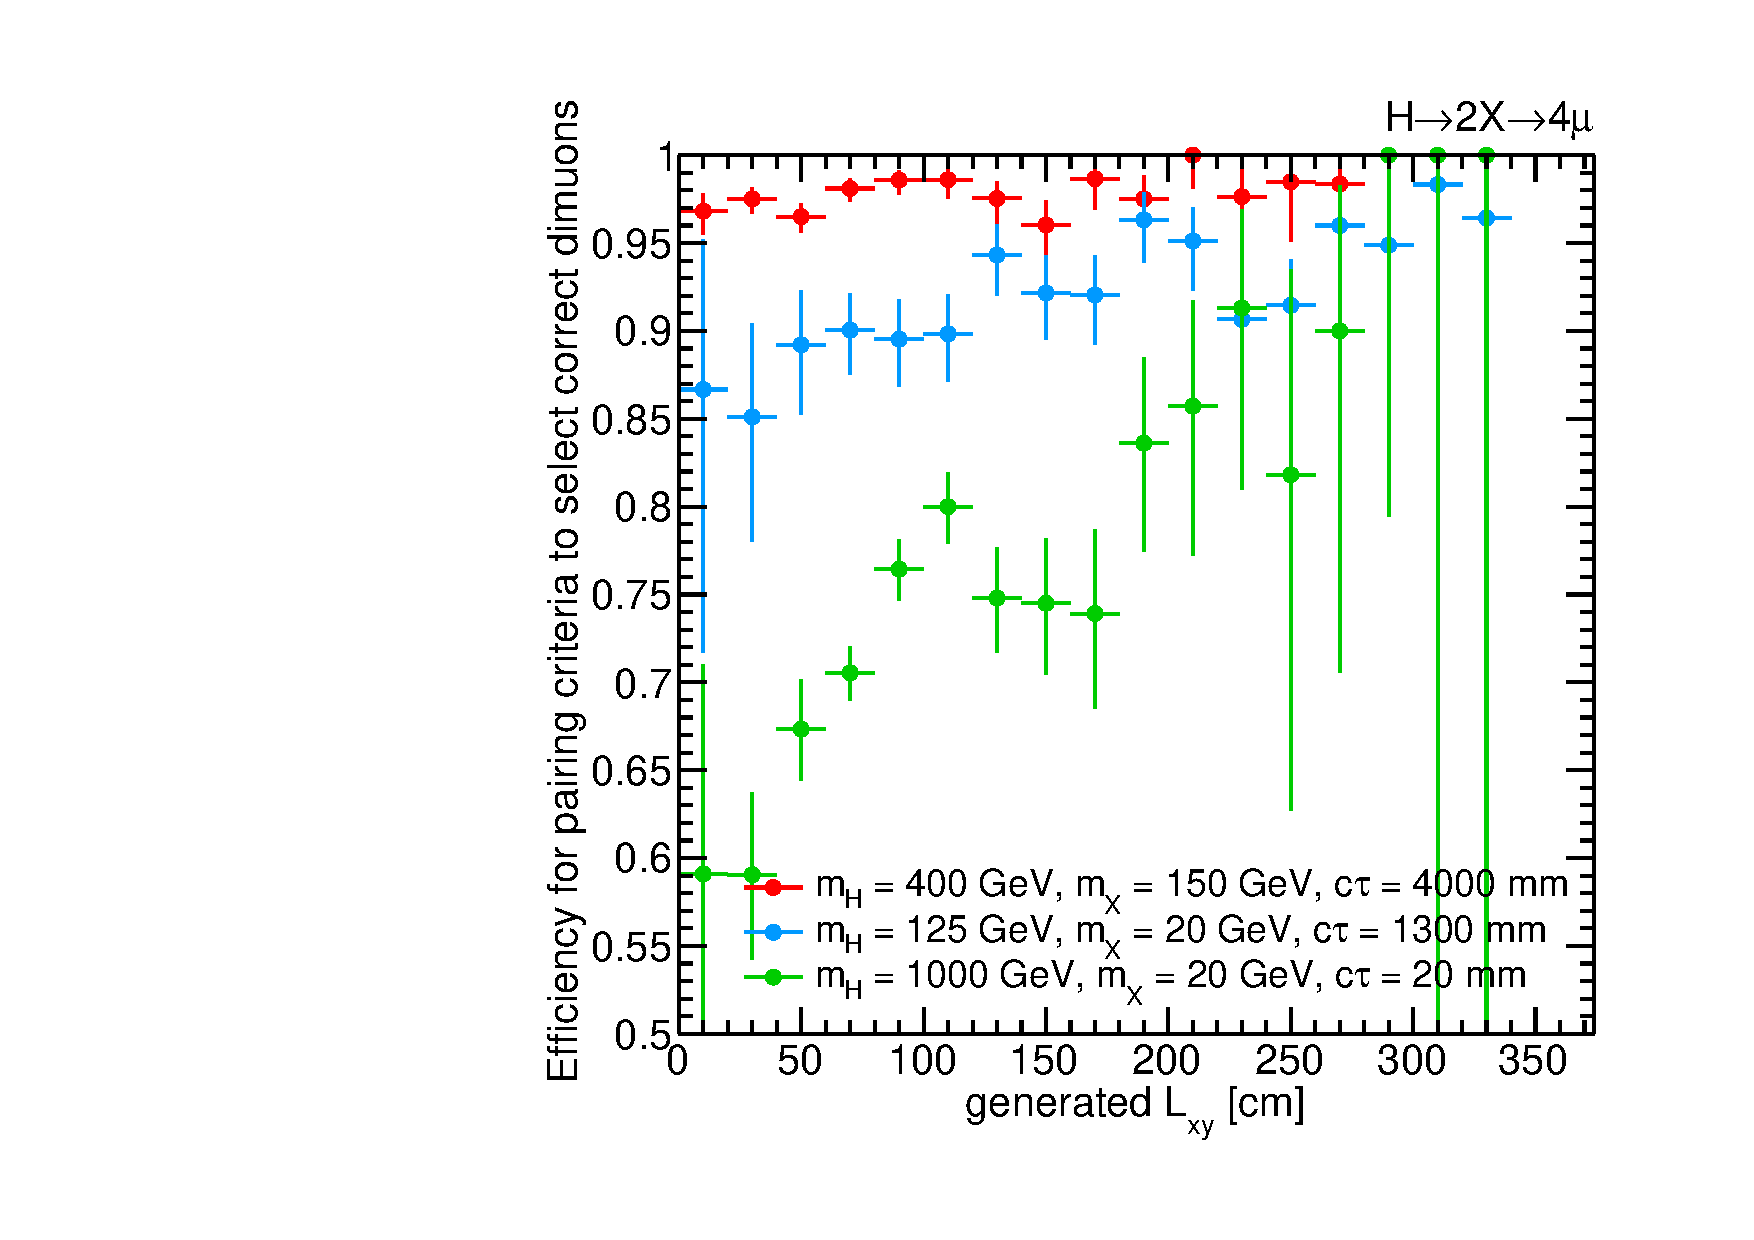
\includegraphics[width=\DSquareWidth]{figures/displaced/PC_Lxy_4Mu_Mul.pdf}
  \caption[Efficiency for the pairing criteria to correctly choose reconstructed dimuons as a function of generated \Lxy for \twoMu and \fourMu signal samples.]{Efficiency for the pairing criteria to correctly choose reconstructed dimuons as a function of generated \Lxy for \figpos{left} \twoMu signal samples and \figpos{right} \fourMu signal samples, for selected signal parameters. The behavior varies with signal parameters, and is lower for \fourMu signal samples, but overall the efficiency is high outside the tracker volume ($\Lxy > 100\cm$).}
  \label{fig:dd:PC_Eff}
\end{figure}
\begin{figure}[p]
  \centering
  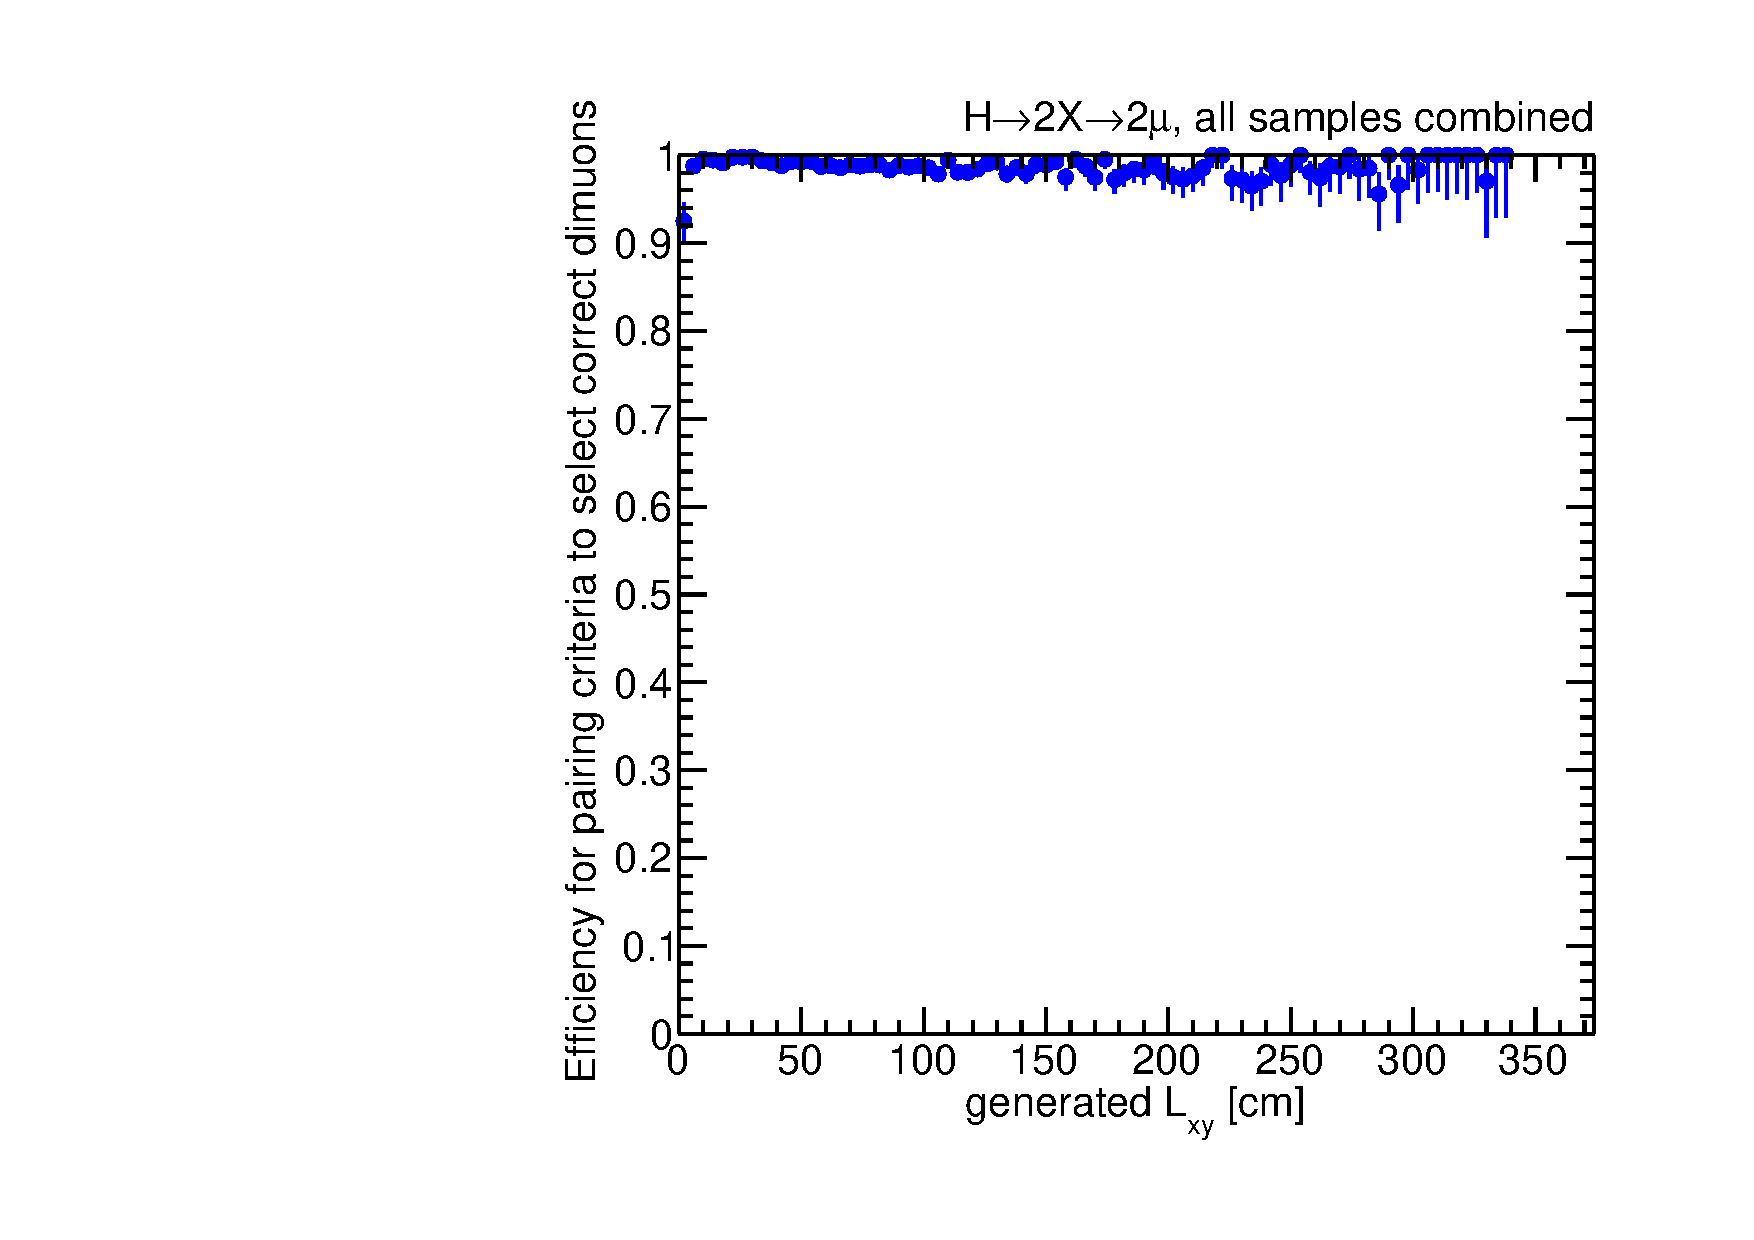
\includegraphics[width=\DSquareWidth]{figures/displaced/PC_Lxy_2Mu2J_Global.pdf}
  \hspace*{-2em}
  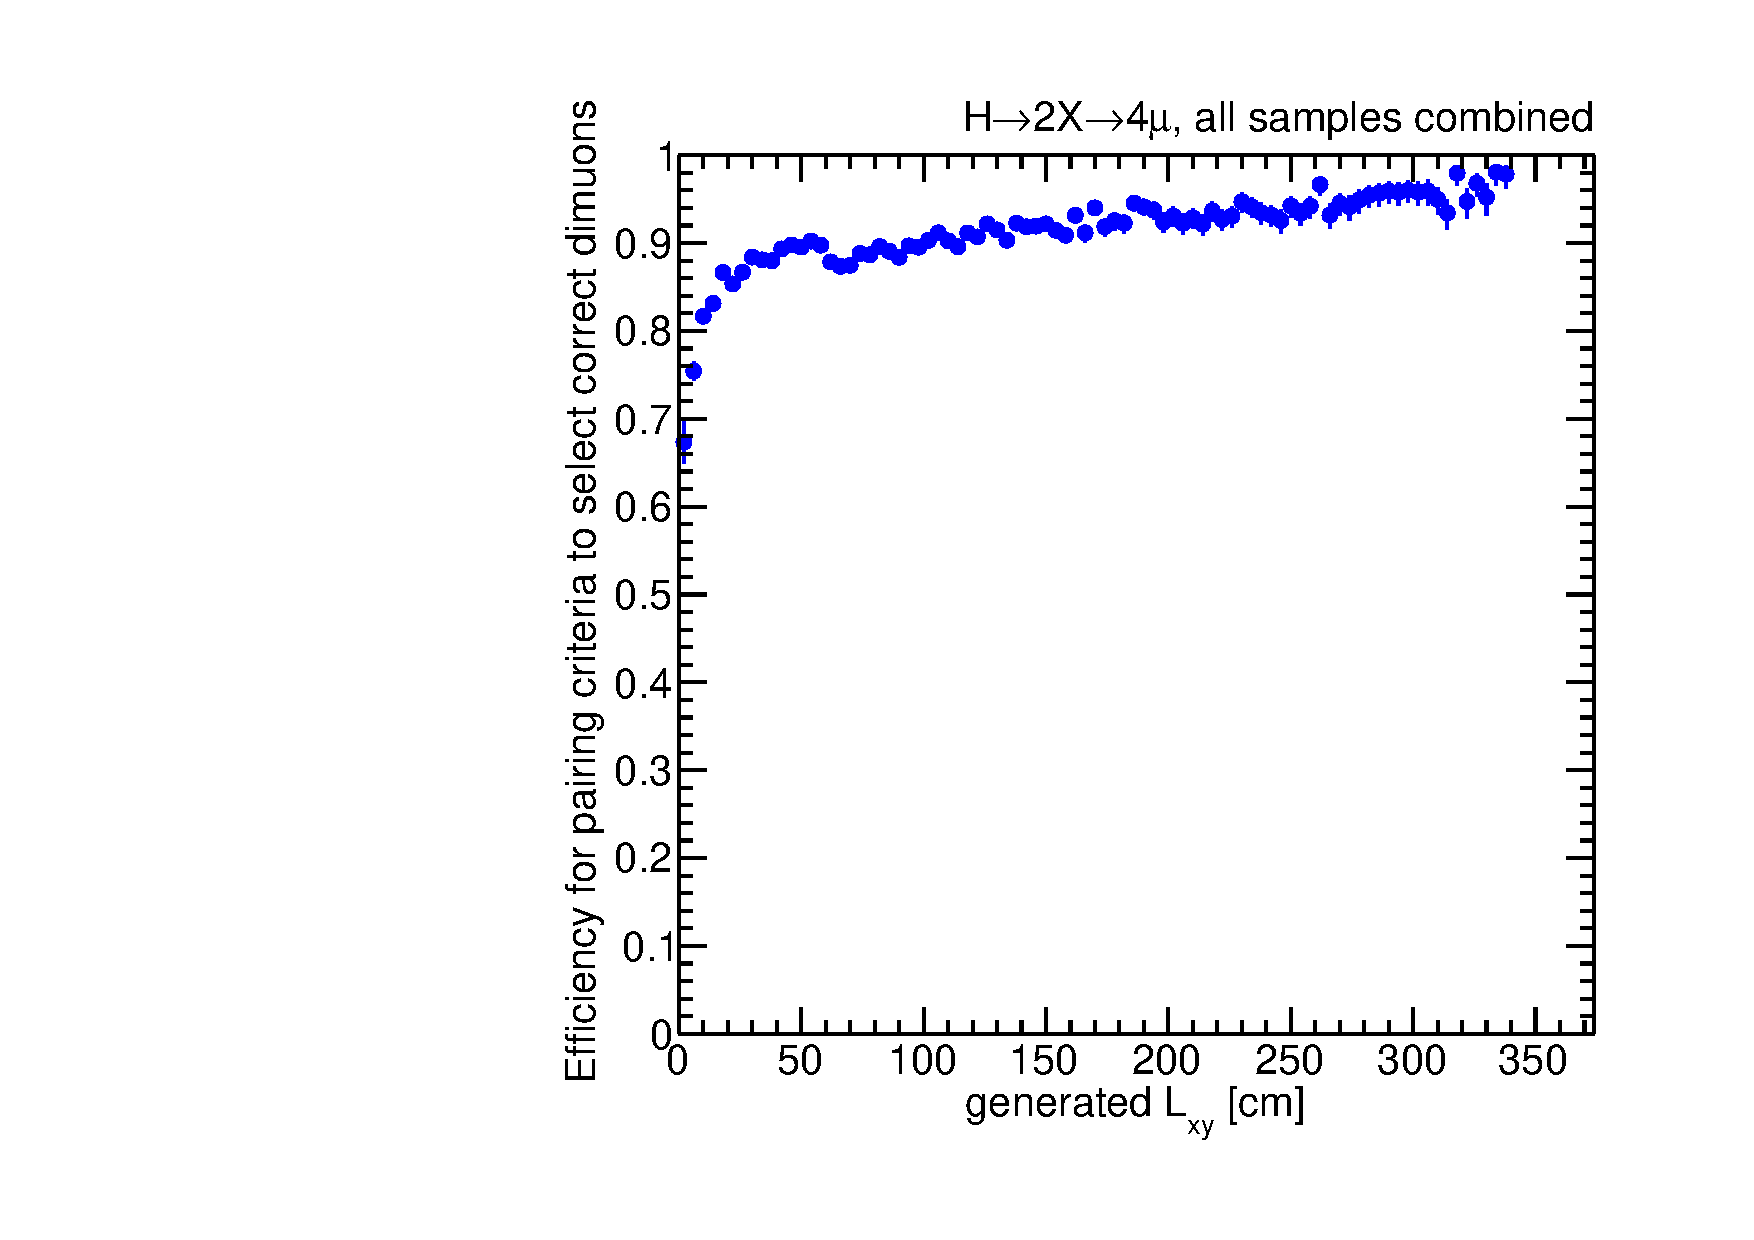
\includegraphics[width=\DSquareWidth]{figures/displaced/PC_Lxy_4Mu_Global.pdf}
  \caption[Efficiency for the pairing criteria to correctly choose reconstructed dimuons.]{Efficiency for the pairing criteria to correctly choose reconstructed dimuons, as in \Fig~\ref{fig:dd:PC_Eff}, for all samples combined.}
  \label{fig:dd:PC_Eff_Global}
\end{figure}

\subsection{Dimuon Object Selection}
\label{sec:dd:DimuonObject}
Along with the DCA requirement, the requirement of convergence of the common vertex fit, and the application of the pairing criteria explained in \Sec~\ref{sec:dd:PC}, the following requirements serve as a dimuon identification selection.
These requirements further select high-quality dimuons as well as suppress background events.
Dimuons are required:
\begin{itemize}
  \item to have a reconstructed dimuon mass of at least 10\GeV, \ie $\mMuMu > 10\GeV$
  \item to have a $\chi^2$ of the common vertex fit of at most 20, \ie $\chi^2_\text{vertex} < 20$
\end{itemize}

The \vchisq cut ensures that the dimuon is formed from tracks that can be reasonably well associated with a common vertex.
The mass cut suppresses complex backgrounds arising from QCD processes and events with low \pT and collimated muons.

\subsection{Dimuon Signal Selection}
\label{sec:dd:DimuonSignal}
The following criteria select displaced dimuons consistent with the signal hypothesis, \ie that the dimuon was constructed from two muons with opposite-sign charge originating from the decay of a long-lived particle produced promptly, resulting in a dimuon vertex displaced from the beam spot.
The relevant quantities were defined in \Sec~\ref{sec:dd:keyvars}.
Dimuons are required:
\begin{itemize}
  \item to have an \Lxy significance of at least 6, \ie $\LxySig > 6$
  \item to have a transverse collinearity angle of less than $\pi/4$, \ie $\DeltaPhi < \pi/4$
  \item to be formed from two DSA muons with electric charges of opposite sign
\end{itemize}

\subsection{Cosmic Muon Suppression}
\label{sec:dd:CosmicCuts}
As mentioned in \Sec~\ref{sec:dd:VertexFitting}, one result of the common vertex fit of two muons is a pair of vertex-constrained tracks.
After the common vertex fit, a population of selected dimuons with relatively small \vchisq values was observed in data, and not in simulation, with the following unusual properties, compared to before the common vertex fit:
\begin{itemize}
  \item Muon vertex-constrained momentum $\phi$ directions change by approximately $\pi$
  \item Muon vertex-constrained \pT uncertainties are unusually small, \ie $\pTErr/\pT \approx 10^{-7}\text{--}10^{-5}$
\end{itemize}
The presence of these dimuons are found to correlate with
\begin{itemize}
  \item Muons with relatively large transverse impact parameters, \ie $d_0 \approx 200\text{--}1000\cm$, and
  \item Events with no \pp collision vertices, and/or
  \item Events with large numbers of DSA muons, \ie $N(\text{DSA}) \approx 15\text{--}20$
    \begin{itemize}
      \item And these large numbers of DSA muons are largely parallel, \ie $|\cos{\alpha}| \approx 1$
    \end{itemize}
\end{itemize}
Further investigation suggested that these events are consistent with showers of cosmic muons.
\Fig~\ref{fig:dd:shower} is an example display of an event in data consistent with a shower of cosmic muons in a \pp collision event, containing a large number of approximately parallel pairs of DSA muons in addition to two global muons (not selected) originating from the \pp collision.

\begin{figure}[htpb]
  \centering
  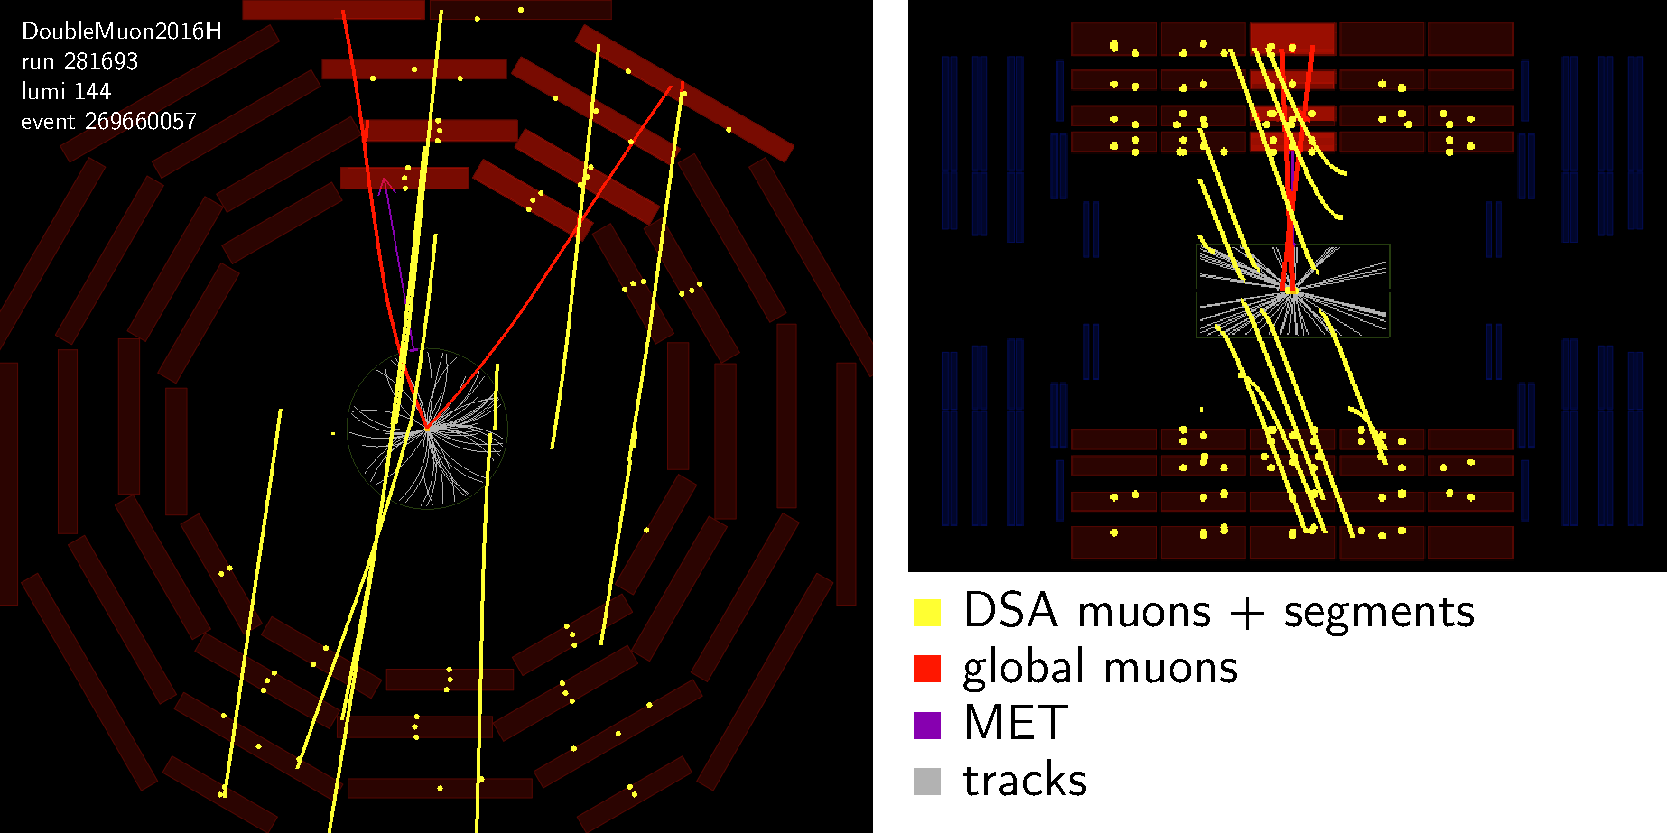
\includegraphics[width=\textwidth]{figures/displaced/ED_Cosmic.pdf}
  \caption[Display of an event in data consistent with a shower of cosmic muons in a \pp collision event.]{Display of an event in data consistent with a shower of cosmic muons in a \pp collision event. Two of the many approximately parallel DSA muons (yellow) reconstructed in this event formed a dimuon vertex with a good \vchisq and the event subsequently passed all our other selections. Requirements that events not contain too many parallel pairs of DSA muons and that the opening angle between the two muons not be too close to $\pi$ were found to be effective in suppressing such events.}
  \label{fig:dd:shower}
\end{figure}

A cosmic muon can be reconstructed as two back-to-back muons, one in the upper half of the detector and one in the lower half of the detector.
A reconstructed dimuon could also be formed from half a cosmic muon and a track from the \pp collision.
These dimuons are reconstructed as highly displaced, which is why the muons have such large $d_0$ values.
The common vertex fit discussed above has anomalous behavior at large displacements, so the presence of the flip-by-$\pi$ and small \pT uncertainty anomalies when fitting to muons with large $d_0$ is perhaps not unexpected.
Such events are background events and so the analysis imposes a set of selections designed to suppress showers of cosmic muons.

Some of these events have no \pp collision vertices and contain only cosmic muons.
Events are therefore required to contain at least one well-identified vertex with position $(x, y, z)$ satisfying the following requirements:
\pagebreak
\begin{itemize}
  \item At least 4 degrees of freedom when constructing the vertex
  \item $|z| < 24\mm$
  \item $\sqrt{x^2 + y^2} < 2\mm$
\end{itemize}
This set of requirements is referred to in CMS as the \Code{PrimaryVertexFilter}.

A typical strategy to suppress back-to-back cosmic muons is with a selection on $\cos{\alpha}$, and indeed the trigger has just such a cut, roughly equivalent to $\cos{\alpha} > -0.8$.
Following the trigger, our offline analysis selection also requires $\cos{\alpha} > -0.8$, on the opening angles both between the vertex-constrained muons and between the original (before the vertex fit) muons.

However, these two requirements alone are not sufficient to suppress all events consistent with cosmic muon showers.
As an additional measure to suppress cosmic muon showers, the analysis rejects events with a large number of parallel pairs of DSA muons.
All possible pairs of DSA muons, with no common vertex fit, are considered, and the number $N(\text{parallel pairs})$ of such pairs with $|\cos{\alpha}| > 0.99$ are counted.
The analysis selection then requires that events contain no more than 5 such pairs, verified to be of negligible efficiency in signal.

In summary, the cosmic muon suppression selections are
\begin{itemize}
  \item Events pass the \Code{PrimaryVertexFilter}
  \item Events have $N(\text{parallel pairs}) < 6$
  \item Dimuons have original and vertex-constrained $\cos{\alpha} > -0.8$
\end{itemize}

\subsection{Summary of Event and Object Selection}
\Tab~\ref{tab:dd:fullsel} summarizes the full event and object selections discussed in this section.
When setting upper limits, the mass cut is further varied as a function of signal model, as explained in \Sec~\ref{sec:dd:cutopt_mass}.
\begin{table}
  \centering
  \begin{tabular}{llll} 
    \hline\hline
    \multicolumn{4}{c}{Event Selection} \\
    \hline
    primary vertex                    & \multicolumn{3}{l}{\Code{PrimaryVertexFilter} passed}       \\
    HLT-RECO matching                 & \multicolumn{3}{l}{HLT-RECO matching algorithm found match} \\
    number of parallel DSA muon pairs & $N$(parallel pairs) & $<$ & 6                               \\
    \hline
    & & \\

    \hline\hline
    \multicolumn{4}{c}{DSA Muon Selection} \\
    \hline
    association with PAT muons         & \multicolumn{3}{l}{DSA muons \emph{not} associated with PAT muons}  \\
    number of CSC and DT stations      & $N$(CSC+DT stations)                      & $>$ & 1               \\
    number of CSC and DT hits          & $N$(CSC+DT hits)                          & $>$ & 12              \\
    number of DT hits for barrel muons & $N(\text{DT hits}\,\vert\,\text{barrel})$ & $>$ & 18              \\
    relative \pT uncertainty           & $\pTErr/\pT$                              & $<$ & 1               \\
    transverse muon momentum           & \pT                                       & $>$ & 10\GeV          \\
    normalized track \normchisq        & $\chisq_\text{track}/\text{dof}$          & $<$ & 2.5             \\
    time at interaction point          & $|t_\text{in-out}|$                       & $<$ & 12\unit{ns}     \\
    \hline
    & & \\

    \hline\hline
    \multicolumn{4}{c}{Dimuon Selection} \\
    \hline
    distance of closest approach of muon & DCA                            & $<$ & 50\cm          \\
    common vertex fit                    & \multicolumn{3}{l}{common vertex fit converged}       \\
    pairing criteria                     & \multicolumn{3}{l}{best 1--2 ranked dimuons selected} \\
    dimuon mass                          & $\mMuMu$                       & $>$ & 10\GeV*        \\
    vertex \chisq                        & $\chisq_\text{vertex}$         & $<$ & 20             \\
    cosine of dimuon 3D opening angle    & $\cos{\alpha}$                 & $>$ & $-0.8$         \\
    \Lxy significance                    & \LxySig                        & $>$ & 6              \\
    transverse collinearity angle        & \DeltaPhi                      & $<$ & $\pi/4$        \\
    opposite sign muons                  & \multicolumn{3}{l}{constituent muons are oppositely charged} \\
    \hline
  \end{tabular}
  \caption[Summary of full selection, organized into event, muon, and dimuon requirements.]{Summary of full selection, organized into event, muon, and dimuon requirements. The asterisk refers to a selection that varies depending on the signal model used; see \Sec~\ref{sec:dd:cutopt_mass}.}
  \label{tab:dd:fullsel}
\end{table}

\section{Background Estimation}
\label{sec:dd:bgest}
As mentioned above, due to MC simulation limitations, evaluating the expected background in the selection is performed using events in data.
To avoid potential bias while optimizing the analysis, the events passing the full selection in data (the signal region) were blinded until the last steps of the analysis, and the background was estimated using the numbers of events in data in several control regions, which are selections (in the parameter space of the analysis quantities) of subsets of events that are expected to be free of signal events.

As discussed in \Sec~\ref{sec:dd:timing}, after unblinding there was a change made to the selection, notably rejection of a clear class of background events with bad timing.
We also realized that same-sign events could be put to better use in quantitative estimates of the opposite-sign background from QCD events, beyond the rough qualitative use that we had foreseen.

One type of control region is defined as an interval of the transverse collinearity angle, \DeltaPhi.
As discussed in \Sec~\ref{sec:dd:keyvars}, the signal and background have different distributions in \DeltaPhi.
For dimuons consistent with the signal hypothesis, the dimuon momentum vector should be consistent with a particle originating from the primary vertex, and so \DeltaPhi is expected to be small, peaking at zero.
\Fig~\ref{fig:dd:deltaPhi_Sig} shows the distribution of \DeltaPhi for \twoMu signal events (all 33 sets of signal parameters combined) passing the full selection (as described in the previous section), except for the \DeltaPhi cut.

\begin{figure}[htpb]
  \centering
  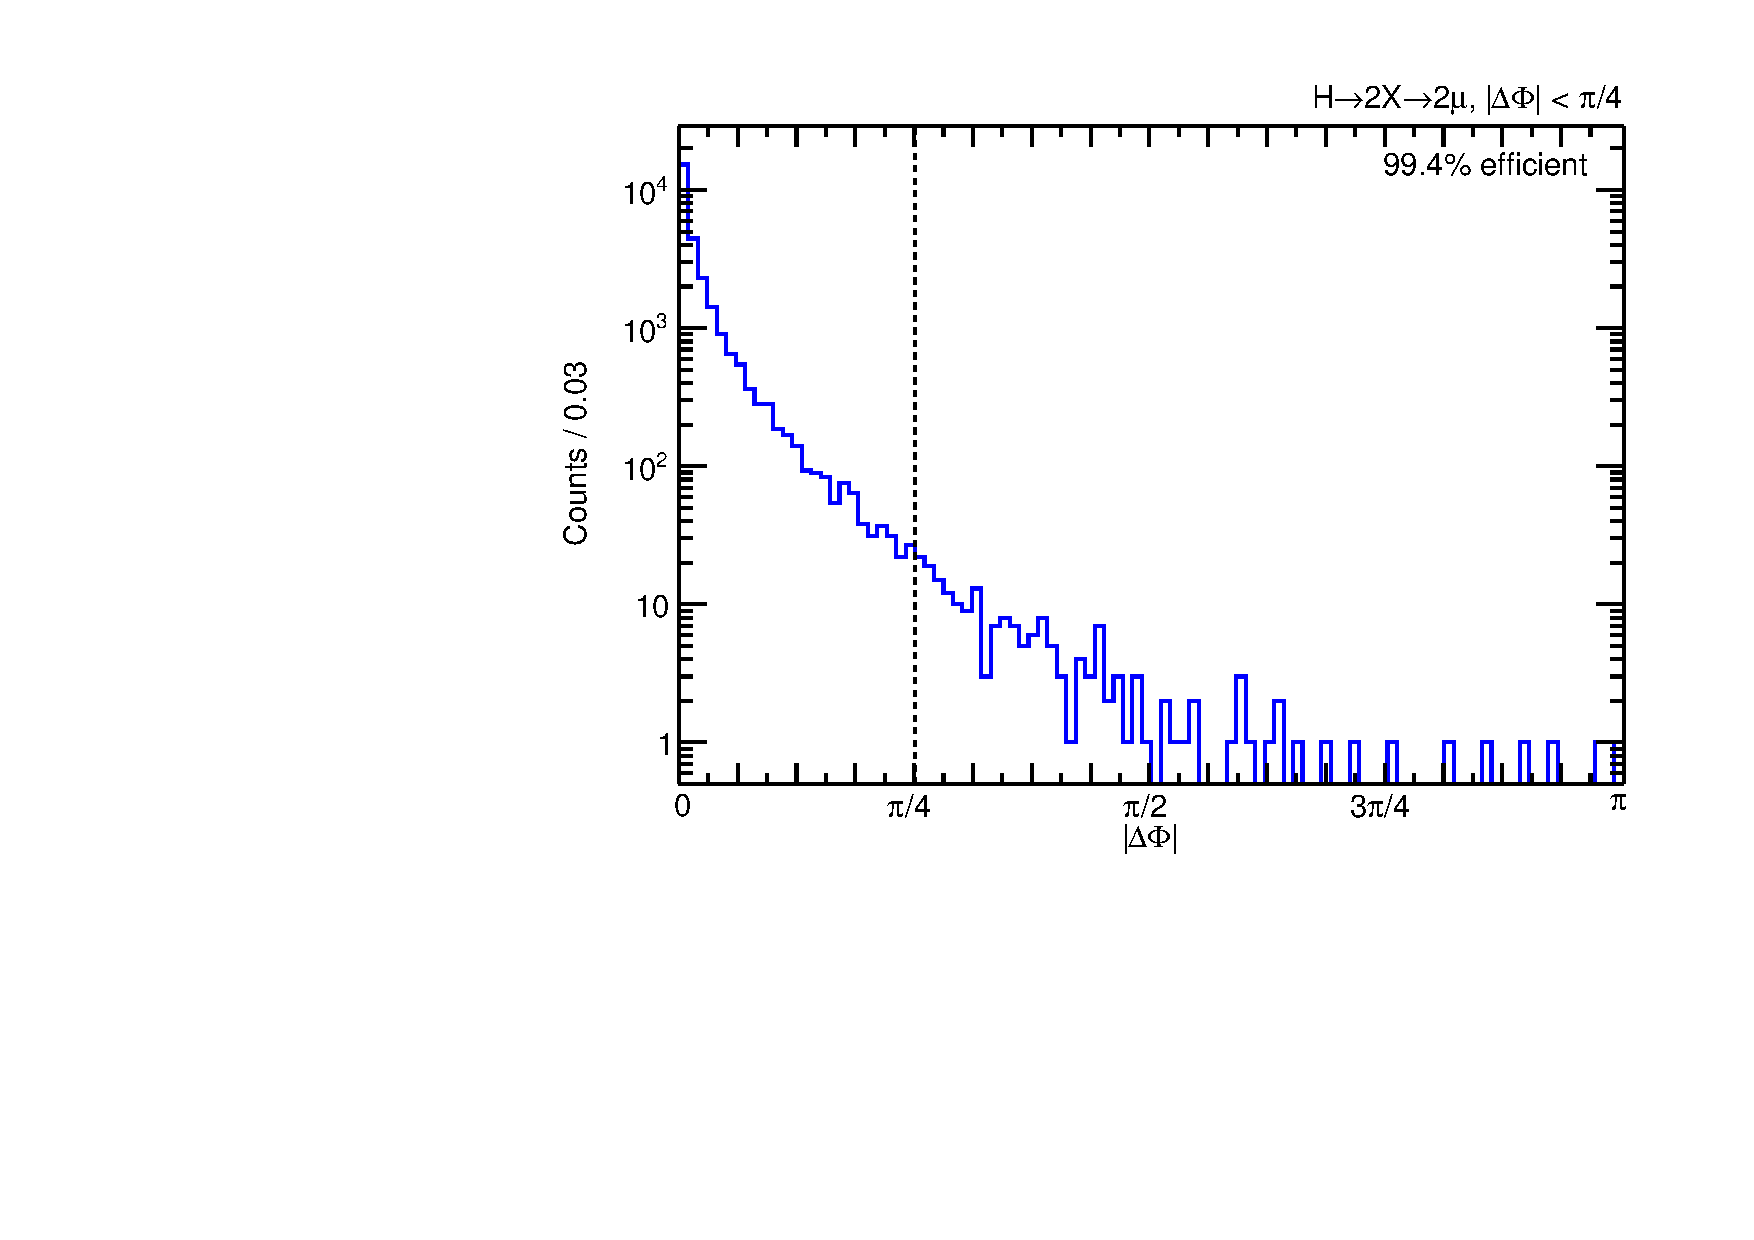
\includegraphics[width=\DFigWidth]{figures/displaced/NM1_2Mu2J_deltaPhi.pdf}
  \caption[Histogram of \DeltaPhi for all \twoMu simulated signal samples combined, showing a strong peak at zero.]{Histogram of \DeltaPhi for all \twoMu signal samples combined, showing a strong peak at zero. The dashed line is at $\DeltaPhi = \pi/4$; the cut $\DeltaPhi < \pi/4$ is 99.4\% efficient in signal.}
  \label{fig:dd:deltaPhi_Sig}
\end{figure}

On the other hand, dimuons in some background events, such as misreconstructed Drell-Yan events, are expected to have a \DeltaPhi distribution symmetric around $\pi/2$, because the dimuon momentum vector is uncorrelated with the direction of flight from the primary vertex.
This expected symmetry of \DeltaPhi motivates the definition of the signal region as events with \DeltaPhi near 0, \ie $\DeltaPhi < \pi/4$ and a symmetric control region as events with \DeltaPhi near $\pi$, \ie $\DeltaPhi > 3\pi/4$.
A transfer factor (\TF) is defined as the ratio between the number of events in the signal region to the control region.
With $\TF = 1$, the number of events in the control region is a nominal estimate of the expected (Drell-Yan) background in the signal region.

\pagebreak
To validate the approximate background symmetry around $\pi/2$ (and better quantify the transfer factor), the analysis considers pairs of control regions that include the regions $\DeltaPhi < \pi/4$ or $\DeltaPhi > 3\pi/4$ but are formed by reversing other selections (discussed below).

\subsection{Notation for Control Regions}
One set of DSA dimuon control events is obtained by reversal of the \LxySig selection, so that events have small \LxySig instead, \eg $\LxySig < 6$.
Another set of DSA dimuon events are obtained by reversal of the opposite-sign charge selection, so that dimuons consist of muons reconstructed with the same sign.

A final set of DSA dimuon events are obtained by reversal of \DSAToPAT association.
This set consists of DSA dimuons (formed from two DSA muons), passing all selections except for the \DSAToPAT association procedure, in which the two constituent DSA muons can be associated with two PAT muons, and the resulting dimuon formed from two PAT muons has its own PAT \LxySig satisfying a certain range.

Two such ranges are used in this section.
In the first, the PAT \LxySig is small, \eg $\LxySig < 1$.
This region is designed to study Drell-Yan background, and corresponds to DSA dimuons whose PAT muon counterparts are consistent with being produced promptly (and thus are not signal), but which may be reconstructed as highly displaced due to reconstruction mistakes or vertex fit anomalies.
In order to minimize contamination from QCD events, each constituent muon is required to be isolated.
The relative isolation of a muon track is defined as the scalar sum of the \pT of tracks in a \DeltaR cone around the muon divided by the muon \pT.
For this first range, the relative isolation of each constituent PAT muon is required to be at most 0.05.

In the second range, the PAT \LxySig is large, such as \mbox{$60 < \LxySig < 115$}.
This region is designed to study QCD background, such as from cascade decays of $b$ to $c$ quarks or hadrons in flight.
In order to minimize signal contamination, each constituent PAT muon is required to \emph{not} to be isolated, meaning the relative isolation of each constituent PAT muon is required to be at least 0.5.
Less than 3\% of \twoMu signal events satisfy this non-isolation requirement, which meanwhile selects a subset of events composed of approximately 95\% events from QCD processes (according to MC simulation).

With any combination of these three reversals, a pair of control regions may be formed satisfying $\DeltaPhi < \pi/4$ or $\DeltaPhi > 3\pi/4$, respectively.

Some tedious notation is introduced to facilitate discussion of the various control regions.
These regions are labeled CR with the following sublabels:
\begin{itemize}
  \item The superscript on the left side of CR is either 0, 1, 2, or $\pi$, corresponding respectively to the \DeltaPhi ranges $0 < \DeltaPhi < \pi/4$, $\pi/4 < \DeltaPhi < \pi/2$, $\pi/2 < \DeltaPhi < 3\pi/4$, and $3\pi/4 < \DeltaPhi < \pi$.
  \item The subscript on the left side of CR is either OS or SS, corresponding respectively to DSA dimuons consisting of muons with charges of \textbf{o}pposite \textbf{s}ign and muons with charges of the \textbf{s}ame \textbf{s}ign.
  \item The superscript on the right side of CR is of the format $L<x$ or $L>x$ with $x$ a cut value, usually 6, corresponding to DSA dimuons with a reversed \LxySig selection, as described above. This label means that \LxySig value for the dimuon formed from two DSA muons is less than $x$ or greater than $x$. The $L$ in this expression is a reminder that the cut value is for \LxySig.
  \item The subscript on the right side of CR is one of
    \begin{itemize}
      \item $P(\mathrm{full})$, corresponding to a control region in which the full, standard \DSAToPAT association is performed;
      \item $P(D)$, corresponding to the DSA dimuons with reversed \DSAToPAT association as described above with the PAT dimuon satisfying $\LxySig < 1$ and muons isolated; or
      \item $P(Q)$, corresponding to the DSA dimuons with reversed \DSAToPAT association as described above with the PAT dimuon satisfying $60 < \LxySig < 115$ and muons not isolated.
    \end{itemize}
    The DSA dimuon passes the selections on \DeltaPhi and \LxySig given by the other two labels. The $D$ and $Q$ in these expressions are abbreviations for the type of background, either \textbf{D}rell-Yan or \textbf{Q}CD, that these control regions are designed to help estimate; the PAT \LxySig ranges were chosen accordingly.
\end{itemize}
For example, \CR[OS]{D}{<6}{\pi} corresponds to opposite-sign DSA dimuons with \mbox{$\DeltaPhi > 3\pi/4$}, DSA $\LxySig < 6$, and reversed \DSAToPAT association with PAT $\LxySig < 1$.
The signal region SR consisting of DSA dimuons passing all selections can be expressed in this notation as $\mathrm{SR} \equiv\, \CR[OS]{\Full}{>6}{0}$.

\subsection{Estimation of Drell-Yan Background}
\label{sec:dd:bgest-DY}
Misreconstructed Drell-Yan events form a large majority of the background in most regions.
\Fig~\ref{fig:dd:BGDeltaPhi_NoPAT} shows distributions of \DeltaPhi in data and in MC simulation for the control regions with \DSAToPAT association reversed, for all ranges of \DeltaPhi.
The left plot is for all values of \LxySig; that is, it contains both \CR{D}{>6}{} and \CR{D}{<6}{} for all \DeltaPhi ranges $(0, 1, 2, \pi)$.
The right plot is only for $\LxySig > 6$; that is, it only contains \CR{D}{>6}{} for all \DeltaPhi ranges.
Without any \LxySig cut, the distribution is somewhat symmetric, with some excess of events at $\pi$ compared to 0.
With the \LxySig cut, events at 0, $\pi/2$, and $\pi$ are suppressed less than other events, although the distributions are still fairly symmetric.

\begin{figure}[t]
  \centering
  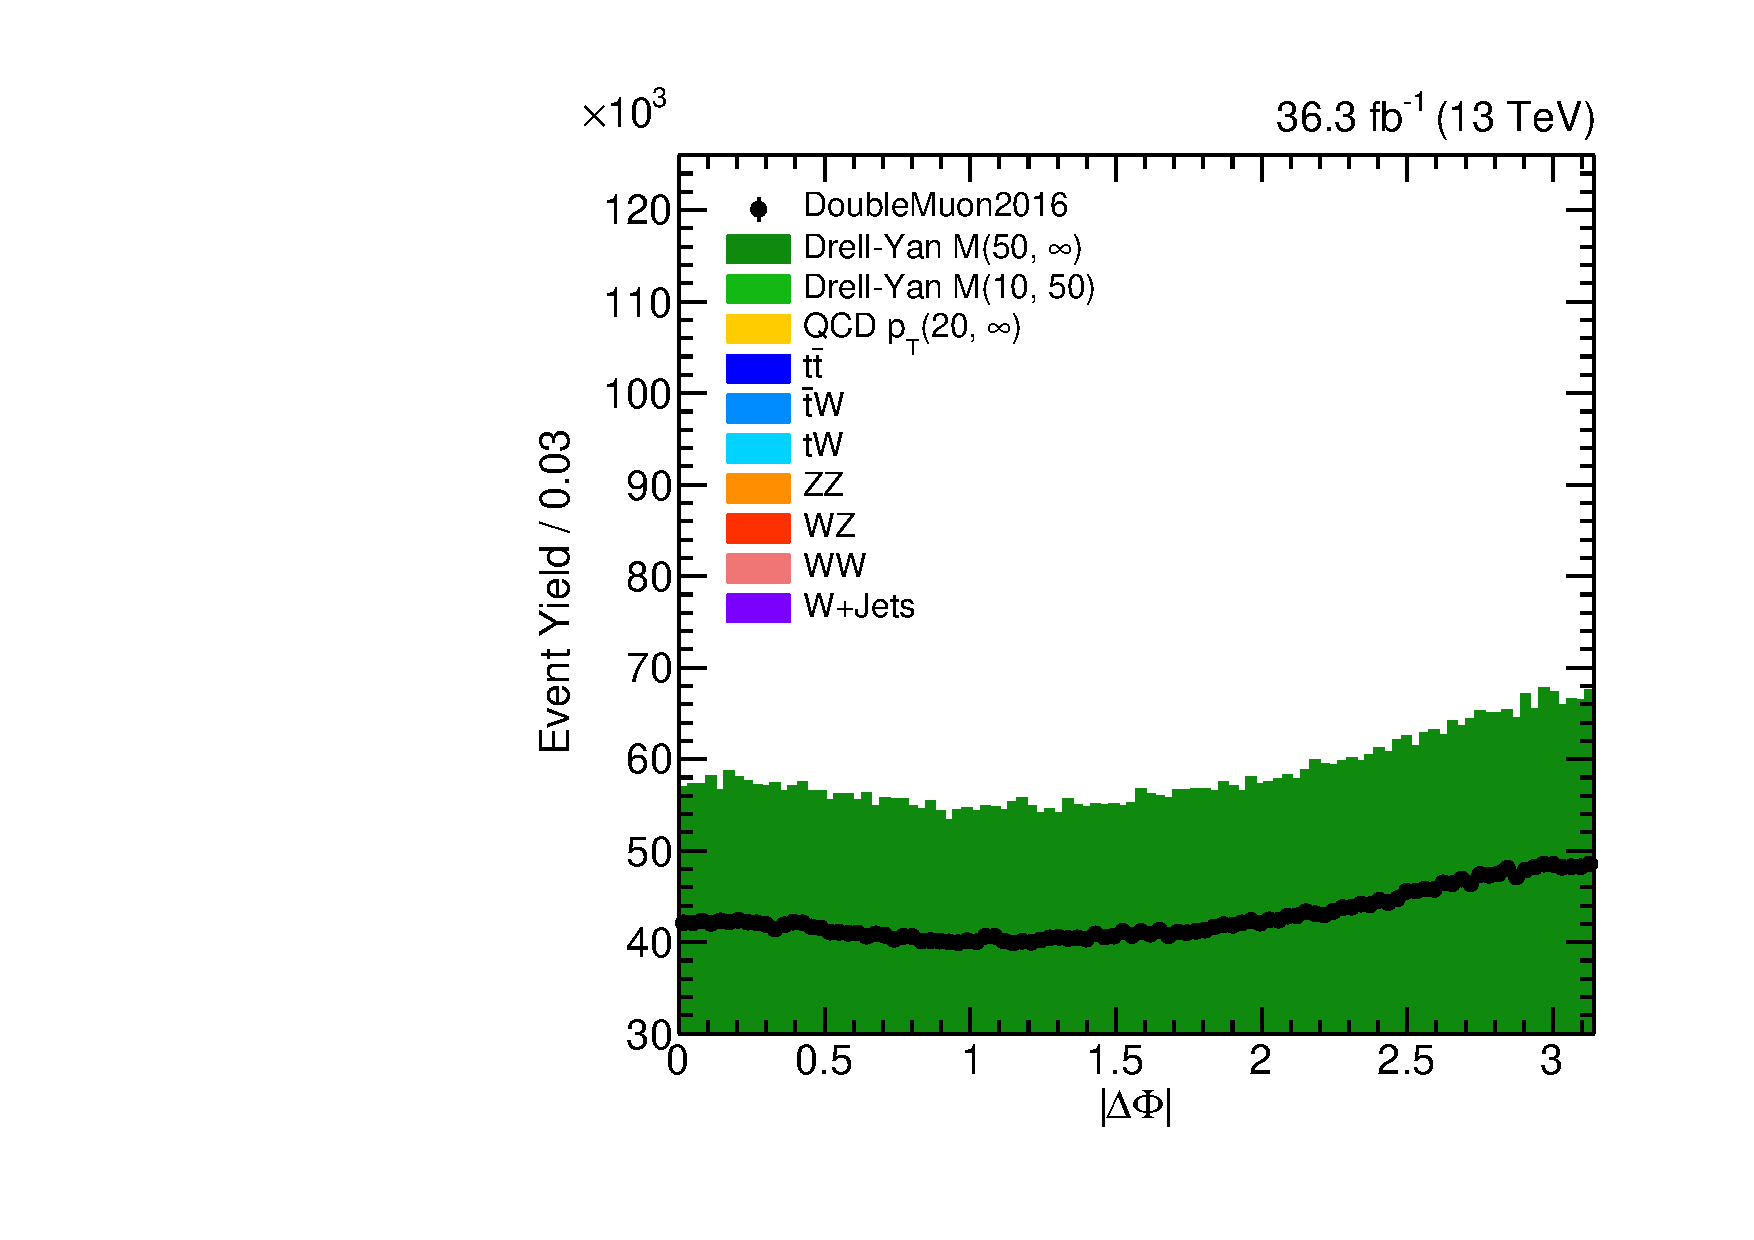
\includegraphics[width=\DSquareWidth]{figures/displaced/BGEST_NOPAT_deltaPhi_Lin.pdf}
  \hspace*{-2em}
  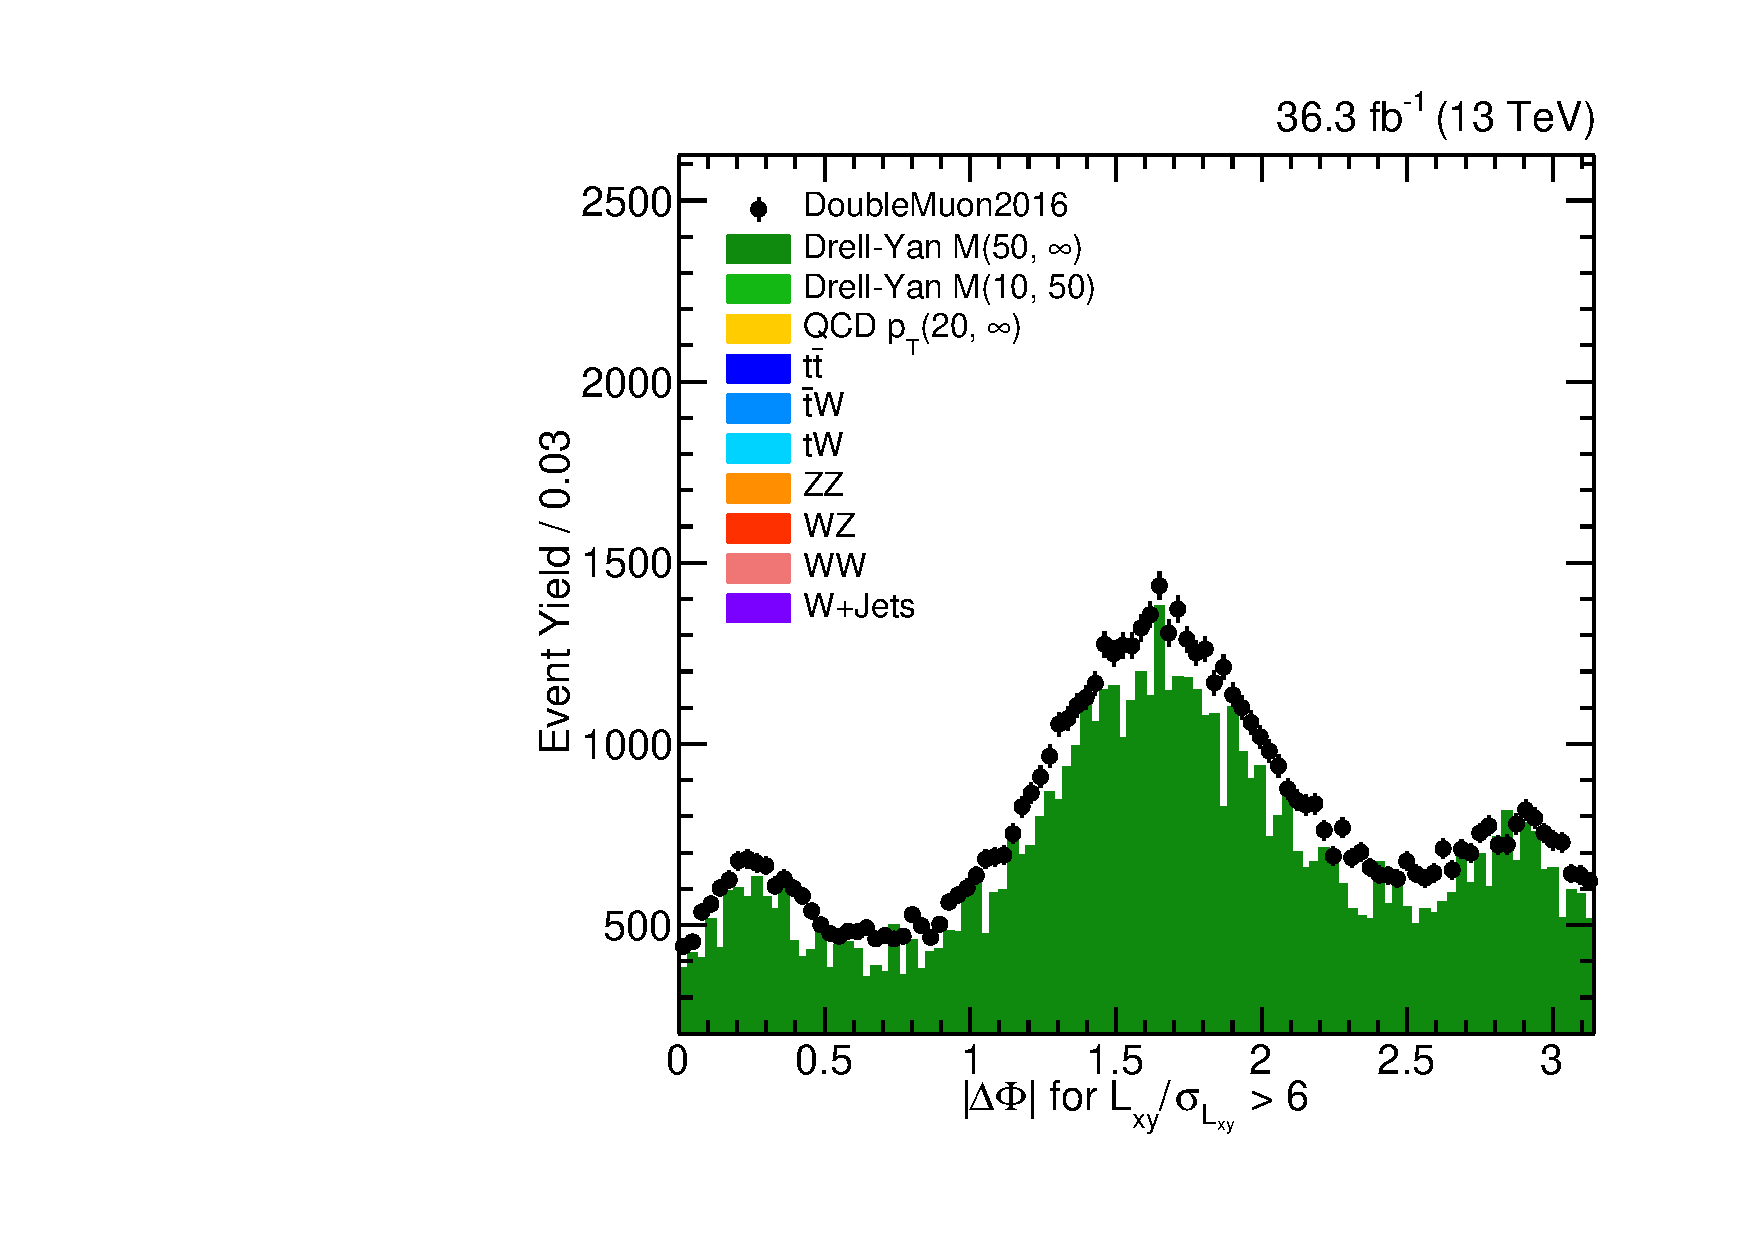
\includegraphics[width=\DSquareWidth]{figures/displaced/BGEST_NOPAT_deltaPhi-Big_Lin.pdf}
  \caption[Histograms of \DeltaPhi in data and in MC simulation for the control regions with \DSAToPAT association reversed, for all values of \DeltaPhi, for all values of \LxySig and for $\LxySig > 6$.]{Histograms of \DeltaPhi in data and in MC simulation for the control regions with \DSAToPAT association reversed, for all values of \DeltaPhi, for \figpos{left} all values of \LxySig and \figpos{right} only $\LxySig > 6$. In the previously introduced notation, \figpos{right} consists of \CR{D}{>6}{0}, \CR{D}{>6}{\pi}, \etc, and \figpos{left} consists of all the events in the right plot plus \CR{D}{<6}{0}, \CR{D}{<6}{\pi}, \etc Without any \LxySig cut, the distribution is somewhat symmetric, with some excess of events at $\pi$ compared to 0. With the \LxySig cut, events at 0, $\pi/2$, and $\pi$ are suppressed less than other events, although the distributions are still fairly symmetric.}
  \label{fig:dd:BGDeltaPhi_NoPAT}
\end{figure}

Understanding this shape begins by considering Drell-Yan events, which compose a majority of the background, and for which the event geometry often consists of two back-to-back muons.
These muons' directions are often well reconstructed, whereas their \pT may not be, resulting in the dimuon \pT pointing along the direction of one of the muons.
With this event topology in mind, the shape can be explained by the combination of two effects.

The first effect is a result of the decrease in trigger efficiency for large transverse impact parameters $d_{0}$.
Events in which the muon tracks are parallel to the \Lxy vector are events in which the muons point towards the primary vertex, so that their $d_0$ is small.
Events in which the muon tracks are perpendicular to the \Lxy vector are events with large transverse impact parameters, and would be suppressed by the trigger.
But the dimuon \pT is along the direction of one of the muons, so parallel muon tracks correspond to $\DeltaPhi \approx 0$ (or $\pi$), while perpendicular muon tracks correspond to $\DeltaPhi \approx \pi/2$.
In other words, large values of \Lxy only pass the trigger when the muons sufficiently point towards the primary vertex, \ie have $\DeltaPhi \approx 0$ (or $\pi$), effectively suppressing $\DeltaPhi \approx \pi/2$.

(As a thought experiment, consider muons moving in the detector with no magnetic field. Then $d_0 = \Lxy \sin{\DeltaPhi}$.
If the trigger efficiency sharply vanished at some fixed value $d_0 \geq D$, then only events with $\Lxy \leq D \csc{\DeltaPhi}$ would pass the trigger.
Cosecant takes large values around $\DeltaPhi = 0$ and $\DeltaPhi = \pi$, and small values at $\DeltaPhi = \pi/2$.
The diagram in the top row of \Fig~\ref{fig:dd:BGEST_WavyExplanationDiagram} illustrates this first effect in the context of this thought experiment.)

The second effect is a result of geometric effects on the uncertainty of the position of the fitted vertex.
For back-to-back muons, the uncertainty on the fitted dimuon vertex is larger along the direction of the tracks than orthogonal to it, because the uncertainty orthogonal to the track is set by the scatter of hits about the tracks, whereas determining the position of the vertex along two back-to-back tracks is more difficult.
Then for a given \Lxy, the uncertainty on \Lxy, \LxyErr, is larger when the muons (and hence the dimuon \pT) are parallel to the \Lxy vector (\ie $\DeltaPhi = 0$ or $\pi$) and smaller when the muons (and hence the dimuon \pT) are perpendicular to the \Lxy vector (\ie $\DeltaPhi = \pi/2$).
In other words, \LxyErr is smaller at $\pi/2$ than at 0 or $\pi$.
The diagrams in the bottom row of \Fig~\ref{fig:dd:BGEST_WavyExplanationDiagram} illustrate this second effect.

\begin{figure}[htpb]
  \centering
  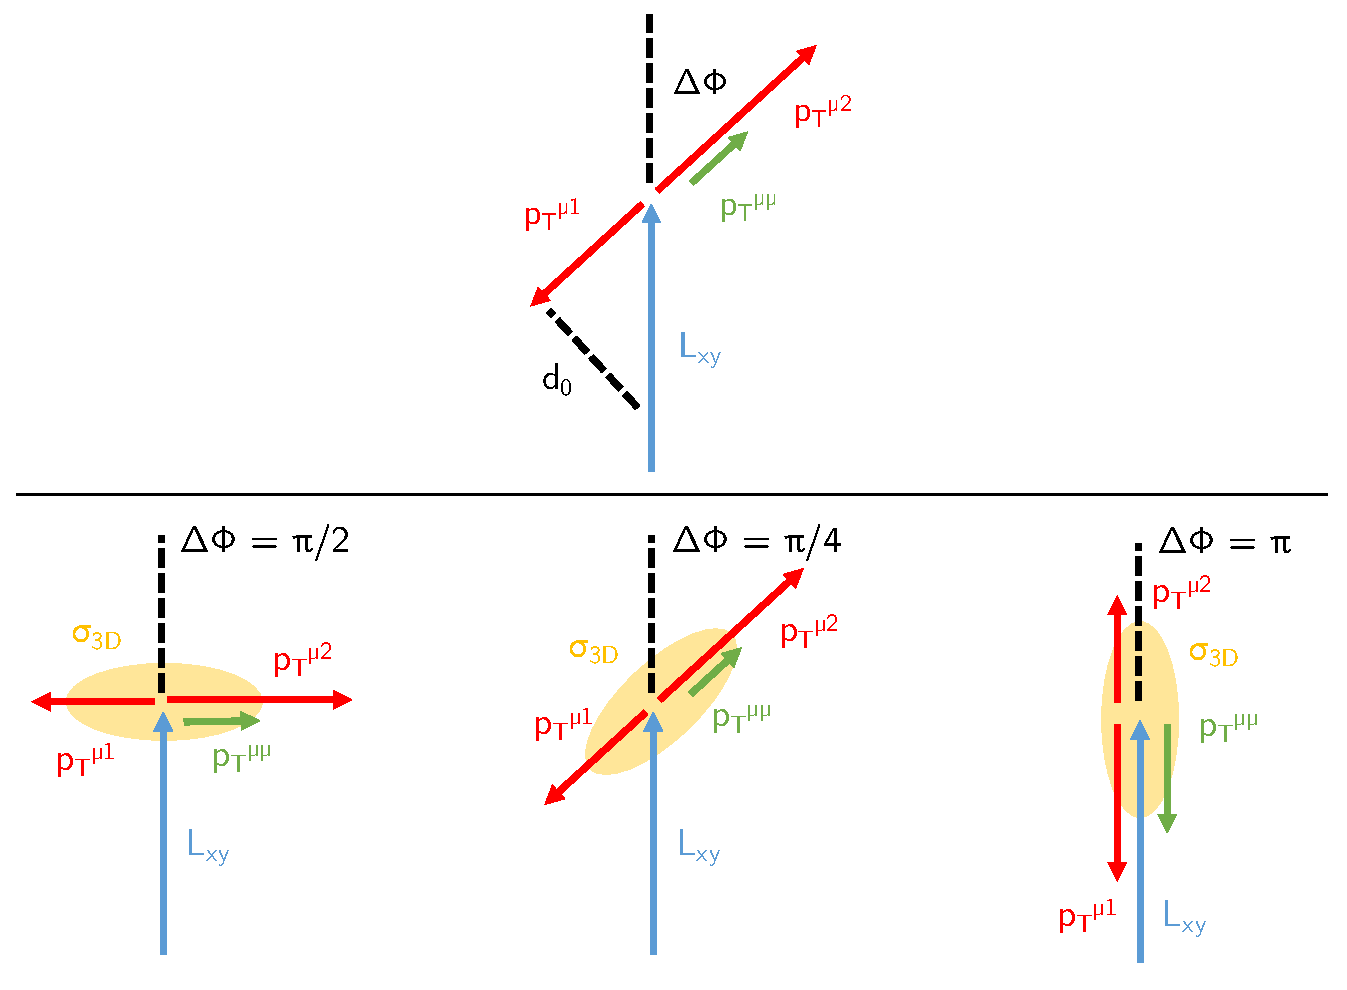
\includegraphics[width=1.2\DFigWidth]{figures/displaced/BGEST_WavyExplanationDiagram.pdf}
  \caption[Diagrams depicting the effect of dimuon orientation on possible values of \Lxy and \LxyErr.]{\figpos{Top} Diagram depicting the effect of dimuon orientation on possible values of \Lxy. Lowered trigger efficiency at large transverse impact parameter ($d_0$) values suppresses large \Lxy values, which have significant $d_0$ unless \DeltaPhi is sufficiently close to 0 or $\pi$. \figpos{Bottom} Diagram depicting the effect of dimuon orientation on \LxyErr as a function of \DeltaPhi. The dimuon \pT points along one of the muons, which are back-to-back, and the uncertainty on the position of the fitted vertex is represented by a yellow ellipse around the vertex, with the larger axis parallel to the muon. For a given \Lxy the \LxyErr is larger when the muons are parallel to the \Lxy vector (\ie $\DeltaPhi = 0$ or $\pi$) and smaller when the muons are perpendicular to it (\ie $\DeltaPhi = \pi/2$), taking an intermediate value with $\DeltaPhi = \pi/4$ (or $3\pi/4$).}
  \label{fig:dd:BGEST_WavyExplanationDiagram}
\end{figure}

A selection on \LxySig selects events with large \Lxy and/or small \LxyErr, which have been shown to preferentially occur at 0, $\pi/2$, and $\pi$.
The resulting shape of the \DeltaPhi distribution appears to be geometric in origin, and is the motivation for defining the signal and control regions as $\DeltaPhi < \pi/4$ and its symmetric region around $\pi/2$, in order to cut away from the extra background at $\pi/2$.
\Fig~\ref{fig:dd:SeqLxySig} shows the $\DeltaPhi$ distributions as in the right plot of \Fig~\ref{fig:dd:BGDeltaPhi_NoPAT}, each scaled to unit area, for data and for Drell-Yan simulation, for sequentially increasing cuts on \LxySig (\ie \CR{D}{>x}{} for all \DeltaPhi and $x$ variable).
The Drell-Yan plot indicates that the shape is well-reproduced by simulation.

\begin{figure}[t]
  \centering
  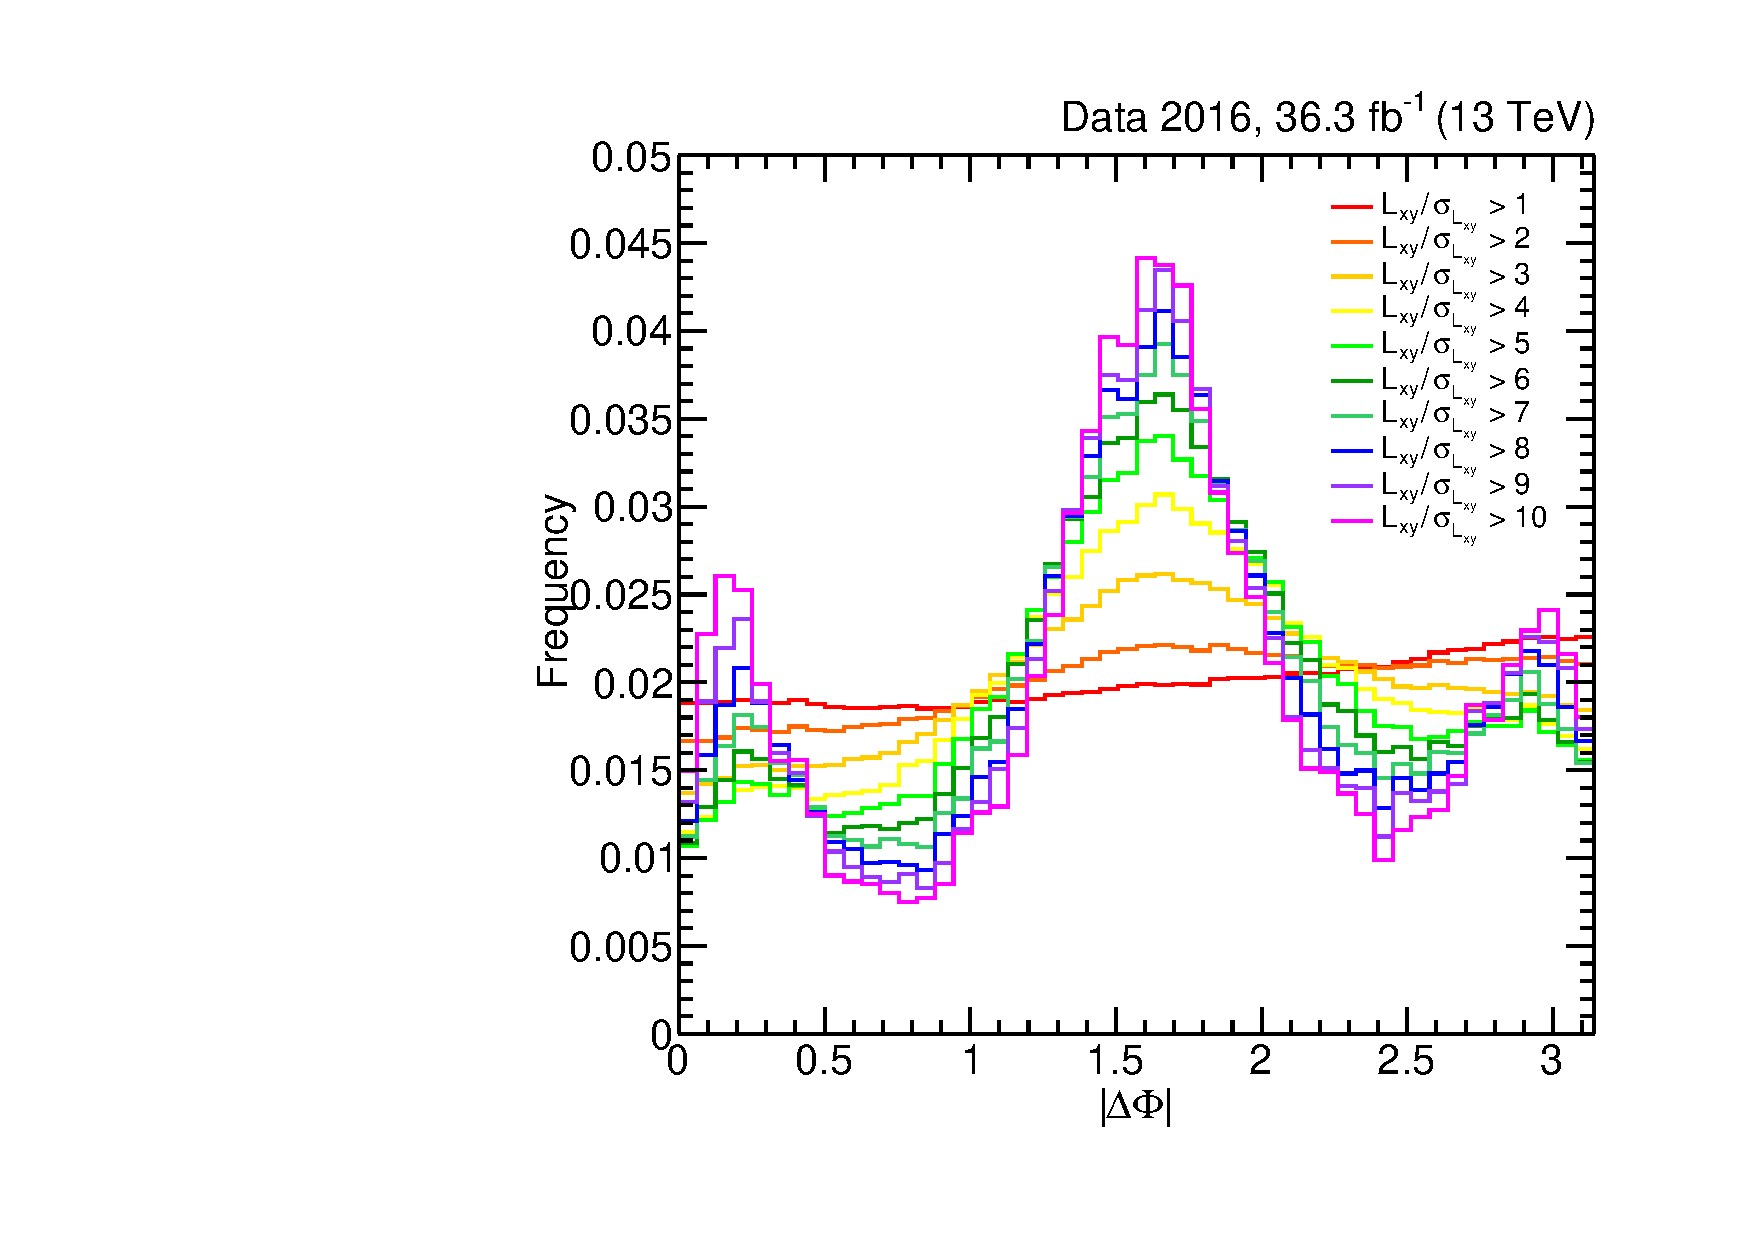
\includegraphics[width=\DSquareWidth]{figures/displaced/BGEST_EffectOfLxySigCut_DeltaPhi_Data_DY-Like.pdf}
  \hspace*{-2em}
  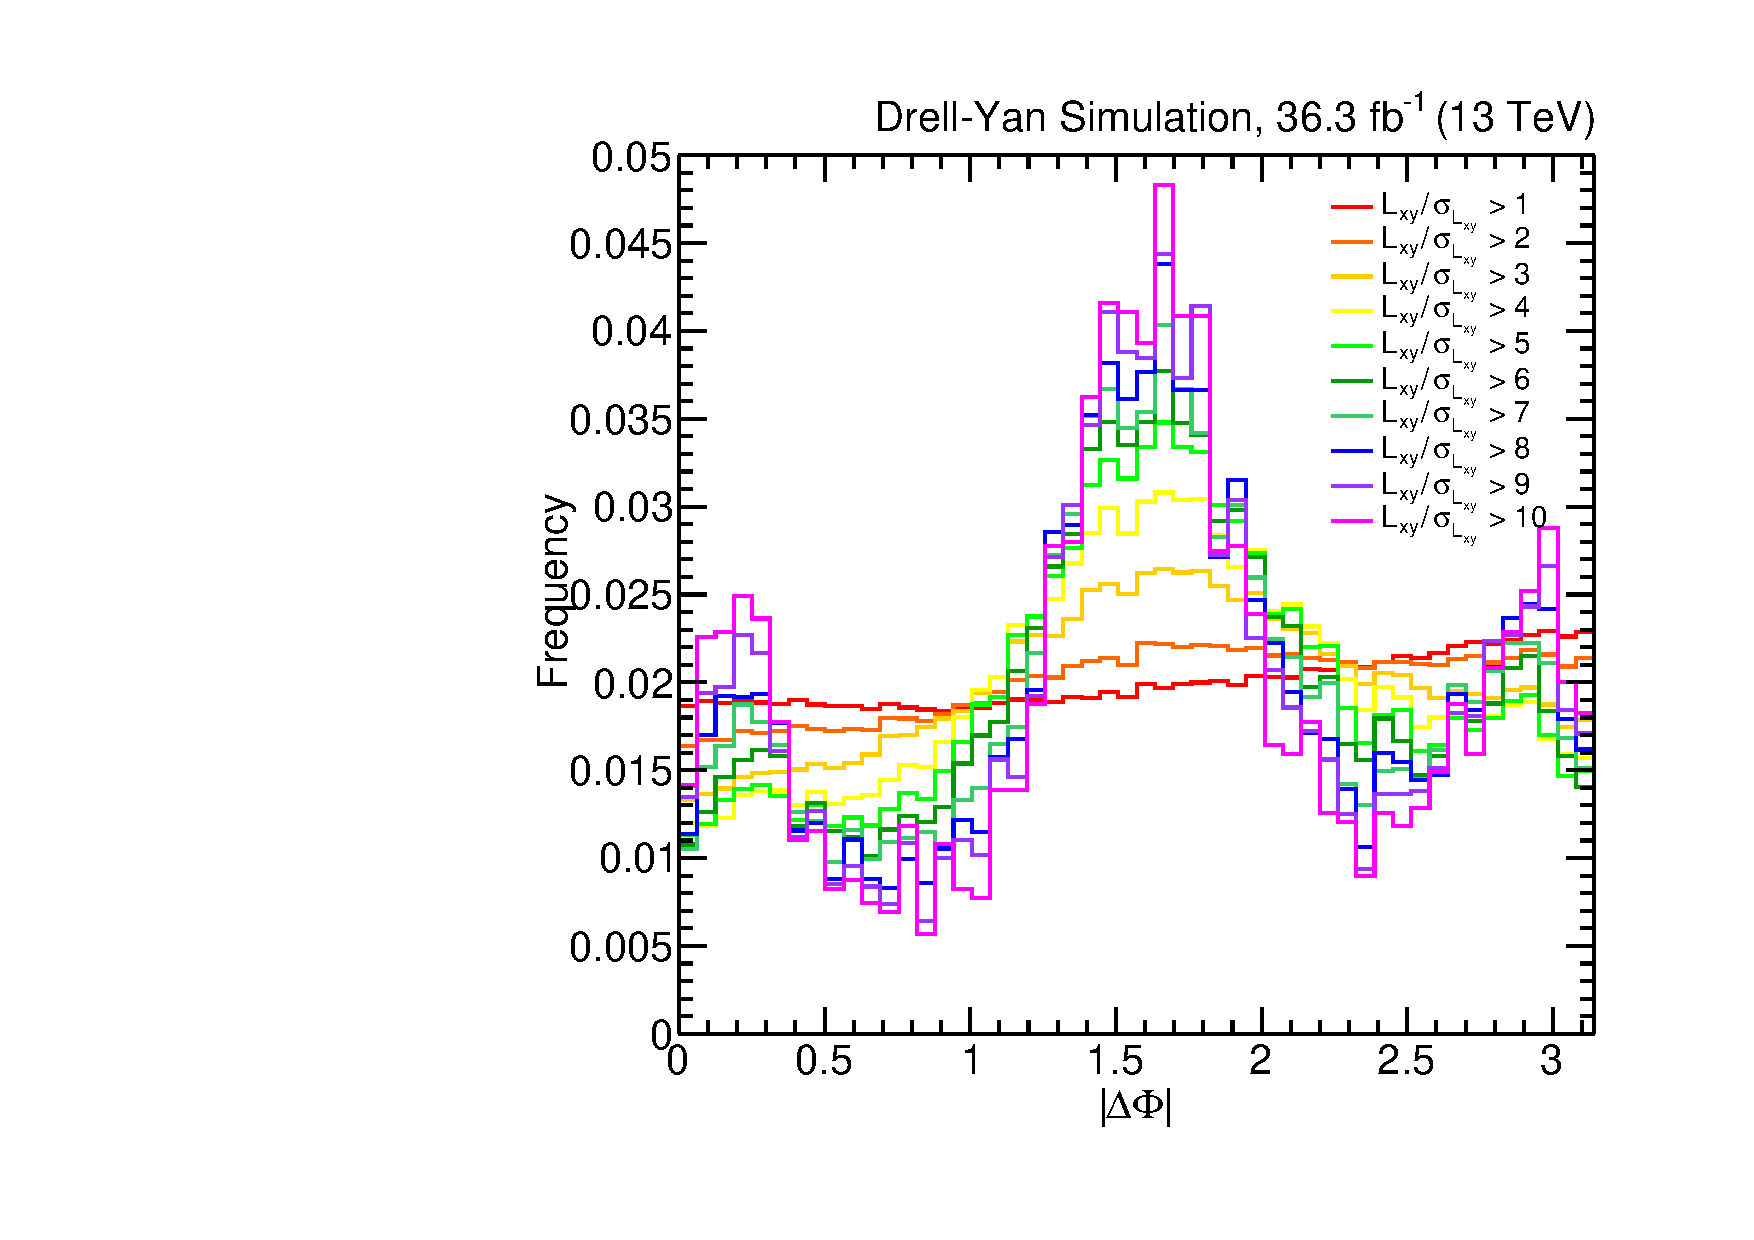
\includegraphics[width=\DSquareWidth]{figures/displaced/BGEST_EffectOfLxySigCut_DeltaPhi_MC_DY-Like.pdf}
  \caption[Histograms of \DeltaPhi for sequentially increasing cut values of \LxySig in data and Drell-Yan simulation.]{Histograms of \DeltaPhi as in \Fig~\ref{fig:dd:BGDeltaPhi_NoPAT}, normalized to unit area, for sequentially increasing cut values of \LxySig for \figpos{left} data and \figpos{right} Drell-Yan simulation.}
  \label{fig:dd:SeqLxySig}
\end{figure}

\begin{table}
  \centering
  \begin{tabular}{lcccl}
    \hline
    Name  & Events \\
    \hline
    SR                  & ?       \\
    \CR{\Full}{>6}{\pi} & 0       \\
    \CR{\Full}{<6}{0}   & 60      \\
    \CR{\Full}{<6}{\pi} & 55      \\
    \CR{D}    {>6}{0}   & 13636   \\
    \CR{D}    {>6}{\pi} & 17405   \\
    \CR{D}    {<6}{0}   & 1026522 \\
    \CR{D}    {<6}{\pi} & 1153133 \\
    \hline
  \end{tabular}
  \caption[Event counts for control regions for estimating Drell-Yan background.]{Event counts for control regions for estimating Drell-Yan background. The ratio of \CR{D}{>6}{\pi} to \CR{D}{>6}{0} gives a transfer factor; dividing the number of events in \CR{\Full}{>6}{\pi} by this transfer factor gives an estimate of the Drell-Yan background in SR.}
  \label{tab:dd:controlregions}
\end{table}

\Tab~\ref{tab:dd:controlregions} gives the number of events in data for each of the control regions.
A data-driven estimate of the transfer factor $\TF_\text{DY}$ can be obtained by dividing the number of events in \CR{D}{>6}{\pi} by the number of events in \CR{D}{>6}{0} and is found to be

\begin{equation}
  \TF_\text{DY} = \frac{N\left[\CR{D}    {>6}{\pi}\right]}{N\left[\CR{D}    {>6}{0}\right]} = 1.28
  \label{eq:dd:DYtransferfactor}
\end{equation}

Other ratios, such as $\CR{D}{<6}{\pi}/\CR{D}{<6}{0} = 1.12$ and $\CR{\Full}{<6}{\pi}/\CR{\Full}{<6}{0} = 0.92$ serve to validate the (approximate) symmetry in the Drell-Yan background (because the values are close to 1).

There are 0 events in the full 2016 dataset in \CR{\Full}{>6}{\pi}.
The estimate of the expected Drell-Yan background in SR is therefore also 0 events (with or without the mass window cuts described in \Sec~\ref{sec:dd:cutopt_mass}).
The systematic uncertainty on $\TF_\text{DY}$ is described and evaluated in \Sec~\ref{sec:dd:bgunc}.

\subsection{Estimation of QCD Background}
\label{sec:dd:bgest-QCD}
Background events arising from QCD processes, such as from collimated muons in jets, hadron decays in flight, or cascade decays of $b$ and $c$ quarks, may have large, signal-like \LxySig values and dimuon masses in the range $10\GeV < \mMuMu < 40\GeV$.
\DeltaPhi for such events may not be symmetric around $\pi/2$, instead having a peak at 0.

\Fig~\ref{fig:dd:SeqLxySig_QCD_DeltaPhi} illustrates this with a histogram of \DeltaPhi for opposite sign events with the \DSAToPAT association reversed, with the corresponding matched PAT dimuon satisfying $60 < \LxySig < 115$, and the constituent PAT muon tracks not isolated, for sequentially increasing cuts on DSA \LxySig.
Unlike the \mbox{Drell-Yan}-like events in the data plot of \Fig~\ref{fig:dd:SeqLxySig}, which are symmetric around $\pi/2$, these events have a strong, signal-like peak in \DeltaPhi at 0, especially for larger values of \LxySig.

\begin{figure}[htpb]
  \centering
  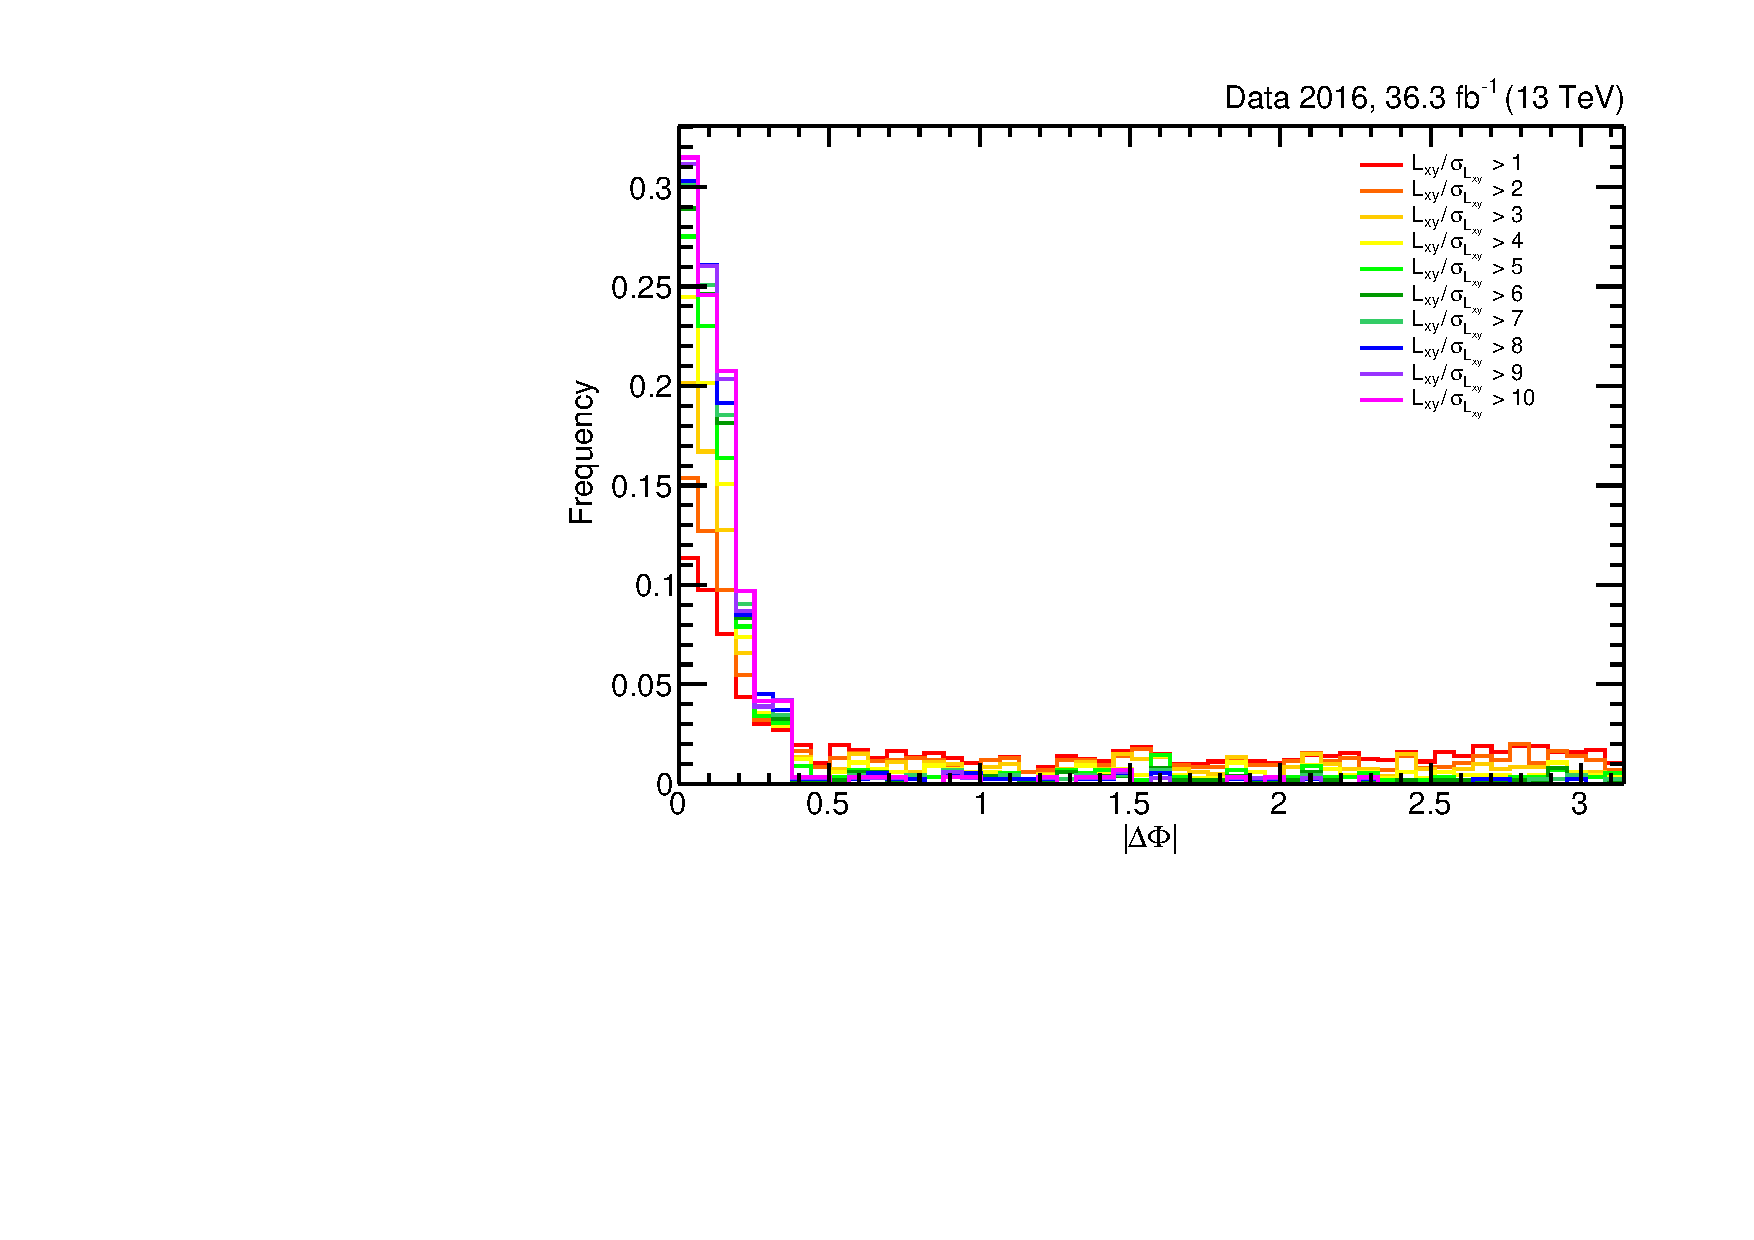
\includegraphics[width=\DFigWidth]{figures/displaced/BGEST_EffectOfLxySigCut_DeltaPhi_Data_QCD-Like.pdf}
  \caption[Histogram of \DeltaPhi for sequentially increasing cut values of \LxySig for QCD-like events in data.]{Histogram of \DeltaPhi for sequentially increasing cut values of \LxySig in data for the control region \CR[OS]{Q}{>x}{0}, normalized to unit area, with variable, sequentially increasing cut values $x$ of DSA \LxySig. These events are QCD-like, and have a strong, signal-like peak in \DeltaPhi at 0, especially for larger values of \LxySig, in stark contrast to the symmetry around $\pi/2$ of the \mbox{Drell-Yan}-like events in the data plot of \Fig~\ref{fig:dd:SeqLxySig}.}
  \label{fig:dd:SeqLxySig_QCD_DeltaPhi}
\end{figure}

\pagebreak
To demonstrate that calling these two sets of events \mbox{Drell-Yan}-like and QCD-like is justified, \Fig~\ref{fig:dd:SeqLxySig_DY_MassDeltaR} shows histograms of \mMuMu and $\deltaR(\Pgm\Pgm)$ for sequentially increasing cut values of \LxySig in data, as in \Fig~\ref{fig:dd:SeqLxySig}, for the events in the control region (\ie \CR{D}{>x}{0} for variable $x$) used to estimate the Drell-Yan background in \Sec~\ref{sec:dd:bgest-DY}.
As the cut increases, the contribution of the \PZ\ mass peak decreases, and the contribution of QCD events at lower mass increases slightly.
Moreover, the \deltaR distribution is highly \mbox{Drell-Yan}-like, with a strong peak at $\pi$ whose contribution also decreases with increasing \LxySig cut values, with some enhancement of low \deltaR QCD background.

In contrast, \Fig~\ref{fig:dd:SeqLxySig_QCD_MassDeltaR} shows similar histograms of \mMuMu and $\deltaR(\Pgm\Pgm)$ for the QCD-like events in data (\ie \CR[OS]{Q}{>x}{0} for variable $x$).
As the cut increases, the contribution of lower mass QCD events increases, and the \deltaR distribution has a strong peak at 0, suggestive of QCD background, with successively decreasing contributions from Drell-Yan backgrounds at $\pi$.

\begin{figure}[p]
  \centering
  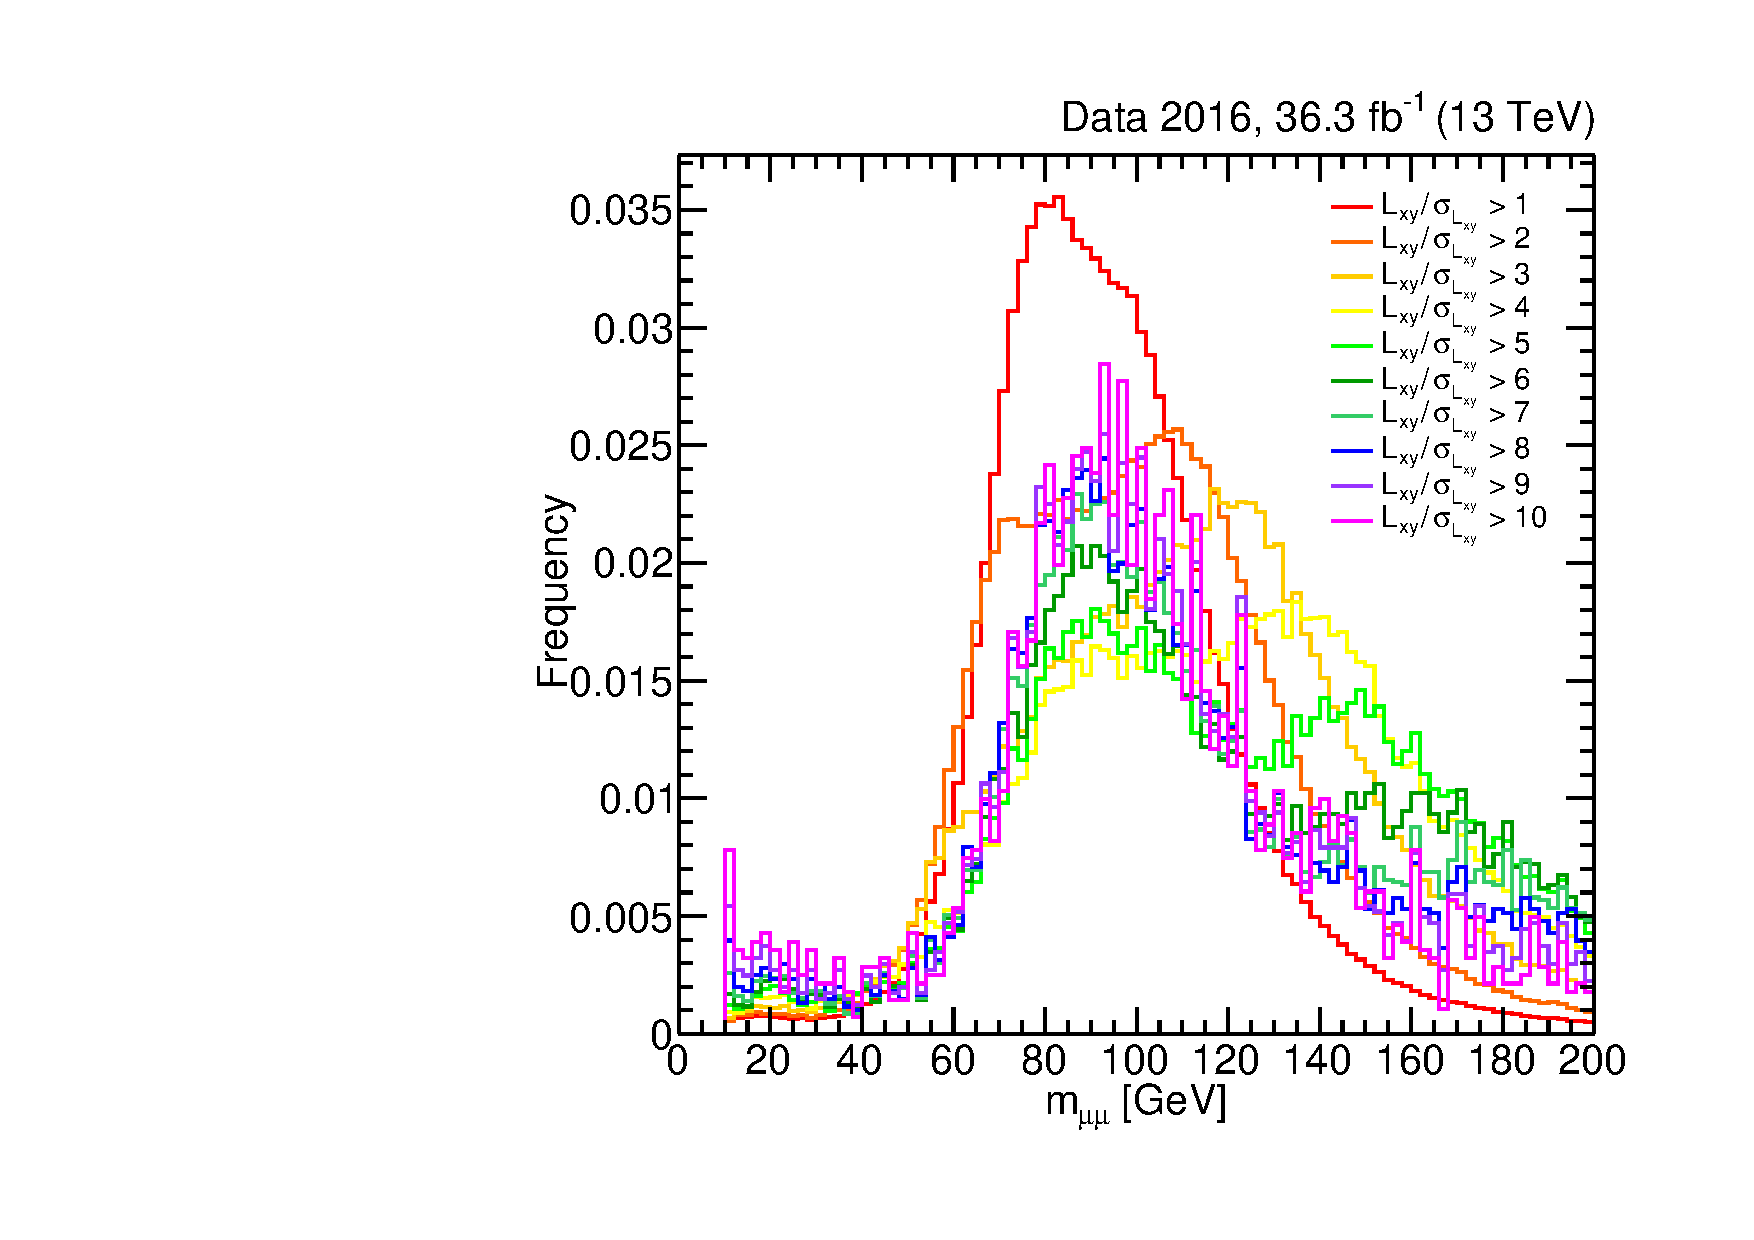
\includegraphics[width=\DSquareWidth]{figures/displaced/BGEST_EffectOfLxySigCut_Mass_Data_DY-Like.pdf}
  \hspace*{-2em}
  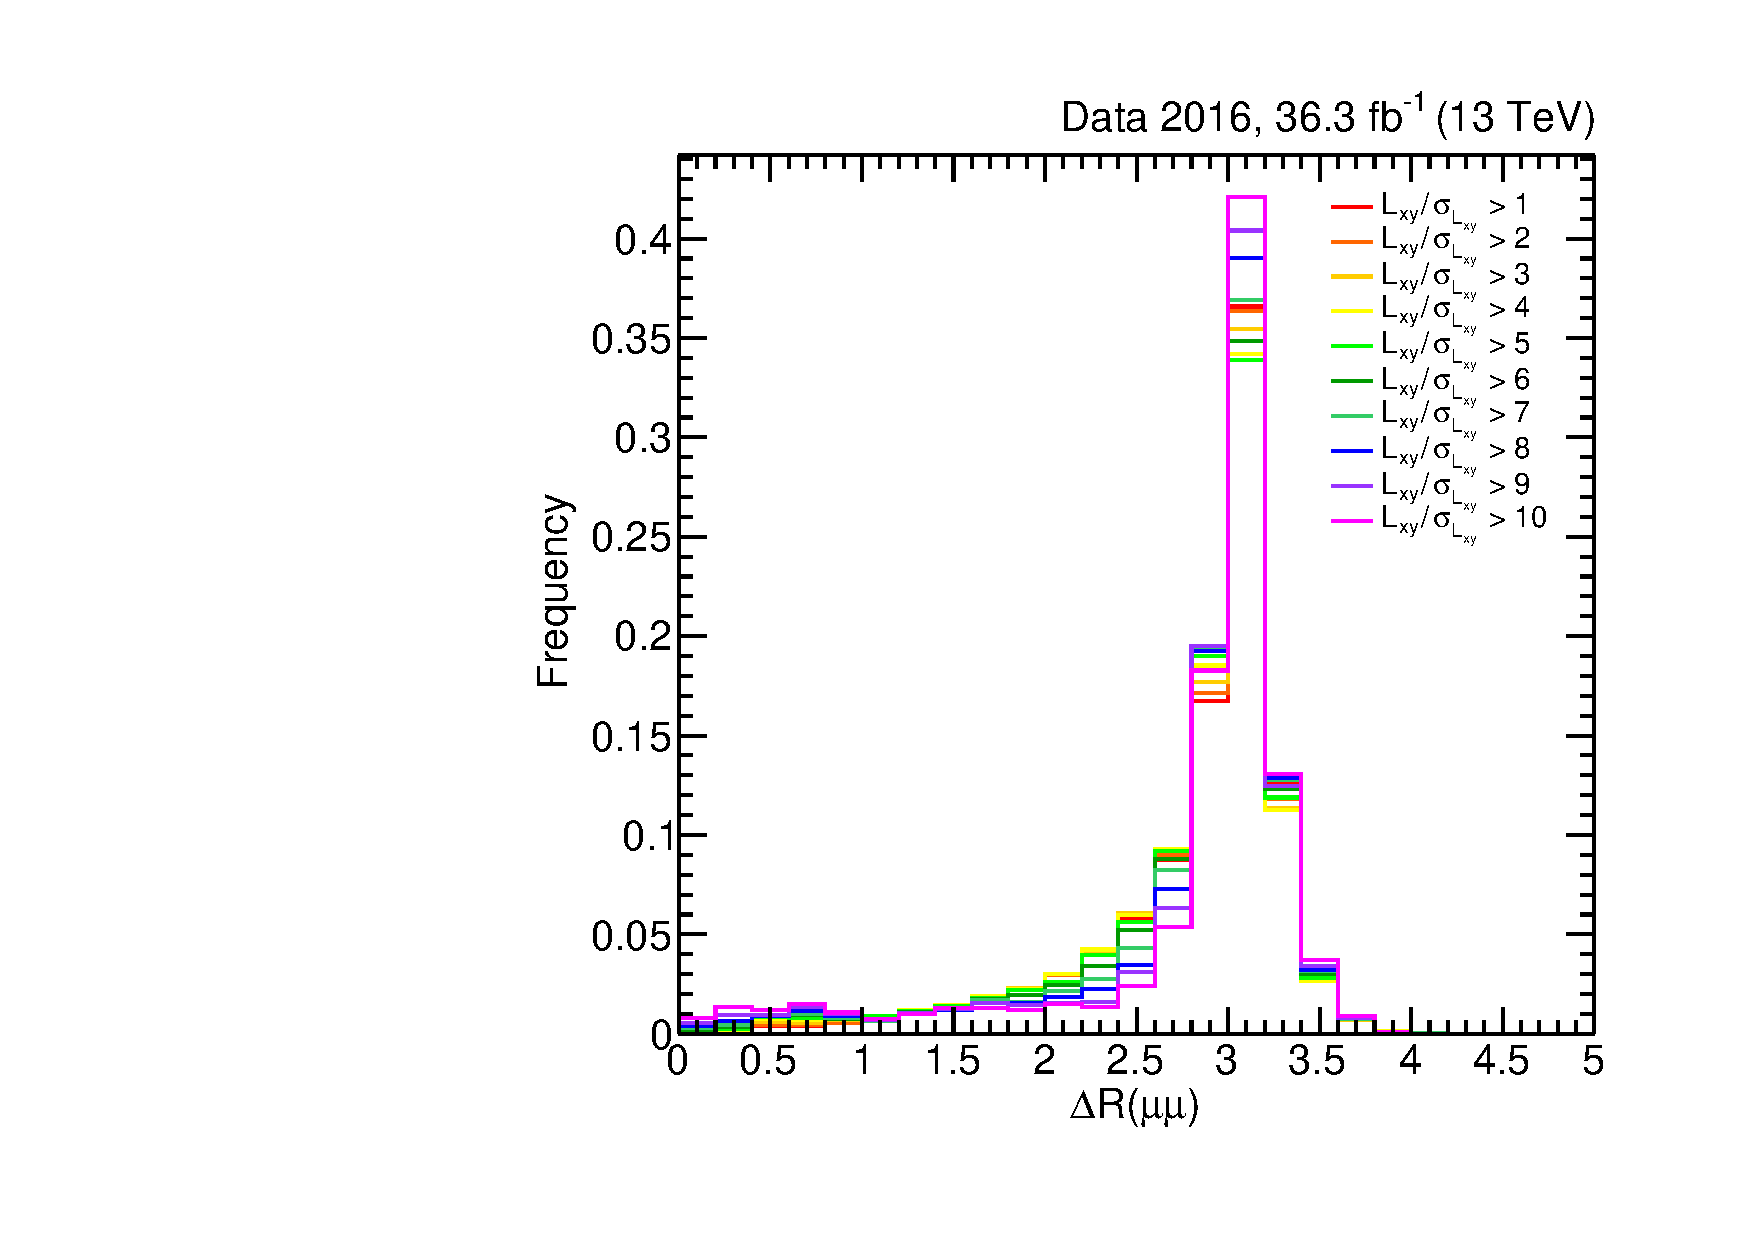
\includegraphics[width=\DSquareWidth]{figures/displaced/BGEST_EffectOfLxySigCut_DeltaR_Data_DY-Like.pdf}
  \caption[Histograms of \mMuMu and $\deltaR(\Pgm\Pgm)$ for \mbox{Drell-Yan}-like events in data for sequentially increasing cut values of \LxySig.]{Histograms of \figpos{left} \mMuMu and \figpos{right} $\deltaR(\Pgm\Pgm)$ for sequentially increasing cut values of \LxySig in data as in \Fig~\ref{fig:dd:SeqLxySig}, normalized to unit area, using the control regions \CR{D}{>x}{0} for variable, sequentially increasing cut values $x$ of DSA \LxySig.}
  \label{fig:dd:SeqLxySig_DY_MassDeltaR}
\end{figure}

\begin{figure}[p]
  \centering
  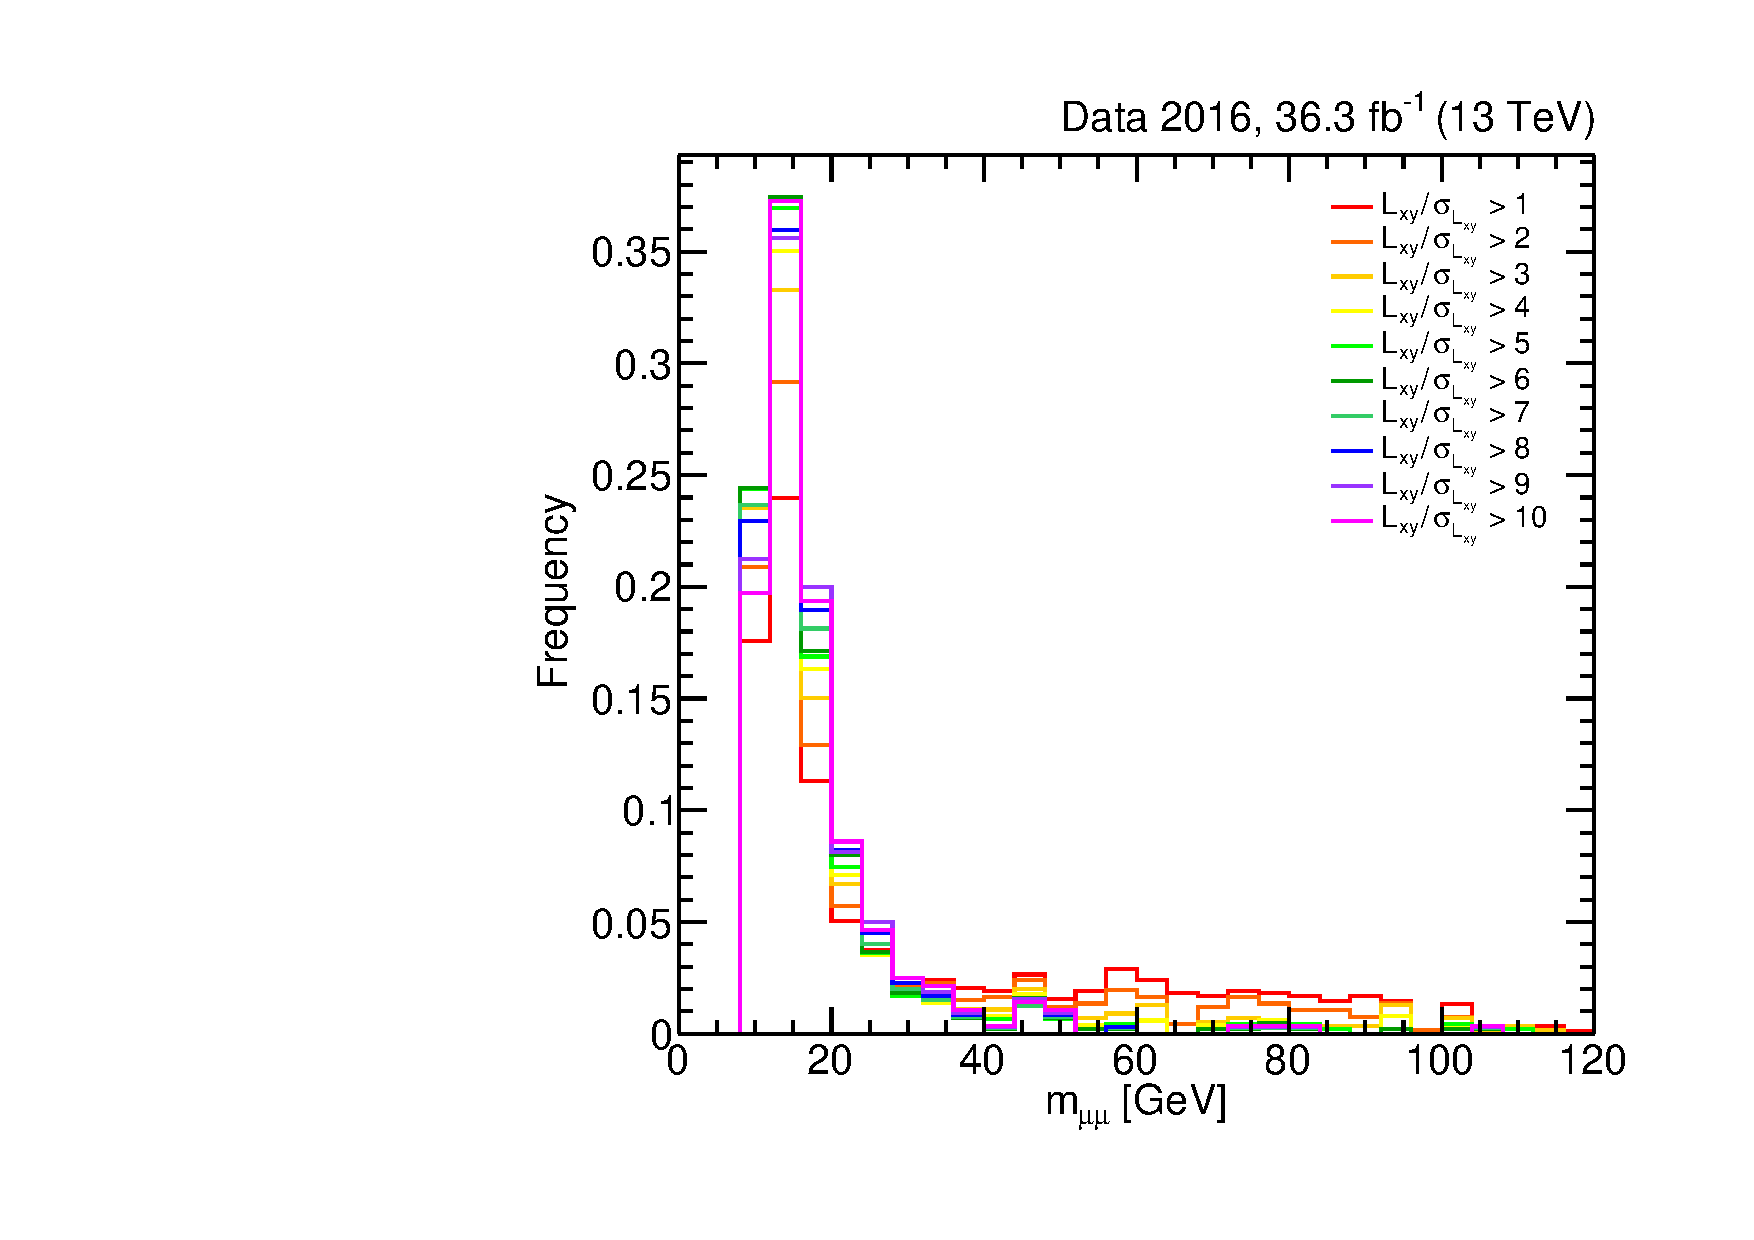
\includegraphics[width=\DSquareWidth]{figures/displaced/BGEST_EffectOfLxySigCut_Mass_Data_QCD-Like.pdf}
  \hspace*{-2em}
  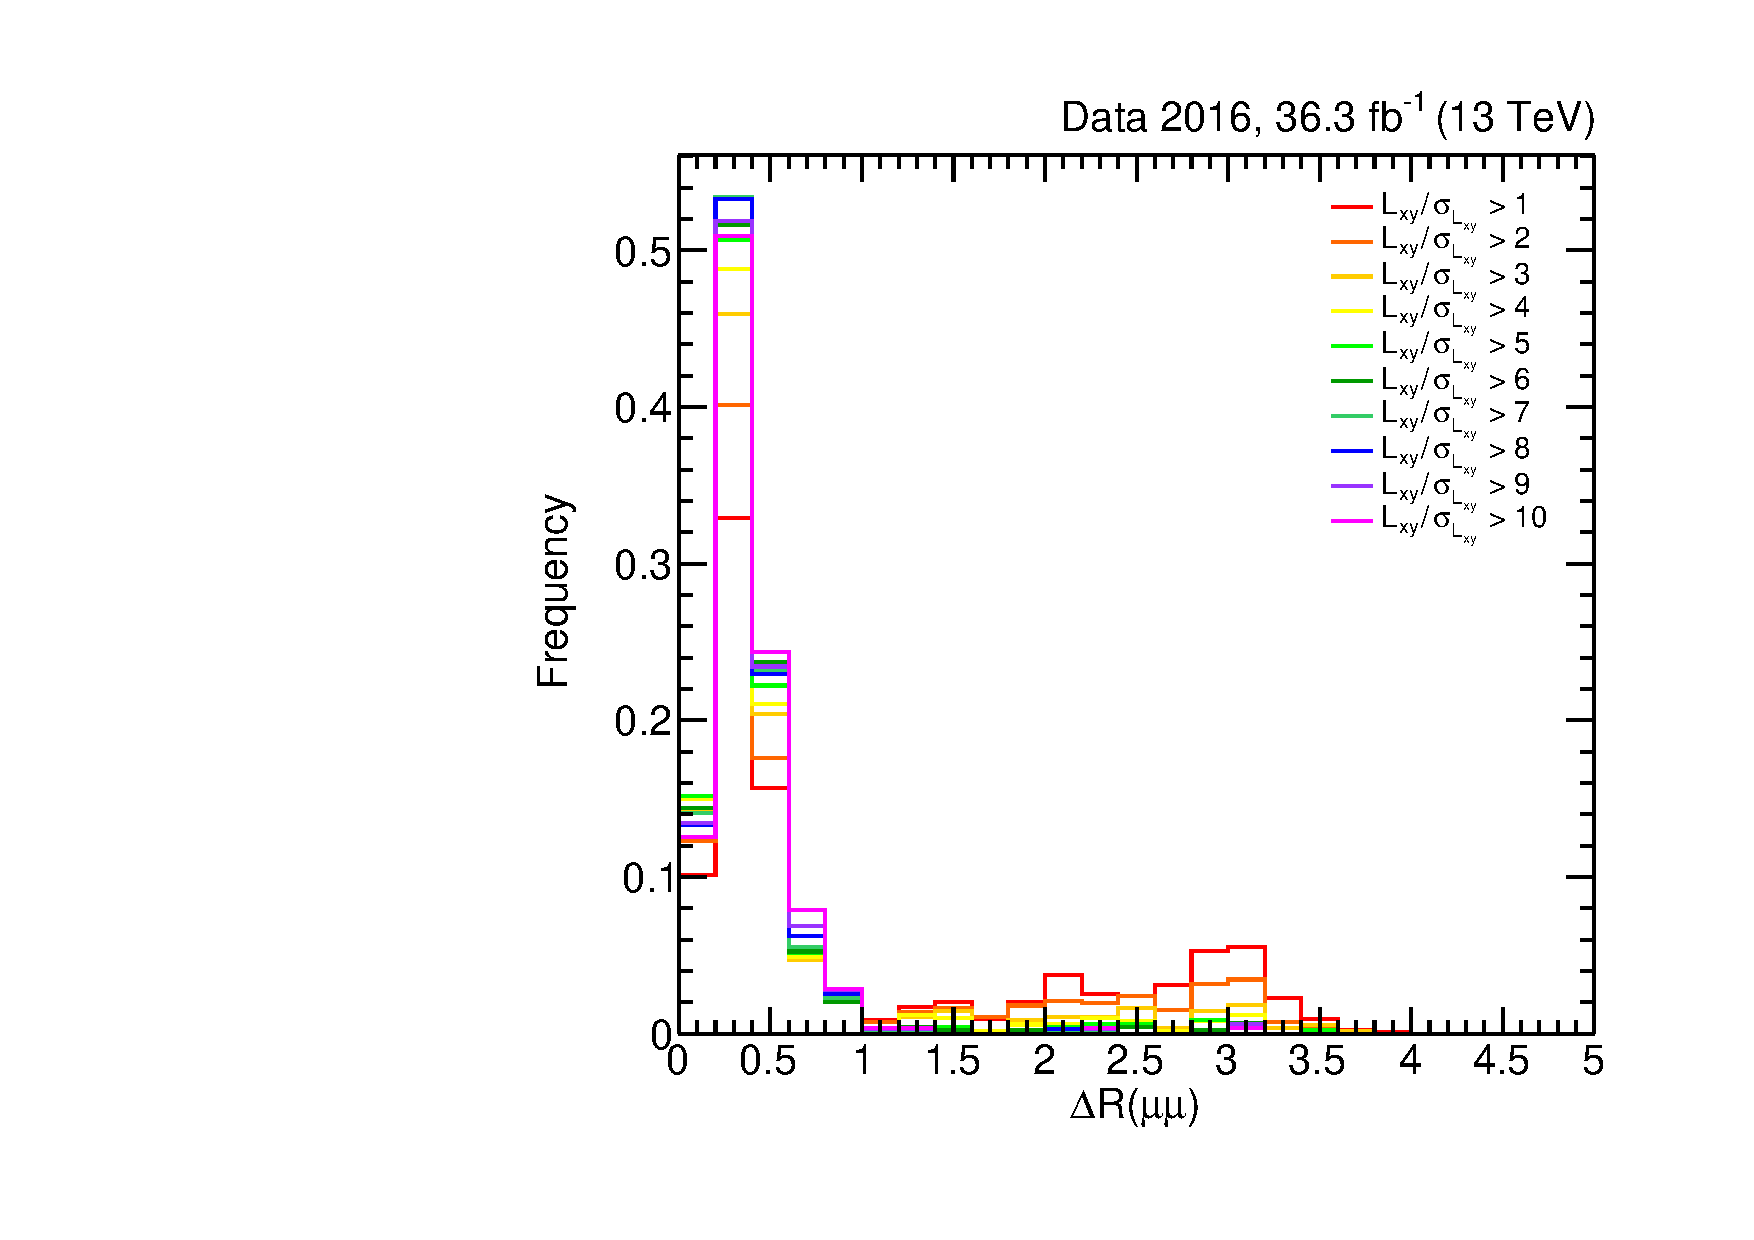
\includegraphics[width=\DSquareWidth]{figures/displaced/BGEST_EffectOfLxySigCut_DeltaR_Data_QCD-Like.pdf}
  \caption[Histograms of \mMuMu and $\deltaR(\Pgm\Pgm)$ for QCD-like events in data for sequentially increasing cut values of \LxySig.]{Histograms of \figpos{left} \mMuMu and \figpos{right} $\deltaR(\Pgm\Pgm)$ as in \Fig~\ref{fig:dd:SeqLxySig_DY_MassDeltaR}, but for QCD-like events in data, using the control regions \CR{Q}{>x}{0} for variable, sequentially increasing cut values $x$ of DSA \LxySig.}
  \label{fig:dd:SeqLxySig_QCD_MassDeltaR}
\end{figure}

Such QCD-like events hence would not appear in control regions with low \LxySig or high \DeltaPhi, and estimation of this background cannot be performed with a transfer factor applied to events in \CR{\Full}{>6}{\pi}.

Instead, pairs of regions with same-sign dimuons and opposite-sign dimuons are considered.
\Tab~\ref{tab:dd:QCDcontrolregions} gives the number of events in data for several control regions.
The relevant control regions are then \CR[OS]{Q}{>6}{0} and \CR[SS]{Q}{>6}{0}, and the transfer factor obtained thus can be applied to \CR[SS]{\Full}{>6}{0} to obtain a QCD background estimate for \CR[OS]{\Full}{>6}{0}.
This transfer factor has a value of
\begin{equation}
  \TF_\text{QCD} = \frac{N\left[\CR[OS]{Q}{>6}{0}\right]}{N\left[\CR[SS]{Q}{>6}{0}\right]} = 2.81
  \label{eq:dd:QCDtransferfactor}
\end{equation}

There are 4 same-sign events in \CR[SS]{Q}{>6}{0} in the full 2016 dataset, giving an estimate of QCD background in the SR of 11.2 events (without the mass window cuts described in \Sec~\ref{sec:dd:cutopt_mass}).
As with the Drell-Yan transfer factor, there is a large systematic uncertainty on the QCD transfer factor (among other factors, it is sensitive to the window used for the PAT \LxySig); this uncertainty will be described and evaluated in \Sec~\ref{sec:dd:bgunc}.

\begin{table}
  \centering
  \begin{tabular}{lcccl}
    \hline
    Name  & Events \\
    \hline
    SR                    & ?   \\
    \CR[SS]{\Full}{>6}{0} & 4   \\
    \CR[OS]{\Full}{<6}{0} & 60  \\
    \CR[SS]{\Full}{<6}{0} & 4   \\
    \CR[OS]{Q}  {>6}{0}   & 323 \\
    \CR[SS]{Q}  {>6}{0}   & 115 \\
    \CR[OS]{Q}  {<6}{0}   & 314 \\
    \CR[SS]{Q}  {<6}{0}   & 196 \\
    \hline
  \end{tabular}
  \caption[Event counts for control regions for estimating QCD background.]{Event counts for control regions for estimating QCD background. A ratio of events in \CR[SS]{Q}{>6}{0} with same-sign muons to the corresponding control region with opposite-sign muons \CR[OS]{Q}{>6}{0} gives a transfer factor; multiplying the number of events in \CR[SS]{\Full}{>6}{0} by this transfer factor gives an estimate of the QCD background in SR.}
  \label{tab:dd:QCDcontrolregions}
\end{table}

Other ratios in \Tab~\ref{tab:dd:controlregions} do not give an appropriate transfer factor but rather serve to illuminate features of the QCD background.
The ratio of \CR[OS]{Q}{<6}{0} to \CR[SS]{Q}{<6}{0} is 1.6, much closer to 1; this clarifies that there is proportionally more opposite-sign QCD background for large values of \LxySig, and so a large \LxySig region needed to be used to quantify it.
The ratio of \CR[SS]{\Full}{<6}{0} to \CR[OS]{\Full}{<6}{0} is quite small, showing that the same-sign background is not an important contributor to the regions with small \LxySig, and so the same-sign events in this region could not have been used to extrapolate an estimate in the signal region.

\section{Cut Optimization}
This section describes a few procedures applied to fine-tune the event and object selection to optimize the analysis for the statistical significance of a potential signal discovery.

\subsection[Optimizing with \ZBi as a Figure of Merit]{Optimizing with \texorpdfstring{$\bm{Z_{\mathbf{Bi}}}$}{ZBi} as a Figure of Merit}
\label{sec:dd:cutopt_ZBi}
As a set of analysis selections varies, the numbers of signal and background events also vary, and so fine-tuning the values of cuts is an exercise in balancing signal efficiency \vs background rejection.
The metric for determining an optimal cut value, as a function of the number of signal and background events, is a figure of merit that is monotonic with the expected statistical significance of a discovery.
The figure of merit used in this analysis is \ZBi \cite{Cousins:ZBi2008}, an estimate of the statistical significance of an excess number of events in a signal region when the number of background events is estimated from a control region.
The subscript is an abbreviation for \textbf{Bi}nomial, because under the background-only hypothesis, the splitting of events between the signal and control region follows a binomial distribution with binomial parameter equal to the expected fraction of background in the signal region out of the background in both regions.
In the notation introduced in \Sec~\ref{sec:dd:bgest}, with \TF the transfer factor, this binomial parameter is $1/(1+\TF)$.

A procedure based on \ZBi as a figure of merit was performed on several key discriminating variables.
The following description of the procedure will be phrased in terms of optimizing the \LxySig cut.
A background distribution of \LxySig is defined as a histogram of data events in the (approximately) signal-free region $\DeltaPhi > \pi/2$, and a corresponding signal distribution of \LxySig is defined as a histogram of signal events in the signal region \mbox{$\DeltaPhi < \pi/2$}, with both distributions consisting of events passing all selections except for the \LxySig cut.
The signal histogram is scaled to 2016 integrated luminosity assuming an arbitrary production cross section of $1\times 10^{-2}\unit{pb}$.
For \LxySig, the number of events in either histogram passing a given cut is an integral from the cut value to infinity; for some other variables (such as track \normchisq), the number of events passing a given cut is an integral from zero to the cut value.
In the following discussion, the ``integral'' of a histogram is assumed to be performed over the appropriate interval.

In the notation found in Reference~\cite{Cousins:ZBi2008}, the integral of the simulated signal histogram corresponds to an estimate $\hat{\mu}_s$ of the true Poisson mean number of signal events in the signal region;
and the integral of the background histogram corresponds to a number of observed events in the signal-free region $n_\text{off}$, from which one derives the estimate $\hat{\mu}_b = n_\text{off}/\TF$ of the true Poisson mean number of background events in the signal region.
\ZBi is then calculated for each cut value, a function of three quantities: the number of background events in the control region $n_\text{off}$, the total number of observed events in the signal region $n_\text{on} = \hat{\mu}_s + \hat{\mu}_b$, and the transfer factor is taken to be $\TF = 1$.

\Fig~\ref{fig:dd:CutOptExample} shows an example of the cut optimization procedure, with the background (control region in data) distribution in red, the signal distribution (here for the \twoMu signal sample with \FullSP{1000}{20}{20}) in blue, and the value of \ZBi for each cut value in green.
The tail of the signal distribution is much longer than in the background distribution, which peaks strongly at smaller values of \LxySig, so \ZBi rises steadily until about 5 or 6.
For this signal sample, the cut value of \LxySig corresponding to the largest value of \ZBi is between 6 and 7.

\begin{figure}[htpb]
  \centering
  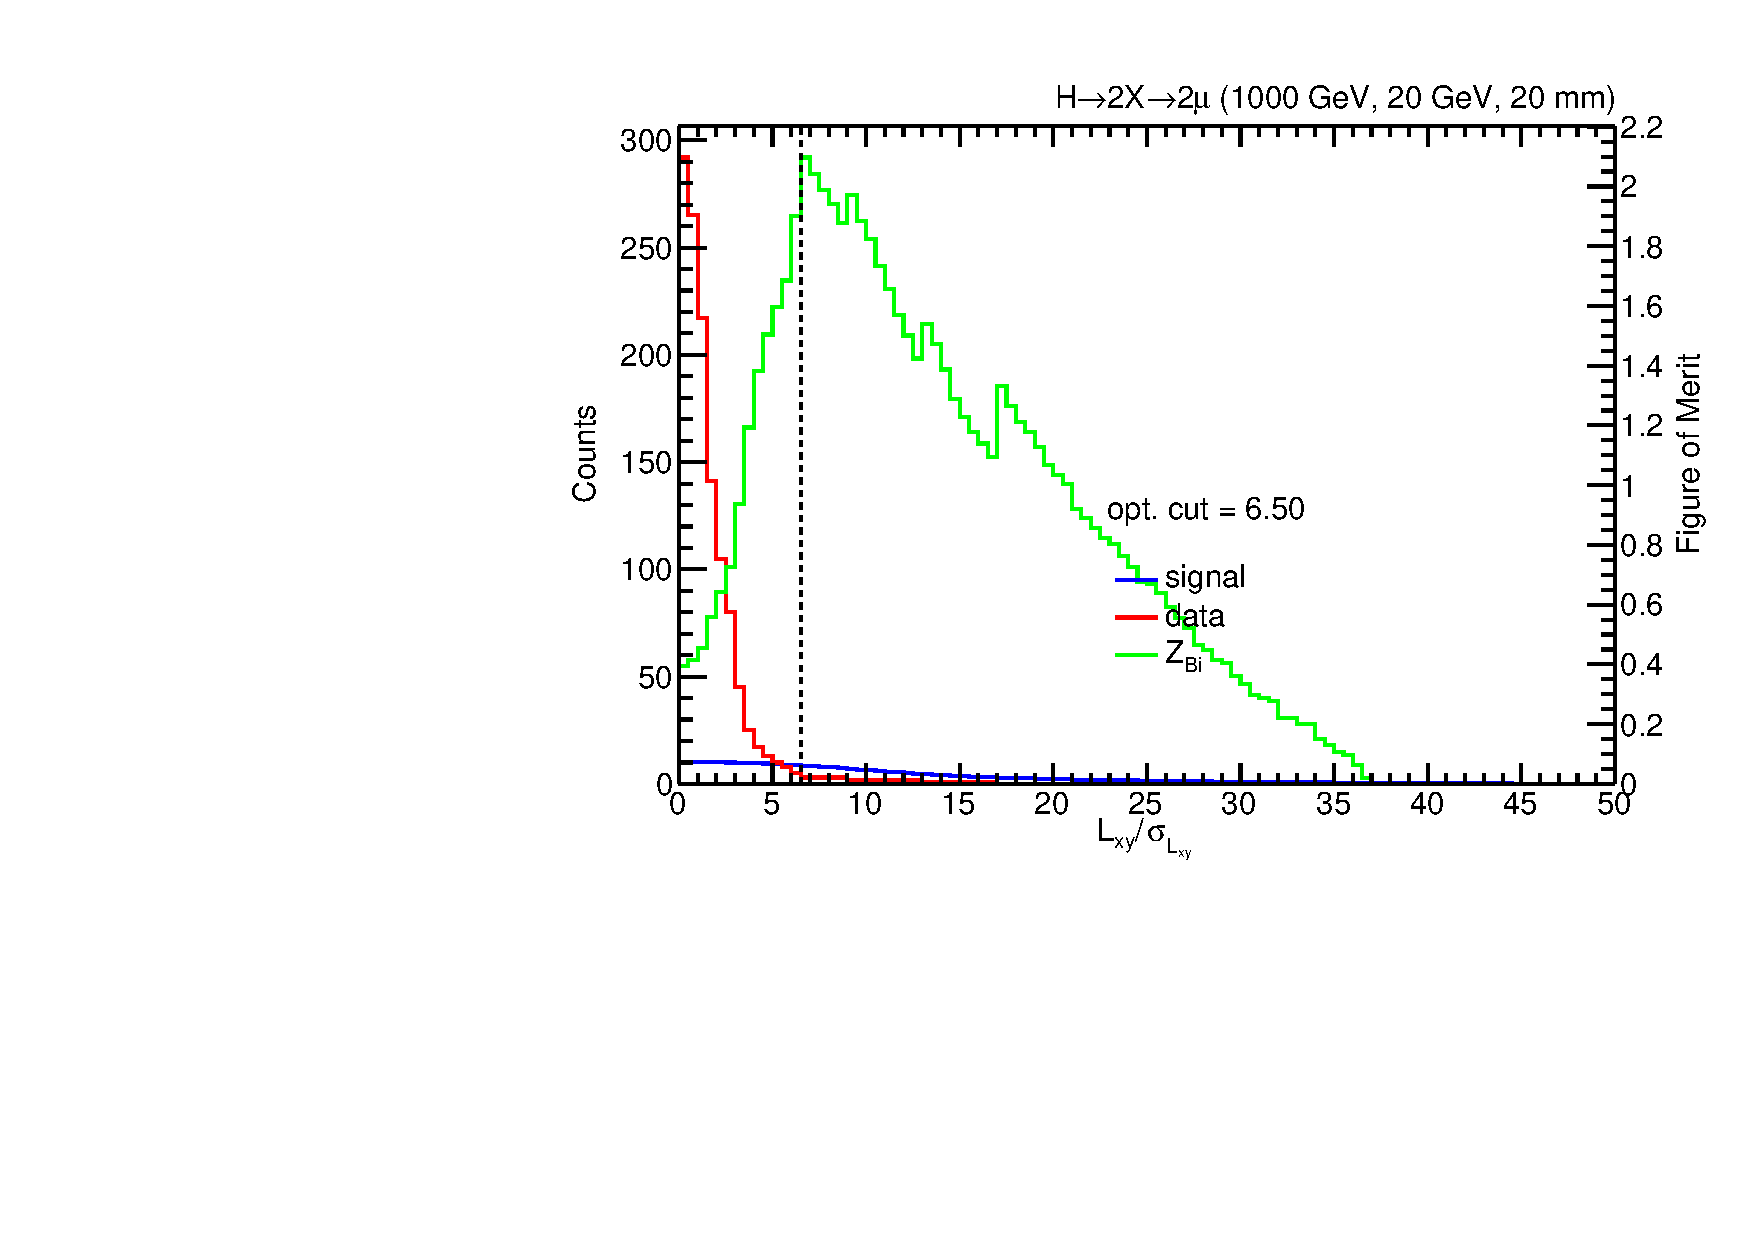
\includegraphics[width=\DFigWidth]{figures/displaced/OPT_LxySig_ZBi_HTo2XTo2Mu2J_1000_20_20.pdf}
  \caption[Example of \ZBi-based cut optimization of \LxySig.]{Example of \ZBi-based cut optimization of \LxySig for the \twoMu signal sample with \FullSP{1000}{20}{20}. The background distribution is in red and corresponds to a selection of events in a control region of data; the signal distribution is in blue; and the value of \ZBi at each cut value is in green. Here, the cut value of \LxySig corresponding to the largest value of \ZBi is between 6 and 7, marked on the plot as 6.5. As a consequence of the background distribution having a strong peak at small values of \LxySig and the tail in the signal distribution being much longer, the \ZBi curve rises steadily for tighter cuts on \LxySig, peaks, and then falls.}
  \label{fig:dd:CutOptExample}
\end{figure}

This procedure was performed on all signal samples, with a systematic grid of cut values in several variables.
The main results of this \ZBi-based cut optimization are:
\begin{itemize}
  \item \ZBi rises steadily as cuts on \LxySig and track \normchisq are tightened, informing the choices of cut values of 6 and 2.5, respectively. Although for some sets of selections, \ZBi continues to increase for tighter cuts, the shape flattens out considerably after these thresholds, so the increases in \ZBi are minimal, and the shape becomes highly sensitive to the specific background events and the specific numbers of events used to tune the cuts. The choices of cut values take these effects into account.
  \item \ZBi does not increase appreciably for any requirement on the muon track impact parameter significance ($d_0/\sigma_{d_{0}}$) once a requirement on \LxySig requirement is in place, so the analysis selection does not impose any cuts on $d_0/\sigma_{d_{0}}$. This was a requirement that was used in previous versions of this analysis performed with Run 1 data \cite{EXO-12-037,CMS-PAS-EXO-14-012}. Similarly, no appreciable increase in \ZBi was observed for tighter cuts on vertex \chisq than 20 once other cuts are in place.
\end{itemize}

\subsection{Dimuon Mass Window Selection}
\label{sec:dd:cutopt_mass}
When computing upper limits on long-lived particle production cross sections, it is undesirable to include in the observation dimuon events with invariant masses appreciably different from the invariant mass postulated by the signal model under consideration.
To implement this requirement, the reconstructed dimuon invariant mass histograms (for each value of generated long-lived particle mass \mX, for events passing the full selection in \twoMu signal) are fit to Gaussian distributions, yielding a mean and standard deviation, $\mu_{\mX}$ and $\sigma_{\mX}$.
\Fig~\ref{fig:dd:massdistributions} shows the distributions of reconstructed dimuon mass for \twoMu signal samples, combining all sets of signal parameters for each value of \mX, for events passing all selections except for the mass cut, along with a fitted Gaussian for each distribution.
The dimuon invariant mass is required to lie within a mass window given by $\mu_{\mX} \pm 3\sigma_{\mX}$, with the lower limit at least 10\GeV and no upper limit for the largest generated mass.
This selection is more than 99\% efficient in most \twoMu signal samples (97\% in the worst case).
\Tab~\ref{tab:dd:masswindow} enumerates the invariant mass window selection (applied to reconstructed dimuons) used for each generated value of \mX.

\begin{figure}[htbp]
  \centering
  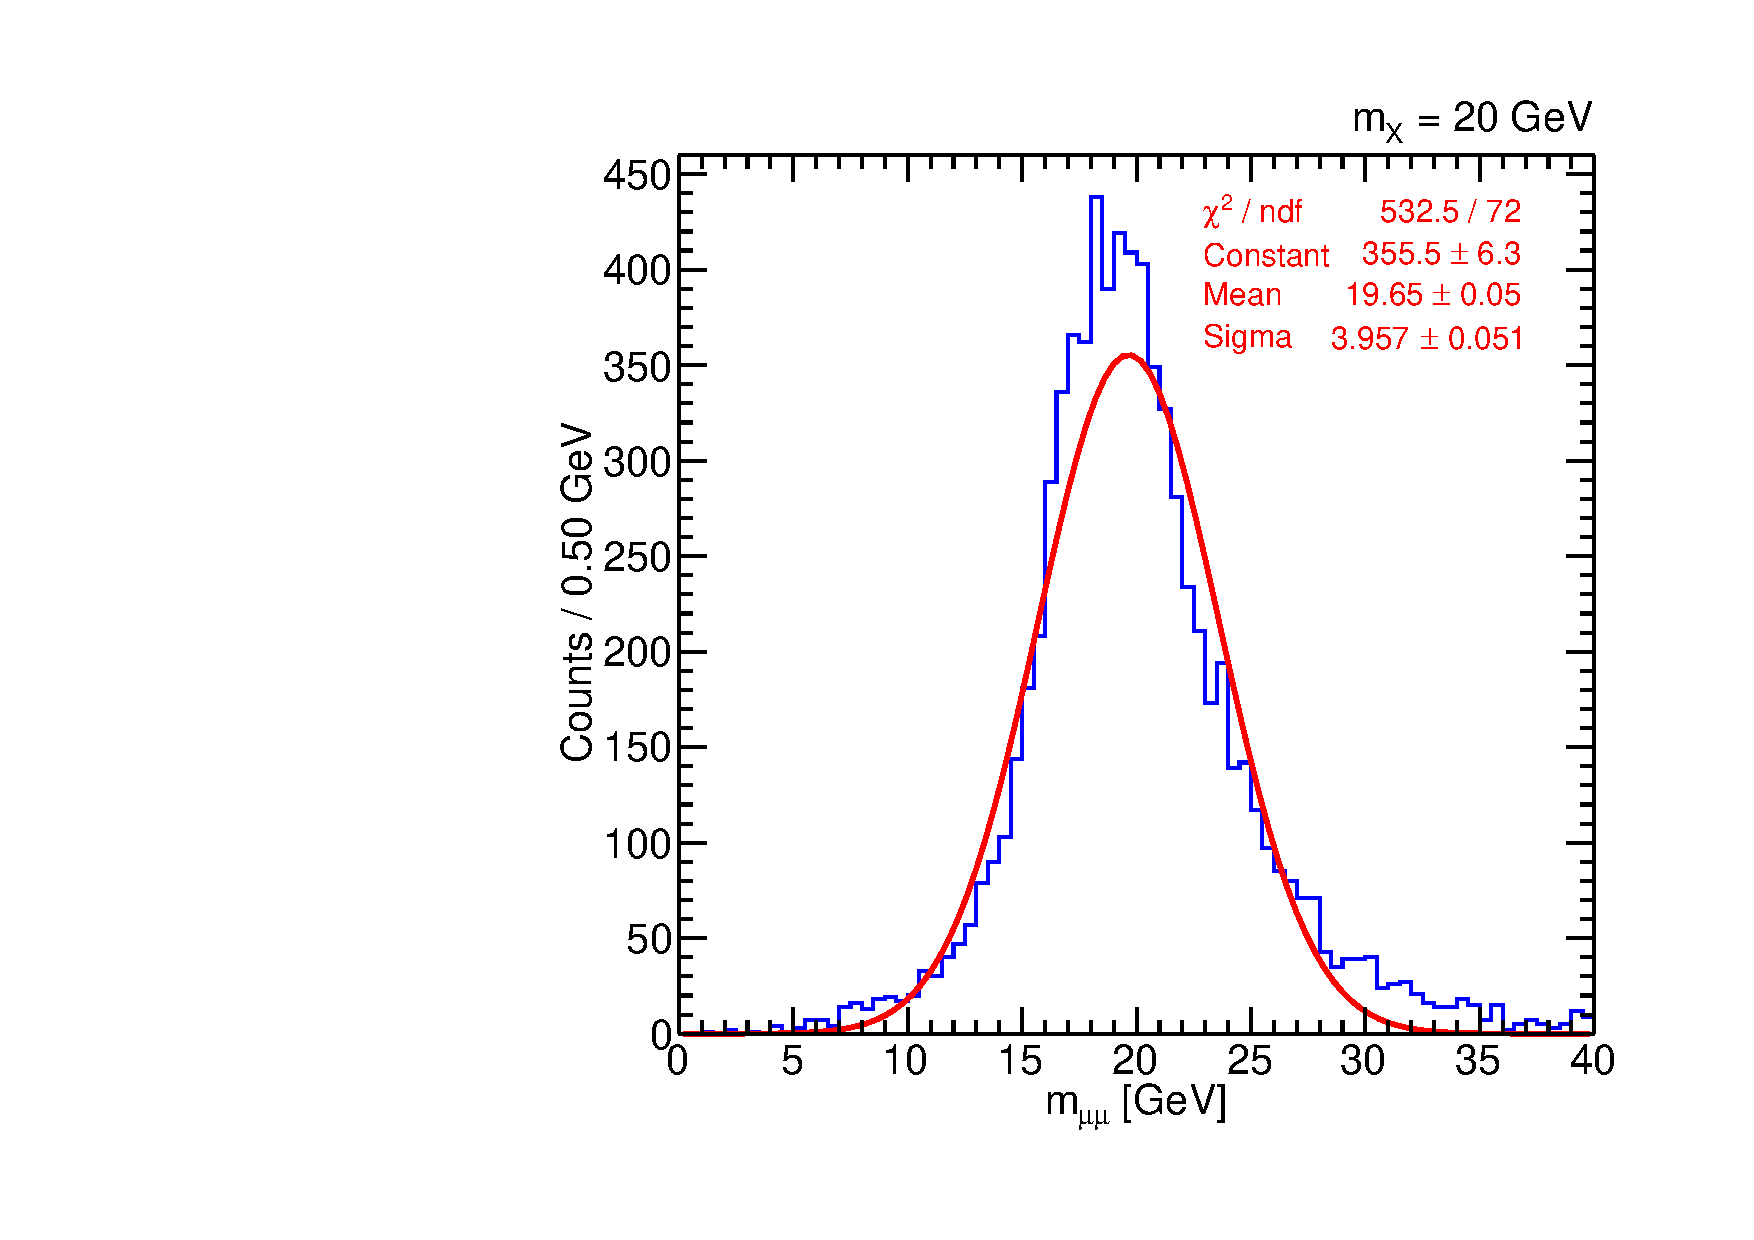
\includegraphics[width=\DSquareWidth]{figures/displaced/MASS_2Mu2J_20.pdf}
  \hspace*{-2em}
  \includegraphics[width=\DSquareWidth]{figures/displaced/MASS_2Mu2J_50.pdf} \\
  \includegraphics[width=\DSquareWidth]{figures/displaced/MASS_2Mu2J_150.pdf}
  \hspace*{-2em}
  \includegraphics[width=\DSquareWidth]{figures/displaced/MASS_2Mu2J_350.pdf}
  \caption[Reconstructed invariant dimuon mass distributions for \twoMu signal samples, long with fitted Gaussian curves for each distribution.]{Reconstructed invariant dimuon mass distributions for \twoMu signal samples passing all selections except the mass cut, combining all sets of signal parameters for each value of \mX, along with fitted Gaussian curves for each distribution.}
  \label{fig:dd:massdistributions}
\end{figure}

\begin{table}
  \centering
  \begin{tabular}{rrrl}
    \hline
    Generated \mX & \multicolumn{1}{c}{$\mu$} & \multicolumn{1}{c}{$\sigma$} & Dimuon Mass Window           \\
    \hline
     20\GeV       &  20\GeV &   4\GeV & $10\GeV < \mMuMu < 32\GeV$   \\
     50\GeV       &  50\GeV &  10\GeV & $20\GeV < \mMuMu < 80\GeV$   \\
    150\GeV       & 140\GeV &  35\GeV & $35\GeV < \mMuMu < 245\GeV$  \\
    350\GeV       & 320\GeV &  85\GeV & $65\GeV < \mMuMu$            \\
    \hline
  \end{tabular}
  \caption[Dimuon invariant mass window selections for each value of generated long-lived particle mass \mX.]{Dimuon invariant mass window selections for each value of generated long-lived particle mass \mX, along with values for the fitted Gaussian $\mu$ and $\sigma$. The windows are defined as $\mu \pm 3\sigma$ with the lower limit at least 10\GeV and no upper limit for the largest generated mass.}
  \label{tab:dd:masswindow}
\end{table}

\subsection{N--1 Plots}
This section presents selected ``N$-$1'' plots, so named because they are histograms of events passing the full selection except for one cut: the variable plotted.
Such plots depict the events that passed all other cuts and would be removed by applying the cut in question, and so convey the effect of individual cuts in the analysis.
These plots also provide a structured way of comparing the distributions and the fraction of events passing each cut in signal and background.
The analysis selections should be highly efficient in signal and highly inefficient in background.

\Figs~\ref{fig:dd:NM1_pT}--\ref{fig:dd:NM1_LxySig} are the N$-$1 plots for selected variables, for events in all \twoMu signal samples combined and for events in the control region \CR{\Full}{>6}{\pi} of data.
The cut values are labeled on the plots, as is the efficiency of the selection.
The cosmic rejection cuts on $\cos{\alpha}$ and number of parallel pairs are highly correlated, and so the corresponding plots, \Fig~\ref{fig:dd:NM1_cosAlpha} and \Fig~\ref{fig:dd:NM1_Npp}, omit both cuts from both sets of plots; for this reason they are actually ``N$-$2'' plots.

\begin{figure}[p]
  \centering
  \includegraphics[width=\DSquareWidth]{figures/displaced/NM1_2Mu2J_pT.pdf}
  \hspace*{-2em}
  \includegraphics[width=\DSquareWidth]{figures/displaced/NM1_Data_pT.pdf}
  \caption[Histograms of events passing the full selection except for the muon \pT cut in \twoMu signal and data.]{Histograms of events passing the full selection except for the muon \pT cut, in \figpos{left} \twoMu signal and \figpos{right} data in the control region, along with the labeled cut value (and corresponding dashed line) and the selection efficiency.}
  \label{fig:dd:NM1_pT}
\end{figure}

\begin{figure}[p]
  \centering
  \includegraphics[width=\DSquareWidth]{figures/displaced/NM1_2Mu2J_DCA.pdf}
  \hspace*{-2em}
  \includegraphics[width=\DSquareWidth]{figures/displaced/NM1_Data_DCA.pdf}
  \caption[Histograms of events passing the full selection except for the distance of closest approach cut in \twoMu signal and data.]{Histograms of events passing the full selection except for the distance of closest approach cut, in \figpos{left} \twoMu signal and \figpos{right} data in the control region, along with the labeled cut value (and corresponding dashed line) and the selection efficiency.}
  \label{fig:dd:NM1_DCA}
\end{figure}

\begin{figure}[p]
  \centering
  \includegraphics[width=\DSquareWidth]{figures/displaced/NM1_2Mu2J_nDTHits.pdf}
  \hspace*{-2em}
  \includegraphics[width=\DSquareWidth]{figures/displaced/NM1_Data_nDTHits.pdf}
  \caption[Histograms of events passing the full selection except for the barrel $N(\text{DT hits})$ cut in \twoMu signal and data.]{Histograms of events passing the full selection except for the barrel $N(\text{DT hits})$ cut, in \figpos{left} \twoMu signal and \figpos{right} data in the control region, along with the labeled cut value (and corresponding dashed line) and the selection efficiency.}
  \label{fig:dd:NM1_nDTHits}
\end{figure}

\begin{figure}[p]
  \centering
  \includegraphics[width=\DSquareWidth]{figures/displaced/NM1_2Mu2J_trkChi2.pdf}
  \hspace*{-2em}
  \includegraphics[width=\DSquareWidth]{figures/displaced/NM1_Data_trkChi2.pdf}
  \caption[Histograms of events passing the full selection except for the track \normchisq cut in \twoMu signal and data.]{Histograms of events passing the full selection except for the track \normchisq cut, in \figpos{left} \twoMu signal and \figpos{right} data in the control region, along with the labeled cut value (and corresponding dashed line) and the selection efficiency.}
  \label{fig:dd:NM1_trkChi2}
\end{figure}

\begin{figure}[p]
  \centering
  \includegraphics[width=\DSquareWidth]{figures/displaced/NM1_2Mu2J_cosAlpha.pdf}
  \hspace*{-2em}
  \includegraphics[width=\DSquareWidth]{figures/displaced/NM1_Data_cosAlpha.pdf}
  \caption[Histograms of events passing the full selection except for the $\cos{\alpha}$ and $N$(parallel pairs) cuts in \twoMu signal and data.]{Histograms of events passing the full selection except for the $\cos{\alpha}$ and $N$(parallel pairs) cuts, in \figpos{left} \twoMu signal and \figpos{right} data in the control region, along with the labeled cut value (and corresponding dashed line) and the selection efficiency.}
  \label{fig:dd:NM1_cosAlpha}
\end{figure}

\begin{figure}[p]
  \centering
  \includegraphics[width=\DSquareWidth]{figures/displaced/NM1_2Mu2J_Npp.pdf}
  \hspace*{-2em}
  \includegraphics[width=\DSquareWidth]{figures/displaced/NM1_Data_Npp.pdf}
  \caption[Histograms of events passing the full selection except for the $\cos{\alpha}$ and $N$(parallel pairs) cuts in \twoMu signal and data.]{Histograms of events passing the full selection except for the $\cos{\alpha}$ and $N$(parallel pairs) cuts, in \figpos{left} \twoMu signal and \figpos{right} data in the control region, along with the labeled cut value (and corresponding dashed line) and the selection efficiency.}
  \label{fig:dd:NM1_Npp}
\end{figure}

\begin{figure}[p]
  \centering
  \includegraphics[width=\DSquareWidth]{figures/displaced/NM1_2Mu2J_vtxChi2.pdf}
  \hspace*{-2em}
  \includegraphics[width=\DSquareWidth]{figures/displaced/NM1_Data_vtxChi2.pdf}
  \caption[Histograms of events passing the full selection except for the vertex \chisq cut in \twoMu signal and data.]{Histograms of events passing the full selection except for the vertex \chisq cut, in \figpos{left} \twoMu signal and \figpos{right} data in the control region, along with the labeled cut value (and corresponding dashed line) and the selection efficiency.}
  \label{fig:dd:NM1_vtxChi2}
\end{figure}

\begin{figure}[p]
  \centering
  \includegraphics[width=\DSquareWidth]{figures/displaced/NM1_2Mu2J_LxySig.pdf}
  \hspace*{-2em}
  \includegraphics[width=\DSquareWidth]{figures/displaced/NM1_Data_LxySig.pdf}
  \caption[Histograms of events passing the full selection except for the \LxySig cut in \twoMu signal and data.]{Histograms of events passing the full selection except for the \LxySig cut, in \figpos{left} \twoMu signal and \figpos{right} data in the control region, along with the labeled cut value (and corresponding dashed line) and the selection efficiency.}
  \label{fig:dd:NM1_LxySig}
\end{figure}

\section{Systematic Uncertainties}
\label{sec:dd:systunc}
This analysis produces an estimated number of signal events, given a signal model, and an estimated number of background events, given the background model.
However, there are uncertainties associated with these estimates arising from a variety of sources; these uncertainties are known as systematic uncertainties, though most are ultimately statistical in origin.
There are three main classes of systematic uncertainties in this analysis: the uncertainty on the measurement of the integrated luminosity, uncertainties associated with the signal estimate, and uncertainties associated with the background estimate.

\pagebreak
\subsection{Luminosity Uncertainty}
The uncertainty on the integrated luminosity for the 2016 data taking period is 2.5\% \cite{CMS-PAS-LUM-17-001}.
This uncertainty directly applies to the signal estimate, as the number of signal events is estimated from Monte Carlo simulation and normalized to compare to the integrated luminosity in data.
However, as the expected background is estimated from data, and not from Monte Carlo simulation, this uncertainty does not apply to the estimated background.

\subsection{Background Uncertainties}
\label{sec:dd:bgunc}
The values of the transfer factors obtained in \Sec~\ref{sec:dd:bgest} were computed with somewhat arbitrary choices (\eg for \LxySig windows) and with assumptions that the values obtained from various control regions were relevant for estimating the background in the signal region.
The associated uncertainties are expected to be the largest systematic uncertainties in the background estimation (though still smaller than uncertainties that are statistical in origin).

The value of the Drell-Yan background transfer factor varies within 2-7\% as reasonable variations are made in the value of relative isolation satisfied by the PAT muons, in the \LxySig values satisfied by the matched PAT dimuons, or across the mass windows containing the \PZ\ mass peak enumerated in \Tab~\ref{tab:dd:masswindow}.
As the final results of the analysis are robust with respect to the assigned uncertainty, it is reasonable to assign a slightly larger number, a systematic uncertainty of 10\%, to the Drell-Yan transfer factor $\TF_\text{DY}$.

The value of the QCD background transfer factor is dominated by statistical uncertainties arising from the small numbers of events used to estimate it.
Changes to the value of the relative isolation satisfied by the PAT muons and to the the \LxySig values satisfied by the matched PAT dimuons have a small effect in comparison.
Moreover, the value is found to depend on the mass windows, with larger values close to 10\GeV.
The values of the QCD transfer factors are therefore given for each mass window, with the systematic uncertainty defined to be the statistical uncertainty obtained by error propagation of the ratio of two Poisson counts used to estimate each factor.
\Tab~\ref{tab:dd:QCDSystUnc} enumerates the QCD transfer factors by mass window, along with each uncertainty.

\begin{table}
  \centering
  \begin{tabular}{lrrll}
    \hline
    Mass Window & \CR[SS]{Q}{>6}{0} & \CR[OS]{Q}{>6}{0} & $\tau_\text{QCD}$ & $\sigma_{\TF_\text{QCD}}$ \\
    \hline
    $10\GeV < \mMuMu < 32\GeV$   & 103 & 302         & $2.93 \pm 0.33$  & 11\% \\
    $20\GeV < \mMuMu < 80\GeV$   & 35  & 51          & $1.46 \pm 0.32$  & 22\% \\
    $35\GeV < \mMuMu < 245\GeV$  & 10  & 18          & $1.80 \pm 0.71$  & 39\% \\
    $65\GeV < \mMuMu$            & 3   & 7           & $2.33 \pm 1.61$  & 69\% \\
    Total                        & 115 & 323         & $2.81 \pm 0.86$  & 11\% \\
    \hline
  \end{tabular}
  \caption{Transfer factors $\TF_\text{QCD}$ for estimating QCD background, along with their systematic uncertainties, given in dimuon mass windows.}
  \label{tab:dd:QCDSystUnc}
\end{table}

Events in data with $\LxySig < 6$ are used to check the internal consistency of these transfer factors.
The histograms of events with $\LxySig < 6$ in the $\DeltaPhi > 3\pi/4$ region are scaled according to transfer factors obtained from the histograms for estimating Drell-Yan background and QCD background.
These plots are given in \Fig~\ref{fig:dd:TFLess}.
\begin{itemize}
  \item The top left plot of \Fig~\ref{fig:dd:TFLess} shows the events passing the full selection in data for $\CR{\Full}{<6}{0}$ (labeled SR, colored red) and for $\CR{\Full}{<6}{\pi}$ (labeled CR, colored blue), showing general agreement between the $\DeltaPhi < \pi/4$ and $\DeltaPhi > 3\pi/4$ regions.
  \item The binwise ratio of the \CR{D}{<6}{0} and \CR{D}{<6}{\pi} histograms gives a weight factor for each \LxySig bin; binwise scaling \CR{\Full}{<6}{\pi} by these weights gives the top right plot of \Fig~\ref{fig:dd:TFLess}, with the modified histogram labeled CR w/ DY and colored green, to represent a correction by the Drell-Yan transfer factor.
  \item The binwise ratio of the \CR[SS]{Q}{<6}{0} and \CR[OS]{Q}{<6}{0} histograms gives a weight factor for each \LxySig bin; binwise scaling the 4 events in \CR[SS]{\Full}{<6}{0} by these weights and adding them to the modified \CR{\Full}{<6}{\pi} histogram in the top right plot gives the bottom left plot of \Fig~\ref{fig:dd:TFLess}, with the modified histogram labeled CR w/ DY+QCD and colored violet, to represent a correction by both the Drell-Yan transfer factor and the QCD transfer factor.
  \item All four histograms are plotted together in the bottom right plot of \Fig~\ref{fig:dd:TFLess} for comparison.
\end{itemize}

\begin{figure}[htbp]
  \centering
  \includegraphics[width=\DSquareWidth]{figures/displaced/BGEST_smallLxySig_CR.pdf}
  \hspace*{-2em}
  \includegraphics[width=\DSquareWidth]{figures/displaced/BGEST_smallLxySig_CR_Corr.pdf} \\
  \includegraphics[width=\DSquareWidth]{figures/displaced/BGEST_smallLxySig_CR_Corr_SS.pdf}
  \hspace*{-2em}
  \includegraphics[width=\DSquareWidth]{figures/displaced/BGEST_smallLxySig.pdf}
  \caption{Histograms of \CR{\Full}{<6}{0} and \CR{\Full}{<6}{\pi} in data, with the latter binwise scaled by Drell-Yan and QCD transfer factors, demonstrating agreement and internal consistency of obtaining background estimates in the signal region with transfer factors from control regions.}
  \label{fig:dd:TFLess}
\end{figure}
\clearpage

With the exception of a presumed fluctuation in the last bin with a large uncertainty, the corrected CR w/ DY+QCD histogram (violet) is within error bars of the SR histogram, verifying that the use of the transfer factors to obtain estimates of background events in the signal region is internally consistent.

\subsection{Signal Uncertainties}
\subsubsection{Signal Lifetime Reweighting}
\label{sec:dd:lifetimereweighting}
As enumerated in \Tab~\ref{tab:dd:signalsamples}, for a given BSM Higgs mass and long-lived particle mass \mH and \mX, this analysis simulated and produced signal samples for only three distinct values of the long-lived particle lifetime \cTau.
To calculate an estimated number of signal events for lifetimes other than these three nominal lifetimes, this analysis employs a procedure to reweight one signal lifetime into another.
A particle with lifetime $\tau$ will decay after a time $t$ given by a decaying exponential probability distribution $\pazocal{P}(t; \tau) = e^{-t/\tau}/\tau$.
A sample with a decay time distribution of reference lifetime $\tau_\text{ref}$ can be reweighted so that it is distributed with a new lifetime $\tau_\text{new}$ by multiplying the contribution of each event by a weight factor given by the ratio of the two distributions:
\begin{equation}
  w_{\tau_\text{ref}\to\tau_\text{new}}(t) \equiv \frac{\pazocal{P}(t; \tau_\text{new})}{\pazocal{P}(t; \tau_\text{ref})} = \frac{\frac{1}{\tau_\text{new}}e^{-t/\tau_\text{new}}}{\frac{1}{\tau_\text{ref}}e^{-t/\tau_\text{ref}}}
  \label{eq:dd:lifetimereweight}
\end{equation}
where $t$ can be computed from the generated values of suitable experimental quantities in a number of equivalent ways, including
\begin{equation}
  t = \frac{\Lxy}{\mX \cdot \pT^\PLLP}
  \label{eq:dd:decaytime}
\end{equation}
When reweighting from longer (shorter) lifetimes to shorter (longer) lifetimes, events with short decay times are given large (small) weights and events with long decay times are given small (large) weights such that the reference decay time distribution (with unit area) is transformed into the new decay time distribution (also with unit area).

Let the number of generated signal events be $N_\text{gen}$, and let $S$ be the subset of those $N_\text{gen}$ events that pass the trigger and the full selection.
With event weights, the estimated number of passing events $N_\text{pass}$ is
\begin{equation}
  N_\text{pass} = \sum_{i\in S}{w_{\tau_\text{ref}\to\tau_\text{new}}(t_i)}
  \label{eq:dd:npass}
\end{equation}
In the limit of large numbers of events, the sum of the event weights (for all generated events) for the reference and new lifetimes should be equal and equivalent to $N_\text{gen}$.
In practice, instabilities associated with limited sample sizes and large weights generally result in
\begin{equation}
  \sum_{i = 0}^{N_\text{gen}}{w_{\tau_\text{ref}\to\tau_\text{new}}(t_i)} < N_\text{gen}
\end{equation}
It is undesirable for the signal efficiency to suffer from the effect of this underestimated denominator, and so we are prompted to divide $N_\text{pass}$ instead by the true number of generated events, rather than the sum of the weights.
Thus, the signal selection efficiency is defined as
\begin{equation}
  \varepsilon = \frac{N_\text{pass}}{N_\text{gen}}
  \label{eq:dd:signaleff}
\end{equation}
Because the denominator of $\varepsilon$ is an exactly known quantity, the binomial Clopper-Pearson interval does not apply to estimating the uncertainty on $\varepsilon$; only the uncertainty on $N_\text{pass}$ affects the uncertainty on $\varepsilon$.
The uncertainty on the contribution of the $i$th event is its weight, $w_i$.
Treating each uncertainty as independent and uncorrelated, the uncertainty on the sum of all the passing events is obtained from the linear approximation to the propagation of uncertainty:
\begin{equation}
  \sigma_{N_\text{pass}} = \sqrt{\sum_{i\in S}{w_{\tau_\text{ref}\to\tau_\text{new}}(t_i)^2}}
  \label{eq:dd:npassunc}
\end{equation}
This expression reduces to the Poisson uncertainty on the number of passing events $\sqrt{N_\text{pass}}$ when the weights are all 1, \ie without any lifetime reweighting.
It therefore also accounts for the statistical uncertainty arising from estimating an efficiency from a finite sample of events.
The relative uncertainty on $\varepsilon$ can then be defined as the ratio
\begin{equation}
  \frac{\sigma_\varepsilon}{\varepsilon} = \frac{\sigma_{N_\text{pass}}}{N_\text{pass}}
  \label{eq:dd:signaleffunc}
\end{equation}
For the signal samples (nominally, without lifetime reweighting) for which the analysis selection gives non-negligible efficiency (which are the medium and long lifetime samples), the relative uncertainty (which is due to statistical uncertainty only) is 2--5\%.
The uncertainty due to lifetime reweighting increases when reweighting the short and medium lifetime samples to much smaller lifetimes (for which the analysis selection gives negligible efficiency) and when reweighting the short and medium lifetime samples to longer lifetimes (because there are not enough events at intermediate lifetimes to sufficiently estimate the efficiency, and what events there are have large weights).
For the purposes of calculating upper limits, the relative uncertainty (\Eq~\ref{eq:dd:signaleffunc}) is computed for each (reweighted and nominal) signal sample and taken as a systematic uncertainty on the estimated number of signal events.
Any signal estimates with relative uncertainty greater than 50\% are omitted from the calculations.

\subsubsection{Pileup Reweighting}
\label{sec:dd:pileup}
The mean number of \pp collisions per bunch crossing is a measure of the phenomenon known as pileup.
Events with more pileup produce more particles and more tracks in the tracker and in the muon system, which directly impact \eg the reconstruction efficiencies, or the efficiency to associate DSA muons with PAT muons.
The distribution of pileup is different in data than in simulation, and so the distribution in signal simulation is reweighted to correspond to the observed distribution in data. 
This is performed by producing a binned histogram of the distribution of the number of true (as opposed to reconstructed) primary vertices in each event (an estimate of the pileup) for 2016 data and for signal simulation, scaling the histograms to unit area, and dividing the frequency in each bin of the data distribution by the frequency in each bin of the signal distribution.

\Fig~\ref{fig:dd:pileup} shows the distribution of pileup in data and in simulation.
The black dots are the (normalized) distribution of pileup in CMS data taken in 2016 certified for muon physics.
The red dots are the (normalized) distribution of pileup in all \twoMu signal samples combined.
To confirm that this combined distribution is robust with respect to signal parameters, the orange bands represent the binwise maximum and binwise minimum of all 33 sets of signal parameters.
The right plot of \Fig~\ref{fig:dd:pileup} shows the ratio of the data distribution to the signal distribution(s) in the left plot.
Each bin---corresponding to a number of true primary vertices---now contains the signal event weight.

\begin{figure}[htpb]
  \centering
  \includegraphics[width=\DSquareWidth]{figures/displaced/PU_distributionNom.pdf}
  \hspace*{-2em}
  \includegraphics[width=\DSquareWidth]{figures/displaced/PU_weightNom.pdf}
  \caption[Histograms of the number of true primary vertices in 2016 data and in \twoMu signal, and graph of their ratios.]{\figpos{Left} Histogram of the number of true primary vertices in 2016 data and in \twoMu signal. \figpos{Right} Ratio of the data histogram to the signal histogram, giving the nominal signal event weight for a given number of true primary vertices.}
  \label{fig:dd:pileup}
\end{figure}

To formalize the notation, let $\pazocal{D}(P)$ be the histogram in data (normalized to unit area), and $\pazocal{S}(P)$ be the the histogram for all signal samples combined (normalized to unit area), giving the distribution of pileup $P$.
Let $P(i)$ be the number of true primary vertices in the $i$th simulated signal event.
Then the pileup weight factor for the $i$th signal event is
\begin{equation}
  w_\text{pileup}(P(i)) = \frac{\pazocal{D}(P)}{\pazocal{S}(P)}
  \label{eq:dd:pileupweight}
\end{equation}
and the contribution of each event is scaled by the weight factor.

There is a systematic uncertainty associated with this pileup reweighting procedure arising from an uncertainty in the minimum-bias \pp cross section used to calculate the data pileup distribution; the nominal value of this cross section is 69.2\unit{mb}.
To estimate the effect of this uncertainty, the \pp cross section used to calculate the pileup distribution in data is varied by $\pm 5\%$, and the analysis signal yield is recomputed using the pileup event weights obtained from the upwards variation and downwards variation.
For signal samples for which the analysis selection gives non-negligible efficiency, the variation due to variations in pileup reweighting was found to be 2\% or less for all signal samples.
Therefore, the systematic uncertainty on the signal estimate due to pileup modeling is taken to be 2\%.

The definitions of $N_\text{pass}$, $N_\text{gen}$, and $\sigma_{N_\text{pass}}$ in \Eqs~\ref{eq:dd:npass}--\ref{eq:dd:signaleffunc} are consequently modified to be
\begin{align}
  \label{eq:dd:LRWithPileupA}
  N_\text{pass}          &\to \sum_{i\in S}{\left[w_{\tau_\text{ref}\to\tau_\text{new}}(t_i) \cdot w_\text{pileup}(P(i))\right]} \\
  \label{eq:dd:LRWithPileupB}
  N_\text{gen}           &\to \sum_{i = 0}^{N_\text{gen}}{w_\text{pileup}(P(i))} \\
  \label{eq:dd:LRWithPileupC}
  \sigma_{N_\text{pass}} &\to \sqrt{\sum_{i\in S}{\left[w_{\tau_\text{ref}\to\tau_\text{new}}(t_i) \cdot w_\text{pileup}(P(i))\right]^2}}
\end{align}
As the pileup weights are small compared to the weights due to signal lifetime reweighting, the uncertainty on the modified $N_\text{gen}$ is taken to be negligible, and the procedure for obtaining the uncertainty on the signal estimate due to lifetime reweighting as described in \Sec~\ref{sec:dd:lifetimereweighting} is not modified, except for the definitions in \Eqs~\ref{eq:dd:LRWithPileupA}--\ref{eq:dd:LRWithPileupC}.

\begin{table}
  \centering
  \begin{tabular}{cccc}
    \hline
    Uncertainty                            & Value                     & Signal     & Background \\
    \hline
    Lifetime reweighting                   & 2--50\%                   & \checkmark &            \\
    Luminosity                             & 2.5\%                     & \checkmark &            \\
    Pileup                                 & 2\%                       & \checkmark &            \\
    Trigger efficiency                     & 15\%                      & \checkmark &            \\
    Reconstruction efficiency              & 15\%                      & \checkmark &            \\
    Transfer factor $\TF_\text{DY}$        & 10\%                      &            & \checkmark \\
    Transfer factor $\TF_\text{QCD}$       & 11--69\%                  &            & \checkmark \\
    Statistical \CR{\Full}{>6}{\pi}$\to$SR & see \Sec~\ref{sec:dd:cls} &            & \checkmark \\
    \hline
  \end{tabular}
  \caption[Summary of systematic uncertainties in this analysis for signal and background estimates.]{Summary of systematic uncertainties in this analysis, along with a check mark indicating whether the uncertainty applies to the signal or to the background estimate. As discussed in \Sec~\ref{sec:dd:cls}, the statistical uncertainty due to extrapolating a background estimate in a signal region from a control region is treated specially, and represents the dominant systematic uncertainty for the background estimate.}
  \label{tab:dd:systunc}
\end{table}

\subsubsection{Other Signal Systematic Uncertainties}
The efficiencies of the trigger and of the DSA reconstruction are different in data than in simulation.
Estimating them in data is challenging because a real source of displaced muons is required; a dedicated study for estimating these efficiencies from data using cosmic ray muons with large impact parameters is in progress.
Other than potentially large uncertainties from lifetime reweighting, these systematic uncertainties are expected to be the dominant systematic uncertainties on the estimated signal.
Based on our current understanding, each of the trigger and reconstruction efficiencies are assigned a systematic uncertainty of 15\%.
Other systematic uncertainties, such as theoretical uncertainties from next-to-leading-order modeling and choices of parton distribution functions, are taken to be negligible for this analysis.

\section{Results}
\subsection{Computing Upper Limits with the \CLs Criterion}
\label{sec:dd:cls}
The procedure for setting an upper limit on the long-lived particle production cross section times the branching fraction to two muons is as follows \cite{CMS-NOTE-2011-005}.
Let the probability of obtaining the observed data $x$ be $\pazocal{P}(x; \sigstr, \theta)$ (probability density if $x$ is continuous).
Here \sigstr is the signal strength, a quantity proportional to the signal cross section, so that $\sigstr = 0$ represents a background-only model, and $\theta$ represents the systematic uncertainties, also referred to as nuisance parameters.
A model therefore defines an expected number of signal events, an expected number of background events, and a set of systematic uncertainties.
Then the likelihood function for a model with signal strength \sigstr and nuisance parameters $\theta$ given some observed data $x = X$ is $\pazocal{L}\left(\sigstr, \theta \,\vert\, X\right)$.
This likelihood function is globally maximized at some values $\sigstr = \hat{\sigstr}$ and $\theta = \hat{\theta}$, and for a specific value of \sigstr, locally maximized at $\theta = \hat{\hat{\theta}}_\sigstr$.
The LHC-style test statistic \cite{CombineManual} is then defined, based on a ratio of profile likelihoods, as
\begin{equation}
  q_\text{LHC}(\sigstr) = -2\ln\left[\frac{\pazocal{L}\left(\sigstr, \hat{\hat{\theta}}_\sigstr \,\vert\, X\right)}{\pazocal{L}\left(\sigstr = \hat{\sigstr}, \theta=\hat{\theta}\,\vert\,  X\right)}\right]
  \label{eq:dd:qLHC}
\end{equation}
The likelihoods are evaluated following the Cousins-Highland prescription of treating the signal strength in a frequentist manner and incorporating the systematic uncertainties by marginalizing (or integrating over) them (treating them in a Bayesian manner by designating their prior probability distribution functions) \cite{CousinsHighland:SystUnc1992}.

For most types of systematic uncertainties, the prior probability distributions are assumed to follow a log-normal distribution, with one exception.
There is a systematic uncertainty on the estimated background associated with the statistical uncertainty arising from estimating the expected background in the signal region from a number of observed events in the control region.
The prior probability distribution for this systematic uncertainty follows a gamma distribution \cite{Cousins:ZBi2008, Cousins:LogNormal}.

For some observation $X$, the minimal value $Q(X)$ of the test statistic $q_\text{LHC}(\sigstr)$ corresponds to the value of \sigstr with maximum likelihood.
Then the probability distribution of the minimal value of the test statistic $\pazocal{P}(Q;\sigstr)$, given a signal strength \sigstr, is computed, by sampling observations $X$ from ensembles of toy experiments generated using Monte Carlo methods, computing the likelihood functions, and minimizing the test statistic.
The actual observation $X_\text{obs}$ in CMS data taken in 2016 corresponds to some minimal value of the test statistic $Q_\text{obs} = Q(X_\text{obs})$.
Define the $p$-values for signal and background as
\begin{align}
  p_\sigstr   &= \int_{-\infty}^{Q_\text{obs}}{\pazocal{P}(Q;\sigstr)\dd{Q}}\\
  1 - p_b     &= \int_{-\infty}^{Q_\text{obs}}{\pazocal{P}(Q;0)      \dd{Q}}
  \label{eq:dd:pvalues}
\end{align}
In the 1990s and decades before, using the standard $p$-value $p_\sigstr$ to place upper limits on \sigstr was known to cause difficulties if there was a severe downward fluctuation in the background.
Three proposed solutions became widely accepted and are described in the PDG Review of Particle Physics statistical section \cite{CowanPDGStats}, namely, the method advocated by Feldman and Cousins; a Bayesian method with priors that are known to give good frequentist coverage or over-coverage; and an invention in high-energy physics known as \CLs.
By convention the ATLAS and CMS collaborations use \CLs \cite{Read:CLs, Junk:CLs} for most results, and this convention is followed here.
It leads to upper limits that over-cover at the stated confidence level, if the statistical model is correct.
This modified frequentist statistic \CLs is defined as
\begin{equation}
  \CLs = \frac{p_\sigstr}{1-p_b}
  \label{eq:CLs}
\end{equation}
For some confidence level $1-\alpha$, signal models with values of \CLs such that $\CLs \leq \alpha$ are excluded at a confidence level of $1-\alpha$.
The 95\% confidence level upper limit on the signal strength $\sigstr_\text{UL}$ is therefore the value of $\sigstr$ such that $\CLs = 0.05$.

\subsection{Technical Details of Using the Higgs Combine Tool}
\label{sec:dd:combine}
The CMS software framework includes a statistical analysis package known as the Higgs Combine tool (or simply \combine) used throughout CMS for computing statistical significance and upper limits and for performing goodness-of-fit tests \cite{CombineManual}.
The choices of statistical methods described above were made because this analysis involves low numbers of events.
These choices result in a technical procedure for using \combine to compute upper limits that differs from that used by many CMS analyses.
For this reason, the procedure and the command-line options to \combine are documented here.

Using \combine begins with providing an expected number of signal events (given a model), an expected number of background events, (nominal) values for the systematic uncertainties along with the functional form of their distributions, and an observed number of events in data.
The \combine program is then run with the following configurations controlling the statistical treatment:
\begin{itemize}
  \item \texttt{--rule CLs}: computes the \CLs upper limit.
  \item \texttt{--cl 0.95}: computes the upper limit at a 95\% confidence level.
  \item \texttt{--method HybridNew}: generates toy experiments to compute the distribution of the test statistic, instead of using the asymptotic frequentist approximations of the distribution valid only for large numbers of events.
  \item \texttt{--toysH 5000}: generates 5000 toy experiments each iteration.
  \item \texttt{--iterations 1}: generates \texttt{toysH} toy experiments 1 time.
  \item \texttt{--seed -1}: randomizes the seed
  \item \texttt{--hintMethod AsymptoticLimits}: estimate the upper limit on the signal strength using asymptotic frequentist methods, and use the result to inform the range of signal strengths over which to search when running toy experiments.
  \item \texttt{--testStat LHC}: compute the distribution of the LHC-style test statistic.
  \item \texttt{--generateNuisances 1 --fitNuisances 0}: treats the nuisance parameters in a Bayesian manner by integrating over them. For each toy experiment, the value of the nuisance parameters are randomized within their prior probability distributions functions.
  \item \texttt{--expectedFromGrid [QUANTILE]}: computes the \texttt{QUANTILE} quantile of the expected upper limit. When omitted, the program computes the observed limit; otherwise, \texttt{QUANTILE} is 0.5 for the median of the distribution under the background-only hypothesis; 0.16 and 0.84 for the lower and upper edges of the 68\% quantile; and 0.025 and 0.975 for the lower and upper edges of the 95\% quantile. 
\end{itemize}

To provide \combine with an expected number of \twoMu signal events, given a signal model defined by values for \mH, \mX, and \cTau, let
\begin{equation}
  N_s^\text{exp} = \left[\sigma(\PHiggs\to \PLLP\PLLP)B(\PLLP\to\Pgm\Pgm)\right]_\text{ass} \cdot \intlumi \cdot \varepsilon
  \label{eq:dd:nExp}
\end{equation}
where $\varepsilon$ was defined in \Secs~\ref{sec:dd:lifetimereweighting}--\ref{sec:dd:pileup}, and $\left[\sigma(\PHiggs\to \PLLP\PLLP)B(\PLLP\to\Pgm\Pgm)\right]_\text{ass}$ is an assumed arbitrary value of the $\PHiggs\to \PLLP\PLLP$ production cross section times the branching ratio for the decay of the long-lived particle to two muons $\PLLP\to\Pgm\Pgm$.
Then \combine returns $\sigstr_\text{UL}$, which can be interpreted as the ratio of the upper limit on the number of \twoMu signal events to the expected number of \twoMu signal events:
\begin{equation}
  \sigstr_\text{UL} = \frac{N_s^\text{UL}}{N_s^\text{exp}} = \frac{\left[\sigma(\PHiggs\to \PLLP\PLLP)B(\PLLP\to\Pgm\Pgm)\right]_\text{UL} \cdot \intlumi \cdot \varepsilon}{\left[\sigma(\PHiggs\to \PLLP\PLLP)B(\PLLP\to\Pgm\Pgm)\right]_\text{ass} \cdot \intlumi \cdot \varepsilon} = \frac{\left[\sigma(\PHiggs\to \PLLP\PLLP)B(\PLLP\to\Pgm\Pgm)\right]_\text{UL}}{\left[\sigma(\PHiggs\to \PLLP\PLLP)B(\PLLP\to\Pgm\Pgm)\right]_\text{ass}}
  \label{eq:dd:sigmaBfromSigStr}
\end{equation}
Therefore
\begin{equation}
  \left[\sigma(\PHiggs\to \PLLP\PLLP)B(\PLLP\to\Pgm\Pgm)\right]_\text{UL} = \sigstr_\text{UL} \cdot \left[\sigma(\PHiggs\to \PLLP\PLLP)B(\PLLP\to\Pgm\Pgm)\right]_\text{ass}
  \label{eq:dd:sigmaB}
\end{equation}

\subsection{Events Passing the Full Selection Criteria}
\label{sec:dd:eventdisplays}
8 opposite-sign events and 4 same-sign events pass the full selection in 2016 data.
\Tab~\ref{tab:dd:signalregionevents} enumerates these events, with their identifying run, lumi section, and event numbers, and their values of \mMuMu, \DeltaPhi, and \LxySig.
The table also contains references to the event displays for the opposite-sign events in \Figs~\ref{fig:dd:event-944}--\ref{fig:dd:event-501}.
As in \Fig~\ref{fig:dd:shower}, views are presented in both the transverse plane ($\rho$-$\phi$) and the orthogonal $\rho$-$z$ plane.
DSA muon tracks are drawn in yellow (associated segments drawn as yellow dots); PAT muons are drawn in red; jets are drawn in cyan; tracks in the tracker are drawn in gray; missing transverse energy is drawn in purple.
Detailed inspection of the individual events passing all cuts gives no indication that the events are not individually compatible with known backgrounds.
As the numbers of events passing all cuts are compatible with expectations based on the background estimates and the transfer factors, we conclude that no excess is observed.

\begin{table}
  \centering
  \begin{tabular}{lllrrrl}
		\multicolumn{7}{c}{Opposite-Sign Events in $\DeltaPhi < \pi/4$} \\
		\hline
    Run & Lumi & Event & \multicolumn{1}{c}{$\mMuMu\; [\text{GeV}]$} & \multicolumn{1}{c}{\DeltaPhi} & \multicolumn{1}{c}{\LxySig} & Display \\
		\hline
		274969 & 944  & 1675672448 &  10.2 & 0.0764 & 56.91 & \Fig~\ref{fig:dd:event-944} \\
		276935 & 522  & 801995838  &  24.0 & 0.1309 &  6.76 & \Fig~\ref{fig:dd:event-522} \\
		276940 & 97   & 59821031   &  14.8 & 0.1123 & 14.22 & \Fig~\ref{fig:dd:event-97}  \\
		276947 & 4    & 6168006    &  15.4 & 0.0020 &  6.73 & \Fig~\ref{fig:dd:event-4}   \\
		277168 & 114  & 203474554  &  24.6 & 0.0714 & 76.68 & \Fig~\ref{fig:dd:event-114} \\
		278017 & 169  & 188965749  &  64.4 & 0.3114 &  8.90 & \Fig~\ref{fig:dd:event-169} \\
		278308 & 390  & 635154343  & 184.1 & 0.3784 &  8.81 & \Fig~\ref{fig:dd:event-390} \\
		281797 & 501  & 676135274  &  15.6 & 0.0468 & 87.70 & \Fig~\ref{fig:dd:event-501} \\
		\hline \\

		\multicolumn{7}{c}{Same-Sign Events in $\DeltaPhi < \pi/4$} \\
		\hline
    Run & Lumi & Event & \multicolumn{1}{c}{$\mMuMu\; [\text{GeV}]$} & \multicolumn{1}{c}{\DeltaPhi} & \multicolumn{1}{c}{\LxySig} & \\
		\hline
    276935 &  641 & 1009966664 &  32.0 & 0.0327 &  57.6 & \\
    277070 &  717 & 1337738509 &  13.5 & 0.0555 &   6.2 & \\
    278240 &  240 &  484842145 &  10.6 & 0.1733 &  23.6 & \\
    279767 &  774 & 1271651549 &  13.4 & 0.4288 & 106.0 & \\
		\hline \\
  \end{tabular}
  \caption{List of events passing the full selection in 2016 data, with their run, lumi section, and event numbers, the values of \mMuMu, \DeltaPhi, and \LxySig, and the associated event display.}
  \label{tab:dd:signalregionevents}
\end{table}

\begin{figure}[htpb]
  \centering
  \includegraphics[width=0.6\textwidth]{figures/displaced/event-274969_1675672448_944_RhoPhi.png}
  \includegraphics[width=0.6\textwidth]{figures/displaced/event-274969_1675672448_944_RhoZ.png}
  \caption{Display of $\rho$-$\phi$ and $\rho$-$z$ views of event 1675672448 in 2016 data, in run 274969, lumi section 944.}
  \label{fig:dd:event-944}
\end{figure}

\begin{figure}[htpb]
  \centering
  \includegraphics[width=0.6\textwidth]{figures/displaced/event-276935_801995838_522_RhoPhi.png}
  \includegraphics[width=0.6\textwidth]{figures/displaced/event-276935_801995838_522_RhoZ.png}
  \caption{Display of $\rho$-$\phi$ and $\rho$-$z$ views of event 801995838 in 2016 data, in run 276935, lumi section 522.}
  \label{fig:dd:event-522}
\end{figure}

\begin{figure}[htpb]
  \centering
  \includegraphics[width=0.6\textwidth]{figures/displaced/event-276940_59821031_97_RhoPhi.png}
  \includegraphics[width=0.6\textwidth]{figures/displaced/event-276940_59821031_97_RhoZ.png}
  \caption{Display of $\rho$-$\phi$ and $\rho$-$z$ views of event 59821031 in 2016 data, in run 276940, lumi section 97.}
  \label{fig:dd:event-97}
\end{figure}

\begin{figure}[htpb]
  \centering
  \includegraphics[width=0.6\textwidth]{figures/displaced/event-276947_6168006_4_RhoPhi.png}
  \includegraphics[width=0.6\textwidth]{figures/displaced/event-276947_6168006_4_RhoZ.png}
  \caption{Display of $\rho$-$\phi$ and $\rho$-$z$ views of event 6168006 in 2016 data, in run 276947, lumi section 4.}
  \label{fig:dd:event-4}
\end{figure}

\begin{figure}[htpb]
  \centering
  \includegraphics[width=0.6\textwidth]{figures/displaced/event-277168_203474554_114_RhoPhi.png}
  \includegraphics[width=0.6\textwidth]{figures/displaced/event-277168_203474554_114_RhoZ.png}
  \caption{Display of $\rho$-$\phi$ and $\rho$-$z$ views of event 203474554 in 2016 data, in run 277168, lumi section 114.}
  \label{fig:dd:event-114}
\end{figure}

\begin{figure}[htpb]
  \centering
  \includegraphics[width=0.6\textwidth]{figures/displaced/event-278017_188965749_169_RhoPhi.png}
  \includegraphics[width=0.6\textwidth]{figures/displaced/event-278017_188965749_169_RhoZ.png}
  \caption{Display of $\rho$-$\phi$ and $\rho$-$z$ views of event 188965749 in 2016 data, in run 278017, lumi section 169.}
  \label{fig:dd:event-169}
\end{figure}

\begin{figure}[htpb]
  \centering
  \includegraphics[width=0.6\textwidth]{figures/displaced/event-278308_635154343_390_RhoPhi.png}
  \includegraphics[width=0.6\textwidth]{figures/displaced/event-278308_635154343_390_RhoZ.png}
  \caption{Display of $\rho$-$\phi$ and $\rho$-$z$ views of event 635154343 in 2016 data, in run 278308, lumi section 390.}
  \label{fig:dd:event-390}
\end{figure}

\begin{figure}[htpb]
  \centering
  \includegraphics[width=0.6\textwidth]{figures/displaced/event-281797_676135274_501_RhoPhi.png}
  \includegraphics[width=0.6\textwidth]{figures/displaced/event-281797_676135274_501_RhoZ.png}
  \caption{Display of $\rho$-$\phi$ and $\rho$-$z$ views of event 676135274 in 2016 data, in run 281797, lumi section 501.}
  \label{fig:dd:event-501}
\end{figure}

\subsection{Upper Limits on the Cross Section Times Branching Ratio}
\label{sec:dd:limits}
\Tab~\ref{tab:dd:exp_obs} enumerates the number of opposite-sign events in the control region \CR[OS]{\Full}{>6}{\pi}, the number of same-sign events in the control region \CR[SS]{\Full}{>6}{0}, the corresponding number of expected background events in the signal region, and the number observed events in the signal region, for each mass window in \Tab~\ref{tab:dd:masswindow}, given the events enumerated in \Tab~\ref{tab:dd:signalregionevents}.
Given these observations, the systematic uncertainties described in \Sec~\ref{sec:dd:systunc}, and the procedure described in \Secs~\ref{sec:dd:cls}--\ref{sec:dd:combine}, upper limits on the signal strength for each mass hypothesis are computed and converted to limits on the cross section times the branching ratio.
\Figs~\ref{fig:dd:UpperLimits_mH_1000}--\ref{fig:dd:UpperLimits_mH_125} are plots of the upper limits on $\sigma(\PHiggs\to \PLLP\PLLP)B(\PLLP\to\Pgm\Pgm)$ for various values of BSM Higgs mass \mH and long-lived particle mass \mX as a function of long-lived particle lifetime \cTau.
In the figure for each limit curve, there is also shown the median upper limit that would be obtained in an imagined ensemble of similar experiments having only background events.
The spread of upper limits about the median in such an ensemble of background-only experiments is indicated by yellow bands containing the central 68\% quantile.

\begin{table}
  \centering
  \begin{tabular}{lllll}
    \hline
    Dimuon Mass Window           & O.S. in \CR[OS]{\Full}{>6}{\pi} & S.S. in \CR[SS]{\Full}{>6}{0}  & Expected & Observed \\
    \hline
    $10\GeV < \mMuMu < 32\GeV$   & 0                               & 3           &  8.8     & 6        \\
    $20\GeV < \mMuMu < 80\GeV$   & 0                               & 1           &  1.5     & 3        \\
    $35\GeV < \mMuMu < 245\GeV$  & 0                               & 0           &  0.0     & 2        \\
    $65\GeV < \mMuMu$            & 0                               & 0           &  0.0     & 1        \\
    Total                        & 0                               & 4           & 11.2     & 8        \\
    \hline
  \end{tabular}
  \caption[Number of opposite-sign and same-sign events, expected background events, and observed events.]{Number of opposite-sign events in \CR[OS]{\Full}{>6}{\pi}, same-sign events in \CR[SS]{\Full}{>6}{0}, expected background events in SR, and observed events in SR.}
  \label{tab:dd:exp_obs}
\end{table}

\begin{figure}[htbp]
  \centering
  \includegraphics[width=\DSquareWidth]{figures/displaced/Limits_2Mu_1000_350_HybridNew.pdf}
  \hspace*{-2em}
  \includegraphics[width=\DSquareWidth]{figures/displaced/Limits_2Mu_1000_150_HybridNew.pdf} \\
  \includegraphics[width=\DSquareWidth]{figures/displaced/Limits_2Mu_1000_50_HybridNew.pdf}
  \hspace*{-2em}
  \includegraphics[width=\DSquareWidth]{figures/displaced/Limits_2Mu_1000_20_HybridNew.pdf} \\
  \caption[95\% CL upper limits on $\sigma(\PHiggs\to \PLLP\PLLP)B(\PLLP\to\Pgm\Pgm)$ for $\mH = 1000\GeV$ for various values of \mX.]{95\% CL upper limits on $\sigma(\PHiggs\to \PLLP\PLLP)B(\PLLP\to\Pgm\Pgm)$ for $\mH = 1000\GeV$ for various values of \mX. Black dots are observed limits; the blue line represents the median expected limits; the yellow shaded bands show the central 68\% quantile.}
  \label{fig:dd:UpperLimits_mH_1000}
\end{figure}

\begin{figure}[htbp]
  \centering
  \includegraphics[width=\DSquareWidth]{figures/displaced/Limits_2Mu_400_150_HybridNew.pdf}
  \hspace*{-2em}
  \includegraphics[width=\DSquareWidth]{figures/displaced/Limits_2Mu_400_50_HybridNew.pdf} \\
  \includegraphics[width=\DSquareWidth]{figures/displaced/Limits_2Mu_400_20_HybridNew.pdf}
  \caption[95\% CL upper limits on $\sigma(\PHiggs\to \PLLP\PLLP)B(\PLLP\to\Pgm\Pgm)$ for $\mH = 400\GeV$ for various values of \mX.]{95\% CL upper limits on $\sigma(\PHiggs\to \PLLP\PLLP)B(\PLLP\to\Pgm\Pgm)$ for $\mH = 400\GeV$ for various values of \mX. Black dots are observed limits; the blue line represents the median expected limits; the yellow shaded bands show the central 68\% quantile.}
  \label{fig:dd:UpperLimits_mH_400}
\end{figure}

\begin{figure}[htbp]
  \centering
  \includegraphics[width=\DSquareWidth]{figures/displaced/Limits_2Mu_200_50_HybridNew.pdf}
  \hspace*{-2em}
  \includegraphics[width=\DSquareWidth]{figures/displaced/Limits_2Mu_200_20_HybridNew.pdf}
  \caption[95\% CL upper limits on $\sigma(\PHiggs\to \PLLP\PLLP)B(\PLLP\to\Pgm\Pgm)$ for $\mH = 200\GeV$ for various values of \mX.]{95\% CL upper limits on $\sigma(\PHiggs\to \PLLP\PLLP)B(\PLLP\to\Pgm\Pgm)$ for $\mH = 200\GeV$ for various values of \mX. Black dots are observed limits; the blue line represents the median expected limits; the yellow shaded bands show the central 68\% quantile.}
  \label{fig:dd:UpperLimits_mH_200}
\end{figure}

\begin{figure}[htbp]
  \centering
  \includegraphics[width=\DSquareWidth]{figures/displaced/Limits_2Mu_125_50_HybridNew.pdf}
  \hspace*{-2em}
  \includegraphics[width=\DSquareWidth]{figures/displaced/Limits_2Mu_125_20_HybridNew.pdf}
  \caption[95\% CL upper limits on $\sigma(\PHiggs\to \PLLP\PLLP)B(\PLLP\to\Pgm\Pgm)$ for $\mH = 125\GeV$ for various values of \mX.]{95\% CL upper limits on $\sigma(\PHiggs\to \PLLP\PLLP)B(\PLLP\to\Pgm\Pgm)$ for $\mH = 125\GeV$ for various values of \mX. Black dots are observed limits; the blue line represents the median expected limits; the yellow shaded bands show the central 68\% quantile.}
  \label{fig:dd:UpperLimits_mH_125}
\end{figure}

\subsection{Robustness of Upper Limits to Systematic Uncertainties}
\label{sec:dd:robustness}
The computation and values of the upper limits on the signal strength are expected to be robust with respect to the values of the systematic uncertainties, dominated instead by uncertainties that are statistical in origin.
This is verified with a study using a single point and testing the effect of varying the inputs in three different ways.
\begin{itemize}
  \item \textbf{Test \#1}. Fixing the signal systematic uncertainty at 20\% and varying the uncertainty on the background transfer factor uncertainties from 5\% to 40\% in steps of 5\% worsens the upper limit (increases its value) by 5\%.
  \item \textbf{Test \#2}. Fixing the background transfer factor uncertainty at 20\% and changing the signal systematic uncertainty from 20\% to 5\% improves the upper limit (decreases its value) by 5\%.
  \item \textbf{Test \#3}. Changing the number of observed and expected background events from 3 to 0 improves the upper limit (decreases its value) by a factor of 2.
\end{itemize}
Large effects on the upper limits are therefore caused by changes to the background estimates, and not by changes to the precise values of the systematic uncertainties on those estimates.


\chapter{Summary and Concluding Remarks}
\label{chap:conclusion}
\PretentiousQuoteWithAuthor{One sees clearly only with the heart. Anything essential is invisible to the eyes.}{The Fox}{The Little Prince}{Antoine de Saint-Exup\'{e}ry}

This thesis presented a search for new long-lived particles decaying to two muons in the CMS detector with \pp collision data taken in 2016 at $\sqrt{s} = 13\TeV$ corresponding to 36.3\fbinv of integrated luminosity during Run~2 of the LHC.
The search presented in this thesis used only the muon system in order to probe the longest lifetimes to which the LHC experiments are sensitive.
The results were interpreted in terms of a benchmark model consisting of BSM Higgs bosons decaying to long-lived scalar bosons, but were presented in an inclusive and approximately model-independent way.
No excess over the expected Standard Model background was observed.

A notable improvement to the analyses performed with Run~1 data \cite{EXO-12-037,CMS-PAS-EXO-14-012} is a higher efficiency for selecting signal events, primarily a result of the development of the \DSAToPAT association procedure designed to maintain this efficiency and of the use of the DSA muon reconstruction using cosmic muon seeds over the previously used RSA muon reconstruction.
Furthermore, estimating background events with two independent categories Drell-Yan events and QCD events --- allowed the analysis to remain sensitive to long-lived particle masses in a region with significant QCD background.
The resulting upper limits are consistent with or improved compared to the analyses performed with Run~1 data.

There remain several improvements and extensions to this analysis, the implementation of which are ongoing.
First, the analysis will benefit from the addition of data taken at the LHC in 2018, not only from the increased sample size but also from an improved, dedicated displaced dimuon trigger implemented for 2018 data taking.
Second, the companion analyses using PAT muons and corresponding dimuons formed from two PAT muons or a PAT muon and a DSA muon will cover the entire sensitivity of the detector.
The improved spatial resolution given by the silicon tracker will translate into more efficient signal discrimination and background rejection for long-lived particle decays at a few centimeters.
Third, parametrizing certain selections as a function of long-lived particle lifetime, such as the \LxySig selection, can further discriminate signal events from background events, especially at long lifetimes.
Fourth, technical improvements to the \DSAToPAT association procedure involving the segments associated to global-only PAT muons will fine-tune the association and reduce a population of background events.
And finally, a technical implementation of the muon timing information for DSA muons, rather than use of the timing from a standalone muon spatially nearby, will further reject out-of-time background events as well as provide an additional method for suppressing cosmic muon events.

The exploration of the landscape of new potential long-lived exotic particles is an exciting one, with rapid development in recent years of new analysis techniques to tackle previously unforeseen experimental challenges.
This thesis presented a small contribution to that exploration, with the hope of illuminating paths to new horizons yet to be undertaken by further studies.


\appendix
%%%%%
\chapter{Neutron-Induced Background Hits in the CMS Endcap Muon System and Implications for the HL-LHC}
\label{chap:neutron}
\section{Foreword}
The work presented here was presented at the 2017 European Physical Society Conference on High-Energy Physics (EPS-HEP) and the 2017 American Physical Society Meeting of the Division of Particles \& Fields (APS-DPF). The EPS-HEP poster can be found at Reference~\cite{Dasgupta:Poster}, the associated proceedings can be found at Reference~\cite{Dasgupta:Proceedings}, the APS-DPF parallel talk can be found at Reference~\cite{Schnaible:Talk}, and the public repository of approved plots can be found at Reference~\cite{NeutronTwiki}. The text and plots were written and produced together with Christian Schnaible and Bob Cousins and form the internal detector note CMS DN-2017/019.

\section{Introduction}
\label{sec:intro}
The high-luminosity upgrade to the CERN LHC (HL-LHC) will bring not only increased access to discovering new physics but also increased background rates in CMS muon chambers \cite{Evans:2008zzb,Apollinari:2116337}. This note focuses on the study of neutron-induced background hits in CMS endcap cathode strip chambers (CSCs) due to their large active volume and forward placement in CMS \cite{CMS:1997dma,Chatrchyan:2009hb}. Neutrons induce hits in CSCs by producing photons, via either nuclear scattering or capture. These photons produce or scatter electrons, via Compton scattering, the photoelectric effect, or pair production; the ionization from these electrons can either corrupt hits from desirable tracks in the event, or add extra background hits. This note describes efforts to quantify and characterize the effects of this neutron-induced ionization through analysis of Monte Carlo (MC) simulation of neutron production and propagation in CMS, as well as of CMS proton-proton (\pp) collision data. The results are tied to analyses of muon test beam data at the CERN Gamma Irradiation Facility (GIF++), which allows us to study the effects of background radiation on CSC performance and project the effects of neutron-induced background to the conditions at the HL-LHC.

In the debris of \pp collisions, hadronic interactions liberate neutrons from CMS calorimeters, shielding, and various other detector structures. These neutrons can carry several \GeVns or more of kinetic energy, propagating throughout the experimental cavern, detector materials, and shielding. They lose kinetic energy through many scattering interactions over the course of several milliseconds, and if not captured sooner, are eventually cooled to thermal equilibrium with the cavern environment, carrying kinetic energies of around 0.025\unit{eV} (300\unit{K}). There are three main processes by which neutrons lead to photons: inelastic scattering, resonant capture on nuclei, and thermal capture on nuclei \cite{Kopecky:1997}.

Neutrons with several \MeVns of kinetic energy may scatter inelastically with detector and shielding material, producing one or more photons. In addition to undergoing inelastic scattering, neutrons may be captured by various nuclei, including iron, copper, and free hydrogen, resulting in excited isotopes of the original capturing nuclei with energies typically a few \MeVns greater than that of their ground states. The excited isotopes reach their ground states by emitting one or more photons. Resonant capture occurs when the kinetic energy of a neutron (typically of order \keVns) is such that the sum of the total neutron and target nucleus energies matches the total energy of a discrete excited state of the final-state isotope. For example, \chem{56}{Fe} has a resonant neutron capture cross section at a neutron kinetic energy of 1.1\keV \cite{Kopecky:1997}. Thermal capture occurs when neutrons have reached sub-eV thermal energies, in a regime where the cross section for capture increases with decreasing neutron velocity. Throughout this note, any reference to neutron capture refers to both thermal and resonant neutron capture unless otherwise specified. 

The photons produced from inelastic scattering and nuclear capture are typically of order \MeVns in energy. Once produced, the photons can propagate inside the gas volume of a CMS CSC where they predominantly scatter off electrons, but also produce electrons via pair production and the photoelectric effect. These scattered electrons can ionize the chamber gas and subsequently lead to background hits.

Such hits constitute an important source of background rates as well as contribute to aging of muon chambers. This note focuses on the effect that these increased background rates have on muon triggering and offline reconstruction of muons and measurement of their properties. 

The identification of neutron-induced hits in CMS data is complicated by the fact that data from a CSC is read out only if the CSC trigger electronics identify a potential muon track (trigger primitive) in that CSC \cite{Hauser:814259,Acosta:2002km,Acosta:200826}. A muon leading to a trigger primitive can induce other hits in the CSC via \eg bremsstrahlung or delta rays, or be accompanied by other charged particles from a jet in which the muon is embedded. Precision measurements of the ionization charge are read out through the main CMS data acquisition (DAQ) system only for a small fraction of the area of the CSC that is near the muon that generated the trigger, and are particularly vulnerable to hits from these extra particles. Thus, for most of the studies in this paper, we use instead the diagnostic information for the whole chamber that is passed to the DAQ by the trigger electronics (the so-called ``trigger path''). These trigger path data are much less precise than the high-precision charge data read out by the main DAQ \cite{Baarmand:1999ka}, but since they include information from the entire chamber, they allow us to look for neutron-induced hits in areas of the chamber that are further away from the muon that generated the trigger. With various additional selection criteria, sufficient samples of neutron-induced hits are obtained for detailed studies of rates in CMS CSCs, for comparison to simulated CMS data and GIF++ data.

\Sec~\ref{sec:csc_electronics} is a brief overview of cathode strip chambers and the on-chamber trigger electronics in the CMS detector. \Sec~\ref{sec:G4_neutron_sim} describes \GEANTfour simulation of the detector response to \pp collisions, including neutron-induced hits. \Sec~\ref{sec:selection} describes the selection criteria that we use to isolate a sample of neutron-induced hits in CMS CSC data. \Sec~\ref{sec:datamc} describes the procedure by which we normalize our neutron-induced hit counts into hit rates. \Secs~\ref{sec:GIF} and \ref{sec:chargeperhit} describe studies of GIF++ data and CMS CSC data from which we predict some effects of increased radiation in HL-LHC-like conditions. 

\section{Cathode Strip Chambers and Trigger Electronics in CMS}
%\section{Cathode Strip Chambers and Trigger Electronics in the CMS Detector}
\label{sec:csc_electronics}
%\subsection{The CMS Detector}
%The central feature of the CMS apparatus is a superconducting solenoid of 6\unit{m} internal diameter, providing a magnetic field of 3.8\unit{T}. Within the solenoid volume are a silicon pixel and strip tracker, a lead tungstate crystal electromagnetic calorimeter, and a brass and scintillator hadron calorimeter, each composed of a barrel and two endcap sections. Forward calorimeters extend the pseudorapidity coverage provided by the barrel and endcap detectors. Muons are detected in gas-ionization chambers embedded in the steel flux-return yoke outside the solenoid. Muons are measured in the pseudorapidity range $\abs{\eta} < 2.4$, with detection planes made using three technologies: drift tubes, cathode strip chambers, and resistive plate chambers. Matching muons to tracks measured in the silicon tracker results in a relative transverse momentum resolution for muons with $20 <\pt < 100\GeV$ of 1.3--2.0\% in the barrel and better than 6\% in the endcaps, The \pt resolution in the barrel is better than 10\% for muons with \pt up to 1\TeV.

The CSC system in the endcap muon detection system of CMS \cite{Acosta:2002km} contains 540 chambers. Each endcap has 4 stations numbered from 1 to 4, and each station contains two or three rings of chambers. A chamber is uniquely specified by a string of the form ME$\pm S/R/C$, where $\pm$ refers to either the + or $-$ endcap, $S$ is the station number, $R$ is the ring number, and $C$ is the chamber number, \eg ME+1/1/36. Part of this notation may be omitted when referring to groups of chambers; for example, we refer to ME1/1 or ME2/1 chambers, \ie chambers in the innermost ring of the first or second stations, respectively, in either endcap.

\begin{figure}[p]
	\centering
	\includegraphics[width=\dummyFigWidth]{figures/neutron/fig_CSC.pdf}
	\caption{Diagram and principle of operation of a CSC endcap muon chamber in CMS.}
	\label{fig:CSC}
\end{figure}

The ring of chambers in each station is perpendicular to the $z$ axis of CMS, with the narrow end of their trapezoidal shapes closer to the beam line. \Fig~\ref{fig:CSC} contains a diagram illustrating the principle of operation of a CSC. Each CSC is a multi-wire proportional chamber consisting of 6 layers, with each layer lying in an $r$-$\phi$ plane of CMS. Each layer contains a gas volume consisting of 50\% CO$_2$, 40\% Ar, and 10\% CF$_4$ in between a plane of copper cathode strips and a plane of anode wires. The strips extend from the narrow end to the wide end, along the $r$ direction, at constant $z$ and $\phi$ coordinates; the wires extend parallel to the narrow and wide ends, approximately along the $\phi$ direction, at constant $z$ and approximately constant $r$ coordinates. The wires are spaced 2.5--3.5\mm apart, arranged in groups of 5--16\mm (wire groups, or WG), and kept at a high voltage of 2900--3600\unit{V} with respect to the cathode strips. 

A muon ionizes the gas, and the resulting electrons drift towards the wires, causing an avalanche of charge that induces an opposite charge on the cathode strips. The notable feature of a CSC is excellent position resolution in the $\phi$ direction achieved by precision cathode charge readout and interpolation. Cathode trigger electronics include a comparator network, which provides half-strip hit position resolution in the trigger hardware. Cathode comparator hits give the layer and half-strip number and anode wire group hits give the layer and wire group number. A digitized detector hit -- a cathode strip hit or a wire group hit -- is referred to as a digi, and therefore the strip (or half-strip) number or wire group number may also generally be referred to as a digi number \cite{Hauser:814259,Baarmand:1999ka,Acosta:200826}.

\begin{figure}[p]
	\centering
	\includegraphics[width=\dummyFigWidth]{figures/neutron/fig_CSC_electronics.pdf}
	\caption{Diagram of the CSC electronics system in CMS.}
	\label{fig:CSC_electronics}
\end{figure}

As illustrated in \FigDot~\ref{fig:CSC_electronics}, the anode wire group hits and comparator half-strip hits are transmitted to circuits that perform low-level local pattern recognition on the hits in the six layers of a chamber. Candidate tracks from charged particles are identified separately in the cathode strips and anode wires and then combined. Anode local charged tracks (ALCTs) are formed by ALCT boards, which receive data for each plane from anode front end boards (AFEBs). Cathode local charged tracks (CLCTs) are formed in two steps within the trigger motherboard (TMB) from data transmitted by cathode front end boards (CFEBs). First, a set of loose requirements, for example on the number of layers hit, are applied to the CFEB data. These are known as the pre-trigger, and a candidate track that passes these requirements is called a pre-CLCT. Then, a set of tighter requirements are applied, and a pre-CLCT that passes these requirements becomes a CLCT. The TMB also receives ALCTs from the ALCT boards and combines coincident ALCTs and CLCTs to create local charged tracks (LCTs). The CSC electronics firmware has programmable requirements for the various pattern recognition steps, \eg for the number of layers hit, the spatial distribution of the hits, the temporal distribution of the hits, and the time window for coincidence of the ALCTs and CLCTs. 

These trigger data, referred to as trigger primitives, are transmitted to the endcap muon trigger system and also inserted into the DAQ stream via the DAQ motherboard (DMB). For offline use, the DMB also reads out the high-precision analog-to-digital converter (ADC) charge measurement for each cathode strip when the DMB receives a signal from the CMS \Lone trigger. However, these ADC charge measurement data are read only from CFEBs for which a pre-CLCT was formed, which correspond to only a fraction of a chamber. As noted above, muon-induced background hits make these data of limited use in our current studies of neutron-induced hits.

The data from the TMB contains both early and late detector hits with respect to the muon that generated the trigger are inserted into the DAQ stream. Hit times are binned into 16 readout time bins of 25\unit{ns} each, with the muon usually inducing hits in time bins 7 or 8. The chamber electronics can thus read out detector hits that occur approximately 200\unit{ns} (8 time bins) before and after the muon hits.

\section{\GEANTfour MC Simulation for Neutron Studies}
\label{sec:G4_neutron_sim}
\subsection{\GEANTfour MC Simulation Setup}
To better understand the basic nuclear interactions that may result in background hits in CSCs, we turn to simulation. We used the \GEANTfour simulation package to simulate minimum-bias proton-proton (\pp) collision events \cite{Agostinelli:2002hh,Allison:2006ve,Allison:2016lfl,Sjostrand:2006za}. To study neutron background effectively, a few specific modifications to the default CMS simulation configurations were necessary~\cite{PietsPage};

\begin{figure}[htbp]
	\centering
	\includegraphics[width=\dummyFigWidth]{figures/neutron/neutronSpectrum_before.pdf}\\
	\includegraphics[width=\dummyFigWidth]{figures/neutron/neutronSpectrum_after.pdf}
  \caption[Histogram of neutron kinetic energy just before nuclear capture, before and after enabling thermal treatment of detector nuclei.]{Histogram of neutron kinetic energy just before nuclear capture, (\posstyle{top}) before and (\posstyle{bottom}) after enabling thermal treatment of detector nuclei. The dashed line indicates 0.025\unit{eV}. Before enabling the new feature, the low energy peak of captured neutrons is several orders of magnitude below thermal energies; after enabling the feature, the low energy peak is at thermal energies. Also visible are the resonant capture peaks on, for example, \chem{56}{Fe}, in the \keVns range.}
	\label{fig:nKE}
\end{figure}

\begin{itemize}
	\item To accommodate the long lifetimes of the neutrons under study, we extended the tracking time of all particles to 10\unit{s}.
	\item To accommodate the low energies of the neutrons under study, we removed any particle energy thresholds where they existed.
	\item To properly model low-energy neutrons, we enabled a feature in the \GEANTfour thermal neutron scattering routine that models nuclei at room temperature. The standard \GEANTfour routine models the temperature of the nuclei in the detector at 0\unit{K} and as a result artificially cools neutrons down to well below thermal energies. \Fig~\ref{fig:nKE} displays histograms of the kinetic energy of neutrons just before their capture on a nucleus, before and after the new feature was enabled. The dashed line is at 0.025\unit{eV}; without the feature enabled, the low energy peak of captured neutrons is well below thermal energies, whereas with it enabled, the low energy peak is at thermal energies.
	\item To retain all electronics signals in simulated CSCs, we assigned simulated hits produced after times longer than 200\unit{ns} a time of 200\unit{ns} in the CSC digitization simulation module. This is to ensure that all hits from a single simulated \pp collision are retained, rather than just the hits that occur within the simulated detectors' limited time readout window of 400\unit{ns}.
\end{itemize}

Two versions of \GEANTfour neutron interaction packages are compared:

\begin{itemize}
	\item HP: ``High Precision'' package that parametrizes existing experimental nuclear data for neutron interaction cross sections, and
	\item XS: intended for CPU time optimization, derived from HP by approximating detailed parameterizations in HP with averages.
\end{itemize}

\subsection{Results from MC Simulation}
In examining these simulated events, we find that each \pp collision can lead to three broad categories of neutron-induced hits:

\begin{itemize}
	\item Hits on the time scale of 100\unit{ns} after the \pp collision, induced by ``fast'' neutrons whose energies have degraded over time to a few \MeVns. The neutrons interact inelastically with nuclei, resulting in some ionization from protons or nuclear fragments, but primarily resulting in nuclear de-excitation photons that give rise to ionizing electrons, primarily from Compton scattering.

	\item Hits on the time scale of several\mus after the \pp collision, induced by neutrons whose energies have degraded over time to energies of a few \keVns. The neutrons are resonantly captured on various types of nuclei, also resulting in nuclear de-excitation photons that give rise to ionizing electrons.

	\item Hits on the time scale of several ms or longer after the \pp collision, induced by thermal neutrons whose energies have degraded over time to be at thermal equilibrium with the experimental cavern. The neutrons are captured on nuclei, also resulting in nuclear de-excitation photons that give rise to ionizing electrons.
\end{itemize}

\begin{figure}[htbp]
	\centering
	\includegraphics[width=0.8\dummyFigWidth]{figures/neutron/LastEvsTOF.pdf}\\
	\includegraphics[width=0.8\dummyFigWidth]{figures/neutron/LastEvsTOF_All.pdf}
  \caption[Final energy of simulated neutron \vs the time since \pp collision giving rise to simulated detector hit, for hits in CSCs.]{Final energy of simulated neutron \vs the time since \pp collision giving rise to simulated detector hit, for hits in CSCs. Hits are induced by electrons that are produced from photons that are produced from neutron capture or from neutron inelastic scattering. Red dots indicate simulated hits induced by neutron captures, and blue dots indicate simulated hits induced by neutron inelastic scatters. The top plot shows hits from photons only, coming from inelastic scattering and nuclear capture; the bottom plot shows all neutron-related hits, including those induced by protons and nuclear fragments, shown in magenta and green dots, respectively.}
	\label{fig:tof_energy}
\end{figure}

\Fig~\ref{fig:tof_energy} displays plots of the final energy of simulated neutrons \vs the time (since the \pp collision) of the corresponding simulated detector hits (SimHits) in CSCs. The final energy of the neutron refers to the energy of the neutron at the moment it gives rise to the photon that eventually gives rise to the electron that produced the SimHit. Visible on the top plot are the three categories of hits as mentioned above: two groups of red dots that are hits induced by neutron captures; and blue dots that are hits induced by neutron inelastic scatters. The bottom plot in \FigDot~\ref{fig:tof_energy} shows the same quantities for all neutron-related SimHits, including the photon-induced hits as well as hits from ions (green) and protons (magenta).

Since the time scales from when the neutrons are created to when neutron capture induces hits are much longer than time scales of LHC bunch train gaps \cite{Evans:2008zzb}, hits occur in chambers uniformly at all times during an LHC fill. In simulation, we distinguish thermal neutron capture-induced hits in CSCs from prompt and fast neutron-induced hits by selecting the simulated hits that occur after a sufficiently long time after the \pp collision. 

\begin{figure}
	\centering
	\includegraphics[width=\dummyFigWidth]{figures/neutron/hrzTot_sim_nCapture.pdf}
	\caption{$r$-$z$ view of CMS cavern showing the locations of the specific neutron captures that led to SimHits in the CSCs.}
	\label{fig:hrz_neutron_cap}
\end{figure}

\Fig~\ref{fig:hrz_neutron_cap} is an $r$-$z$ view of the CMS cavern showing the location of neutron captures that lead to SimHits in the CSCs, each dot colored according to the capturing nucleus. Neutrons are mainly captured on \chem{56}{Fe} (red), \chem{63}{Cu} (green), and \chem{1}{H} (blue) within the CMS endcap muon system, CMS calorimeters, and LHC shielding.

\begin{figure}[htbp]
	\centering
	\includegraphics[width=\dummyFigWidth]{figures/neutron/neut_gamma_proc_energy.pdf}
  \caption[Stacked histogram of the final energy of simulated photons at the time they produce simulated electrons that lead to simulated detector hits.]{Stacked histogram of the final energy of simulated photons at the time they produce simulated electrons that lead to simulated detector hits. The photons are categorized by the process by which the electrons are created or scattered. The most common process by which electrons that eventually lead to simulated hits are formed is Compton scattering.}
	\label{fig:electron_proc}
\end{figure}

Of additional interest are the processes by which photons produce the electrons that result in SimHits. \FigDot~\ref{fig:electron_proc} is a histogram of the simulated photon energy emitted by nuclear de-excitations from both inelastic scattering and neutron capture that lead to SimHits, stacked by the specific production or scattering process that created the ionizing electron. Photons that lead to SimHits predominantly have energies of hundreds of \keVns to several \MeVns, and the most common process that leads to SimHits is Compton scattering.

\section{Selection and Isolation of Neutron-Induced Hits in CMS Data}
\label{sec:selection}
To obtain a sample of events in \pp collision data suitable for studying the neutron background, we first select events with \PZ boson candidates decaying to two opposite sign muons from the SingleMuon dataset from Run 2016H, corresponding to approximately 9\fbinv of integrated luminosity. Events are chosen with at least two muons of opposite sign where the muon leading in \pt is required to have $\pt > 30\GeV$, and the subleading muon is required to have $\pt > 20\GeV$. In addition, muon candidate tracks are required to have at least one hit in the pixel detector, hits in at least six silicon-strip tracker layers, and segments in two or more muon stations. To suppress non-prompt muons, the sum of the \pt of charged tracks within a cone of $\Delta R=0.3$ around the muon is required to be less than 10\% of the muon \pt. Also, the muon is required to have a transverse impact parameter of less than 2\mm and a longitudinal distance of less than 5\mm with respect to the primary vertex. The \PZ boson dimuon candidates are selected within an invariant mass window of 60--120\GeV. We thus obtain a sample of prompt muons with reduced hadronic activity near the muon candidate. Finally, at least one of the muons is required to have passed through at least one CSC, by requiring that an LCT in at least one CSC was matched to the muon candidate track. 

\begin{figure}[htbp]
	\centering
	\includegraphics[width=\dummyFigWidth]{figures/neutron/CornerSelection.pdf}
	\caption{Opposite half selection for neutron-induced hits in CSCs.}
	\label{fig:corner}
\end{figure}

We then look for evidence of neutron-induced hits in cathode comparator half-strip hits and anode wire group hits in the data of each CSC thus selected. To reduce potential muon-induced contamination of our selection of candidate neutron-induced hits, we require that there be exactly one LCT occurring in a one-sixteenth corner of a chamber and consider only comparator half-strip or wire group hits occurring in the opposite half of the chamber from the LCT. \Fig~\ref{fig:corner} displays an example diagram of a CSC with a muon (indicated by the black arrow) passing through a chamber corner (shaded in red) and the corresponding opposite half of the chamber (shaded in blue) where we look for hits. This ensures that any potential muon-induced background is at least a quarter chamber spatially separated from the region of the chamber in which we search for candidate neutron-induced hits.

As a precise clarification of what is meant by a one-sixteenth corner and an opposite half, an example definition of a chamber corner area is the overlap region between wire groups 1 through $N_\text{WG} / 4$ and comparator half-strips 1 through $N_\text{HS}/4$, where $N_\text{WG}$ and $N_\text{HS}$ are the total number of anode wire groups and comparator half-strips in a chamber, respectively. The corresponding area for the opposite half of the chamber in which we search for candidate neutron-induced wire group hits is the area defined by wire groups $N_\text{WG}/2$ through $N_\text{WG}$, and similarly for candidate neutron-induced comparator half-strip hits is the area defined by $N_\text{HS}/2$ through $N_\text{HS}$. All four definitions of a chamber corner and their corresponding opposite halves are considered and used in this analysis. 

Since the rate of trigger muons varies over the CSC system, 
the number of times we look in each half-chamber varies for each
half-chamber in the CSCs and for each event, and the hit rates vary with
luminosity. We introduce some rather tedious bookkeeping to
compute rates in the next section, with an indicator function used
to specify when we look.

\begin{figure}[tbp]
	\centering
	\includegraphics[width=\dummyFigWidth]{figures/neutron/BXstructure.pdf}
	\caption{Histogram of bunch crossing number in a particular CMS data taking period during LHC proton-proton collisions in 2016, showing the gaps of various sizes in the LHC bunch structure.}
	\label{fig:bunch_structure}
\end{figure}

The LHC proton beam has 3564 bunch places, with a bunch spacing of 25\unit{ns}. Not every bunch place has protons in it; rather, consecutive bunches of protons occur in trains, separated by gaps \cite{Evans:2008zzb}. Proton-proton collisions occur in CMS when bunches of protons cross, called bunch crossings (BX). \Fig~\ref{fig:bunch_structure} is a histogram of LHC bunch place numbers for a high statistics run. The non-empty histogram bins correspond to bunch places that are filled with \pp collisions, displaying the LHC bunch structure. In this run, trains with protons are exactly 48 bunches long and the trains are separated by bunch gaps of 8 to 35 bunch places, with the final train followed by the LHC abort gap of approximately 200 bunch places.

%In each event read out by the CMS DAQ, anode wire hits are read out from CSCs in 16 time bins of 25\unit{ns}. 
%As mentioned in \Sec~\ref{sec:csc_electronics}, hits in time with the muon occur in the middle of the readout window in time bin 8, so that time bins read out before time bin 8 correspond to earlier bunch places. Early-time hits found in events triggered by muons from \pp collisions in the first BX after a gap correspond to times within the gap, \ie during bunch places without any \pp collisions. Thus they must arise from \pp collisions before the gap (apart from the rare cosmic or noise hit), and we attribute them to neutron-induced hits from long-surviving neutrons, \ie neutron capture. Events with muons in time with the first few BX after a gap can also be used as long as the neutron-induced hits are early enough to fall within the gap. 

%Similarly, events with muons triggered just before the beginning of the gap have late-time hits that correspond to times in the gap. As the LHC bunch trains often have exactly 48 consecutive BX with collisions between gaps, for convenience we consider only trains of 48 BX that occur after gap of at least 35 bunch places.

In each event read out by the CMS DAQ, anode wire hits are read out in 16 time bins of 25 ns. As mentioned in \Sec~\ref{sec:csc_electronics}, hits in time with the muon occur in the middle of the readout window in time bin 8; time bins before time bin 8 then correspond to earlier bunch places. Hits from these early-time time bins where the readout was triggered by a muon from pp collisions in the first BX after a gap correspond to times within the gap. That is, these hits occur during bunch places without any pp collisions. Thus, they must arise from pp collisions from before the start of the gap (apart from the rare cosmic or noise hit), and we attribute them to be neutron-induced hits from long-surviving neutrons, i.e. from neutron capture. Events with muons that are triggered in the first few BXs after a gap can also be used to identify neutron-induced hits as long as the early-time time bins are early enough to occur within the gap. 

Similarly, events (triggered by muons) at the end of a bunch train have late-time time bins that correspond to times within the beginning of the next bunch gap. As the LHC bunch trains often have 48 consecutive BX with collisions between gaps, for convenience we consider only bunch trains that are exactly 48 BX long and that occur after gaps of at least 35 bunch places. 

\Fig~\ref{fig:rainbow} is a 2D histogram of the CSC anode wire hits (intensity given by color code) as a function of the number of bunch crossings after a gap on the $y$~axis and the digi readout time bin on the $x$~axis. Both BX and time bins are 25\unit{ns} wide. Time bin 8 is in-time with the muon that triggered readout of the chamber.

% Blotting out the appendices for now
%Appendix~\ref{sec:appendix_rainbow} contains similar plots for all chamber types, for both wire group hits and comparator half-strip hits.

The region bounded by the lower left red outlined triangle contains early readout time hits in early bunch places, \ie hits recorded near the end of an LHC bunch gap. This triangle contains neutron capture induced hits with negligible contribution from cosmic muons. The excess hits in readout time bin 0 contain hits from the previous bunch crossing due to the length of electronic pulses and are therefore not considered. We use the bins selected within the lower left triangle as the final step in isolating neutron capture induced hits. 

The central red outlined rectangle is a region delineating early readout time hits in bunch places contained completely within a bunch train. Hits from these bunch crossings consist of, in addition to neutron capture induced hits, hits induced by fast neutrons and hits in time with \pp collisions from other bunch crossings occurring in out-of-time readout time bins. The upper right red outlined triangle is a region delineating hits in late bunch places, \ie hits recorded at the beginning of an LHC bunch gap. Hits from these bunch crossings contain not only neutron capture induced hits, but also hits induced by fast neutrons (neutrons which have not yet lost enough energy to be captured) that occur within a few bunch crossings of a \pp collision. \Tab~\ref{tab:time_windows} summarizes the time windows for each of the three regions outlined in \FigDot~\ref{fig:rainbow}.

\begin{figure}[htbp]
	\centering
	\includegraphics[width=\dummyFigWidth]{figures/neutron/Rainbow_wire_11.pdf}
  \caption[2D histogram of number of anode wire hits from CSCs in the inner ring of the first station (ME1/1) of the CMS endcap muon system.]{2D histogram of number of anode wire hits from CSCs in the inner ring of the first station (ME1/1) of the CMS endcap muon system. The histogram is plotted as a function of the readout time bin, and of number of bunch crossings (BX) after an LHC bunch gap of at least 35~BX in bunch trains that are exactly 48~BX in length. Hits in readout time bin 0 are contaminated with an artifact of anode wire readout electronics and are therefore not considered.}
	\label{fig:rainbow}
\end{figure}

\begin{table}
	\centering
  \topcaption[Enumeration of time windows used for each region listed by digi readout time bins and bunch places after the gap.]{Enumeration of time windows used for each region in \FigDot~\ref{fig:rainbow}, listed by digi readout time bins and bunch places after the gap.}
	\label{tab:time_windows}
	\begin{tabular}{p{200pt}lll}
		Region & BX After Gap ($b$) & Readout Time Bins ($T(b)$) & $N_{T(b)}$ \\ \hline \hline
		\multirow{5}{200pt}{Lower left triangle \newline (neutron capture only)}
			& 1 & 1--5 & 5      \\
			& 2 & 1--4 & 4      \\
			& 3 & 1--3 & 3      \\
			& 4 & 1--2 & 2      \\
			& 5 & 1    & 1      \\
		\textbf{Total 2D bins in region} & & & \textbf{15}\\[.5em] \hline
		\multirow{3}{200pt}{Central rectangle (neutron capture, fast neutrons, and hits from \pp collisions)}
			& 12--40 & 1--5 & 5     \\
			& & &                   \\
			& & &                   \\
		\textbf{Total 2D bins in region} & & & \textbf{145}\\[.5em] \hline
		\multirow{3}{200pt}{Upper right triangle \newline (neutron capture and fast neutrons)}
			& 46 & 15     & 1   \\
			& 47 & 14--15 & 2   \\
			& 48 & 13--15 & 3   \\
		\textbf{Total 2D bins in region} & & & \textbf{6}\\[.5em] \hline
	\end{tabular}
\end{table}

In summary, we select neutron capture induced hits in CMS data using the following criteria:
\begin{itemize}
	\item Triggering muons must be from \ZMM candidates in SingleMuon Run 2016H
	\item Exactly one LCT must be in a one-sixteenth corner of a chamber
	\item Digis must be in the opposite half of the chamber from the LCT
	\item Digis must be found at early times in events occurring in the first few bunch places in a train of size exactly 48 bunch places, after a bunch gap of at least 35 bunch places
\end{itemize}

\section{Results and Comparison of CMS Data with MC Simulation}
\label{sec:datamc}
\subsection{Computation of Neutron-Induced Hit Rates}
With the selection of neutron-induced hits in CMS data as well as the
understanding gained from neutron simulation at CMS, we examine the
local $r$ and $\phi$ distributions of neutron-induced hits within a
given chamber type, as well as the neutron-induced hit rate for a
given chamber as a function of instantaneous
luminosity \cite{Cousins:687399,CMS-PAS-LUM-17-001}. Directly
comparing CMS data and MC simulation requires careful normalization of
the digi counts. This section describes how the samples of
neutron-induced hits obtained using the procedures discussed in
\Sec~\ref{sec:selection} are normalized, and various
neutron-induced hit rates are defined.

As discussed in \Sec~\ref{sec:selection}, neutron captures
typically occur many bunch places after the \pp collisions that
created the neutrons, so that, to a good approximation,
neutron-induced hits uniformly populate all bunch places in the
LHC. Observation of early-time neutron-induced hits during a
particular triggering bunch crossing necessarily implies contributions
from many \pp collisions in many previous bunch crossings at CMS. In
the steady state of approximately constant instantaneous luminosity,
we can associate the aggregate number of all neutron-induced hits to
the aggregate number of all \pp collisions, even though the \pp
collisions are not uniformly spaced in time at CMS, having significant
gaps between bunch trains. This association is the basis for all our
rate calculations.
%Note from Bob: I decided that it was not a good idea to think about
%BX spatially ``around the ring'', but rather temporally at CMS

Since we connect rates of neutron-induced hits to approximately
constant instantaneous luminosity, it is convenient to use the
instantaneous luminosity as measured over a ``lumi section,'' a time
interval of data taking at CMS of about 23\unit{s}. We consider any
changes in instantaneous luminosity within a lumi section to be
negligible. We further consider edge effects from neutrons created
during one lumi section but detected during another to be negligible.
(The effects on the two ends of the a lumi section tend to cancel in
any case.)

As further discussed in \Sec~\ref{sec:selection}, the
neutron-induced hits that we observe are a random sample of the steady
stream of hits, where the number of samples varies from half-chamber
to half-chamber within CMS and with each event, according to the
selection criteria described. Thus, in order to normalize our
neutron-induced hit rates, we keep track of the number of times we
look for hits in each half chamber as well as the steady state rate
of \pp collisions at the times we look.

The bookkeeping accounts for each 2D bin in \FigDot~\ref{fig:rainbow},
each readout time bin and bunch place after the gap.  The details are
described in the next sections; here we define some variables to be
used.

Each ring specifies a different chamber type, represented by
$c$. These chamber types contain different numbers and sizes of wire
groups and half-strips; we let $d$ (for digi) represent a particular
wire group or half-strip within a given chamber type. The counts also
vary with the particular bunch place $b$ after a gap and the
particular readout time bin $\tau$ in which we look.

\subsubsection{Computation of Neutron Hit Rate in CMS Data}

To determine the neutron-induced hit rate in CMS data, we count the
number of selected digis found in particular bunch places after a gap
and particular time bins in one of the red outlined regions in
\FigDot~\ref{fig:rainbow}. These regions consist of a set $B$ of bunch
places after a gap, and a set $T(b)$ of time bins for each particular
bunch place $b\in B$ after a gap. \Tab~\ref{tab:time_windows}
enumerates each of the bunch places after a gap considered in each
region, consisting of a bunch place set $B$, the set of time bins
$T(b)$ for each bunch place, and the total number of time bins
$N_{T(b)}$ for each bunch place.  For all $b$ not in the table, $T(b)$
is the empty set.

We process our data as a series of DAQ events, as described in
\Sec~\ref{sec:selection}.  In the following, ``event'' refers to a
DAQ event, which corresponds to a trigger at a particular bunch
crossing leading to a complete readout of the detector. The event data
of course contains hits from many \pp collisions, including (in the
out-of-time time bins) hits from \pp collisions in other bunch
crossings.

We formalize our notation for counting the number of neutron-induced
digis in a somewhat tedious manner in order to help with the
bookkeeping that follows for keeping track of the associated \pp
collisions.

Let $N_\text{events}^\text{CMS}$ be the number of events in the data
set used; we let the index $i$ run over the events considered, so that
$i=1, \ldots, N^{\text{CMS}}_{\text{events}}$.

Let $b(i)$ be the number of the bunch place after a gap for event $i$.

Then $T(b(i))$ is the set of time bins examined in event $i$, either
the bins listed in \Tab~\ref{tab:time_windows} for the region under
study, or the empty set.  (For example, if the region under study is
the ``Lower left triangle'', then $T(b(i))$ is the empty set for $b(i)
> 5$.)

A chamber type $c$ represents multiple chambers in a ring; let $c_j$
represent the $j$th chamber in chamber type $c$, and let $N_c$
represent the total number of chambers of type $c$, so that
$j=1, \ldots, N_{c}$.


Let $I_\text{look}(i, c_j, d)$ denote an indicator function
representing whether or not we looked in wire group or half-strip $d$
of chamber $j$ of chamber type $c$ in event $i$.  That is,
$I_\text{look}(i, c_j, d)$ is 1 whenever $d$ is in a half chamber in
which we looked in event $i$, and 0 otherwise.

%hit counting begins here

Let $I_\text{hits}(i, c_j, d, \tau)$ denote an indicator function
representing whether or not a hit is present in time bin $\tau$ of
wire group or half-strip $d$ in chamber $j$ of chamber type $c$ in
event $i$.  That is, $I_\text{hits}(i, c_j, d, \tau)$ is 1 whenever a
hit is present, and 0 otherwise.

The product of the two indicator functions is 1 whenever we look for
hits and find them.  For each event $i$, we sum the product of the
indicator functions over the time bins examined for event $i$, then
over chambers of type $c$, and then further sum over events.

We thus obtain $N_\text{hits}^\text{CMS}(c, d)$, the number of digis
found in the data set in the examined time bins of chamber type $c$
and wire group or half-strip $d$:

\begin{equation}
	\label{eqn:indicator_nHits}
	N_\text{hits}^\text{CMS}(c, d) = 
        \sum_{i=1}^{N^\text{CMS}_\text{events}}
        \sum_{j=1}^{N_c} \ 
        \sum_{\tau\in T(b(i))}
        I_\text{look}(i, c_j, d) \times
        I_\text{hits}(i, c_j, d, \tau). 
\end{equation}

As is evident, this sums over all chambers of type $c$.  One may divide by
$N_c$ to get the average number of hits in one chamber of type $c$.

% pp collision computation begins here
%
We also formalize our notation for counting the number of $\pp$
collisions to be associated with the hits found.  This is complicated
by the varying luminosity (or equivalently, varying pileup and/or
fraction of LHC filled with bunches).

Given the association between the steady state number of \pp
collisions and the steady state number of hits, the number of \pp
collisions associated with event $i$ is given by the mean number
of \pp collisions during the time interval in which we look.  The time
interval in which we look in one time bin $\tau$ is the that of a time
bin in the CSC readout, namely 25 ns.  This is also the length in time
of a bunch place in the LHC.  Thus the associated number of \pp
collisions in event $i$ is given by the mean
number of \pp collisions \emph{per bunch place}, averaged over all
bunch places at CMS (including empty bunch places), when event $i$ was
acquired.
%Note from Bob: I decided that it was not a good idea to think about
%BX spatially ``around the ring'', but rather temporally at CMS
The latter is a product of two quantities: the mean number
of \pp collisions per {\em bunch crossing $P_i$} (also referred to as
pileup) for event $i$, as reported by the CMS BRIL group;
and the fraction of filled bunch places (bunch places that have bunch crossings),
which we call $f_\text{fill}$, and which is
approximately 0.62 for the data used in this analysis. 

We let $N^\text{CMS}_{\text{\pp}}(c, d)$ be
the total number of associated \pp collisions 
in the data set at wire group or half strip $d$ in chamber type
$c$. It is the number of associated \pp collisions, summed over all events:

\begin{equation}
        \label{eqn:nPP}	
	N^\text{CMS}_\text{\pp}(c, d) = 
        \sum_{i=1}^{N^\text{CMS}_\text{events}}
        \sum_{j=1}^{N_c} \ 
        \sum_{\tau\in T(b(i))}
        I_\text{look}(i, c_j, d) \times
        P_i \times f_\text{fill}
\end{equation}

As in \Eq~\ref{eqn:indicator_nHits},
this sums over all chambers of type $c$, and one may divide by
$N_c$ to get the average for one chamber of type $c$.

The sum over $\tau$ in \Eq~\ref{eqn:nPP} counts the same \pp
collisions more than once in an event $i$; this is because we may look
in more than one time bin, and the goal is to have a normalization for
each time bin, and hence for hits found.

%hits per pp begins here

Dividing \Eq~\ref{eqn:indicator_nHits} by \Eq~\ref{eqn:nPP}, we obtain
the number of hits per \pp collision {\em per wire group or
half-strip $d$} in chamber type $c$:

\begin{equation}
	\label{eqn:hits_perPP_perDigi}
\text{hits per \pp per $d$} = 
      \frac{N_\text{hits}^\text{CMS}(c,d)}{N_\text{\pp}^\text{CMS}(c,d)}.
\end{equation}

To convert \Eq~\ref{eqn:hits_perPP_perDigi} to a per area quantity, we divide by the area subtended by each wire group or half-strip $d$ in a chamber type $c$, denoted $A_\text{digi}(c, d)$. The neutron background hit rate per \pp collision per area at CMS is given by

\begin{equation}
	\label{eqn:hits_perA_perPP_perDigi}
\text{hits per \pp per area at $d$} = 
   \frac{1}{A_\text{digi}(c, d)}  \  \frac{N_\text{hits}^\text{CMS}(c,d)}{N_\text{\pp}^\text{CMS}(c,d)}
\end{equation}

The average neutron background hit rate per area for the entire chamber type $c$ is obtained by summing \Eq~\ref{eqn:hits_perPP_perDigi} over the set of possible wire groups and half-strips in a chamber type, denoted $D(c)$, and dividing by the chamber area $A_\text{CSC}(c)$:

\begin{equation}
	\label{eqn:hits_perA_perPP_perCSC}
\text{hits per \pp per area, avg.\ over $c$} = 
   \frac{1}{A_\text{CSC}(c)}  \  \sum_{d\in D(c)}{\frac{N_\text{hits}^\text{CMS}(c,d)}{N_\text{\pp}^\text{CMS}(c,d)}}
\end{equation}

To convert \Eqs~\ref{eqn:hits_perA_perPP_perDigi} and \ref{eqn:hits_perA_perPP_perCSC} to per time quantities, we choose a reference luminosity $\pazocal{L}_0$ and multiply by the mean \pp collision rate per time at that luminosity, $N_\text{\pp}^\text{CMS}/t$. That is,

\begin{equation}
    \label{eqn:hits_perA_perT_perDigi}
\text{hits per \pp per area per time at $d$} =  
  \frac{1}{A_\text{digi}(c, d)}  \  \frac{N_\text{hits}^\text{CMS}(c,d)}{N_\text{\pp}^\text{CMS}(c,d)}  \  \left.\frac{N_\text{\pp}^\text{CMS}}{t}\right|_{\pazocal{L}_0}
\end{equation}

and similarly for the number of hits in the entire chamber,

\begin{equation}
    \label{eqn:hits_perA_perT_perCSC}
\text{hits per \pp per area per time, avg.\ over $c$} =   
  \frac{1}{A_\text{CSC}(c)}  \  \sum_{d\in D(c)}{\frac{N_\text{hits}^\text{CMS}(c,d)}{N_\text{\pp}^\text{CMS}(c,d)}} \  \left.\frac{N_\text{\pp}^\text{CMS}}{t}\right|_{\pazocal{L}_0}
\end{equation}

We obtain the mean \pp collision rate, $N_\text{\pp}^\text{CMS}/t$,
via two related methods. In the first method, we multiply the 
measured \pp interaction cross section and the
instantaneous luminosity:

\begin{equation}
    \label{eqn:sigmaPP_x_lumi}
    \left.\frac{N_\text{\pp}^\text{CMS}}{t}\right|_{\pazocal{L}_0} = \sigma_\text{\pp}  \  \pazocal{L}_0
\end{equation}

In  the second method, we multiply the mean pileup $P_0$ at a reference luminosity $\pazocal{L}_0$ by the fill fraction $f_\text{fill}$, and divide by 25\unit{ns}, the bunch spacing interval. 

\begin{equation}
    \label{eqn:PU_x_ff_over_BS}
	\left.\frac{N_\text{\pp}^\text{CMS}}{t}\right|_{\pazocal{L}_0} = \frac{f_\text{fill}  \  P_0}{25\unit{ns}}  \  \frac{10^9\unit{ns}}{\text{s}}.
\end{equation}

Both methods for measuring $N_\text{\pp}^\text{CMS}/t$ should give the same answer if we use the same cross section
as used by the CMS BRIL group when computing pileup numbers \cite{Sirunyan:2018nqx,PileupTwiki}.
We favor the second method of computing $N_\text{\pp}^\text{CMS}/t$ because it uses only quantities which are directly provided by the CMS BRIL group. 

In either case, the \pp collision rate can in principle be scaled to other luminosities:

\begin{equation}
    \label{eqn:PU_x_ff_over_BS_scale}
	\left.\frac{N_\text{\pp}^\text{CMS}}{t}\right|_{\pazocal{L}} = 
	\left.\frac{N_\text{\pp}^\text{CMS}}{t}\right|_{\pazocal{L}_0}  \  \frac{\pazocal{L}}{\pazocal{L}_0}.
\end{equation}
Consistency checks are shown in \FigsDot~\ref{fig:dppdt_vs_L} and \ref{fig:lumi_vs_pu}.

\Fig~\ref{fig:dppdt_vs_L} is a plot of the measured $N_\text{\pp}^\text{CMS}/t$ \vs instantaneous luminosity via the second method described above. In the plot, each black dot in the plot represents a single luminosity section and the slope of this line corresponds to the \pp interaction cross section, $\sigma_\text{\pp}$. From \FigDot~\ref{fig:dppdt_vs_L} we read off the \pp collision rate at any instantaneous luminosity. At the reference luminosity \reflumi, $N_\text{\pp}^\text{CMS}/t \approx 7\times10^8 \unit{\text{\pp}/s}$.  

\Fig~\ref{fig:lumi_vs_pu} shows a plot of instantaneous luminosity \vs mean pileup. Each dot in the plot represents a single luminosity section and is color coded according to the $f_\text{fill}$ for that data taking period. Approximately 95\% of the data collected corresponds to $f_\text{fill} = 0.62$. As a check that the two methods for calculating $N_\text{\pp}^\text{CMS}/t$ are equivalent, lines are drawn according to the $f_\text{fill}$ of various data taking conditions and the measured \pp interaction cross section \cite{Bawej:1711011, Sirunyan:2018nqx}. 

\begin{figure}
	\centering
	\includegraphics[width=\dummyFigWidth]{figures/neutron/dppdt_vs_L.png}
  \caption[Plot of $N_\text{\pp}^\text{CMS}/t$ \vs instantaneous luminosity.]{Plot of $N_\text{\pp}^\text{CMS}/t$ \vs instantaneous luminosity. Each dot denotes single luminosity section.}
	\label{fig:dppdt_vs_L}
\end{figure}

\begin{figure}
	\centering
	\includegraphics[width=\dummyFigWidth]{figures/neutron/lumi_vs_pu_allfills.png}
  \caption[Plot of instantaneous luminosity \vs mean pileup.]{Plot of instantaneous luminosity \vs mean pileup. Each dot denotes single luminosity section and the color denotes the fraction of filled bunches, $f_\text{fill}$, during which that data were collected.}
	\label{fig:lumi_vs_pu}
\end{figure}

\subsubsection{Computation of Neutron Hit Rate in CMS as a Function of Luminosity}
\label{sec:hit_rate_vs_lumi}

The above hit rates per \pp collision are independent of luminosity, and the per time rates are with respect to a reference luminosity. In this section we check the implicit assumption of linearity of rates with luminosity. We count the number of neutron hits, binned by the luminosity of the event in which the muon that generated the trigger occurred, and normalize to the number of times we look, binned by luminosity. 

At the risk of confusion, we let $\pazocal{L}$ refer to a luminosity {\em bin} centered on $\pazocal{L}$ , and let $I_\text{lumi}(i, \pazocal{L})$ denote an indicator function representing whether or not event $i$ occurred with a luminosity within luminosity bin $\pazocal{L}$. Then the computation of hit rates within
luminosity bins is the same as in \Eq~\ref{eqn:indicator_nHits}, 
with the addition of an indicator function to specify the luminosity bin.

We thus obtain $N_\text{hits}^\text{CMS}(c, d, \pazocal{L})$
the number of digis found in the data set in the examined time bins of
chamber type $c$ and wire group or half-strip $d$, in luminosity bin $\pazocal{L}$:

\begin{equation}
 	\label{eqn:nHits_Lumi}
        N_\text{hits}^\text{CMS}(c, d, \pazocal{L}) = 
        \sum_{i=1}^{N^\text{CMS}_\text{events}}
        \sum_{j=1}^{N_c} \ 
        \sum_{\tau\in T(b(i))}
        I_\text{look}(i, c_j, d) \times
        I_\text{hits}(i, c_j, d, \tau) \times
        I_\text{lumi}(i, \pazocal{L}). 
\end{equation}

The normalization for each luminosity bin, $N^\text{CMS}_\text{looks}(c,
d, \pazocal{L})$, is the sum of the number of times we looked in the
luminosity bin as in \Eq~\ref{eqn:nPP}, without the factors counting \pp
collisions:

\begin{equation}
 	\label{eqn:nLooks_Lumi}        
        N^\text{CMS}_\text{looks}(c, d, \pazocal{L}) = 
        \sum_{i=1}^{N^\text{CMS}_\text{events}}
        \sum_{j=1}^{N_c} \ 
        \sum_{\tau\in T(b(i))}
        I_\text{look}(i, c_j, d) \times
        I_\text{lumi}(i, \pazocal{L}).
\end{equation}

Then we can define rates similar to those defined in \Eqs~\ref{eqn:hits_perPP_perDigi}--\ref{eqn:hits_perA_perPP_perCSC} that are functions of luminosity:

\begin{equation}
	\label{eqn:hits_perLook_perDigi_Lumi}
\text{normalized hits per $d$} = 
   \frac{{N}^\text{CMS}_\text{hits}}{N^\text{CMS}_{\text{looks}}}(c, d, \pazocal{L})
\end{equation}
\begin{equation}
    \label{eqn:hits_perA_perLook_perDigi_Lumi}
\text{normalized hits per area at $d$} = 
  \frac{1}{A_\text{digi}(c, d)}  \  \frac{{N}^\text{CMS}_\text{hits}}{N^\text{CMS}_{\text{looks}}}(c, d, \pazocal{L})
\end{equation}
\begin{equation}
    \label{eqn:hits_perA_perLook_perCSC_Lumi}
\text{normalized hits per area, avg.\ over $c$} = 
  \frac{1}{A_\text{CSC}(c)}  \  \sum_{d\in D(c)}{\frac{{N}^\text{CMS}_\text{hits}}{N^\text{CMS}_{\text{looks}}}(c, d, \pazocal{L})}
\end{equation}

To convert \Eqs~\ref{eqn:hits_perA_perLook_perDigi_Lumi} and \ref{eqn:hits_perA_perLook_perCSC_Lumi} to per time quantities, we observe that each time we look corresponds to a 25~ns time interval readout time bin, and also one bunch space. Therefore, the neutron hit rate in chamber type $c$ as a function of luminosity is simply \Eq~\ref{eqn:hits_perA_perLook_perCSC_Lumi} multiplied by the conversion from time bin to ns:

\begin{equation}
    \label{eqn:hits_perA_perT_perCSC_Lumi}
\text{normalized hits per area per time, avg.\ over $c$} = 
    \frac{1}{A_\text{CSC}(c)}  \  \sum_{d\in D(c)}{\frac{{N}^\text{CMS}_\text{hits}}{N^\text{CMS}_{\text{looks}}}(c, d, \pazocal{L})}  \  \frac{\text{time bin}}{25\unit{ns}}  \  \frac{10^9\unit{ns}}{\unit{s}}
\end{equation}

\subsubsection{Computation of Neutron Hit Rate in MC Simulation}

In MC simulation, we identify the neutron capture induced hits in each
simulated event by the long time that is recorded since the pp
collision of the event.  In the rest of this section, when we refer to
hits or digis, we refer to those with late enough times to be
identified as being induced by neutron capture.

There is no need for a selection process as described for the CMS
data (with LCTs in a corner, etc).  All digis in all chambers in all
simulated events are examined.  We again invoke the approximation
described in \Sec~\ref{sec:datamc} that we can associate the aggregate
number of all neutron-induced hits to the aggregate number of all \pp
collisions, even though the \pp collisions are not uniformly spaced in
time at CMS.  Thus we need not be concerned with recording the
hit-by-hit time bin of simulated hits, but rather work with totals and
averages.


At CMS, this steady-state number of neutron-induced hits per \pp
collision at CMS, measured in one time bin (25\unit{ns}), is the sum
of hits induced by neutrons originating from all previous pp
collisions. A key point is that it is not necessary to attempt such a
sum, which would be awkward computationally.  Rather, we note that
this sum is equal to the sum of all simulated neutron-induced hits
(in all future time bins) coming from a single simulated pp collision.


Let $N_\text{events}^\text{MC}$ be the number of simulated events
considered.

Let $N_\text{hits}^\text{MC}(c, d)$ be the total number of hits in
$N^\text{MC}_\text{events}$ at wire group or half-strip $d$ (for digi)
in chamber type $c$. In analogy with \Eq~\ref{eqn:indicator_nHits}, we
can write, using all hits in all times,

\begin{equation}
	\label{eqn:MC_nHits}
	N_\text{hits}^\text{MC}(c, d) = 
        \sum_{i=1}^{N^\text{MC}_\text{events}}
        \sum_{j=1}^{N_c} \ 
        \sum_{\text{all~}\tau}
        \ 1
\end{equation}

As with data, this sums over all chambers of type $c$.  One may divide
by $N_c$ to get the average number of hits in one chamber of type $c$.

We let $N_\text{\pp}^\text{MC}(c)$ be the normalization to \pp
collisions for this hit total. (We suppress the argument $d$ since
unlike data, all wire groups and half strips are examined in every
event.)  While one MC event corresponds to a single simulated \pp
collision, the sum over $N_c$ chambers in \Eq~\ref{eqn:MC_nHits} means
that a factor of $N_c$ is needed to consistently normalize, i.e.,

\begin{equation}
    N_\text{\pp}^\text{MC}(c) = N_\text{events}^\text{MC}  \  N_c
\end{equation}

Then the number of hits per \pp collision at $d$ is then

\begin{equation}
    \label{eqn:MC_hits_perPP_perDigi}
 \text{hits per \pp per $d$, MC} = 
    \frac{N_\text{hits}^\text{MC}(c,d)}{N_\text{\pp}^\text{MC}(c)}
\end{equation}

As in data, we convert $N_\text{hits}^\text{MC}(c, d)/N_\text{\pp}^\text{MC}(c)$ to a per area quantity by dividing by $A_\text{digi}(c, d)$. The neutron hit rate per \pp collision in MC simulation is thus given by:

\begin{equation}
	\label{eqn:MC_hits_perA_perPP_perDigi}
\text{hits per \pp per area at $d$, MC} = 
	\frac{1}{A_\text{digi}(c, d)}  \  \frac{N_\text{hits}^\text{MC}(c, d)}{N_\text{\pp}^\text{MC}(c)}
\end{equation}

and similarly for the number of simulated hits in the entire chamber,

\begin{equation}
	\label{eqn:MC_hits_perA_perPP_perCSC}
\text{hits per \pp per area, avg.\ over $c$, MC} = 
	\frac{1}{A_\text{CSC}(c)}  \  \frac{1}{N_\text{\pp}^\text{MC}(c)}  \  \sum_{d\in D(c)}{N_\text{hits}^\text{MC}(c, d)}
\end{equation}

Finally, we convert \Eq~\ref{eqn:MC_hits_perA_perPP_perDigi} and \ref{eqn:MC_hits_perA_perPP_perCSC} to per time quantities by choosing a reference luminosity $\pazocal{L}_0$ and multiplying by the \pp collision rate per time at that luminosity, $N_\text{\pp}^\text{MC}/t$:

\begin{equation}
	\label{eqn:MC_hits_perA_perT_perDigi}
\text{hits per \pp per area per time at $d$, MC} = 	\frac{1}{A_\text{digi}(c, d)}  \  \frac{N_\text{hits}^\text{MC}(c, d)}{N_\text{\pp}^\text{MC}(c)}  \  \frac{N_\text{\pp}^\text{MC}}{t} 
\end{equation}

and 

\begin{equation}
	\label{eqn:MC_hits_perA_perT_perCSC}
\text{hits per \pp per area per time, avg.\ over $c$, MC} = 
    \frac{1}{A_\text{CSC}(c)}  \  \frac{1}{N_\text{\pp}^\text{MC}(c)}  \  \sum_{d\in D(c)}{N_\text{hits}^\text{MC}(c, d)}  \  \frac{N_\text{\pp}^\text{MC}}{t} 
\end{equation}
 
\subsection{Results}
\begin{figure}[htbp]
	\centering
	\includegraphics[width=0.85\dummyFigWidth]{figures/neutron/luminosity_11_wire_early_AREA_TIME_LOOK_20180628_fit.pdf}
	\includegraphics[width=0.85\dummyFigWidth]{figures/neutron/luminosity_11_wire_total_AREA_TIME_LOOK_20180628_fit.pdf}
  \caption[Plot of hits per time per area as a function of luminosity for ME1/1 chambers.]{Plot of hits per time per area as a function of luminosity as calculated in \Eq~\ref{eqn:hits_perA_perT_perCSC_Lumi} for ME1/1 chambers, (\posstyle{top}) for hits that occur at the end of LHC gaps (candidate neutron capture induced hits) and (\posstyle{bottom}) for hits that occur during \pp collisions. The red line is a linear fit constrained to go through the origin and fit over the central region of luminosity.}
	\label{fig:lumi_11}
\end{figure}
\begin{figure}[htbp]
	\centering
	\includegraphics[width=0.85\dummyFigWidth]{figures/neutron/luminosity_21_wire_early_AREA_TIME_LOOK_20180628_fit.pdf}
	\includegraphics[width=0.85\dummyFigWidth]{figures/neutron/luminosity_21_wire_total_AREA_TIME_LOOK_20180628_fit.pdf}
  \caption[Plot of hits per time per area as a function of luminosity for ME2/1 chambers.]{Plot of hits per time per area as a function of luminosity as calculated in \Eq~\ref{eqn:hits_perA_perT_perCSC_Lumi} for ME2/1 chambers, (\posstyle{top}) for hits that occur at the end of LHC gaps (candidate neutron capture induced hits) and (\posstyle{bottom}) for hits that occur during \pp collisions. The red line is a linear fit constrained to go through the origin and fit over the central region of luminosity.}
	\label{fig:lumi_21}
\end{figure}

\Figs~\ref{fig:lumi_11} and \ref{fig:lumi_21} display plots of neutron-induced wire group hit rate without normalizing to \pp collisions (as in \Eq~\ref{eqn:hits_perA_perT_perCSC_Lumi}) \vs luminosity, for hits that occur at the end of LHC bunch gaps (lower left triangle from \FigDot~\ref{fig:rainbow}) and hits that occur during CMS \pp collisions (rectangle in \FigDot~\ref{fig:rainbow}), for ME1/1 and ME2/1 chambers, respectively. We plot the hit rate that is not normalized to \pp collisions, a quantity that is a function of luminosity, in order to see any potential linear dependence of hits \vs luminosity. Indeed, these plots show a relationship that is linear to the eye and intercepts the origin. This suggests that we have succeeded in isolating neutron capture induced hits, because contamination from muon-induced background would result in a positive offset on the $y$~axis. Fluctuations in the data points are presumably due to changes in data taking conditions; however, the size of the $\chi^2$/dof from the fit suggest that there are some systematic uncertainties that are not understood. 

\Figs~\ref{fig:wg_occupancy_11} and \ref{fig:wg_occupancy_21} display histograms of the neutron-induced wire group hit rate for CMS data and MC, \Eqs~\ref{eqn:hits_perA_perT_perDigi} and \ref{eqn:MC_hits_perA_perT_perDigi}, as a function of wire group number, in ME1/1 and ME2/1 chambers, respectively. We plot the hit rates that have been multiplied by ${N_\text{\pp}^\text{MC}}/{t}$ for a reference luminosity of \reflumi so as to compare data and MC, as in \Eqs~\ref{eqn:hits_perA_perT_perDigi} and \ref{eqn:MC_hits_perA_perT_perDigi}. Rates normalized to area and time for both MC simulation and CMS data are shown, for both the XS and HP cross section libraries. The agreement is good to a factor of 2, depending on chamber type. The agreement in the HP plot of ME2/1 is anomalously good, presumably by chance.

In preliminary results in 2017 for the neutron induced hit rates, we incorrectly normalized the number of hits we counted with respect to the number of pp collisions in CMS data. Specifically in \Eq~\ref{eqn:nPP}, we omitted the fill factor, which changes the result for data by about a factor of 0.62 with respect to MC simulation. In addition, the way we expressed the rates per time was ambiguous and confusing; we trust that the current methodology is more clear. 

\begin{figure}[htbp]
	\centering
	\includegraphics[width=0.85\dummyFigWidth]{figures/neutron/occupancy_11_wire_early_AREA_TIME_20180628_XS_ThermalON.pdf}
	\includegraphics[width=0.85\dummyFigWidth]{figures/neutron/occupancy_11_wire_early_AREA_TIME_20180628_HP_ThermalON.pdf}
  \caption[Histogram of neutron capture induced anode wire hits per time per area for CMS data and for MC simulation for ME1/1 chambers for a reference luminosity of \reflumi.]{Histogram of neutron capture induced anode wire hits per time per area for CMS data (as calculated in \Eq~\ref{eqn:hits_perA_perT_perDigi}) and for MC simulation (as calculated in \Eq~\ref{eqn:MC_hits_perA_perT_perDigi}) for ME1/1 chambers for a reference luminosity of \reflumi. CMS data are compared to results from \GEANTfour (\posstyle{top}) XS and (\posstyle{bottom}) HP neutron interaction cross section libraries in CMS MC simulation of minimum-bias proton-proton collisions at 13 TeV.}
	\label{fig:wg_occupancy_11}
\end{figure}
\begin{figure}[htbp]
	\centering
	\includegraphics[width=0.85\dummyFigWidth]{figures/neutron/occupancy_21_wire_early_AREA_TIME_20180628_XS_ThermalON.pdf}
	\includegraphics[width=0.85\dummyFigWidth]{figures/neutron/occupancy_21_wire_early_AREA_TIME_20180628_HP_ThermalON.pdf}
  \caption[Histogram of neutron capture induced anode wire hits per time per area for CMS data and for MC simulation for ME2/1 chambers for a reference luminosity of \reflumi.]{Histogram of neutron capture induced anode wire hits per time per area for CMS data (as calculated in \Eq~\ref{eqn:hits_perA_perT_perDigi}) and for MC simulation (as calculated in \Eq~\ref{eqn:MC_hits_perA_perT_perDigi}) for ME2/1 chambers for a reference luminosity of \reflumi. CMS data are compared to results from \GEANTfour (\posstyle{top}) XS and (\posstyle{bottom}) HP neutron interaction cross section libraries in CMS MC simulation of minimum-bias proton-proton collisions at 13 TeV.}
	\label{fig:wg_occupancy_21}
\end{figure}

% Blotting out the appendices for now
%Appendices~\ref{sec:appendix_lumi}, \ref{sec:appendix_occ}, \ref{sec:appendix_phi}, and \ref{sec:appendix_int} contain additional plots of the background hit rates for each of the nine chamber types and for each of the three regions defined by \Tab~\ref{tab:time_windows}. Appendix~\ref{sec:appendix_lumi} contains plots of the hit rate \vs instantaneous luminosity and the hit rate \vs instantaneous luminosity without normalizing to \pp collisions. Appendix~\ref{sec:appendix_occ} contains plots of the local $r$ and $\phi$ distributions. Appendix~\ref{sec:appendix_phi} contains plots of the global $\phi$ distributions. Finally, Appendix~\ref{sec:appendix_int} contains plots of the hit rate \vs CSC chamber type. For candidate neutron capture induced hits in the end-of-gap region, comparisons between CMS data and the HP and XS neutron MC simulations are also shown where appropriate. 

\subsection{Neutron Hit Patterns}
A neutron-induced electron that leaves hits in more than one strip or layer is potentially more disruptive to reconstruction than one that leaves a single isolated hit. It is of interest to see if the MC simulation reproduces digi patterns of single, double, and triple hits found in CMS data. From the selected neutron digis, we consider contiguous clusters of at most 3 half-strips $\times$ 3 layers, \ie $\phi$-$z$ patterns, and study patterns for both CMS data and MC simulation.

\Fig~\ref{fig:pattern} displays histograms of the neutron-induced hit $\phi$-$z$ pattern distribution for CMS data and MC simulation. The $x$~axis bin labels each show a representation of the half-strip \vs layer pattern; the horizontal direction in each is half-strips, and the vertical direction in each is layers. The sections of plots are colored by the number of hits in each pattern; on the far left in green is the only 1-hit pattern, followed by all possible 2-hit patterns in blue, and finally all possible 3-hit patterns in orange. The shaded histogram bins indicate patterns that have comparators on adjacent half-strips on the same layer. Since trigger electronics only report comparator hits on adjacent half-strips if they are in different time bins, the occupancy of these patterns should be suppressed compared to patterns to which they are otherwise geometrically similar. Comparing the shaded histogram bins in \FigDot~\ref{fig:pattern} to the unshaded histogram bins suggests that this is indeed the case.

The distribution of neutron-induced hit patterns is overwhelmingly single, isolated hits. Both the occupancy of each pattern type and the relative ratio between singles, doubles, and triples, as well as to each other, show rough agreement between CMS data and MC simulation.

\begin{figure}[!h]
	\centering
	\includegraphics[width=\fullFigWidth]{figures/neutron/BGPatterns_P5.pdf}
	\includegraphics[width=\fullFigWidth]{figures/neutron/BGPatterns_MC.pdf}
  \caption[Distribution of candidate neutron capture induced patterns in 2016 CMS data and CMS simulation.]{Distribution of candidate neutron capture induced patterns in (\posstyle{top}) 2016 CMS data and (\posstyle{bottom}) CMS simulation. The patterns shown here are 1, 2, and 3-hit clusters only. For each red 3$\times$3 pattern, the horizontal direction represents cathode half-strips and the vertical direction represents a layer in the CSC. The red boxes in a pattern indicate the presence of a candidate neutron capture induced hit in a cathode half-strip and layer. The shaded histogram bins correspond to patterns that are suppressed by CSC firmware electronics.}
	\label{fig:pattern}
\end{figure}

\section{Muon Test Beam Studies at GIF++}
\label{sec:GIF}
\subsection{The GIF++ Experimental Setup}
The CERN Gamma Irradiation Facility (GIF++) is located on the CERN Pr\'{e}vessin site in the H4 beam line extracted from the Super Proton Synchrotron (SPS) \cite{Pfeiffer:2016hnl}. The SPS delivers a beam of 400\GeV protons on a fixed target, providing a charged particle beam of hadrons decaying to a beam primarily consisting of muons with a broad momentum spectrum around 100\GeV. The facility includes a 13.9\unit{TBq} \chem{137}{Cs} gamma ray irradiation source emitting primarily 662\keV photons with the means to attenuate the source over a large range. Two CSCs (one ME1/1 and one ME2/1) are placed within the facility. This setup is used for studying aging, gas gain, high-luminosity conditions, \etc, in preparation for the HL-LHC.

\Lone Trigger Accepts (L1As) from muons, triggering chamber readout, can be produced in one of two ways. The first way is by self-trigger, where L1As are produced by chamber electronics forming Local Charged Tracks (LCTs) using coarsely correlated anode wire and cathode strip hits. Variables under control in the experimental setup include the chamber anode high voltage, the gamma ray source intensity (via attenuating filters, allowing a range of intensities from fully open to nearly closed as well as completely off), and the firmware of the controlling electronics, which defines various settings such as hit multiplicity thresholds. The second way to produce L1As is by external trigger, where L1As are produced by the triple coincidence of three scintillators in the beam: one upstream of the source, one downstream of the source, and one that is mounted in the path of the beam just in front of the chambers. The GIF++ data used in this note are externally triggered data taken during a muon test beam over a large range of GIF++ source intensities with CMS-like firmware parameters, and with a set of high voltages intended to equalize gas gain across all layers.

\subsection{LCT Efficiency and RecHit Displacement at GIF++}
\begin{figure}[htbp]
	\centering
	\includegraphics[width=.7\dummyFigWidth]{figures/neutron/Eff_11_LCTScint_L1A.pdf}
	\includegraphics[width=.7\dummyFigWidth]{figures/neutron/Eff_21_LCTScint_L1A.pdf}
  \caption[Plot of LCT efficiency divided by the efficiency at minimum HV current for ME1/1 and ME2/1 chambers at GIF++.]{Plot of LCT efficiency divided by the efficiency at minimum HV current (irradiation source turned off), for the (\posstyle{top}) ME1/1 and (\posstyle{bottom}) ME2/1 chambers at GIF++. LCT efficiency is defined as the number of LCTs created within a scintillator shadow, divided by the number of scintillator triggers received. As the source intensity is increased (chamber anode HV current is increased), the LCT efficiency drops. The gray line indicates an approximate equivalent HV current corresponding to design HL-LHC luminosity.}
	\label{fig:lct_eff}
\end{figure}

To measure the LCT efficiency, we begin by counting the fraction $f$ of L1As that have at least one LCT within the area shadowed by the middle scintillator mounted in front of the chambers. Due to issues of precisely defining the shadow and dealing with events with more than one muon, we do not attempt to define an absolute efficiency. Instead, we define a relative efficiency dividing the value of $f$ taken at higher source intensities by the value of $f$ with the GIF++ source off, denoted $f_\text{off}$. We estimate the scintillator area boundary empirically using a position scatter plot of LCTs, and count those LCTs whose layer 3 half-strip and wire group number fall within this boundary. \Fig~\ref{fig:lct_eff} displays plots of the LCT relative efficiency, $f/f_\text{off}$, as a function of chamber anode HV current induced by increasing the GIF++ source intensity for the ME1/1 and ME2/1 chambers at GIF++. As the gamma source intensity is increased, the number of photon-induced noise hits increases, and the number of LCTs constructed decreases.

%We identify two possible causes for the decrease in the number of LCTs created. The first possibility is that signal muon LCTs are lost due to the chamber electronics spending too much time processing a large number of low quality LCTs, causing signal LCTs to be missed. This phenomenon is referred to as dead time. The second possibility is that signal muon LCTs are lost due to corrupted hits induced by background. To study the first possibility, we tightened the threshold for the number of hits required to create a pre-trigger. \fixmeCOMMENTED{explain pre-trigger better} Muon LCTs are typically of high quality, consisting of five or six hits, so if the loss were indeed due to dead time, tightening the pre-trigger threshold would result in the electronics processing fewer low quality background LCTs, decreasing dead time, which in turn would decrease the chance of missing a high quality signal muon LCT. If on the other hand the electronics are not being saturated with high background rates, tightening the pre-trigger threshold would simply further decrease the number of LCTs constructed.

%\begin{figure}[htbp]
%	\centering
%	\includegraphics[width=\dummyFigWidth]{figures/neutron/Eff_11_withTight.pdf}
%	\includegraphics[width=\dummyFigWidth]{figures/neutron/Eff_21_withTight.pdf}
%	\caption{LCT efficiency divided by the efficiency at minimum chamber current, with and without tightened pre-CLCT hit multiplicity threshold for (\posstyle{top}) ME1/1 and (\posstyle{bottom}) ME2/1}
%	\label{fig:lct_eff_withTight}
%\end{figure}

%Figure~\ref{fig:lct_eff_withTight} displays two plots of LCT efficiency divided by the efficiency at minimum chamber current (GIF++ source off), as a function of chamber anode current for the ME1/1 and ME2/1 chambers at GIF++. The red circles are data taken with the same hit thresholds as CMS, and the blue squares are data taken with the CLCT pre-trigger threshold tightened by one hit, \ie the requirement was tightened from 3 hits to 4 hits. \fixmeCOMMENTED{not convincing} The LCT efficiency at a given current is strictly lower in data taken with the tightened pre-trigger threshold, compared to the CMS threshold. We therefore infer that dead time is not a significant source of LCT efficiency loss, and turn to the second possibility: that the LCT efficiency loss is due to corrupted hits.

\begin{figure}[htbp]
	\centering
	\includegraphics[width=\dummyFigWidth]{figures/neutron/ED_GIF_3384_ME21_9.pdf}
  \caption[Display of an event collected during a muon test beam at the CERN Gamma Irradiation Facility (GIF++) with a CSC from ME2/1.]{Display of an event collected during a muon test beam at the CERN Gamma Irradiation Facility (GIF++) with a CSC from ME2/1, showing digitized detector responses: anode wire ($r$ coordinate) responses (wire group hits), cathode half-strip ($\phi$ coordinate) responses (comparator half-strip hits), and cathode strip analog-to-digital-converter (ADC) counts proportional to deposited charge. Each display is organized by the gas gap layer and the strip or wire number in which the response occurred. The quantity A represents the attenuating factor applied to the 13.9\unit{TBq} \chem{137}{Cs} gamma irradiation source and I is the chamber anode wire HV current. This display illustrates a mechanism by which a photon hit can displace a muon hit; the large amount of deposited charge seen at the left edge of the ADC counts resulted in a corresponding shifted comparator hit.}
	\label{fig:ed}
\end{figure}

\begin{figure}
	\centering
	\includegraphics[width=\dummyFigWidth]{figures/neutron/RH_GIF_3384_ME21_9.pdf}
  \caption[Display of the same event, showing offline reconstructed detector responses (RecHits).]{Display of the same event as \FigDot~\ref{fig:ed}, showing offline reconstructed detector responses (RecHits), projected along the anode wire axis and the cathode strip axis (black dots). Blue lines indicate the offline reconstructed muon segment created by a straight-line fit to the red highlighted RecHits. This display illustrates a mechanism by which a photon hit can displace a muon hit; the reconstructed hit in layer 3 was displaced and subsequently excluded from the segment fit.}
	\label{fig:rh}
\end{figure}

One possible cause for the loss of signal muon LCTs is the corruption of muon hits induced by background. To understand the characteristics of hit corruption, we examine CSC event displays such as in \FigDot~\ref{fig:ed}. These event displays show wire group hits, comparator half-strip hits, and strip ADC counts with the layer on the vertical axis and the digi number on the horizontal axis. The color for the wire groups and comparators indicates the digi time bin, while the color for the strip ADC counts indicates the ADC counts. The comparator hit plot has an overlay in black rectangular outline of the LCT pattern that was used to identify the LCT.

This particular event display illustrates a way that a photon-induced hit may cause loss of LCTs, and consequently, loss of offline reconstructed segments. The display shows a muon triggering readout and forming a 4-hit LCT, whose comparator pattern can be seen in half-strips 9--13. The strip ADC counts show a large energy deposit that we attribute to a photon-induced hit in strips 3--4 in layer 3. The corresponding comparator hit in half-strip 7 is shifted away from what would have been its correct position in approximately half-strip 11. This results in what would have been a 5-hit LCT deteriorating to a 4-hit LCT. This ability of photon hits to displace hits can in this way cause loss of LCTs as well as deterioration of their quality.

\Fig~\ref{fig:rh} is a display of the corresponding offline reconstructed hits (RecHits) \cite{Barashko:2007zz}, along with an overlay of the muon segment constructed from them. The RecHits that contributed to the segment are shown in red. The shifted comparator hit and the photon energy deposit resulted in a RecHit that was displaced to the left, resulting in its exclusion from the segment. This directly results in a deterioration of segment reconstruction resolution.

\begin{figure}[htbp]
	\centering
	\includegraphics[width=.7\dummyFigWidth]{figures/neutron/SegNHitsFrac_ME11_all.pdf}
	\includegraphics[width=.7\dummyFigWidth]{figures/neutron/SegNHitsFrac_ME21_all.pdf}
  \caption[Stacked plot of fraction of offline reconstructed muon segments, categorized by the number of reconstructed hits used to form them, for the ME1/1 and ME2/1 at GIF++.]{Stacked plot of fraction of offline reconstructed muon segments, categorized by the number of reconstructed hits used to form them, \vs chamber anode HV current, for the (\posstyle{top}) ME1/1 and (\posstyle{bottom}) ME2/1 at GIF++. As the source intensity is increased (chamber anode HV current is increased), the fraction of good quality 6 hit segments decreases, while the fraction of lower quality 3 hit segments increases. The white line indicates an approximate equivalent HV current corresponding to design HL-LHC luminosity.}
	\label{fig:seg_frac}
\end{figure}

\Fig~\ref{fig:seg_frac} displays stacked plots of the fraction of reconstructed muon segments spatially closest to muon LCTs within the scintillator acceptance area, categorized by the number of hits used to form that segment, as a function of chamber anode HV current for the ME1/1 and ME2/1 chambers at GIF++. The plot shows that the fraction of high quality segments formed with 6 hits decreases as the source intensity is increased, while the fraction of lower quality segments formed by 3 hits increases. This confirms that LCT loss can be caused by a loss of hits, and demonstrates the mechanism by which neutron-induced hits can potentially disrupt CSC detector performance.

\section{Charge per Hit Studies at GIF++ and in CMS Data and Simulation}
\label{sec:chargeperhit}

As discussed in \Sec~\ref{sec:GIF}, the GIF++ facility allows us to study the performance of CSC online and offline reconstruction under conditions that potentially correspond to the radiation environment expected at the HL-LHC. To investigate the correspondence between GIF++ source intensity and LHC instantaneous luminosity, we examine the CSC anode HV current as measured by an ammeter in the CSC HV power supply (HVPS) of both CSCs at GIF++ and for similar chamber types at CMS.

eifferences in radiation environments produced from the GIF++ source and from LHC \pp collisions necessitate understanding the validity of using anode HV current for the correspondence between GIF++ and CMS. As noted in \Sec~\ref{sec:GIF} above, GIF++ photons are emitted with a maximum energy of 662\keV by the \chem{137}{Cs} source, and the resulting ionizing electrons are primarily from Compton scattering and the photoelectric effect. In contrast, photons originating from the neutron background in CMS can carry up to several \MeVns in energy and thus, in addition to more energetic electrons from Compton scattering and the photoelectric effect, ionizing electrons and positrons can arise from pair production. Because of these differences and to explore any others, we measure the\unit{charge/hit} of background hits that are expected to be the dominant source of charge in the anode HV current by measuring the ratio of the anode HV current to the anode wire group\unit{hits/s} in both CMS data and GIF++ data. 

\subsection{Computation of charge/hit from CMS data}

\subsubsection{ME1/1}
To calculate\unit{charge/hit} in ME1/1 chambers using CMS data, we take the ratio of the measured HV current (\unit{charge/s}) and the anode wire group\unit{hits/s}. Each of the measured HV current and anode wire group\unit{hits/s} are calculated at a fixed reference luminosity intended to be representative of a typical measured values of the HV current and\unit{hits/s}. We choose \reflumi as the reference luminosity.

We use anode HV current data collected by the HVPS and stored in an external database during LHC fills to calculate the HV current at the reference luminosity, which we refer to as the reference HV current. We read the HV current data offline from the database and correlate each HV current measurement by time to the corresponding measured LHC luminosity. In ME1/1 chambers, each layer constitutes an HV channel. We retrieve the HV current measurements for all ME1/1 HV channels, for all LHC fills during data taking period Run 2016H. We then study plots of anode HV current \vs luminosity and attempt to calculate the reference HV current by performing a two-parameter linear fit to the data and reading off the value of the fit at \reflumi. 

\begin{figure}
	\centering
	\includegraphics[width=0.7\twoThirdsFigWidth]{figures/neutron/ME11_N_31_5_f5394_curr_lumi.pdf}
	\includegraphics[width=0.7\twoThirdsFigWidth]{figures/neutron/ME11_P_02_2_f5394_curr_lumi.pdf}
	\includegraphics[width=0.7\twoThirdsFigWidth]{figures/neutron/ME11_P_18_2_f5394_curr_lumi.pdf}
  \caption[Plot of anode HV current \vs LHC luminosity with a two-parameter linear fit for three ME1/1 channels.]{Plot of anode HV current \vs LHC luminosity with a two-parameter linear fit for (\posstyle{top}) a well-behaved ME1/1 channel, (\posstyle{middle}) an ME1/1 channel with a large fitted offset, and (\posstyle{bottom}) a noisy ME1/1 channel.}
	\label{fig:ME11_IvsL}
\end{figure}

However, since the HVPSs for the ME1/1 chambers at CMS are known to measure a non-zero offset of HV current at zero luminosity, some adjustment of the HV current is necessary. In addition, in some ME1/1 HV channels, the HVPS can produce very noisy measurements of the anode HV current, resulting in data that are inconsistent with a straight line fit. \Fig~\ref{fig:ME11_IvsL} displays three plots of anode HV current \vs luminosity. The top plot is an example of a well-behaved ME1/1 channel that does not have an offset in the vertical intercept, so that we can use it to calculate the reference HV current. The middle plot is an example of ME1/1 channels that have a large offset of 0.46\muA that needs to be corrected when calculating the reference HV current. The bottom plot is an example of a noisy HV channel where the HVPS reads out hundreds of values of the HV current within a short period of time where the measured values oscillate between two values separated by 0.6\muA and is not consistent with the model of a straight line fit.

To avoid problems such as large offsets and many oscillating values, we scanned through all 432 ME1/1 HV channels in LHC fill 5394. We selected what we thought were the best channels, similar in appearance to the top plot in \FigDot~\ref{fig:ME11_IvsL}, based on fit $\chi^{2}$, number of degrees of freedom, and our own judgment. We applied this list of 157 (out of 432 possible) selected channels for use in all other LHC fills considered. We considered a total of 23 fills in this study. 

\begin{figure}
	\centering
	\includegraphics[width=\dummyFigWidth]{figures/neutron/me11_fill_5394_a_sel_slope_hist.pdf}
  \caption[Histogram of offset-corrected reference HV currents from ME1/1 HV channels.]{Histogram of offset-corrected reference HV currents from ME1/1 HV channels that pass the hand selection color-coded by endcap.}
	\label{fig:fill_5394_curr_histo}
\end{figure}

\Fig~\ref{fig:fill_5394_curr_histo} is a histogram of reference HV current values at the reference luminosity from hand-selected channels with the offset required to be less than $\pm$0.1\muA. To obtain one characteristic HV current value for each fill, we take the average of the plus and minus endcaps. Then to combine the measurements over all fills, we take the average of the HV currents in each fill during Run 2016H, with each fill weighted by its integrated luminosity. The averaged HV current is then multiplied by 6 because each CSC chamber has six HV channels (one per chamber layer) which operate independently. The resulting total ME1/1 chamber HV current is 

\begin{equation}
	I_{\text{ME1/1}} = 11.3\muA
\end{equation}

at the reference luminosity.

\begin{figure}
	\centering
	\includegraphics[width=\dummyFigWidth]{figures/neutron/luminosity_11_wire_early_CHAM_TIME_20180416_fit.pdf}
	\includegraphics[width=\dummyFigWidth]{figures/neutron/luminosity_11_wire_total_CHAM_TIME_20180416_fit.pdf}
  \caption[Plot of ME1/1 wire group ${N}^\text{CMS}_\text{hits} / {t}$ \vs LHC luminosity with a one-parameter linear fit for hits that occur during LHC bunch gaps and during \pp collisions.]{Plot of ME1/1 wire group ${N}^\text{CMS}_\text{hits} / {t}$ \vs LHC luminosity with a one-parameter linear fit for hits that occur (\posstyle{top}) during LHC bunch gaps and (\posstyle{bottom}) during \pp collisions.}
	\label{fig:ME11_HvsL}
\end{figure}


To obtain the reference rate of anode wire group hits, we start by calculating the values of the\unit{hits/s} at the reference luminosity \reflumi from the slopes of one-parameter linear fit to plots of\unit{hits/s} \vs luminosity in \FigDot~\ref{fig:ME11_HvsL}. The top plot in \FigDot~\ref{fig:ME11_HvsL} is the ME1/1 wire group\unit{hits/s} \vs LHC luminosity (from \Eq~\ref{eqn:hits_perA_perT_perCSC} but without the $1 / A_\text{CSC}$ factor) for wire group hits that occur in LHC bunch gaps (lower left triangle from \FigDot~\ref{fig:rainbow}); the bottom plot is the same but for wire group hits that occur during \pp collisions (middle rectangle from \FigDot~\ref{fig:rainbow}). The reference rate of anode wire group\unit{hits/s} is sum of the hit rates of hits occurring in LHC gaps, $H_\text{LHC gap}$, and during LHC bunch trains, $H_\text{\pp-coll}$, weighted by the LHC bunch fill fraction, $f_\text{fill} = 0.62$,: 

\begin{equation}
	\begin{split}
	\label{eqn:hit_rate_calc}
	H_{\text{WG-ME1/1}} &= f_{\text{fill}} \  H_\text{\pp-coll} + (1-f_{\text{fill}}) \  H_{\text{LHC gap}} \\
	&= 0.62  \  10.1\times10^6 \unit{hits/s} + 0.32  \  2.5\times10^{5} \unit{hits/s} \\
	&= 7.2 \times 10^{6}\unit{hits/s}.
\end{split}
\end{equation}

The\unit{charge/hit} is then calculated by dividing the anode HV current by the anode wire group\unit{hits/s}:

\begin{equation}
	\label{eqn:ME11_chph_calc}
	\text{\text{charge}/\text{hit}} = I_{\text{ME1/1}}/H_{\text{WG-ME1/1}} = (11.3 \muA)/(7.2 \times 10^{6}\unit{hits/s}) = 1570\unit{fC/hit}.
\end{equation}



\subsubsection{ME2/1}
\begin{figure}
    \centering
    \includegraphics[width=0.7\twoThirdsFigWidth]{figures/neutron/ME21_P_04_1_5_f5394_curr_lumi.pdf}
    \includegraphics[width=0.7\twoThirdsFigWidth]{figures/neutron/ME21_P_04_2_5_f5394_curr_lumi.pdf}
    \includegraphics[width=0.7\twoThirdsFigWidth]{figures/neutron/ME21_P_04_3_5_f5394_curr_lumi.pdf}
    \caption[Plot of current \vs luminosity for ME+2/1/04 layer 5 for three HV Segments with a two-parameter linear fit.]{Plot of current \vs luminosity for ME+2/1/04 layer 5 for HV Segment (\posstyle{top}) 1, (\posstyle{middle}) 2, and (\posstyle{bottom}) 3, with a two-parameter linear fit. The least count of approximately 0.1\muA is most evident in HV segment 3.}
    \label{fig:ME21_curr_lumi_p214_5}
\end{figure}

ME2/1 chambers each have 18 independent HV channels. Each of a chamber's six layers is divided into three HV segments: one HV segment, through which passes the highest current, is close to the beam line; one HV segment, through which passes a lower current, is in the center of the chamber; and one HV segment, through which passes the lowest current, is at the end of the chamber furthest from the beam line. \Fig~\ref{fig:ME21_curr_lumi_p214_5} displays plots of the anode HV current \vs luminosity for a representative example of ME2/1 chambers, ME+2/1/04 Layer 5, for all three HV segments.

\begin{figure}
	\centering
	\includegraphics[width=\dummyFigWidth]{figures/neutron/luminosity_21_wire_early_CHAM_TIME_20180416_fit.pdf}
	\includegraphics[width=\dummyFigWidth]{figures/neutron/luminosity_21_wire_total_CHAM_TIME_20180416_fit.pdf}
  \caption[Plot of ME2/1 wire group ${N}^\text{CMS}_\text{hits}/{t}$ \vs LHC luminosity for hits that occur during LHC bunch gaps and during \pp collisions.]{Plot of ME2/1 wire group ${N}^\text{CMS}_\text{hits}/{t}$ \vs LHC luminosity for hits that occur (\posstyle{top}) during LHC bunch gaps and (\posstyle{bottom}) during \pp collisions, with a one-parameter linear fit.}
	\label{fig:ME21_HvsL}
\end{figure}

\begin{figure}
	\centering
	\includegraphics[width=\dummyFigWidth]{figures/neutron/occupancy_21_wire_total_CHAM_TIME_20180416.pdf}
  \caption[Plot of anode wire group ${N}^\text{CMS}_\text{hits}(d)/{t}$ that occur during \pp collisions in ME2/1.]{Plot of anode wire group ${N}^\text{CMS}_\text{hits}(d)/{t}$ that occur during \pp collisions in ME2/1. HV segment 1 is wire group numbers 1--45, HV segment 2 is wire group numbers 46--81, and HV segment 3 is wire group numbers 82--112.}
	\label{fig:ME21_inTrain_occ}
\end{figure}

We start by calculating the rate of wire group hits in ME2/1 for the full chamber in the same way as ME1/1. \Fig~\ref{fig:ME21_HvsL} displays plots of the rate of ME2/1 wire group hits second for hits occurring at the end of LHC bunch gaps and during \pp collisions with a one-parameter linear fit through the origin. The slopes are again used as the reference hit rate and are combined according to \Eq~\ref{eqn:hit_rate_calc}. This gives an estimate of the hit rate in\unit{hits/s} for ME2/1, denoted as $H_\text{WG-ME2/1}$.

We then count the number of hits that occur within each HV segment. This number divided by the total number of hits in the chamber is the fraction of hits $f_{\text{ME2/1-}s}$ that occur in each HV segment, where $s=$1, 2, or 3 for each HV segment. The boundaries of HV segments are visible in \FigDot~\ref{fig:ME21_inTrain_occ} as dips in the occupancy plot at wire groups 45 and 81. HV segment 1 is taken as wire group numbers 1--45, HV segment 2 as 46--81, and HV segment 3 as 82--112. \Tab~\ref{tab:21_hit_frac} reports the hit fractions calculated from \FigDot~\ref{fig:ME21_inTrain_occ}. The rate of wire group hits in each HV segment at the reference luminosity is then obtained by multiplying the hit fraction for each HV segment to the full ME2/1 rate of wire group hits, 

\begin{equation}
	\label{eqn:ME21_HR_calc}
	H_{\text{WG-ME2/1-}s}=f_{\text{ME2/1-}s}  \  H_{\text{WG-ME2/1}}.
\end{equation}

These hit rates are also reported in \Tab~\ref{tab:21_hit_frac}. 

\begin{table}
	\centering
	\topcaption{Values of wire group hit fraction and hit rate in each ME2/1 HV segment.}
	\label{tab:21_hit_frac}
	\begin{tabular}{c|cc}
				& $f_{\text{ME2/1-}s}$    & $H_{\text{WG-ME2/1-}s}$ [hits/s]\\ \hline
	ME2/1       & -                       & 6.3$\times10^{6}$       \\ \hline
	ME2/1 S1    & 0.63                    & 3.9$\times10^{6}$       \\ \hline
	ME2/1 S2    & 0.25                    & 1.5$\times10^{6}$       \\ \hline
	ME2/1 S3    & 0.12                    & 0.8$\times10^{6}$       \\ 
	\end{tabular}
\end{table}

The next step we take is to convert the luminosity values of all points in \FigDot~\ref{fig:ME21_curr_lumi_p214_5} to equivalent \unit{hits/s}. To do this, we multiply the luminosity value of each point, denoted $\pazocal{L}$, by the \unit{hits/s} at \reflumi, $H_{\text{WG-ME2/1-}s}$, in each HV segment.

\begin{equation}
	\label{eqn:lumi_to_hitrate}
	\text{hits/s} = \pazocal{L} \times H_{\text{WG-ME2/1-}s}
\end{equation}

\begin{figure}
	\centering
	\includegraphics[width=\twoThirdsFigWidth]{figures/neutron/ME21_P_04_5_f5394_curr_hitrate.pdf}
	\includegraphics[width=\twoThirdsFigWidth]{figures/neutron/ME21_P_04_6_f5394_curr_hitrate.pdf}
  \caption[Plot of HV current \vs\unit{hits/s} for an ME2/1 layer with smooth transitions in current and a jump in HV current.]{Plot of HV current \vs\unit{hits/s} for an ME2/1 layer (\posstyle{top}) with smooth transitions in current and\unit{hits/s} between HV segments and (\posstyle{bottom}) Plot of HV current \vs\unit{hits/s} for an ME2/1 layer with a jump in HV current and\unit{hits/s} between HV segments 1 and 2. Segment 1 is in blue, segment 2 is in green, and segment 3 is in red.}
	\label{fig:ME21_IvsH}
\end{figure}

This transformation from luminosity to equivalent \unit{hits/s} gives us the HV current as a function of\unit{hits/s} in each ME2/1 segment individually. \Fig~\ref{fig:ME21_IvsH} displays example HV current \vs \unit{hits/s} for ME+2/1/04 Layer~5 and Layer~6. 

At CMS, the non-ME1/1 chambers use a different HVPS system than the ME1/1 chambers. When the non-ME1/1 HVPS were commissioned in CMS, each HV channel in the non-ME1/1 chambers was independently calibrated from each other. As a check of this, we study plots of current \vs luminosity and we verify that it is not necessary to correct for fitted offsets when computing the fitted reference current values. However, we observe that for some non-ME1/1 chambers, there are layer-by-layer differences in current in a given chamber and given LHC fill at the same hit rate. \Fig~\ref{fig:ME21_IvsH} displays example HV current \vs \unit{hits/s} plots for ME+2/1/04 Layer~5 and Layer~6. The top plot (Layer~5) shows that when different HV segments in the same chamber have similar\unit{hits/s}, they do have similar HV currents. However, for some channels, a noticeable jump is observed in the HV current at similar\unit{hits/s}, as in the bottom plot (Layer~6). This discrepancy might be caused by some amount of miscalibration of the HVPS conversion of ADC to$\,$\muA. To avoid channels with possible miscalibration, we scan through plots of HV current \vs\unit{hits/s} for all layers of ME2/1 chambers and search for subjectively defined smooth transitions in HV current and\unit{hits/s} between each segment. 

\begin{figure}
	\centering
	\includegraphics[width=\dummyFigWidth]{figures/neutron/ME21_f5394_chph_sel_hist.pdf}
	\caption{Histogram of values of\unit{charge/hit} in fC in ME2/1 for LHC Fill 5394.}
	\label{fig:ME21_fill_5394_chph_histo}
\end{figure}

We then calculate\unit{charge/hit} by dividing the $y$ axis value (HV current) by the $x$ axis value (hits$/$s) of each data point in the HV current \vs\unit{hits/s} plots for all three HV segments in each selected chamber layer. Each\unit{charge/hit} value is collected into a histogram for each LHC fill during run period H of 2016. One entry in this histogram is a single data point from plots of HV current \vs\unit{hits/s} in chamber layers that pass our selection. \Fig~\ref{fig:ME21_fill_5394_chph_histo} is an example of the\unit{charge/hit} histogram of selected chamber layers for each HV segment for LHC Fill 5394. (Fill 5394 was used to determine the selection of good ME2/1 layers.) HV segment 1 is the blue histogram, HV segment 2 is the green histogram, and HV segment 3 is the red histogram. HV segment 3 is bi-modal because at very low HV current (less than approximately 0.6\muA) the HV current ADC least count of approximately 0.1\muA is the dominant source of uncertainty which causes measured values of the HV current to fluctuate between the two closest least count values.

To obtain a\unit{charge/hit} value in each fill and HV segment, we use the mean of each of the\unit{charge/hit} histogram. Then finally, just as the HV current measurements in ME1/1 were combined, the\unit{charge/hit} for each HV segment in each LHC fill is averaged with a weighting according to the integrated luminosity of each fill considered. For HV segment 3 this procedure gives a 4\% larger\unit{charge/hit} than by computing the ratio of the HV current averaged over fills and the\unit{hits/s} from \Tab~\ref{tab:21_hit_frac}.

\subsection{Computation of charge/hit from GIF++ data}
\begin{figure}
	\centering
	\includegraphics[width=\halfFigWidth]{figures/neutron/g_ALL_C1.pdf}\hspace*{-1em}
	\includegraphics[width=\halfFigWidth]{figures/neutron/g_S1_C110.pdf}
	\includegraphics[width=\halfFigWidth]{figures/neutron/g_S2_C110.pdf}\hspace*{-1em}
	\includegraphics[width=\halfFigWidth]{figures/neutron/g_S3_C110.pdf}
  \caption[Plot of anode HV current \vs\unit{hits/s} at GIF++ for ME1/1 and ME2/1 HV segments.]{Plot of anode HV current \vs\unit{hits/s} at GIF++ for (\posstyle{top left}) ME1/1 and ME2/1 HV segment (\posstyle{top right}) 1, (\posstyle{bottom left}) 2, and (\posstyle{bottom right}) 3.}
	\label{fig:GIF_IvsH}
\end{figure}

At GIF++, the\unit{charge/hit} for background hits is obtained by measuring the anode HV current and the rate of early time anode wire groups hits in externally triggered data at each source attenuation. \Fig~\ref{fig:GIF_IvsH} displays plots of the measured anode HV current as a function of the total number of anode wire group hits that occur in readout time bins 1--5 for the ME1/1 and ME2/1 chambers at GIF++ respectively. Each dot represents a single source attenuation, where the lowest source intensity yields the lowest HV current and lowest background\unit{hits/s}, and increasing the source intensity also increases the HV current and anode wire\unit{hits/s} roughly linearly. The slopes of the fitted lines represent the measured\unit{charge/hit} of each CSC. For ME2/1, only the first 8 points are used to calculate the slope, because at higher source intensities, the high HV currents passing through the internal resistance result in a non-negligible drop in the HV at the anode wire.

\subsection{Computation of charge/hit from CMS simulation}
\begin{figure}
	\centering
	\includegraphics[width=\dummyFigWidth]{figures/neutron/CPH_ME11.pdf}
	\includegraphics[width=\dummyFigWidth]{figures/neutron/CPH_ME21.pdf}
  \caption[Histogram of the avalanche charge per simulated wire hit for for ME1/1 and non-ME1/1 champers in CMS simulation.]{In simulation of CMS data, histogram of the avalanche charge per simulated wire hit for (\posstyle{top}) ME1/1 and (\posstyle{bottom}) non-ME1/1 chambers}
	\label{fig:cph_MC}
\end{figure}

In the HP neutron simulation as described above, each simulated wire hit can be associated to a quantity of simulated avalanche charge produced from the gas ionization. \Fig~\ref{fig:cph_MC} displays histograms of the simulated avalanche charges for ME1/1 and non-ME1/1 simulated wire hit. We take the mean of these histograms of total avalanche charge per simulated wire hit as a measure of\unit{charge/hit} in MC simulation for neutron-induced hits.

\subsection{Comparison of charge/hit}

\begin{table}
	\centering
  \topcaption[Values of\unit{charge/hit} in ME1/1 and each HV segment of ME2/1 in units of\unit{fC/hit}.]{Values of\unit{charge/hit} in ME1/1 and each HV segment of ME2/1 in units of\unit{fC/hit}. All non-ME1/1 chamber\unit{charge/hit} were observed to be similar. Therefore, the\unit{charge/hit} was measured by averaging all non-ME1/1 chambers; the * in the ME2/1 MC\unit{charge/hit} measurements indicates this.}
	\label{tab:charge_per_hit}
	\begin{tabular}{c|ccc}
	{[}fC/hit{]}                 & CMS                      & GIF++                    & MC                   \\ \hline
	ME1/1                        & 1570                     & 3780                     & 1360                 \\ \hline
	ME2/1 S1                     & 3451                     & 4010                     & 1420*                \\ \hline
	ME2/1 S2                     & 3274                     & 3720                     &                      \\ \hline
	ME2/1 S3                     & 3166                     & 3890                     &                      \\ 
	\end{tabular}
\end{table}

\Tab~\ref{tab:charge_per_hit} is the collection of all\unit{charge/hit} calculations in units of\unit{fC/hit} for ME1/1 and ME2/1 for CMS data, GIF++ data, and CMS simulation. 

To summarize the results: 
\begin{itemize}
	\item ME1/1\unit{charge/hit} at GIF++ is roughly a factor of 2.5 higher than at CMS
	\item ME1/1 MC\unit{charge/hit} matches ME1/1\unit{charge/hit} at CMS within 15\%
	\item ME2/1\unit{charge/hit} is a factor of 2--3 higher than ME1/1\unit{charge/hit} at CMS
	\item ME2/1\unit{charge/hit} at GIF++ is 20--30\% higher at GIF++ than at CMS
	\item ME2/1 MC\unit{charge/hit} is roughly 2--2.5 lower than ME2/1\unit{charge/hit} at CMS
\end{itemize}

These results are important for reconstruction studies, where the total\unit{hits/s} is the strongest indicator of trigger and software performance. This means that at equal\unit{hits/s} for CSCs at GIF++ and CMS (effects on muon reconstruction are roughly the same), the HV current will differ by the same amount as\unit{charge/hit}. So, when using HV current for correspondence between GIF++ source intensities and ME1/1, these results at face value imply that at an equal\unit{hits/s} the chamber at GIF++ will have a factor of 2.5 larger HV current than chambers in CMS. Similarly, for the ME2/1 chamber correspondence, the ME2/1 at GIF++ will have a 20--30\% larger HV current than the chambers in CMS assuming an equal\unit{hits/s} (depending on HV segment). However, further understanding of possible mis-calibration of HV current ADC to \muA conversion is necessary in the calculation of ME2/1\unit{charge/hit}. 

\section{Acknowledgments}
\label{sec:acknowledgments}

	We would like to thank everyone on the CSC GIF++ team, the CMS UCLA group, and everyone whose work we have built on or partially reproduced and who have contributed valuable knowledge and advice, including Cameron Bravo, Tim Cox, Alice Florent, Jay Hauser, Misha Ignatenko, Vladimir Ivantchenko, Evaldas Juska, Alexey Kamenev, Andrey Korytov, Katerina Kuznetsova, Armando Lanaro, Paul Lujan, Alex Madorsky, Nick McColl, Hualin Mei, Yuriy Pakhotin, Vladimir Palchik, Victor Perelygin, Jian Wang, Wells Wulsin, and Piet Verwilligen. This work was partially supported by the U.S.\ Department of Energy under Award Number {DE}--{SC}0009937.

Reference \cite{PietsPage} contains brief a history of the measurement of the neutron background in CMS with links to previous work done dating back to 1994.



%%%%%%%%%%%%%%%%%%%%%%%%%%%%%%%%%%%%%%%%%%%%%%%%%%%%%%%%%%%%%%%%%%%%%%

\bibliography{thesis}
\bibliographystyle {cmstdr_modified}

\end {document}
